\documentclass[book,12pt,twoside,openright,authoryear]{report}
\usepackage{subfigure}
\usepackage[subfigure]{tocloft}
\usepackage[title,titletoc,toc]{appendix}
\usepackage{shorttoc}
\usepackage[utf8x]{inputenc}
\usepackage[english]{babel}
\usepackage[nottoc]{tocbibind} %afficher plus d'info dans table matieres
\usepackage{graphicx}
\usepackage{textcomp}
\usepackage{enumitem}
%\usepackage{pageslts}
\usepackage{flipbook}
\usepackage{multicol}
\usepackage{listings}
\usepackage{amssymb}
\usepackage{amsmath}
\usepackage{stmaryrd}
\usepackage{setspace}
\usepackage{float}
%\linespread{1.5}
\doublespacing
\usepackage{fancyhdr}%<-------------to control headers and footers
\usepackage[a4paper,margin=1in,footskip=.25in]{geometry}
\renewcommand{\labelitemi}{\tiny$\blacksquare$}
\renewcommand{\labelitemii}{\tiny$\bullet$}
\usepackage{hyperref}%[hidelinks]
\usepackage{color}
\usepackage[usenames,dvipsnames]{xcolor}
\definecolor{c1}{rgb}{0.55,0,0}
\definecolor{c2}{rgb}{0,0.35,0}
\definecolor{c3}{rgb}{1,0.5,0}
\definecolor{c4}{rgb}{0.1,0.1,0.7}
\definecolor{c5}{rgb}{1,0.5,0}
\definecolor{mygreen}{RGB}{28,172,0} % color values Red, Green, Blue
\definecolor{mylilas}{RGB}{170,55,241}
\usepackage{listings}
\usepackage{changepage}
%\usepackage[round]{natbib}
\usepackage{adforn}
\usepackage{tikz}
\usepackage{caption}
\usepackage{eurosym}
\usepackage{longtable} 
\usepackage{booktabs}
\usepackage{accsupp}% http://ctan.org/pkg/accsupp
\newcommand{\emptyaccsupp}[1]{\BeginAccSupp{ActualText={}}#1\EndAccSupp{}}

\hypersetup{
    pdfstartview={FitH},    % fits the width of the page to the window
    pdftitle={PhD Thesis - Supply Function Equilibria on the Electricity Market},    % title
    pdfauthor={Alexis Bergès},     % author
    pdfsubject={Economic Theory},   % subject of the document
    pdfkeywords={Supply function}{Electricity} {Equilibria} {Ramping costs} {Day-ahead}{Stochastic}{Dynamics}, % list of keywords
    colorlinks=true,       % false: boxed links; true: colored links
    linkcolor=black,          % color of internal links (change box color with linkbordercolor)
    citecolor=c1,        % color of links to bibliography
    filecolor=black,      % color of file links
    urlcolor=c4           % color of external links
    }


%\usepackage[utf8x]{inputenc}
%\usepackage{amsfonts}
%\usepackage{amsmath}
%\usepackage{amssymb}
%\usepackage{newtxtext}
%\usepackage{newtxmath}
%\usepackage{latexsym}
%%\usepackage[pdftex]{graphicx}
%\usepackage[round]{natbib}
%\usepackage{tikz}
%\usepackage{geometry}
%\usepackage{setspace}
%\usepackage{import}
%\usepackage[english]{babel}
%\usepackage{tocloft}
%\usepackage{emptypage}
%\usepackage{shorttoc}
%\usepackage{changepage}
%\usepackage{adforn}
%\usepackage{scalefnt}
%\usepackage{enumitem}
%\usepackage[stable]{footmisc}
%\usetikzlibrary{patterns}
%\usepackage{appendix}

\raggedbottom
\setlength{\footskip}{30pt}

%\setlength{\bibsep}{0pt plus 0.3ex}

\newtheorem{theorem}{Theorem}[section]
\newtheorem{lemma}[theorem]{Lemma}
\newtheorem{proposition}[theorem]{Proposition}
\newtheorem{corollary}[theorem]{Corollary}
\newenvironment{proof}[1][Proof]{\begin{trivlist}
\item[\hskip \labelsep {\bfseries #1}]}{\end{trivlist}}
\newenvironment{definition}[1][Definition]{\begin{trivlist}
\item[\hskip \labelsep {\bfseries #1}]}{\end{trivlist}}
\newenvironment{example}[1][Example]{\begin{trivlist}
\item[\hskip \labelsep {\bfseries #1}]}{\end{trivlist}}
\newenvironment{remark}[1][Remark]{\begin{trivlist}
\item[\hskip \labelsep {\bfseries #1}]}{\end{trivlist}}
\newcommand{\qed}{$\blacksquare$}


\pdfmapfile{+OrnementsADF.map}


\begin{document}

%\pagenumbering{gobble}
\pagenumbering{roman}


\begin{titlepage}
\thispagestyle{empty}
\begin{adjustwidth}{+0.cm}{-0cm}
\begin{center}
%\setstretch{2}
\noindent {\large {\'ECOLE DES PONTS ET CHAUSS\'EES}} \\
\vspace*{3.5cm}
\noindent {\large \textbf{\textsc{SUPPLY FUNCTION EQUILIBRIA ON THE ELECTRICITY MARKET}}} \\
\vspace*{2.5cm}
\noindent \large \textbf{TH\`ESE} \\
\vspace*{0.4cm}
\setstretch{1.5}
\noindent {pour l'obtention du titre de Docteur en Sciences \'Economiques} \\
%\noindent {pr\'{e}sent\'{e}e et soutenue publiquement le XXXXXXXX\\}
\noindent {par\\}
\vspace*{0.3cm}
\noindent \Large Alexis \textsc{Bergès} \\
\vspace*{2.5cm}
\end{center}
%\begin{center}
%Directeur de Thèse : M. David Martimort
%\end{center}
\begin{center}
\noindent \large \textbf{Jury} \\
\vspace{0.6cm}
\noindent \normalsize
\begin{tabular}{ll}
Philippe \textsc{Choné}, ENSAE Paris Tech & \textit{Suffragant} \\
Laurent \textsc{Lamy}, ENPC Paris Tech & \textit{Suffragant} \\
David \textsc{Martimort}, PSE et EHESS & \textit{Directeur de thèse}\\
Jean-Christophe \textsc{Poudou}, Université de Montpellier & \textit{Rapporteur} \\
Jérôme \textsc{Pouyet}, Université de Cergy-Pontoise et ESSEC & \textit{Rapporteur} \\
%    Gilles \textsc{Saint-Paul}, \'Ecole Normale Supérieure et PSE & \textit{Pr\'esident du jury}\\
\end{tabular}
\end{center}

\end{adjustwidth}
\end{titlepage}


\cleardoublepage
\titlepage



%\pagenumbering{roman}

\onehalfspace
%\doublespace


\doublespacing
\chapter*{Remerciements---Acknowledgements}
\addcontentsline{toc}{chapter}{Remerciements---Acknowledgements}
Cette thèse est l'aboutissement d'un long parcours qui n'aurait pas pris cette forme sans un ensemble de rencontres, de discussions, de soutiens.\\

En premier lieu, je tiens à remercier mon directeur de thèse, David Martimort. Il a été d'un grand soutien durant toute ma thèse, m'a pointé à de nombreuses reprises dans la bonne direction lorsque je bloquais, m'a fait découvrir sa science du calembour, parfois raté, souvent très drôle. Il a aussi été un exemple pour sa rigueur et son exigence envers ce que l'économie devrait selon lui produire. Il a aussi et surtout été d'une patience infinie avec moi. Il faut à mon sens un calme à toute épreuve pour entendre son étudiant annoncer qu'il va lancer sa startup avant d'avoir fini sa thèse. Il en faut encore plus pour rester bienveillant à chaque instant alors que ce même étudiant met au final 6 ans pour soutenir sa thèse. Je ne saurais trop le remercier. \\

Je tiens à remercier Jérôme Pouyet, qui travaillait au même étage que moi, qui m'a donné un grand nombre de références et avec qui nous avons partagé beaucoup de discussions. Mais surtout, je voudrais le remercier pour avoir été celui qui m'a convaincu de faire une thèse après m'avoir enseigné pendant le master APE, de m'avoir recommandé à mon directeur de thèse et d'avoir accepté d'être rapporteur de cette thèse.\\

Je voudrais également remercier les membres de mon comité de thèse, Philippe Choné et Laurent Lamy. Ils ont suivi mon travail durant ces années, m'ont toujours poussé vers plus de clarté dans mon travail, et ont été bien plus compréhensifs que je ne le méritais un certain jour où nous devions nous retrouver pour une réunion sur ma thèse, et où j'ai réussi à arriver avec une heure de retard. Je voudrais également remercier Jean-Christophe Poudou qui a bien voulu être rapporteur dans un délai très court.\\

Je voudrais également rendre hommage à Henri de Belsunce, mon coauteur pour les chapitres empiriques. J'ai une pensée pour les semaines que nous avons passées ensemble à Paris ou à Munich, à vivre essentiellement comme colocataires de court terme, à travailler sans relâche, à s'arracher comme il se doit les cheveux sur des erreurs absurdes dans nos codes, à travailler debout au tableau, allongé devant un vidéoprojecteur dans une salle de conférence à 3 heures du matin, ou encore dans nos salons. \\

Nikolas Wölfing m'a mis sur la piste de l'analyse de données fonctionnelles et m'a invité plusieurs fois à participer à la conférence sur l'économie de l'énergie de Mannheim. Grâce à lui j'ai pu confronter mes idées à celles de beaucoup d'autres chercheurs spécialisés dans les questions que je traite dans cette thèse. \\

Une thèse ne se résume pas à un ensemble de résultats obtenus devant un écran ou une feuille, mais aussi à une vie entre collègues, et je voudrais ici évoquer mes co-bureaux à PSE ou au CREST: Etienne Chamayou, Julien Combe, Andreea Enache, Perrin Lefebvre, Manuel Marfan, Daria Shakourzadeh. Nous aurons eu un nombre incalculable de discussions de maths, d'économie, de politique, de philosophie, de religion ou encore de physique qui m'auront enrichi académiquement mais bien plus largement encore. Pour cette même raison, \\

Dans l'environnement très actif de l'École d'Économie de Paris, mais aussi du CREST, j'ai pu rencontrer et discuter avec beaucoup de chercheurs, qui au détour d'une remarque m'ont permis d'aiguiser un argument, de comprendre un concept, ou de suivre une piste bibliographique, merci à Bernard Caillaud, Olivier Compte, Gabrielle Demange, Pierre Fleckinger, Jeanne Hagenbach, Philippe Jehiel, Frederic Koessler, Laurent Linnemer.\\

Je voudrais évoquer Météo France qui m'a fourni les données dont j'avais besoin pour évaluer les impacts de la météo sur le marché de l'électricité, et l'ENPC qui m'a accordé une bourse de thèse. Par ailleurs, faire une thèse en 6 ans induit un certain nombre de détails administratifs à régler, j'aimerais remercier tout particulièrement Sylvie Lambert et Chantal Dekayser, grâce à qui mon inscription pour soutenir ma thèse a abouti. Durant ma thèse j'ai pu compter sur l'aide des équipes adminitratives de PSE, notamment France Artois-Mbayé, Béatrice Havet ou encore Isabelle Lelièvre.\\

Je voudrais remercier particulièrement Arthur Silve, qui aura été mon colocataire en pointillés pendant deux ans, et qui en tant que docteur en économie quelques années plus tôt que moi, m'a aidé et m'a poussé à finir. Merci pour ces nombreuses discussions autour d'un café le matin, et aussi pour un certain pep talk quelques semaines avant ma pré-soutenance de thèse. Merci à l'autre Arthur, Edouard, et Léonard pour un nombre conséquent d'heures cumulées à parler de ma thèse et de son avancement, quand il n'était pas clair que je finirais cette thèse, et que j'étais allergique à toute discussion sur le sujet.\\

Je n'aurais pas commencé cette thèse, et ne l'aurais pas fini sans mes amis, qui m'ont soutenu, fait rire, fait boire, qui m'ont accompagné pendant ces années, mais aussi avant, en physique ou en économie, je veux les saluer ici: Anasuya, Charles, Charlotte, Claire, Edouard, Gabriel, Grégoire, Guillaume, Jean-Arthur, Léonard, Mathieu, Pierre-Alain, Pu, Sébastien, merci pour tout, je vous dois beaucoup. \\

Pendant la deuxième partie de cette thèse, j'ai consacré la plupart de mon temps à un projet de startup, et je voudrais remercier ici mes associés, Benjamin et Florian, grâce à qui j'ai appris beaucoup, humainement, mais aussi sur l'énergie, l'informatique (il m'est maintenant terriblement douleureux de relire le code informatique produit pour cette thèse, et c'est tant mieux), et qui ont accepté sans broncher les périodes où je les abandonnais pour conclure cette thèse.\\

Je n'aurais assurément pas été à l'ENS, ce qui m'a ensuite emmené vers cette thèse, sans avoir croisé le chemin de professeurs qui m'ont marqué, orienté, influencé. Merci à Mme. Truong, Mme. Courtaud, Mme Casalis, Mr. Reydellet, Mr Douady, Mr Xu, Mr. Joanny, Mr. Cohen, Mr. Piketty, Mr Gilboa.\\

Je ne serais pas qui je suis sans l'environnement familial aimant, bienveillant, et stimulant construit par mes parents, Emmanuelle et Olivier. Grâce vous soit rendu d'avoir subi un nombre de "pourquoi" incalculable, de m'avoir toujours poussé à faire ce qui me plaisait, et d'avoir été là, tout simplement. Je ne serais pas non plus qui je suis sans ma soeur, Hortense, qui a subi un frère un peu écrabouilleur pendant notre adolescence, et avec qui nous avons partagé beaucoup de soirées, de vacances et de promenades avec Rune. Je voudrais aussi faire un clin d'oeil aux habituels de la Vendée, ils se reconnaîtront.\\

Je voudrais enfin remercier Morgan, pour ce que nous avons de rare ensemble, nos projets, nos rigolades, nos petits plats et le fait que grâce à elle, je ne sois que le plus nerd mais pas le plus geek. \\

\chapter*{Summary}
\addcontentsline{toc}{chapter}{Summary}
\cleardoublepage

\section*{Chapter 1: }

The first chapter focuses on what the introduction of ramping costs in a theoretical framework brings to the table. Ramping costs represent the fact that electricity suppliers incur costs when their production varies over time. Our main contribution is to build and justify how these ramping costs can be tackled theoretically. First, we note that going to a continuous time descritption of the problem allows us to bring to the litterature about supply function equilibria powerful mathematical tools mostly used in option pricing, that is stochastic dynamics: we want to model ramping costs, i.e. costs associated to the variation in production, while retaining the key ingredient brought by \cite{KM}, i.e. the uncertainty, through the use of brownians, and more precisely, It\={o} processes. In so doing we face the issue that one cannot derive a brownian, and bring our second contribution, a physical argument about how power plants function that effectively operates as a low pass filter on our stochastic processes, and allow us to continue to build a tractable model of ramping costs under uncertainty. Third, we find in the litterature a specification of It\={o} processes that allows the model to remain tractable. \\

From these technical contributions we obtain our economic contributions in having a rich tractable model that yields results that contrast strongly with past results from the litterature. First, in the specific case of linear demand and linear costs we obtain a unique Nash equilibria, which contrasts with the usual continuum of Nash equilibria in the supply function equilibria litterature. Second, our solutions are not ex-post optimal, meaning that gathering information about the expected future evolution of demand yields different optimal strategies for suppliers, which in turn means that producers in our framework have a motive for submitting different supply functions from one time step to the next. Third, we have closed form solutions which yield specific predictions about the evolution of bids under uncertainty, namely that when uncertainty increase, suppliers submit steeper supply schedules in order to transmit more of these shocks to changes in price and not quantities, which are costly due to the existence of ramping costs. Finally, and less importantly, our framework justifies the existence of negative prices \footnote{Note that such negative prices happen, a few hours a year for example in France or Germany, for example in 2017 there were 146 such hours on 24 days in Germany \cite{epexnegP}} by producers being willing to pay consumers to consume more in order to avoid facing large variations in production, in contrast to everywhere positive schedules in the case of the supply function equilibria litterature. These results open the door to models being able to differentiate between day-ahead and intraday markets and therefore to offer a framework in which their interactions might be possible.\\

\section*{Chapter 2: }

In the second chapter our main focus is on analyzing our data, on building a way to describe it, and on building proxies for the uncertainty that producers face about the residual demand they have to anticipate when bidding on the day-ahead market. \\

First, we note that aggregate supply functions on the day ahead market cannot be well captured by parametric functions. Therefore we devise a way to describe them non-parametrically: we note that although they cannot be captured parametrically, they still have a rough S shape, and therefore four main parts, two extremal sections, and two interior ones separated by the inflection point of the curve in its middle secion. We define the transition points between these sections as the points of maximal absolute value for the derivative and second derivative of the supply schedules. This definition relies on kernel density estimates, and is therefore non-parametric. We observe that by using 5 such points, we are able to capture about 98\% of the intrisic variability of the supply schedules, and stop there although our method can be used to define more non parametric points. This method allows us to define points that we consider comparable across auctions, that allow use to perform cross-sectional analysis of our data in the third chapter. \\

Second, we build proxies for the amount of weather uncertainty that producers face and variables that capture information that suppliers have before bidding and should therefore be controlled for. For the information available to suppliers, we note that the effect of weather on the demand, and more importantly temperature, is well understood and that we need to control for it. To do so we build an effective temperature for France, as an average of the localised temperature weighted by the population of the spatial region considered, in order to capture the overall effect temperature has on heating.\footnote{France has a high level of electric heating overall, which means that demand for electricity is quite sensitive to temperature.} The rest of our focus is on building a proxy for the uncertainty concerning renewable production. To do so we analyze spatialized wind and sunlight data, and study it's spatial structure. We argue that spatial autocorrelation is a proxy for the uncertainty associated with weather forecasts, noting that if this data displays more spatial gradients, it is likely to be of a lesser quality due to the numerical nature of the weather simulations used to predict the weather, and therefore more uncertain.\\

Our contribution in the second chapter is to provide a non parametric way to define comparable points across auctions, and a measure of the uncertainty associated with weather forecasts.\\

\section*{Chapter 3: }

In this empirical chapter, we study the impact that uncertainty about the demand plays on the shape of the aggregate supply functions bidded by suppliers on the French electricity market. We segment our analysis to different parts of the supply functions in order to show how the overall shape changes with respect to our explanatory variables. We test some of the predictions from our first chapter, mainly that the supply function should see its slope increase when uncertainty increases. \\

We note that the main uncertainty is about the shape of the demand schedules itself. Therefore we consider data available to the producers and regress the demand schedules on these variables. Next, we study the residuals of these regressions, and more specifically note that they are heteroskedastic. We leverage this, regressing the square of these residuals on our variables, in order to predict the expected amplitude of the residuals, that is the amplitude of the uncertainty of the demand schedule regression.\\

We then study the effect of our different proxies for uncertainty on the slope of the supply schedules, and note that if our proxies about the weather uncertainty (through the channel of renewable production) have the expected effect, the results are less clear cut for our residuals on the demand schedules. As we are working with full blown schedules in the quantity-price plane, we perform our residual analysis both on the prices and the quantities. We therefore obtain estimates for the uncertainty pertaining to the position of a given point of our demand schedule either in price or in quantity. In our theoretical framework, we make the strong assumptions that demand schedules are linear, and that demand shocks are additive, i.e. they do not impact the slope of the demand schedules. These assumptions yield that we cannot differentiate between shocks in price or quantity, and that they should have effects in the same direction: more uncertainty implying steeper supply curves to reduce the amount of fluctuations in production. However we observe that the effects of price and quantity uncertainty as estimated by our residuals' method yield opposite effects. Both of these assumptions, although required to obtain closed form results, are clearly not satisfied by our data, and we think that this is a clear path for improvement of the model.  \\

The contribution of the third chapter is to provide a way to estimate the uncertainty about the demand schedules faced by suppliers, and to estimate how this uncertainty affects the shape of the supply schedules at different points along its overall length, i.e. we provide a framework to describe how the functional form of schedules is affected by estimates of the uncertainty faced by suppliers.\\

\renewcommand{\cftchappresnum}{Chapter\space}
\renewcommand{\cftchapaftersnum}{:}
\renewcommand{\cftchapnumwidth}{6em}

\shorttoc{Contents}{0}
\cleardoublepage

\pagenumbering{arabic}
\renewcommand{\thesection}{\arabic{chapter}.\arabic{section}}

\chapter*{General introduction}
\addcontentsline{toc}{chapter}{General introduction}
\label{chap:intro}
\cleardoublepage
\doublespacing

\section*{The electricity markets and their modelization over time}
\subsection*{Public utility pricing}

The interest for modelling the electricity markets can be traced back to the reference work by Marcel Boiteux, vice president in charge of economic studies at Electricité de France, at the outset of the second world war. The question at the time was mainly that of public utility pricing: in the context of a public monopoly, which price should the consumers face in order to allow the producers to recover their costs. \\

There are two main concerns that electricity producers have to face: the uncertainty of demand and the cyclicity of demand, for a commodity that essentially cannot be stored.\footnote{Electricity can be stored in hydroelectric dams, but the total energy stored is not enough to stabilize completely the demand faced by the other generation units, and only a fraction of the hydroelectric storage capacities can be actively replenished: the pumped storage facilities, which have two lakes and can therefore pump from the lower lake to the upper one on demand to store more electricity that that naturally stored in a lake that would be naturally replenished by a river.} \\

The first question is addressed in \cite{boiteux1951tarification}. In this paper, Boiteux considers a constant expected demand with fluctuations. The goal is to find the correct marginal pricing so that consumers internalize the additional cost that an uncertain demand entails for the producer. With a certain probability that demand is above its expected value by a given amount, how much more reserve capacity has to be kept in order to insure an accepted failure probability.\footnote{In the context of electricity, as production has to match demand at every point in time, every national grid is built with the notion of an acceptable probability of mismatch which translates in curtailments}\\

The second question is addressed in \cite{boiteux1960peak}. Contrary to the previous situation, demand is now considered to change over time in a deterministic and cyclical fashion. The question is to price electricity in order for consumers to be sensitive to the additional investment cost implied by higher demand peaks. \\

These contributions have sparked a larger litterature on the question of the pricing of economically non-storable commodities whose demand varies periodically, first in \cite{brown1969public} which studies the impact of stochastic demand on expected welfare. We refer the interested reader to the following review \cite{crew1995theory}. \\ 

This litterature has been mainly interested in questions of optimal pricing when the agent choosing the pricing tries to maximize the consumer's welfare, that is in the case of public monopolies. \\

\subsection*{Regulatory evolution}
The previous litterature took as an assumption the fact that these commodities were produced by public monopolies. Network utilities, such as gas, telecoms and electricity were thought to require to be organised as vertically integrated monopolies. \\

This view started to change in the 80s, with pressure to create competition. In 1984, access to gas pipelines was opened to competition in the USA and in 1990 Britain privatised electricity, separating generation and transmission. It was indeed thought that the natural monopoly emerged from the network, and that by separating generation from the network, generation could be opened to competition. \\

The overall argument for liberalization is that private competition is considered a safer road towards efficiency than regulation of a monopoly. In a situation of perfect competition, actors would be strongly incentivized for efficiency gains, and these gains would be transferred to consumers \cite{schmidt1996costs}. As perfect competition is a very rare situation, a new branch of the litterature started to coalesce around the questions of modeling competition in the case of electricity markets \cite{newbery1997privatisation}. \\

Although this liberalization movement is empirically considered to bring at least modest medium-term efficiency \cite{fabrizio2007markets}, it has been somewhat slowed down after the California crisis in the early 2000s \cite{jamasb2005electricity}, which mainly concentrated on wholesale electricity markets. Because of very little price responsiveness of demand as well as interactions with forward contracts, there was very high fluctuations in price as well as shortages \cite{borenstein2002trouble}. In Europe, the European Commission has pushed with success for the continuation of the program of liberalization and integration, and wholesale markets for electricity are now quite ubiquitous, without further instances of failure as in California. 

\subsection*{The markets for electricity}
The way the markets for electricity are organised stem from two main characteristics:
\begin{itemize}
\item The market has to reflect the changing demand for electricity.
\item The form of the bids has to allow them to cope with the uncertain nature of demand at the time of bidding.
\end{itemize}

These ingredients have pushed for the creation of hourly or half-hourly markets, where suppliers are asked to submit supply schedules for a set number of bids (generally every 24 hours, that is 24 or 48 supply schedules once a day depending on whether the bids are hourly or half-hourly). These supply schedules take the form of a set of monotonous price quantity pairs, that can be considered as forming step functions\footnote{as in the case of the England and Wales pool in the 1990s} or functions linear by parts.\footnote{where price-quantity pairs are considered to be joined by lines instead of steps, which is the case for the French electricity day-ahead market, as well as the UK day-ahead market (half-hourly). Both of these markets are exchanged through EPEX Spot as of 2017.}\\

In the 1980s, a theoretical push has been made to model competition in supply functions. The first occurences of this approach can be found in \cite{grossman1981nash} and \cite{hart1982imperfect}. They consider situations where producers compete in supply curves when facing a given demand curve. The main result is that such problems can be solved and one can obtain specifications for optimal strategies in supply functions, but that there exists a very large multiplicity of equilibria in this setting.\\

Around the same time, \cite{klemperer1986price} introduce a setting in which firms choose endogenously to compete either in quantity or prices. This too yields a large multiplicity of outcomes, but the key insight comes from the fact that this multiplicity is drastically reduced when uncertainty is introduced.\\

This insight brings along the seminal paper \cite{KM} which studies supply function competition under uncertainty. In this paper, it is shown that although there is still a continuum of equilibria, this continuum has a structure that can be studied when suppliers face an uncertain demand. In the rest of this thesis, we denote supply function equilibria as SFE. \\

The setting introduced by Klemperer and Meyer is then rapidly put to use in the context of electricity markets, where \cite{Newgreen} studies the competition in the British spot market through the SFE framework. \\

This use of SFE sparks some debate as to whether a smooth function approximation can or not capture the correct effects in markets which are largely at the time asking bidders to submit step functions: \cite{von1993spot} argue that step functions of finite length are different to continuous functions.\footnote{This debate is largely obsolete now that most of the market rules imply bids that are linear by parts and not step functions anymore.} In addition, there is empirical evidence that strategies predicted by SFE and actual observed strategies are significantly different, see \cite{willems2009cournot} and \cite{willems2009cournot}. These results question whether the SFE is the correct approach that only needs to be perfected, for example by using functions that are affine by parts and not only affine \cite{baldick2004theory}, or a framework that is not adapted to describing these markets.\\

However, this approach is still considered relevant by a number of authors, although the multiplicity of equilibria makes it difficult to obtain clear results. In addition, the solutions are not exactly easily usable, these functions being defined as solutions to a differential equation, therefore without an analytical formula. To overcome this issue, a number of authors either consider competition in simpler settings, for example Cournot competion settings applied to the electricity market in the case of \cite{borenstein1999empirical}, or choose to restrict themselves to one special solution out of the continuum of possible solutions that come out of the SFE framework: the supply function that is the unique linear solution out of this continuum. In so doing these authors pick arbitrarily one solution with a functional form and then use it to further analyze some economic questions. For example, \cite{green1996increasing} focuses on the linear supply solution out of the SFE multiple equilbria in order to have analytical tractable forms and study the effect of three different policies on competition, where 
\cite{hobbs2000strategic} is able to model transmission constraints with an affine supply function.\\

We also want to note that day-ahead markets do not exist in a vacuum, and in fact electricity can be traded through forward contracts, on the day-ahead market, as well as on the intraday markets. Capacity markets on which guaranteed online capacity is traded for also exist. All these markets interact with one another, and part of the litterature focuses on modelling these interactions. Generally the SFE considered are simplified to be able to perform such analysis, for example to linear functions \cite{green1999electricity} to study the interaction with forward markets, or to linear asymmetric function \cite{anderson2012asymmetric} for the same purpose. Generally speaking, these papers focus on the interaction between day-ahead markets and forward contracts because the SFE framework does not allow to differentiate between day-ahead and intraday markets. \\

Overall, we refer the interested reader to the review by \cite{ventosa2005electricity} for a more detailed overview. In this thesis we rely heavily on the work by Klemperer and Meyer, and comment and contrast their results to ours. In order to make this easier to follow, we summarize in the following section the results of their paper that will be used in this thesis.

\section*{Klemperer and Meyer 1989}
Consider a setting in which firms bid supply functions while facing an uncertain demand. \\

Let $D(p,\theta)$ be the demand function as a function of demand shock $\theta$. Consider that for all $(p,\theta)$, $-\infty<D_p<0$, $D_{pp}\leq 0$ and $D_\theta>0$.\\

All firms are considered to be facing the same cost function $C(\cdot)$, with $C'(q)>0$ and $0<C''(q)<\infty$ for all $q>0$.\\

The timing is such that suppliers have to bid simultaneously a supply function prior to the realization of demand shock $\theta$ being known. Consider for now two firms $i$ and $j$ with $S^k(p)$ the supply function of supplier $k$ and that these supply functions are twice differentiable. After this shock is known, every firm produces quantity $S^k(p^*(\theta))$ at price $p^*(\theta)$, such that $D(p^*(\theta)) = S^i(p^*(\theta)) + S^j(p^*(\theta))$.\\

Firm $i$'s residual demand is given by the total demand from which the supply of firm $j$ is subtracted, $D(p,\theta) - S^j(p)$. As $\theta$ is considered a scalar, the set of profit-maximizing points for every possible shock $\theta$ define a curve. If there is a unique intersection between $i$'s supply curve and the every possible demand curve, then such a supply curve is ex-post optimal, meaning that it is pointwise optimal for every realization of the shock $\theta$. \\

Given the assumption that supply curves indeed behave in this way, then maximizing the expected profit for the distribution of shocks can be abstracted away from the distribution of shocks, and $i$'s optimal supply curve solves for every shock $\theta$ the following program:

\begin{equation}\label{maxKM}
\max_p p\left( D(p,\theta) - S^j(p)\right) - C\left( D(p,\theta) - S^j(p)\right) 
\end{equation}

which F.O.C writes:

\begin{equation}\label{KMfoc}
\ D(p,\theta) - S^j(p) + \left( p - C^\prime\left( D(p,\theta) - S^j(p)\right)    \right)\left(  D_p(p,\theta)   - S^{j\prime}(p)\right) = 0
\end{equation}

with eq \ref{maxKM} being strictly concave in $p$ (we refer the reader to the original paper for more justifications), then eq \ref{KMfoc} defines the unique profit maximizing $p^*(\theta)$ for every $\theta$, which parametrizes the optimal supply function. \\

Consider that $D_{\theta p }=0$, that is that $\theta$ is an additive shock, and that we focus on symmetric equilibria, which allows us to drop the firms' superscripts. In addition, consider the fact that eq \ref{KMfoc} has to hold for every shock, it can therefore be rewritten as:
\begin{equation}\label{KMdiff}
S'(p) = \frac{S(p)}{p-C'(S(p))} + D_p(p)= f(p,S)
\end{equation}
This differential equation defines the supply function equilbria, the role of uncertainty being to ensure that this equation has to hold for every shock, therefore for every possible price. However, we can see that this differential equation is not accompanied by an initial condition. Therefore, there exists many adminissible solutions to this equation.\\

Supply functions are therefore bounded by possible values of their slope, namely that the functions have slopes bounded between $0$ and $+\infty$. By solving the differential equation, one can define the locus of points for which the solutions have slopes equal to these bounds, and thus obtain a region of admissible solutions, in the context of our problem:

\begin{figure}[h]
\centering
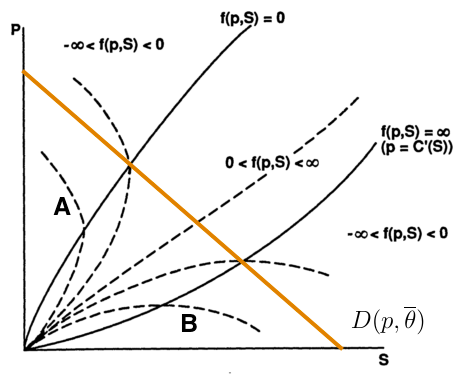
\includegraphics[width=8cm]{figintro/KMboundaries.png}
\caption{\small{This graph is adapted from the original paper by Klemperer and Meyer and illustrates the admissible region of solutions to the differential equation so as to verify the constraints on the slope of the supply function.}}
\label{KMboundaries}
\end{figure}

Therefore, the admissible set of solutions is defined by the upper bound of the demand shocks $\overline{\theta}$, in that if the solutions cross the slope boundaries before reaching the maximal shock, they cannot be accepted as solutions to the problem which constrains the solutions more strictly than the differential equation alone. In figure \ref{KMboundaries} the demand associated with the upper bound of the shocks $D(p,\overline{\theta})$ is represented in orange, and solutions A and B to the differential equation are not solutions to the problem as they reach the boundaries for smaller values of shocks.\\

The last result we will review here, is that in the case of an unbounded support of shocks, the set of equilibria is at its smallest, as it means that solutions have to have positive finite slope for every value of the shocks, and not only for a segment of the real line. \\

In some cases, for example for linear demand schedules, this set can collapse to a unique solution. \\

\section*{The case for ramping costs}

This framework models the costs as depending only on the quantity produced. In the context of electricity generation, an important type of costs that cannot be captured in such a specification of the cost function is that of ramping costs. These ramping costs refer to the fact that making production change over time induces specific costs.\\

To explain how such costs can arise, consider a thermal power plant (fossil fuels, nuclear etc.), and more precisely its core. Physically, to produce a given level of electricity, one has to maintain the core at a given temperature. To increase production, the temperature of the core has to increase. This means that when production is increased some fuel has to be lost to simply increase the temperature, this energy expenditure is not attached to any additional production.\\

This issue of ramping costs is at the heart of the choice of "quick" gas power plants to match sudden peaks in demand, where nuclear plants are more generally used for low frequency adjustments. Therefore these ramping costs are important technically on the electricity market. They are important enough for the project of European Power Exchanges named ``Price Coupling of Regions'' (PCR), which aims to develop a single price coupling solution to be used to calculate electricity prices across Europe, to consider the possibility to use load gradient orders, that is orders that condition their availability on the change in production from one hour to the next. However, at the moment of writing, PCR is still very much a work in progress \cite{EPEXPCR}.\\

Some papers have tried to estimate their values empirically, \cite{wolak2007quantifying} and more recently \cite{reguant2011welfare}. There is also a strand of litterature concerned with ramping costs, looking at the optimal price that allows to maximize the overall social welfare \cite{tanaka2006real}, that is, which price schedule allows to maximize the consumer welfare from which the production costs are substracted. This litterature does not use game-theoretical, but concerns itself with the best price signal to use in order to limit the ramping costs incurred due to varying demand, while still considering that the trajectory of demand is known. To our knowledge, there is no game-theoretical framework that has been brought to take ramping costs into account, and describe their effects on optimal strategies for the agents bidding on the market. 

\section*{Contribution}

This thesis focuses on the question of these ramping costs. In the first chapter, I tackle this question in a theoretical framework which yields predictions on the change of shape in supply functions over time as a function of the underlying uncertainty about demand shocks. The second chapter then introduces methods to study the shape of supply functions as observed on the French electricity market for data from 2011 to 2013, as well as methods to estimate the uncertainty contributed by the weather. The third chapter applies these methods to test these theoretical predictions on actual market data. The second and third chapters have been co-written with Henri de Belsunce, who finished his PhD in 2015 at the Munich-based Max Planck Institute for Innovation and Competition, under the supervision of Prof. Dr. Klaus M. Schmidt.\\

The first chapter focuses on what the introduction of ramping costs in a theoretical framework brings to the table. Our main contribution is to build and justify how these ramping costs can be tackled theoretically. First, we note that going to a continuous time descritption of the problem allows us to bring to the litterature about supply function equilibria powerful mathematical tools mostly used in option pricing, that is stochastic dynamics: we want to model ramping costs, i.e. costs associated to the variation in production, while retaining the key ingredient brought by \cite{KM}, i.e. the uncertainty, through the use of brownians, and more precisely, It\={o} processes. In so doing we face the issue that one cannot derive a brownian, and bring our second contribution, a physical argument about how power plants function that effectively operates as a low pass filter on our stochastic processes, and allow us to continue to build a tractable model of ramping costs under uncertainty. Third, we find in the litterature a specification of It\={o} processes that allows the model to remain tractable. \\

From these technical contributions we obtain our economic contributions in having a rich tractable model that yields results that contrast strongly with past results from the litterature. First, our solutions are unique, which contrasts with the usual continuum of Nash equilibria in the supply function equilibria litterature. Second, our solutions are not ex-post optimal, meaning that gathering information about the expected future evolution of demand yields different optimal strategies for suppliers, which in turn means that producers in our framework have a motive for submitting different supply functions from one time step to the next. Third, we have closed form solutions which yield specific predictions about the evolution of bids under uncertainty, namely that when uncertainty increase, suppliers submit steeper supply schedules in order to transmit more of these shocks to changes in price and not quantities, which are costly due to the existence of ramping costs. Finally, and less importantly, our framework justifies the existence of negative prices \footnote{Note that such negative prices happen, a few hours a year for example in France or Germany, for example in 2017 there were 146 such hours on 24 days in Germany \cite{epexnegP}} by producers being willing to pay consumers to consume more in order to avoid facing large variations in production, in contrast to everywhere positive schedules in the case of the supply function equilibria litterature. These results open the door to models being able to differentiate between day-ahead and intraday markets and therefore to offer a framework in which their interactions might be possible.\\

In the rest of the thesis the goal is to test our predictions on data from the French day-ahead market. In so doing, as our theoretical predictions are mainly about the effect that the amount of uncertainty has on the slope of the optimal supply schedule, we separate the issue of building proxies for this uncertainty in our second chapter, and the actual analysis of the evolution of bids on these proxies in the third chapter.\\

In the second chapter our main focus is on analyzing our data, on building a way to describe it, and on building proxies for the uncertainty that producers face about the residual demand they have to anticipate when bidding on the day-ahead market. \\

First, we note that aggregate supply functions on the day ahead market cannot be well captured by parametric functions. Therefore we devise a way to describe them non-parametrically: we note that although they cannot be captured parametrically, they still have a rough S shape, and therefore four main parts, two extremal sections, and two interior ones separated by the inflection point of the curve in its middle secion. We define the transition points between these sections as the points of maximal absolute value for the derivative and second derivative of the supply schedules. This definition relies on kernel density estimates, and is therefore non-parametric. We observe that by using 5 such points, we are able to capture about 98\% of the intrisic variability of the supply schedules, and stop there although our method can be used to define more non parametric points. This method allows us to define points that we consider comparable across auctions, that allow use to perform cross-sectional analysis of our data in the third chapter. \\

Second, we build proxies for the amount of weather uncertainty that producers face and variables that capture information that suppliers have before bidding and should therefore be controlled for. For the information available to suppliers, we note that the effect of weather on the demand, and more importantly temperature, is well understood and that we need to control for it. To do so we build an effective temperature for France, as an average of the localised temperature weighted by the population of the spatial region considered, in order to capture the overall effect temperature has on heating.\footnote{France has a high level of electric heating overall, which means that demand for electricity is quite sensitive to temperature.} The rest of our focus is on building a proxy for the uncertainty concerning renewable production. To do so we analyze spatialized wind and sunlight data, and study it's spatial structure. We argue that spatial autocorrelation is a proxy for the uncertainty associated with weather forecasts, noting that if this data displays more spatial gradients, it is likely to be of a lesser quality due to the numerical nature of the weather simulations used to predict the weather, and therefore more uncertain.\\

Our contribution in the second chapter is to provide a non parametric way to define comparable points across auctions, and a measure of the uncertainty associated with weather forecasts.\\

In the third chapter, we focus on building the main proxy for the uncertainty faced by producers, and then on analyzing how the bids evolve relative to these proxies.\\

We note that the main uncertainty is about the shape of the demand schedules itself. Therefore we consider data available to the producers and regress the demand schedules on these variables. Next, we study the residuals of these regressions, and more specifically note that they are heteroskedastic. We leverage this, regressing the square of these residuals on our variables, in order to predict the expected amplitude of the residuals, that is the amplitude of the uncertainty of the demand schedule regression.\\

We then study the effect of our different proxies for uncertainty on the slope of the supply schedules, and note that if our proxies about the weather uncertainty (through the channel of renewable production) have the expected effect, the results are less clear cut for our residuals on the demand schedules. As we are working with full blown schedules in the quantity-price plane, we perform our residual analysis both on the prices and the quantities. We therefore obtain estimates for the uncertainty pertaining to the position of a given point of our demand schedule either in price or in quantity. In our theoretical framework, we make the strong assumptions that demand schedules are linear, and that demand shocks are additive, i.e. they do not impact the slope of the demand schedules. These assumptions yield that we cannot differentiate between shocks in price or quantity, and that they should have effects in the same direction: more uncertainty implying steeper supply curves to reduce the amount of fluctuations in production. However we observe that the effects of price and quantity uncertainty as estimated by our residuals' method yield opposite effects. Both of these assumptions, although required to obtain closed form results, are clearly not satisfied by our data, and we think that this is a clear path for improvement of the model.  \\

The contribution of the third chapter is to provide a way to estimate the uncertainty about the demand schedules faced by suppliers, and to estimate how this uncertainty affects the shape of the supply schedules at different points along its overall length, i.e. we provide a framework to describe how the functional form of schedules is affected by estimates of the uncertainty faced by suppliers.\\





 
%%%%%%
%
%%%%%%
\renewcommand{\thesection}{\arabic{chapter}.\arabic{section}}
\chapter{Dynamics of the Electricity Day-Ahead Market : Supply Function Equilibria and Ramping Costs}
\label{chap:ch1}
\cleardoublepage
\pagestyle{fancy} 
\fancyhead{} 
\rhead[]{\textsl{The Design of Teacher Assignment: Theory and Evidence}} \lhead[The Design of Teacher Assignment: Theory and Evidence]{}

\fancyfoot{}
\fancyfoot[RO]{%
		\labeledflipbookframe[0][0.5]{example_frames/plus_}[pgf][0.2]{r}{\thepage}{2em}%
	}
	\fancyfoot[LE]{%
		\labeledflipbookframe[0][0.5]{example_frames/cross_}[pgf][0.2]{l}{\thepage}{2em}%
}
%\renewcommand{\tabularxcolumn}[1]{m{#1}}
%\newcolumntype{Y}{>{\centering\arraybackslash}X}
%\newcolumntype{R}{>{\flushright\arraybackslash}X}



\renewcommand{\thesection}{\arabic{chapter}.\arabic{section}}



\chapter{Dynamics of the Electricity Day-Ahead Market : Supply Function Equilibria and Ramping Costs}
\label{chap:ch1}
\cleardoublepage

\doublespacing
\section{Introduction}
\subsection{Litterature review}
The electricity markets have flourished in Europe during the 1990s during the wave of privatisation. The argument for their creation was one of competition, that was supposed to bring lower prices to the end consumer of electricity.\\

An important specificity to the economics of electricity is that electricity cannot be stored in large amounts, which in turn implies that at every moment production and consumption have to match. This means that in order to have a working electric grid, that is one that can produce electricity for high levels during the winter and lower levels in summer, one has to have production units ready to be turned on if the demand is high enough, but turned off otherwise. This in turn means that although their existence is required, it is difficult to see how to marginal cost pricing can cover their investment costs, which has been a long running argument in the litterature \cite{boiteux1960peak}. For this reason, from the very beginning the issue of the market design was deemed to be crucial to insure that the wished for outcome of the privatization wave came to fruition \cite{green1991reshaping}. \\

Most countries having open the production of electricity to competition have implemented day-ahead markets. As said above, the production and the consumption have to match constantly. The very short term matching is done by automating tiny adjustments around what a producer is already producing in order to match the fluctuating consumption. To plan which plant should be online at which hour of the day however, the day-ahead markets come in. The idea is that producers and big consumers of electricity (either for themselves, or as aggregators of the individual consumptions) are asked to bid demand or supply functions respectively. The market operator then aggregates the demand and supply curves, which yields an equilibrium giving the price and quantities to be produced for each producer.  \\

There has been an active litterature trying to model and measure the market power of oligopolists on these newly created markets \cite{Newgreen, newbery1998competition, green1999electricity}. The models have mainly been based on Klemperer and Meyer 1989's Econometrica founding paper about supply function equilibria \cite{KM} (henceforth known as KM). 

This paper builds upon previous results about competition in supply schedules without uncertainty \cite{grossman1981nash}, which yielded a very high multiplicity of equilibria. KM add a key ingredient : uncertainty about the demand schedule facing the suppliers. This addition reduces greatly the multiplicity, and adds more structure to it, although in this framework there is still a continuum of Nash equilibria, which are always pinned between Cournot and Bertrand outcomes. \\

Groundbreaking and fertile, the original model by KM studied how demand uncertainty collapses dramatically the set of available supply function equilibria to a well defined continuum when contrasted to the case of competition in supply schedules without uncertainty \cite{grossman1981nash}. These equilibria are always pinned between Cournot and Bertrand outcomes. This continuum collapses further to a single Nash equilibria by considering an infinite support of demand shocks. All of these equilibria are ex-post optimal, meaning that changes in anticipated demand shocks do not impact the actual solutions, but only the parts of the solutions that are actually explored as shocks realize. In this setup markets are always efficient, a very strong result. \\

The electricity markets litterature has embraced this framework because it is considered to capture some of the structure at play in the electricity markets : the producers do not know what demand they are going to face when they choose their supply schedule, the demand side is considered much less sophisticated than the supply side, and their demand schedules can therefore be considered to some extent as being exogenous. Some have argued that the schedules submitted in the real markets are discrete and that this discrete nature makes their modelling as continuously differentiable schedules is both incorrect and yields different results from discrete ones \cite{von1993spot}. However recent results suggest that with a sufficient amount of steps both approaches converge \cite{holmberg2008supply}, and indeed we see that recent implementations of the market rules increase the number of steps allowed for a single bid, and consider that these points are linearly joined instead of stepwise.\\

One of the mose striking aspects of the supply function equilibria approaches is, as was alluded to above, the multiplicity of Nash equilibria. This result has been generally viewed as the source of the danger of tacit collusion in electricity markets : if there is a continuum of nash equilibria, repeated interactions are feared to be conducive to a convergence of bidding strategies towards the most profitable equilbria \cite{bolle1992supply}. \\

Furthermore, these models abstract away some of the details of the actual markets, reason for which authors which try and evaluate the market power of producers on the electricity markets view their endeavour as painting the situation with an optimistic brush \cite{Newgreen}. \\

Here we will tackle the points raised in the last two paragraphs to some extent. We propose to consider a technical reality of the operating of power plants : their cost structure is history-dependant, more precisely, producing a quantity $q_1$ does not entail the same cost if the previous quantity produced was already $q_1$ or if the previous quantity was different from it. Raising or decreasing production in and of itslef imply costs. By introducing these costs we aim to produce a model capable of capturing more precisely the competition that arises in the electricity markets, and in so doing we will show that the continuum of equilibria caracteristic of supply function equilibria under uncertainty collapses to unique equilibria, which in turn allows us to comment on the question of tacit collusion.\\


%
%One traditional understanding for the role of markets is that a market allows to aggregate information that would be otherwise dispersed. When applying this view to the electricity markets, the litterature has regarded the existence of the capacity market as a way to aggregate information about investment costs when building a plant, the existence of the forward market as a way to aggregate information about the fixed costs, and the existence of the spot market as a way to aggregate information about marginal costs. \\
%
%
%At the same time, the litterature as well as the industry is well aware of the existence of ramping costs, that is costs that depend on the variation of production. We think that the two spot markets can be understood as aggregating information about marginal costs and ramping costs. In this paper we model the day-ahead market using the supply function equilibria framework and considering that there exists ramping costs. This allows us to obtain unique solutions, in contrast to the usual continuum, and to describe the dynamic evolution of the optimal bid in a symmetric oligopoly. It also opens the possibility to distinguish between day-ahead and intraday markets. \\
%
%%However, the spot market is actually divided into two markets : the day-ahead market and the intraday or balancing market, that the litterature does not differentiate clearly.
%
%The supply function equilibria litterature has been active since the seminal paper by Klemperer and Meyer in 1989 \cite{KM} (henceforth known as KM). In the wake of the electricity industry liberalisation, authors, notably Green and Newbery in 1992 \cite{Newgreen}, have used this framework to evaluate the expected level of competition and argue for certain regulatory paths. \\

\subsection{The day-ahead markets}

On the electricity day ahead markets, producers are generally required to submit supply schedules once a day for all the auctions taking place during the next day. The APX (England) and the EPEX (Austria, France, Germany and Switzerland) markets allow hourly auctions \cite{apx,epex}, and EPEX allows for bids comprising up to $256$ price quantity combinations, effectively approximating smooth supply functions. Producers can submit different supply schedules for each individual auction, but every bid must be placed at the same time one day in advance for each block of 24 hours. Customers go through the same process and submit their demand schedules, then the market operator matches supply and demand for each auction. Producers thus have to submit schedules facing uncertain demand, this is the reason for the popularity of supply function equilibria approaches to the electricity market.\\   

However, on this market, bids change from auction to auction. From the point of view of KM's model, this should happen only through a coordination of agents agreeing to collectively swap from one Nash equilibrium to another in the available continuum. Describing these dynamics, however, is increasingly important as the energetic mix is bound to include an increasing fraction of renewables. Power production can be separated in two classes: dispatchable and non-dispatchable technologies. Nuclear, coal, land-fill gas or hydroelectric power generation are mainly dispatchable as one can actually choose their level of production whereas the two rising stars of renewable energy, namely wind and solar, are non-dispatchable: they react to weather conditions. Having these technologies in the mix introduces uncertainty on the production side, which comes down to dispatchable units facing a more uncertain residual demand \cite{Boyle}. In this paper we want to explore how to model these dynamics. \\

Electricity production faces very specific technological constraints. These constraints, generally labelled as ramping costs, vary across production technologies, and have yet to be captured in a model. We propose to do so by introducing a multivariate cost function, depending as always on the quantity produced, but also on the rate at which production varies: $C(S,\frac{dS}{dt})$. We call this class of cost functions dynamic cost functions.\\

All power plants face maintenance costs. However part of these maintenance costs are induced by the dynamics of production, and can be seen as ramping costs. More precisely, whatever the production technology, fluctuations in production are costly. Indeed, they imply fluctuations in the temperature of the core of the power plant, thus dilation and contraction cycles of the different parts, which cause wear and tear. The industry is aware of these effects \cite{GE}, some B2B companies even specialize in minimizing the related long term costs. For example, Wartsila Power Plants, a supplier of power plants and tools to forecast long term costs, explains in a white paper \cite{Arima}: 
\begin{quote}
Increased variability in net load demand means that dispatchable generating units have to ramp considerably more steeply and deeper than traditionally, thus increasing wear and tear to components.
\end{quote}
We are going to model these ramping costs through a dynamic cost function, increasing in the absolute value of its second argument : any change in production is costly. This paper will focus on the implications of considering this type of ramping costs. Other types of ramping costs exist, for example startup costs, but they will not be studied in this paper. \\

These effects cannot be captured by traditionnal cost functions depending on the level of production alone. One needs to take into account the actual path leading to a given quantity produced. This implies that we need to impose structure on the dynamics of the system while retaining uncertainty, the key ingredient of KM's paper. To do so, we use stochastic dynamics. \\

This seemingly small addition to KM's framework has a lot of implications on the results obtained. The solutions are not ex-post optimal anymore, allowing to account more satisfactorily for the dynamics of optimal supply schedules, and our solutions are unique, even for bounded demand shocks. We also define a novel selection rule to choose from KM's continuum of equilibria. Finally these results open the possibility to distinguish intraday and day-ahead markets. \\ 

%In section \ref{litrev} we will present how this paper contributes to the litterature, i
In section \ref{heur} we will present a heuristic approach to get the intuition of the model. Then, in section \ref{math} we will introduce the mathematical tools needed to use stochastic dynamics in this context, in section \ref{monosolve} and section \ref{oligosolve} we will solve the monopoly and the symmetric oligopoly cases while considering that producers have information about the overall distribution of shocks during the day, but do not have information about differences in the shocks at different dates. Finally in section \ref{dynamics} we will discuss the dynamic variation of the optimal bids, while sections \ref{disc} and \ref{ccl} will respectively cover a few implications of these results and conclude the paper.  

%\section{Litterature Review}\label{litrev}
%TO BE FILLED
\section{Heuristic Description of the Model}\label{heur}
In this section the essence of the model is presented before introducing the proper mathematical tools needed to treat this problem rigorously in the next section. It is thought of as an overview of the mathematical methods that are going to be used, as a way to give a sense of the intent of the modelling choices.\\

As in KM's setup, the aim is to model an oligopoly facing uncertain demand, taken as exogenous. Before the demand shocks are realized, each firm needs to commit on a strategy. Firms also incur costs that not only depend on the level of production but also on the evolution of the production given its anterior level produced. \\

More formally, the producer, as in KM, faces uncertain demand, $D(\theta,p)$, with $\theta$ a stochastic shock to the demand and $p$ the price. We add to that both ramping costs and uncertain dynamics of demand. As we want to keep the key ingredient of KM, the introduction of uncertainty, but take into account the dynamics of this uncertainty, of these demand shocks, we need to add more structure.\\

Consider the following notation, where $\theta(t)$ denotes the value of the stochastic shock at time $t$, whereas $\Theta$ denotes the family of all available time trajectories of our demand shocks. \\

In the real market, bidders submit a finite number of bids once a day, and face the ramping costs inter-period, that is, when production has to be adjusted to reach the subsequent market outcome. The first bit of structure we introduce is that we are going to assume that time is continuous. The second is that ramping costs are incurred continuously, and can be thought of as costs depending on the variation of production over time. Finally we consider that bidders are allowed to submit a different supply schedule for every point in time between $0$ and $T$. This amounts to being asked to submit a surface of strategy in the price-quantity-time space for the next day. \\

The producer maximises her expected profits, and we consider here the simplest case in which the distribution of shocks is static, that is that the distribution of probability of shocks does not depend on time, and the producer is asked by the market operator to submit the same supply schedule for every point in time a day in advance. In an oligopoly, the program maximised by producer $i$ is therefore:

\begin{equation}
\displaystyle{\max_{S_i(p)}}~\mathbb{E}_{\Theta}\left[\int_{0}^{T} \left(p(\theta(t))S_i(p(\theta(t))) -C\left(S_i(p(\theta(t))),\frac{dS_i(p(\theta(t)))}{dt} \right)\right)dt\right]
\end{equation}
with $p(\theta(t))$ the price given the demand shock $\theta(t)$ at date $t$, $S_i(\cdot)$ the supply schedule of producer $i$ and $C(\cdot,\cdot)$ the dynamic cost function. Note that the price depends on $t$ only through $\theta(t)$, i.e. a given level of demand shock implies a given price.  \\

The goal of this section is to provide a first run through of the model, therefore we will not describe here the conditions that must be verified by the different terms of the model. We will simply assume that the dynamic cost function is additively separable between a static and a ramping term, $C(S_i,\frac{dS_i}{dt})=C_s(S_i)+C_r(\frac{dS_i}{dt})$, and that the demand shocks $\theta$ are bounded in $[\underline{\theta},\overline{\theta}]$. Lastly we require the ramping term $C_r(\cdot)=\frac{\gamma}{2}(\cdot)^k$ for clarity, and $k\geq2$ an integer. We distribute the expectation operator and write that $\frac{dS_i}{dt}=\frac{dS_i}{dp}\frac{dp}{d\theta}\frac{d\theta}{dt}=S_i'\cdot \dot{p}\cdot \frac{d\theta}{dt}$, with $X'$ the derivative of univariate function $X$ with respect to its argument, $\dot{X}=\frac{dX}{d\theta}$. \\

With this setup, by distributing the expectation operator over all possible trajectories of shocks, we are able to rewrite the problem without having time $t$ appear explicitly. This point is crucial, as it is what will let us use mathematical tools that will yield our unicity results. The maximisation program can indeed be written as follows :
\begin{equation}
\displaystyle{\max_{S_i(p)}}~\int_{\underline{\theta}}^{\overline{\theta}} f(\theta)\left(p(\theta)S_i(p(\theta(t))) -C_s(S_i(p(\theta(t))))-\frac{\gamma}{2}\left(S_i'\cdot\dot{p}\right)^k\mathbb{E}_{\Theta}\left[\left(\frac{d\theta}{dt}\right)^k\middle \vert \theta  \right]\right)d\theta
\label{maxbase}
\end{equation}
with $f(\theta)$ the distribution of shocks, and $\gamma$ the ramping cost parameter capturing the magnitude of the ramping costs. The expected value on the trajectory of shocks of any of the terms above that only depend on $\theta(t)$, that is the value of the shock at a point in time, can be rewritten simply as an integral over the possible values of the shock. \\

We are left with $\mathbb{E}_{\Theta}\left[\left(\frac{d\theta}{dt}\right)^k\middle \vert \theta  \right]$ as the only term that depends on the trajectory of shocks. Take for granted that this term can only depend on $\theta$ for now, this result will be defended properly in the next section. \\

Note now that producer $i$ faces a residual demand so that $S_i(p(\theta(t)))=D(\theta,p(\theta(t)))-S_{-i}(p(\theta(t)))$ which depends only on $\theta$ and $p$, $t$ does not intervene directly, with $S_{-i}$ the aggregate supply schedule of all the other producers, taken as given by producer $i$. This implies that the integrand in eq. \ref{maxbase} depends only on three variables: $\theta$, $p$ and $\dot{p}$.  The maximisation pogram is therefore equivalent to an Euler-Lagrange problem, a very well described mathematical object: $\max_p\int\mathcal{L}(\theta,p,\dot{p})d\theta$. \\

The information obtained from taking the first-order condition of an Euler-Lagrange problem yields a second order differential equation as well as two boundary conditions: $\frac{\partial\mathcal{L}}{\partial p}=\frac{d}{d\theta}\frac{\partial\mathcal{L}}{\partial \dot{p}}$ and $\frac{\partial\mathcal{L}}{\partial\dot{p}}\big|_{\underline{\theta}}=\frac{\partial\mathcal{L}}{\partial\dot{p}}\big|_{\overline{\theta}}=0$. This is why we obtain unique solutions: if the boundary conditions are not verified there exists profitable deviations. \\

In less mathematical terms, taking ramping costs into account as specified above means that for a given level of shock, the producer not only cares about the optimal level of production for this shock, but also about the optimal slope of the supply schedule at this level of production. Effectively, this means that optimal levels of production cannot be chosen independently for different level of shocks as is the case in KM, thus shrinking the continuum of equilibria. The boundary conditions' argument explains why the continuum not only shrinks, but collapses to a unique equilibrium. \\

Note that if the ramping cost parameter $\gamma$ is taken equal to $0$ we are back to KM's model: one doesn't care about the slope of the supply schedule anymore, and the problem comes down to a pointwise maximisation which therefore yields ex-post optimal equilibria. We want to stress that this means that it is not sufficient to specify the dynamics of the shocks to obtain a supply function model that would react to these dynamics, one needs to take into account ramping costs.\\

The maximisation program~\ref{maxbase} is a heuristic description of the situation. We want to model the stochastic nature of demand and of its dynamics. We do this by using It\={o} processes, a class of stochastic processes built through brownians, to describe the stochastic trajectory of the demand shocks with respect to time. The difficulty is that brownians are everywhere continuous but nowhere differentiable, therefore the way program~\ref{maxbase} is written, with a term in $\frac{d\theta}{dt}$, is a shortcut.\\

In the next section we introduce the stochastic dynamics properly without using the concept of derivative. 


\section{Stochastic Dynamics}\label{math}

As described in the previous section, we consider that bidders submit surfaces, that is supply schedules for every point in time. The reason to describe a discrete dynamic market as a continuous one is that although discrete time is conceptually more easily understood, continuous time allows to use much more powerful mathematical tools and to obtain closed form solutions, which we think are crucial in gaining intuitive insights about these dynamics. Therefore we consider that demand fluctuates continuously and that ramping costs are incurred instantaneously. This approximation would need to be tested, although it should be noted that day ahead markets operate with hourly or half-hourly periods and producers are therefore facing a reasonable amount of periods each day. \\ 

We want our shock variable to evolve over time in a random fashion. The class of mathematical objects used to describe this are stochastic processes. The simplest stochastic process one can think of, and indeed the most important historically, is a Brownian motion process. \\

Unfortunately, Brownian processes are unbounded, and cannot therefore be used to describe the dynamics of the electricity market in which demand shocks, denoted $\theta(t)$, are bounded: there are no days for which demand is null nor are there days for which demand tends towards infinity. The structure to be imposed on the dynamics of the shocks has to imply bounded shocks.\\

%Our strategy to describe a discrete process as a continuous one is as follows. We know which class of stochastic process we want to use in continuous time that is rich enough to yield interesting dynamics yet still manageable mathematically speaking. We are therefore going to take the discrete approximation of this continuous process, discuss this discrete description, and then decrease its timescale towards $0$ to converge towards the stochastic process. We are first going to describe the target stochastic process that we will be using throughout this paper, before illustrating how we go from a discrete description to a continuous one. \\
%
%In the electricity market, demand shocks, denoted $\theta(t)$, are bounded: there are no days for which demand is null nor are there days for which demand tends towards infinity. The structure to be imposed on the dynamics of the shocks has to imply bounded shocks. \\

\subsection{The stochastic process}
A richer set of stochastic processes is the set of It\={o} processes.\\

A simple It\={o} process one can consider that leads to bounded shocks is defined by the following stochastic differential equation (SDE):
\begin{equation}
d\theta(t)=-2\theta(t) dt+\sqrt{1-\theta(t)^2}dB_t
\label{eqSDE}
\end{equation}
with $B_t$ a brownian and $dX$ an infinitesimal variation of quantity $X$. \\

Observe that this SDE is formed by a deterministic mean-returning term $-2\theta(t) dt$ and a bounded stochastic one $\sqrt{1-\theta(t)^2}dB_t$. As $\theta(t)$ approaches $-1$ or $1$ the stochastic term goes to $0$, thus $\theta(t)\in [-1,1]$.  Without loss of generality we can restrain ourselves to this special case. Other bounded supports, $\theta\in[\underline{\theta},\overline{\theta}]$, can be captured through renormalisations of $\theta$. \\

Such a stochastic process has a distribution of probability $f(\theta)$ given by Fokker-Planck's equation, easily solved here. In the general case of an It\={o} process given by SDE \ref{sdegen}, one obtains in \ref{FokP} the generic Fokker-Planck equation for its distribution of probability $f(\theta,t)$:
\begin{flalign}
&d\theta=\mu(\theta,t)dt+\sigma(\theta,t)dB_t&\label{sdegen}\\ 
&\frac{\partial}{\partial t}f(\theta,t)=\frac{\partial}{\partial \theta}(\mu(\theta,t)f(\theta,t))+\frac{1}{2}\frac{\partial^2}{\partial \theta^2}(\sigma(\theta,t)^2f(\theta,t))&\label{FokP}
\end{flalign}

Here, for SDE \ref{eqSDE}, this yields that $f(\theta)=\frac{3}{4}(1-\theta^2)$ on $[-1,1]$ and $0$ elsewhere.\\

\subsection{The ramping costs}
\label{sec_ramping_costs}
In the rest of the paper we are going to consider quadratic ramping costs. More precisely we consider the costs induced by fluctuations in the production level. As described in the introduction, fluctuations imply increased wear and tear, whether the production is increasing or decreasing. In addition, these ramping costs are null in the absence of fluctuations. This means that they can be captured by a function $C_r(\cdot)$ verifying $C_r(0)=0$, $C_r(\cdot)\geq0$ and increasing in the absolute value of its argument. In the abscence of more detailed knowledge about the actual shape of these ramping costs, it seems reasonable to consider a quadratic cost function, that is the first term in a Taylor expansion of the actual real ramping cost function. \\

We cannot compute $\frac{d\theta}{dt}$ as it appears in Eq.~\ref{maxbase}, as a stochastic process, although everywhere continuous, is nowhere differentiable. The goal of this section is to express properly the maximisation program of the producer that we presented rapidly in Eq.~\ref{maxbase}, and most importantly, to introduce properly how we can work in continuous time with a cost function which depends on fluctuations, and fluctuations which are nowhere differentiable.\\

We are therefore going to first consider the discrete case of a random walk of timestep $\Delta t$ which converges towards the It\={o} process \ref{sdegen}, using the Euler-Maruyama approximation, a generalisation of the Euler method to stochastic differential equations. We consider a Markov chain $Y$ defined as follows : 

\begin{equation}
\Delta Y_n=Y_{n+1}-Y_n= \mu(Y_n,n \Delta t)\Delta t+\sigma (Y_n,n \Delta t)\Delta B_n
\end{equation}
where $\Delta B_n=B_{(n+1)\Delta t}-B_{n\Delta t}$. These $\Delta B_n$ are \emph{i.i.d.} normal random variables of mean $0$ and variance $\Delta t$. Note that as $\Delta t$ is taken towards $0$, this Markov chain converges towards its underlying stochastic process defined by eq.(\ref{sdegen}).\\

The ramping costs are taken as quadratic in the variation of the production, and also depend on a ramping cost parameter $\Gamma(\Delta t)$, that is the cost per unit of quadratic variation at horizon $\Delta t$, so we compute the following quantity : 

\begin{equation}
\mathbb{E}\left[\frac{\Gamma(\Delta t)}{2}\cdot\left(\frac{Y_{n+1}-Y_n}{\Delta t}\right)^2\middle \vert Y_n  \right]=\frac{\Gamma(\Delta t)}{2}\cdot\frac{\sigma (Y_n,n \Delta t)^2}{\Delta t}
\label{markovariation}
\end{equation}

For this quantity to converge to a finite value when the Markov chain is taken towards its underlying stochastic process we have to consider that for small enough timescales, the ramping cost parameter $\Gamma(\Delta t)$ is linear in $\Delta t$, i.e. $\Gamma(\Delta t)=\gamma \Delta t +o(\Delta t)$. Mathematically, if $\Gamma(\Delta t)$ had a slower than linear relationship at small timescales, the ramping costs would diverge, and if it was faster they would converge to $0$. A physical constraint, namely thermal inertia, ensures that the ramping cost parameter does actually behave in this way\footnote{Ramping costs come from thermal fluctuations in the core of the plant. Therefore we have to describe how temperature responds to fluctuations in production. Thermal inertia acts as a low pass filter, meaning that it smoothes out fluctuations on short timescales. Think about heating a saucepan full of water: although lighting the stove is almost instantaneous, the temperature of the water being heated increases only progressively, in an exponential fashion that is therefore linear in time for short timescales. }. \\

%For more details about this, see appendix \ref{rampingcostsappendix}.\\

Consider for now that the mean function $\mu$ and the variance function $\sigma$ from eq. \ref{sdegen} do not depend on time explicitly and are therefore written $\mu(\theta)$ and $\sigma(\theta)$. Consider now a transformation $T(\cdot)$ that we apply to the Markov chain $Y$. Then:
\begin{equation}
\mathbb{E}\left[\frac{\Gamma(\Delta t)}{2}\cdot\left(\frac{T(Y_{n+1})-T(Y_n)}{\Delta t}\right)^2\middle \vert Y_n  \right]= \mathbb{E}\left[\frac{\Gamma(\Delta t)}{2}\cdot\left(\frac{T(Y_{n+1})-T(Y_n)}{Y_{n+1}-Y_n}\cdot\frac{Y_{n+1}-Y_n}{\Delta t}\right)^2\middle \vert Y_n  \right]    
\label{markovcomposed}
\end{equation}

And in the limit where the markov process $Y$ converges towards the It\={o} process $\theta$ of equation \ref{sdegen}:
\begin{equation}
\lim_{\Delta t \to 0}\mathbb{E}\left[\frac{\Gamma(\Delta t)}{2}\cdot\left(\frac{T(Y_{n+1})-T(Y_n)}{\Delta t}\right)^2\middle \vert Y_n  \right]= \frac{\gamma}{2}\cdot T'(\theta(t))^2 \cdot \sigma(\theta) ^2   
\label{limitmarkovcomposed}
\end{equation}

We apply this result to the problem at hand, that is that we evaluate the ramping costs in the case where the demand shocks are given by eq. \ref{eqSDE}: 
\begin{equation}
\lim_{\Delta t \to 0}\mathbb{E}\left[\frac{\Gamma(\Delta t)}{2}\cdot\left(\frac{\Delta S_i(p(\theta(t)))}{\Delta t}\right)^2\middle \vert \theta(t)  \right] = \frac{\gamma}{2}\cdot S_i'(p(\theta(t)))^2\dot{p}(\theta(t))^2 (1-\theta^2)
\label{markovtosde}
\end{equation}
with $X'$ the derivative of quantity X with respect to its argument and $\dot{X}$ its derivative with respect to $\theta$. Note that we considered here that the variance term $\sigma(\theta)=1-\theta^2$ depends only on $\theta$ and not explicitly on $t$, which in turn implies that the strategy $S_i$ does not depend explicitly on $t$ either. \\

Let us consider the case where the strategy and the variance depend explicitly on time, and are thus written $S_i(p(\theta(t),t),t)$ and $\sigma(\theta,t)$ respectively.  By using a first order expansion as before, the ramping cost function can be approximated as follows:
\begin{small}
\begin{eqnarray}
\lim_{\Delta t \to 0}\mathbb{E}\left[\frac{\Gamma(\Delta t)}{2}\left(\frac{\Delta S_i(p(\theta(t),t),t)}{\Delta t}\right)^2\middle \vert \theta(t)  \right] &=& \lim_{\Delta t \to 0}\mathbb{E}\left[\frac{\gamma}{2} (\partial_1S(p(\theta(t),t),t)\partial_1p(\theta(t),t))^2\frac{\Delta\theta^2}{\Delta t}+\mathcal{O}(\Delta t)\right]\nonumber\\
&=& \frac{\gamma}{2} (\partial_1S(p(\theta(t),t),t)\partial_1p(\theta(t),t))^2 \sigma(\theta,t)^2
\label{markovtimedep}
\end{eqnarray}
\end{small}
with $\partial_iX$ the partial derivative of quantity $X$ with respect to its $i^{th}$ argument. See Annex. \ref{stochasticdyn_proof} for a more details on this derivation.\\

Now, we can write down the instantaneous expected value of the profit of producer $i$ if the demand shock is $\theta(t)$, $\pi^e_i(t, \theta(t))$, that is the profit that one expects to obtain when demand is at $\theta(t)$ given the expected value of the ramping costs:
\begin{small}
\begin{equation}
\pi^e_i(t,\theta(t))= p(\theta(t),t)S_i(p(\theta(t),t),t) - C_s(S_i(p(\theta(t),t),t)) -\frac{\gamma}{2} \partial_1S_i(p(\theta(t),t),t)^2\partial_1p(\theta(t),t)^2 \sigma(\theta,t)^2
\label{instantprofit}
\end{equation}
\end{small}

Lastly we have to write down the expected profit for a day's worth of submitted strategies. Let us consider that the chosen unit of time is the day. Therefore, the total expected profit $\Pi^e_i$ writes: 

\begin{eqnarray}
\Pi^e_i&=&\int_0^1\mathbb{E}_{\theta(t)}[\pi^e_i(t,\theta(t))]dt\nonumber\\
&=&\int_0^1\int_{\underline{\theta}}^{\overline{\theta}}f(\theta,t)\Big[p(\theta,t)S_i(p(\theta,t),t) - C_s(S_i(p(\theta),t)) \Big.\nonumber\\
&&\left.-\frac{\gamma}{2} \partial_1S_i(p(\theta,t),t)^2\partial_1p(\theta,t)^2 \sigma(\theta,t)^2\right]d\theta dt
\label{totprofit}
\end{eqnarray}

\subsection{Discussion of the approximations}
We want a tractable mathematical formulation of the dynamic problem faced by producers on the electricity market. To achieve this we seek to describe the discrete real life problem by an approximated continuous one. We first use two technological facts: fluctuations in production are costly and these costs decrease linearly in time for short timescales. We then rely heavily on first order expansions of the different terms we have to compute.  

\subsection{The maximisation program}
Here, we consider that the dynamics of demand shocks are given by eq.(\ref{eqSDE}), and that therefore  $\sigma(\theta,t)^2=\sigma(\theta)^2=(1-\theta^2)$.\\

We now introduce the different conditions that have to be satisfied by the various terms in this problem. First, on most electricity markets, schedules must be increasing, therefore here we take $S_i'(\cdot)\geq0$. Second, the aggregate demand is non negative as consumers do not have production facilities at their disposal: $D(\theta(t),p(\theta(t)))=\sum_iS_i(p(\theta(t)))\geq0$. Last, we consider that the shocks $\theta$ are ordered so that the demand is increasing in $\theta$, i.e. $\frac{\partial D}{\partial\theta}\geq0$, and that the price has to weakly increase with the shocks, i.e. $\dot{p}\geq0$. Our initial stochastic maximisation program can thus be rewritten as a regular optimal control problem: 

\begin{equation}
\displaystyle{\max_{S_i(p)}}~\int_{-1}^{1} f(\theta)\left(p(\theta)S_i(p(\theta)) -C_s(S_i(p(\theta)))-\frac{\gamma}{2}(1-\theta^2)\left(S_i'(p(\theta))\dot{p}(\theta)\right)^2\right)d\theta
\end{equation}
\begin{eqnarray} 
s.t.\hspace{2cm}&S_i'(\cdot)\geq0 \nonumber\\
&\dot{p}\geq0\\
&D(\cdot,\cdot)\geq0 \nonumber\\
\end{eqnarray}

The next section solves this problem for a monopoly. 



\section{The Monopoly}\label{monosolve}
Let us consider that the aggregate demand is linear, that is: $$D(\theta(t),p(\theta(t)))=a\theta(t)+b-p(\theta(t))$$
with $a$ and $b$ parameters taken to describe any bounded support of shocks given the stochastic dynamics introduced in the previous section for which $\theta\in[-1,1]$. Here $(a\theta+b)\in[b-a,b+a]$.\\

In a monopoly situation we have $S=D(\theta(t),p(\theta(t)))$, therefore the constraints reduce to: $$\dot{p}(\theta)\in[0,a],~\textrm{and }p(\theta)\leq a\theta+b$$
where $\dot{X}$ corresponds to $\frac{dX}{d\theta}$. \\

Consider in addition that the static cost function is also quadratic: $C_s(S_i)=\frac{\lambda}{2}S_i^2$. The maximisation program is rewritten as: 
\begin{equation}
\displaystyle{\max_{p(\cdot)}}~\int_{-1}^{1} f(\theta)\left(p(\theta)(a\theta+b-p(\theta)) -\frac{\lambda}{2}(a\theta+b-p(\theta))^2-\frac{\gamma}{2}(1-\theta^2)\left(a-\dot{p}(\theta)\right)^2\right)d\theta
\end{equation}
\begin{eqnarray}
s.t.\hspace{2cm}&\dot{p}(\theta)\in[0,a] \nonumber\\
&p(\theta)\leq a\theta+b \nonumber
\end{eqnarray}


\subsection{Results}
\begin{proposition}\label{monopequilibria}
The solution exists, is unique, and has the following form:
\begin{equation}
\forall \theta \in [-1,1]~p^*(\theta)=a\frac{4\gamma+1+\lambda}{4\gamma+2+\lambda}\theta+ b\frac{1+\lambda}{2+\lambda} \label{monopsol}
\end{equation}
The optimal schedule is parametrised by $\theta$ so that $S(p(\theta))$ is formed by the points of coordinate $(a\theta+b-p(\theta),p(\theta))$. Its equation is given by:
\begin{equation}
S^*(p)=\frac{1}{4\gamma+1+\lambda}\left(p+\frac{4\gamma}{2+\lambda}b\right) \label{monopS}
\end{equation}
\end{proposition}

\begin{proof}
See annex \ref{annexmonop}. \qed
\end{proof} 

We present in Fig.~\ref{monopsup} the results obtained for increasing values of the ramping cost parameter $\gamma$, starting at $\gamma=0$ in black and moving progressively from black to blue to red to green. \\

As expected, adding these inertial costs narrows down the domain of attainable quantities produced, as a larger quantity domain implies larger incurred ramping costs.\\

More interesting is the way the quantity domain is narrowed down. The domain of prices increases conversely, so that the solutions are steeper than the traditional monopoly situation, bringing the schedules ever closer to a Cournot-like situation. In addition, the optimal supply schedules do not depend on $a$, the parameter determining the width of the possible shocks, but only on $b$ which defines the average value of the shocks. \\

One can then study the comparative statics when the values for $a$ and $b$ are varied, as illustrated in Fig. \ref{monopab}. In particular, if we consider an increase in $a$ without changing $b$, the solution is represented by the same ``master'' function, but the explored region expands. On the other hand, if we consider a fixed $a$ but an increasing $b$, the explored length is kept constant, but the optimal schedule is translated towards the north-east region of the plane as expected intuitively: more demand implies a given mix between higher quantities and prices, which is given by the direction of the vector of translation. Note that the independence of the solution on variations of $a$ comes from the fact that we are considering comparative statics, which is very different from dynamically evolving values of $a$ and $b$, case which will be treated in detail in section \ref{dynamics}.  \\

Lastly, note that all schedules cross at a single point. These quadratic ramping costs imply a symmetric deformation of the solution without ramping costs. The limit of extremely high ramping costs is a Cournot-like schedule, i.e. a vertical one, taken at this crossing point. 

\begin{figure}[h]
\centering
\mbox{\subfigure[\small{$S^{-1~*}(p)$}] {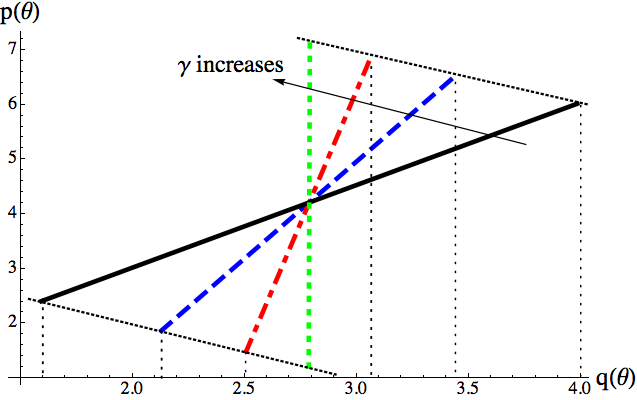
\includegraphics[width=10.cm]{figch1/monopoly_complet.png}\label{monopsup}}\quad
\subfigure[\small{$S^{-1~*}(p)$}]{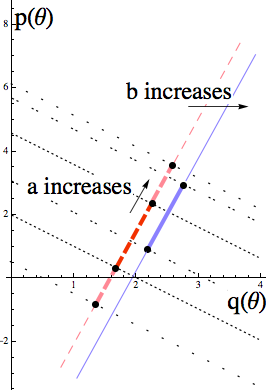
\includegraphics[width=4.5cm]{figch1/monopoly_completab.png} \label{monopab}}}
\captionsetup{singlelinecheck=off}
\caption[a b]{\small{ \textbf{\subref{monopsup}} Four optimal supply schedules are plotted. In black (full line) $\gamma=0$. As $\gamma$ increases we transition from the black curve to the blue curve (large dashes), then the red curve (mixed dashes) and then finally for $\gamma\to\infty$ to the green one (small dashes). The range of production is highlighted for each curve through the thin vertical dotted lines. 
\vspace{0.1cm}

\textbf{\subref{monopab}} The thin black dotted lines represent the extremal demand functions given $a$ and $b$, i.e. $D(\underline{\theta},p)$ and $D(\overline{\theta},p)$. From \ldots to \ldots $b$ is kept fixed while $a$ is increased, and from \ldots to \ldots $a$ is kept constant while $b$ is increased. In red (dashed) the solution for a given value of $b$. As $a$ increases, the solution widens from the thick deep red region to the thick light red one. In the case for which $a$ is kept constant and $b$ is increased the solution shifts from the dashed deep red region to the full thick blue one.   
}} 
\label{fig:monop}
\end{figure}

\section{The Symmetric Oligopoly}\label{oligosolve}

We keep the same linear demand specification as in the monopoly, therefore, with $n$ competitors one has to consider the residual demand faced by each producer: 
\begin{flalign}
&S(p(\theta))=a\theta+b-(n-1)S(p(\theta))-p&\label{condsymi}\\
&S(p(\theta))=\frac{a\theta+b-p}{n} &\label{supequ}\\
&S'(p(\theta))=\frac{a-\dot{p}}{n\dot{p}}&\\
&S''(p(\theta))=-\frac{a\ddot{p}}{n\dot{p}^3}&\label{condsymf}
\end{flalign} 
For concision, we drop the explicit dependencies of the different functions on their arguments in the following equations; $f(\theta)$, $p(\theta)$ and $S(p(\theta))$ will be noted $f$, $p$ and $S$ respectively. The maximisation program now writes:
\begin{equation}
%\begin{split}
\displaystyle{\max_{p(\cdot)}}~\int_{-1}^{1} f\bigg(p(a\theta+b-p-(n-1)S) -\frac{\lambda}{2}(a\theta+b-p-(n-1)S)^2%\\
-\frac{\gamma}{2}(1-\theta^2) \left(a-\dot{p}(1+(n-1)S')\right)^2\bigg)d\theta
%\end{split}
\label{maxoligopo}
\end{equation}
\begin{eqnarray}
s.t.\hspace{2cm}&\dot{p}\in[0,a] \nonumber\\
&p\leq a\theta+b \nonumber
\end{eqnarray}
with, as before, $\dot{X}=\frac{dX}{d\theta}$ and $X'$ is the derivative of function $X$ with respect to its argument. 

\subsection*{Results}
\begin{proposition}\label{propoligo1}
The solution exists, is unique, and has the following form:
\begin{equation}
\forall \theta \in [-1,1],~p^*(\theta) =aK_1\theta+bK_2 \label{oligosol}
\end{equation}
with 
\begin{flalign}
&\displaystyle{K_1=\frac{n\sqrt{(4\gamma+\lambda+n)^2-4n+4}-(4\gamma+\lambda+n)(n-2)}{2(4\gamma+\lambda+2n)}}& \\
&\displaystyle{K_2=\frac{\lambda(n-1)+K_1(\lambda+n)}{(\lambda+n)(n-1)+K_1(\lambda+2n)}}&
\end{flalign}
and the supply schedule has the following expression:
\begin{flalign}
&S^*(p)=\frac{1}{n}\left( p\left( \frac{1}{K_1}-1\right)+b\left( 1-\frac{K_2}{K_1}\right) \right)&
\end{flalign}
\end{proposition}
\begin{proof}
 See Annex \ref{annex1}. \qed
\end{proof}

\begin{proposition}\label{oligoslope_prop}
The slope of the supply schedule is increasing with $\gamma$ and the schedule is shifted to the right of the plane $(q,p)$ as $\gamma$ increases. This is to say that the schedule rotates around a point in the positive quadrant of the plane. 
\end{proposition}
\begin{proof}
See Annex \ref{oligopslope_proof}. \qed
\end{proof}

We are now going to focus on the graphical representation of these solutions. As in the monopoly case we obtain unique solutions of increasing steepness in the ramping cost parameter $\gamma$. When the ramping costs increase, it becomes more and more costly to allow for a large domain of potential quantities to be produced. \\

The black curve in Fig.~\ref{fig:oligop} corresponds to the limit solution when $\gamma\to0$, for which the problem gets closer to that of KM, i.e. no ramping costs. Note that as long as $\gamma\neq0$ the solutions are unique. This contrasts with the case of $\gamma=0$ which is the model presented in KM, for which there is a continuum of solutions. There is no smooth transition between our sets of solution : when considering ramping costs, there is a single Nash equilibria, even in the limit of small such costs.\\

Secondly, in their paper, Klemperer and Meyer show that in the limit of a diverging upper bound for their shocks, their continuum of solutions converges towards a unique solution. Our unique solution in the limit of small ramping costs is the same as that ok KM in the limit of infinite support of demand shocks.\\

\begin{proposition}
When $\gamma\to0$, the solution remains unique and converges towards the linear schedule available in KM's set of solutions, that is the same schedule selected with KM's selection rule obtained when considering an infinite support for the shocks.
\end{proposition}
\begin{proof}
It is straightforward to check that $K_1$ and $K_2$ have the same values as KM for $\gamma\to0$. \\
More intuitively the argument is as follows. When $\gamma\to 0$, with $\gamma>0$, we retain a unique solution although the problem itself converges towards that of KM. We should select an equilibrium present in KM's continuum. When KM take the limiting case of an infinite support of shocks they select a unique equilibrium. In our case we can do the same thing by taking $a\to\infty$. In the limit, our solution being in their set which converges to a unique equilibrium, those two selected equilibria should be equal. Now note that our solution does not depend explicitly on $a$ so that when the support is finite, we still select the same equilibria out of what is now a continuum of equilibria in KM's framework.             \qed
\end{proof}


\begin{figure}[h] 
\centering
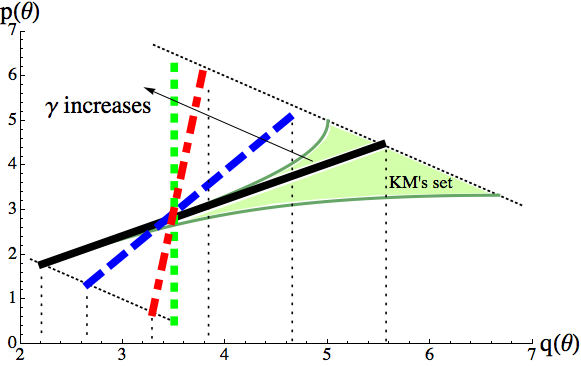
\includegraphics[width=12cm]{figch1/oligovraiKMd.png}
\caption{\small{This graph plots $S^*(p)$ for different values of the ramping cost parameter, and compares them to the set of equilibria obtained in KM's framework. Four optimal supply schedules are plotted. The black curve (full line) corresponds to the case where $\gamma\to0$. As before, as $\gamma$ increases the optimal schedules get steeper and steeper until in the limit of $\gamma\to\infty$, the optimal schedule attains a vertical slope. In addition, we show the set of available equilibria in KM's model in light green, and the extremal demand schedules in dashed black.  }} \label{fig:oligop}
\end{figure}

Intuitively, as we take $\gamma$ to $0$ we come closer to the situation captured in KM, but as long as $\gamma>0$, the producer still faces ramping costs, and therefore converges towards the only linear schedule available in KM's set, as shown in Fig.~\ref{fig:oligop}, in which we plot our solutions on top of KM's solution set in order to clarify the comparison. \\

Note that it isn't possible to transition smoothly from our model to that of KM, although they are obviously closely related. Indeed, $\forall \gamma>0$, our model yields unique solutions, but for $\gamma=0$ we return to KM's model for which there is a continuum of equilibria. There is an intrinsic discontinuity between these two models, namely, the correspondence $\Gamma(\gamma)$ associating the set of equilibria to the symmetric oligopoly problem obtained for a given value of the ramping cost parameter $\gamma$ is not lower hemicontinuous at $\gamma=0$. \\

In addition to proposing a way to take into account dynamic technological constraints, our model provides a selection rule to choose from the continuum of equilibria described in KM's seminal work, i.e. the solutions' stability to ramping costs.\\

We have here a model which solutions depend on the distribution of shocks, therefore we are able to capture the interday variation of bids by assuming that the distribution of shocks varies from day to day. In this case, there exists only one symmetric equilibria each day, function of the distribution of shocks.\\

\subsection{Discussion}

This result sheds some light on one of the questions that the electricity market literature focuses on. \\

Accounting for ramping costs induces a collapse of the equilibria set from a continuum to a unique element. \\

Most of the tacit collusion concern that is present in the literature is based on the existence of a continuum of solutions. This continuum is thought as being conducive of tacit collusion because the electricity market entails repeated interactions between producers. In this case, producers can be feared to be able to learn to pick the most profitable Nash equilibria. \\

Our result implies this pathway for tacit collusion is not available anymore. With only one Nash equilibria at any given time no learning can bring about tacit collusion. \\

We are also able to account for negative prices which was impossible in the previous framework. Such negative prices are actually observed, although rarely, on the market: producers prefer to subsidize consumption instead of decreasing production by a lot. In our framework, if the ramping costs are large enough, and the demand shocks can reach a small enough value, our solutions can yield negative values : the equilibrium price might even be below the marginal cost of production, understood here as $\partial_q C$ which by definition does not capture our ramping costs.

%
%In addition to this consideration, one must note that our unique solution rotates towards a steeper and steeper supply schedule as the ramping costs increase. However this rotation does not occur around the mean demand shock, but around a lower shock value. This means that, in expected terms, our solutions are more costly than the one selected by KMs infinite support argument. As long as the ramping costs are not too high, our solution lies in the region of the price quantity plane delimited by the continuum of solutions of KM. Therefore, for empirical work trying to estimate

In the next section we are going to present how to capture richer dynamics, and especially how the surface of bids should evolve with time when the producers have information about the anticipated variation of shocks during the day. 

\section{Dynamic behavior of the bids} \label{dynamics}
The classical supply function equilibria models, as described before, yield a continuum of Nash equilibria, and each one of those equilibria is ex-post optimal. This a very strong result that we are going to take some time to describe and comment.\\

Consider for a moment that firms competing in supply schedules reach one of the many possible Nash equilibria under such a setup, and that they commit to their schedules. Now consider that the firms face a succession of demand shocks, and that this yields a succession of market outcomes. As the Nash equilbria are ex-post optimal, it means that given the strategies played by the other firms, no firm has any regrets concerning its strategy. Knowing about the realized demand shocks does not imply any willingness to change strategy as long as other firms keep their strategies fixed, and as long as the support of shocks is not reduced ot a point (one could think of observed realisations of shocks as helping to narrow down the expected range of shocks without implying a pinpoint accuracy).\\

A corollary to this observation is that the distribution of anticipated shocks does not play any role in KM's paper, apart from its bounds. Knowing that the demand shocks are going to be drawn from distributions of high or low values does not affect the willingness to play a given strategy, as long as the support does not evolve. The little role that is played by information about shocks in KM's paper is even more counter-intuitive : to a certain extent, information about demand shocks gives rise to a larger continuum of solutions. Indeed, if one compares the equilibria available to firms for a given support $\{\theta\}_1=[\underline{\theta}_1, \overline{\theta}_1]$, noted ${S^*}_1$, to those obtained for a support strictly included in the first one $\{\theta\}_2=[\underline{\theta}_2, \overline{\theta}_2]\subset\{\theta\}_1$, noted ${S^*}_2$, then the set of equilibria will be larger in the second case, in the sense that $ {S^*}_1\restriction_{\{\theta\}_2}\subset {S^*}_2$ (where $\restriction_{\{\theta\}_2}$ denotes that the supply functions are restricted to values over $\{\theta\}_2$). \\

However, actual firms bidding on the electricity markets are known to be actively engaged in forecasting the future demand levels in order to build their strategies. Bids that we can observe on the electricity markets change from hour to hour even when demand does not vary enough to warrant a change of online plants, a consideration that could explain some of the supply schedules variations. \\

The general interpretation of KM's paper when applied to electricity markets is that for some unknown underlying process, strategies converge towards different equilibria of the set of available equilibria from hour to hour. One can note that the general intuition for strategies converging towards Nash equilibria in the first place is through either a high degree of sophistication on the part of firms, or through a more organic learning process. Neither of these two explanations can account for frequent switching from one Nash equilibria to another, out of a myriad of available options, wihtout considering some communication among firms. Furthermore, if such communication existed, it should be expected to yield the most profitable equilibria out of the available lot.\\ 

We think that this strand of argument trying to explain bids' dynamics in the light of the supply function equilibria framework is unsatisfying and we argue that forecasting demand becomes important for firms when one considers dynamic effects, that is effects that are history dependent, of which ramping costs which we model in this paper are an instance (one can think of start-up and shut-down costs as another instance of such dynamic effects). \\

The model described in the previous section doesn't account for these hourly dynamics. Here we present a way to capture these intraday variations, by considering bids that depend continuously on the time $t$. We will show that our results imply that firms are not oblivious to information about the distribution of shocks anymore, and more than that, that their strategies directly evolve with the evolution of their knowledge about uncertain furture shocks.\\


\subsection{The setup}\label{setupdyn}
Previously, the SDE (stochastic differential equation) defining the dynamics of the problem was written as: 
$$d\theta(t)=-2\theta(t) dt+\sqrt{1-\theta(t)^2}dB_t$$ 
This specification implied a stochastic trajectory for the shocks, bounded by a constant envelope. That is to mean that, lacking any knowledge of the value of the shock at a point in time close to the period under consideration, the distribution of shocks does not depend on time.\\

To account for these intraday variations we are going to define a richer SDE. \\

SDEs have been well studied and as a consequence there exists a number of families of SDEs satisfying numerous characteristics \cite{enveloppe}. The goal here is to find one SDE that will allow us to capture some of the dynamics of shocks and how this might influence strategies, while keeping it as simple as possible. Just as in the previous section, the first caracteristic that we want is to consider SDEs that imply a bounded support of shocks. This restricts our possible choice to four families out of the classical ones: Generalised Beta I, Beta, Power, Uniform. We also consider that a desirable property is that the distribution reaches 0 continuously at the bounds of its support. This restricts us further to only two families : Generalised Beta I and Beta. For tractability reasons we will focus here on the Beta family of SDEs, and more precisely on one of the simplest Beta SDE. However, we want to note that this choice stems from our focus towards solving analytically the problem at hand and obtain closed form solutions. If one were to try and estimate the distribution of shocks anticipated by firms from market data one might want to try and find which of the Beta or Generalised Beta I SDEs might match the distribution of errors between the published day -1 estimates for demand and the observed quantities.\\

Define the evolving envelope of shocks by two functions, $(\underline{\theta}(t),\overline{\theta}(t))$, respectively the lower and upper bounds of the shocks. These two functions, although very easy to comprehend, are not the most useful way to define the boundary. Instead we are going to use the average value of the shocks, and the half width of the envelope, $(\hat{\theta}(t), \omega(t))$. This means that $\underline{\theta}(t)=\hat{\theta}(t)-\omega(t)$ and $\overline{\theta}(t)=\hat{\theta}(t)+\omega(t)$. The only restriction we impose on the envelope is that we require it to be continuously differentiable, that is $(\hat{\theta},\omega)\in\mathcal{C}^1(\mathbb{R})$.\\

Consider the following SDE which is the simplest Beta SDE that we can pick that still allows us to have a free choice of the bounds of shocks. For readability, we drop the explicit dependency of the different functions on time, that is $\theta(t)$, $\hat{\theta}(t)$ and $\omega(t)$ will be noted $\theta$, $\hat{\theta}$ and $\omega$:
\begin{equation}
\begin{split}
  d\theta=\left[(\hat{\theta}-\omega-\theta)+\left(1+\frac{1}{\omega}\frac{d\omega}{dt}\right)(\hat{\theta}+\omega-\theta)+\left(\frac{d\hat{\theta}}{dt}-\frac{d\omega}{dt}\right)\right]\cdot dt\\+\sqrt{\left(1+\frac{1}{\omega}\frac{d\omega}{dt}\right)(\theta-\hat{\theta}+\omega)(\hat{\theta}+\omega-\theta)}\cdot dB_{t}
\end{split}
\end{equation}

The distribution of the shocks can be obtained through Fokker-Planck's equation \ref{FokP} and we obtain:
\begin{equation}
f(\theta,t)=\frac{3}{4\omega(t)^3}(\theta(t)-\hat{\theta}(t)+\omega(t))(\hat{\theta}(t)+\omega(t)-\theta(t))
\label{distrib_prerescale}
\end{equation}

In the following analysis, we are going to rely on the fact that the term $\left(1+\frac{1}{\omega}\frac{d\omega}{dt}\right)>0$. The justification for this inequaliy comes from the following remark: if one were to rescale time in the above equations, there wouldn't be any explicit change in the equilibrium distribution \ref{distrib_prerescale}. The only effect that such a rescaling would play is in the variance of the Brownian term. In order to insure that our inequality is correct, one has to make sure that the variation of the envelope term occurs on longer timescales than the characteristic timescale of fluctuations in our problem, that is the timescale that fixes the rate at which information leaks out of the knowledge of the value of one shock at a given point in time. We are trying to capture the hourly changes in firms strategies when demand fluctuates at higher frequencies (think of the collection of individuals that choose to switch lights on or off at any given point in time in an entire country for instance). We therefore consider that this assumption is sound in this situation.\\

More formally, one can define $\tau$ a rescaling parameter allowing to change the rate at which the brownian process blurs information pertaining to an initial condition. We rescale time using this parameter, so that time $t$ and the rescaled time $t_r$ verify $t_r=\tau t$. \\

We can rewrite the above equations as :
\begin{equation}
\begin{split}
  d\theta=\left[(\hat{\theta}-\omega-\theta)+\left(1+\frac{\tau}{\omega}\frac{d\omega}{dt_r}\right)(\hat{\theta}+\omega-\theta)+\tau\left(\frac{d\hat{\theta}}{dt_r}-\frac{d\omega}{dt_r}\right)\right]\cdot dt_r\\+\sqrt{\left(1+\frac{\tau}{\omega}\frac{d\omega}{dt_r}\right)(\theta-\hat{\theta}+\omega)(\hat{\theta}+\omega-\theta)}\cdot dB_{t_r}
\end{split}
\end{equation}

and 

\begin{equation}
f(\theta,t_r)=\frac{3}{4\omega(t_r)^3}(\theta(t_r)-\hat{\theta}(t_r)+\omega(t_r))(\hat{\theta}(t_r)+\omega(t_r)-\theta(t_r))
\label{distrib_postrescale}
\end{equation}

By assumption, $\tau$ is small enough for the loss of information due to the stochastic nature of the process to be faster than the typical timescale of variation of strategies, therefore by hypothesis $\left(1+\frac{\tau}{\omega}\frac{d\omega}{dt_r}\right)>0$ is valid. We will drop this rescaled time index in the following sections as equations \ref{distrib_prerescale} and \ref{distrib_postrescale} are equal, it was just a temporary definition to justify the sign of the term that depends on the time derivative of the envelope. We will keep this $\tau$ parameter explicit however, in order to allow discussions differentiating effects related to the speed of variation of the envelope or to the relative timescales of this variation and the underlying stochastic process.

\subsection{Results}
\subsubsection{Dynamics in the case of the Monopoly and of the oligopoly}
We start by describing the dynamics of the monopoly case because the oligopoly case is not richer dynamically, but it is more complex to describe. \\

Our stochastic maximisation program can thus be rewritten as a regular optimal control problem as in section \ref{monosolve}, but taking into account the time depency: 

\begin{equation}
\displaystyle{\max_{S_i(p,t)}}~\int_0^T\int_{\underline{\theta}(t)}^{\overline{\theta}(t)} f(\theta,t)\left(p(\theta,t)S_i(p(\theta,t),t) -C_s(S_i(p(\theta,t),t))-\frac{\gamma}{2}\sigma(\theta,t)^2\left(S_i'(p(\theta,t),t)\dot{p}(\theta,t)\right)^2\right)d\theta dt
\end{equation}
\begin{eqnarray} 
s.t.\hspace{2cm}&S_i'(\cdot)\geq0 \nonumber\\
&\dot{p}\geq0\\
&D(\cdot,\cdot)\geq0 \nonumber\\
\end{eqnarray}


\begin{proposition}\label{monopropdyn}
In the case of an envelope evolving with time, that is shocks belonging to the bounded support $[\hat{\theta}(t)-\omega(t),\hat{\theta}(t)+\omega(t)]$, there exists a unique optimal solution to the monopoly problem. It can be expressed as as surface in the price-quantity-time space:
\begin{flalign}
&p^*(\theta(t),t)=\frac{4\gamma\left(1+\frac{\tau}{\omega}\frac{d\omega}{dt}(t)\right)+1+\lambda}{4\gamma\left(1+\frac{\tau}{\omega}\frac{d\omega}{dt}(t)\right)+2+\lambda}\cdot\theta(t)-\frac{1+\lambda}{2+\lambda}\cdot\hat{\theta}(t)&\label{monopdynp}
\end{flalign}
The corresponding optimal supply schedule writes as:
\begin{flalign}
&S^*(p, t)=\frac{1}{4\gamma\left(1+\frac{\tau}{\omega}\frac{d\omega}{dt}(t)\right)+1+\lambda}\left(p(t)+\frac{4\gamma\left(1+\frac{\tau}{\omega}\frac{d\omega}{dt}(t)\right)}{2+\lambda}\cdot\hat{\theta}(t)\right)&\label{monopdynS}
\end{flalign}
$\forall p(t)\in[p(\hat{\theta}(t) - \omega(t),t), p(\hat{\theta}(t) + \omega(t),t)]$
\end{proposition} 
\begin{proof}
See Annex \ref{monopdyn_proof}.  \qed
\end{proof}

Note that if $\frac{d\omega}{dt}=0$ equations \ref{monopdynp} and \ref{monopdynS} are equal to equations \ref{monopsol} and \ref{monopS} respectively as expected. Note also that the solution is exactly the same as in the static monopoly case in which one replaces the ramping cost parameter $\gamma$ by $\gamma\left(1+\frac{\tau}{\omega}\frac{d\omega}{dt}(t)\right)$. This surprising fact, that our dynamic optimal strategy is simply the naive transcription of the static one with a specified dynamic stochastic process, can be understood as s consequence of the assumptions we have had to make in section \ref{sec_ramping_costs}. \\

In this section, in Annex. \ref{stochasticdyn_proof} in which we develop the argument in more detail, and in section \ref{setupdyn} we end up in effect making a scale separation argument : the ramping costs are completely driven by the very short term fluctuations, whereas the evolution of these ramping costs is driven by the longer timescale at which our information about the demand shocks evolves over time. This means that we make a version of what physicists call a quasi-static argument : because of this time-scale separation between what drives our ramping cost and our information about the shocks, we can effectively reason in two steps, first solving for the static situation, and then injecting naively the slow changes in the static results with confidence as to the validity of this approximation as long as the assumption about this separation of scale is verified.\\

The consequence of this is that we have a dynamic transcription of our static oligopoly of the same nature as for the monopoly above.\\


\begin{proposition}\label{oligodynp}
The solution exists, is unique, and has the following form:
\begin{equation}
\forall \theta \in [-1,1],~p^*(\theta) =aK_1(t)\theta+bK_2(t) 
\end{equation}
with 
\begin{flalign}
&\displaystyle{K_1(t)=\frac{n\sqrt{\left(4\gamma\left(1+\frac{\tau}{\omega}\frac{d\omega}{dt}\right)+\lambda+n\right)^2-4n+4}-\left(4\gamma\left(1+\frac{\tau}{\omega}\frac{d\omega}{dt}\right)+\lambda+n\right)(n-2)}{2\left(4\gamma\left(1+\frac{\tau}{\omega}\frac{d\omega}{dt}\right)+\lambda+2n\right)}}& \\
&\displaystyle{K_2(t)=\frac{\lambda(n-1)+K_1(t)(\lambda+n)}{(\lambda+n)(n-1)+K_1(t)(\lambda+2n)}}&
\end{flalign}
and the supply schedule has the following expression:
\begin{flalign}
&S^*(p,t)=\frac{1}{n}\left( p\left( \frac{1}{K_1(t)}-1\right)+\hat{\theta}\left( 1-\frac{K_2(t)}{K_1(t)}\right) \right)&\label{dynsupply}
\end{flalign}
\end{proposition}
\begin{proof}
 See Annex \ref{oligodyn_proof}.\qed 
\end{proof}

\subsection{Discussion}

In both situations, the optimal supply schedule is shifted uniformly following the expected shock $\hat{\theta}(t)$, which is a rather intuitive result : if on average demand shifts upwards, the producers want to extract more profit and shift their supply curve accordingly, but there is no reason to change slope.\\

What is less trivial is the way the slope behaves. Let us focus on the monopoly result for a start. The slope is affected as if the ramping cost parameter was fluctuating with the relative change in the width of the bounds of the shocks (term in $\frac{1}{\omega}\frac{d\omega}{dt} $). The transition between a low uncertainty region to a higher uncertainty one behaves as if during the transient regime the ramping cost parameter had a higher value, implying a higher slope. \\
         
The optimal supply schedule depends on the relative rate of change of the width $\frac{1}{\omega}\frac{d\omega}{dt}$ and on the average shock $\hat{\theta}$. More precisely, with a constant width, the optimal supply schedule varies according to variations in the expected average value of the shocks. This is quite standard, if demand is higher, the price and quantities both increase, and here this increase occurs with a constant slope. The behavior of the supply schedule when the width varies is less trivial. \\

Remember that when describing the slope of the schedule, we are considering the plane $(quantity, price)$ while the schedule as defined by $S^*(p)$ represents the same curve but in the plane $(price, quantity)$. An increase in width is equivalent to a higher ramping cost parameter while a decrease in width is equivalent to a lower ramping cost parameter. These results are illustrated in Fig. \ref{figdyn1}. \\

To understand the economic intuition behind this result, consider first an increase in the width of the envelope at date $t_1$.  Consider now one possible value of $\theta(t_1)$. At $t_1+dt$, had the width been constant there would have been a given level of uncertainty about the values that $\theta(t_1+dt)$, and thus the ramping costs, could have taken.  If the width of the envelope is increasing then there is more uncertainty regarding the potential values that could be taken by $\theta(t_1+dt)$, therefore more expected ramping costs incurred, and a higher slope to hedge these costs. On the other hand, when the width decreases, the situation is reversed. In that case, we move towards a situation in which there is less uncertainty about the ramping costs, so that the slope is smaller than for a constant envelope. This difference between increasing and decreasing width is illustrated by comparing the two regions of the envelope displayed in (full) black line in Fig. \ref{figdyn1}. In addition, when contrasting the left and the right side of the figure one sees that the change in the informativeness of the envelope is captured by the relative change of the width: for the same rate of change, if the width is larger (right) then the change in informativeness is smaller (the change in the area captured by the (dashed) red and (full) green arrows).  \\

\begin{figure}[h] 
\centering
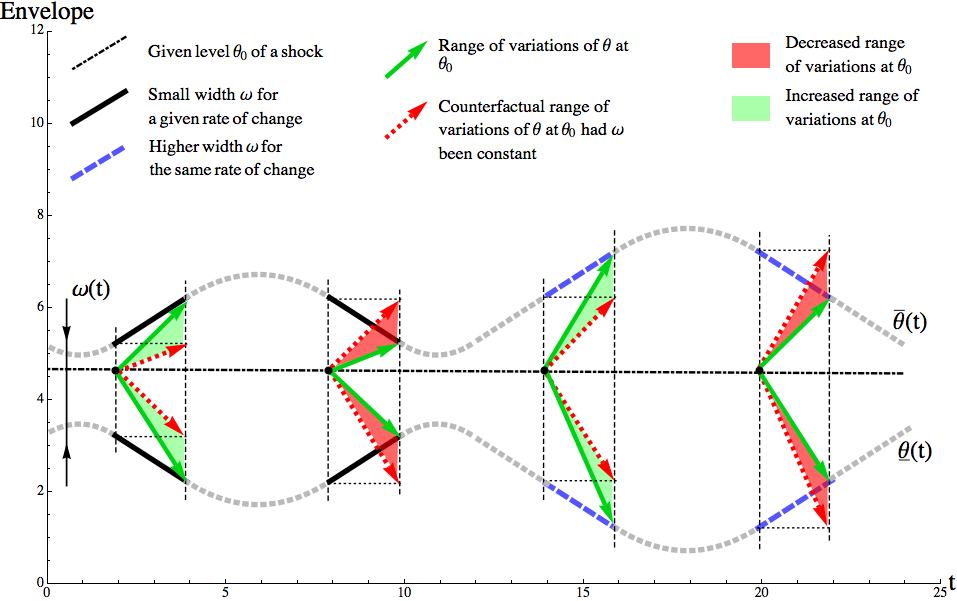
\includegraphics[width=15cm]{figch1/figdyn1.png}
\caption{\small{This graph plots an envelope of constant average value but varying width $\omega(t)$. By comparing regions of increasing or decreasing width, respectively the left or right side of a lobe, one sees that the informativeness of the envelope is being respectively reduced or increased with respect to a situation where the width would be kept constant. The change in informativeness is represented by the area between the (full) green arrows (observed level of informativeness) compared to the area between the (dashed) red arrows (level of informativeness had the width been constant). In addition, by comparing the left lobe to the right one, it is possible to see why the relative variation of the width, and not the absolute variation of the width, matters. For a larger width (right lobe) and the same rate of change in the width, there is less change in informativeness than for a smaller width (left lobe), i.e. the same rate of change matters less for the right lobe than for the left lobe. }} \label{figdyn1}
\end{figure}

All of this reasoning applies to the dynamic oligopoly result as well as the effect can be understood in the same way as for the monopoly : changes in the width of the shock's bounds behave as if there was an effective dynamic cost that was higher than the baseline when information about the shocks is lost, and lower than the baseline when information is gained.

\section{Limits}

This section aims at discussing whether or not one can consider that the mapping of these results on the real world is a set of non zero measure, to put it bluntly.\\

Further avenues of research would be to generalize our results to larger classes of demand functions. As hinted in the text of this chapter, a lot of effort has been invested towards this goal without results unfortunately. One could also solve the static case for different SDE's in order to test the sensitivity of our results on the underlying "mechanics" of the stochastic process. This has also been pursued without conclusive results : solving the optimization problem becomes quickly extremely difficult, as the second order differential equations exhibit poles, and divergences are difficult to cope with in optimization problems. \\

The nature of these avenues of research is testament to the fact that our results are obtained for a very narrow setting. However, although a healhty dose a skepticism as to the applicability of the closed form formulas is therefore warranted, I would like to argue that the results hint towards at least one more general takeaway message, namely the collapse of the set of equilibria.\\

This result stems from the nature of the mathematical problem and not from the way we set up the problem in order to maximize our chances of closed-form success per se. Therefore I think it hints towards possible more general results. The problem is the complexity of the maths as soon as one deviates from the simplest version of the problem presented here. \\

The question then becomes one of the method to employ to obtain those results. The brute force mathematical approach has proved too hard for the writer of these lines, but there is one tool that might prove useful : numerical simulations. One can solve the differential equations involved here numerically, check ex-post whether they satisfy the other conditions, and in so doing provide boundaries around possible solutions. If the unicity is a characteristic that is indeed more general than our model here, there is 0 probability of finding such a solution by the method proposed, quite literally. However providing such bounds, although not demonstrating the existence of a solution, could provide circumstantial evidence towards such a result.\\

More generally, I think that economics has not yet explored the full potential of numerical methods as a guide for theoretical results.  

\section{Discussion and Concluding Remarks}\label{ccl}

In this chapter we have introduced a supply function equilibria model of ramping costs under uncertainty.\\

By introducing technological constraints previously neglected we are able to take into account the effects of the dynamics of demand shocks on the supply function framework. We restrict ourselves to linear demand. The optimal supply schedules obtained are unique. This is a striking result when compared to traditional multiplicity of equilibria. Although we do not solve the model in the case of a general demand function (half a year was spent trying to find mathematical methods to tackle this, to no avail) we think that our results make a strong case for the reduction of the set of equilibria, in our case to a unique equilibrium, when taking into account dynamic effects, that is strategies that are history dependent. \\

We introduce a mathematical toolbox that was absent from this litterature in the past, and notably classes of stochastic differential equations that can be used to pick and choose processes yielding specific closed form distributions of probability of shocks at equilibrium. \\

Our methodology further introduces the notion of time-scale separation to our problem, which allows to transcribe quite simply static solutions to the case of dynamic envelopes of shocks, as long as the static case is solved for the same functionnal form of stochastic processes. In our case we focus our study to quadratic distributions, which we then extend to cope with any functional form for the time dependency of the envelope of shocks.\\

Our results are congruent with the economic intuition one can have about ramping costs : when they increase, the slope of the supply schedule increases in order to reduce the range of variation in production for a given range of variation of demand shocks.\\

Although mathematically more demanding than the traditional model by Klemperer and Meyer, we consider that this new model, while conceptually sparing (we only add ramping costs) allows for a richer, more realistic description of the electricity market, and opens new research avenues.  It yields precise and testable predictions on the dynamics of the electricity market with tractable functional forms, at least in the linear demand case. \\

In addition, by explicitly modeling the dynamics, our work opens the possibility to explore interactions between intraday and day-ahead markets, markets that were indistinguishable in the previous framework : if solutions are ex post optimal, there is no need to create a second type of spot market, with a shorter time horizon, the bids of the previous day should suffice. \\

Further avenues of research would be to generalize our results to larger classes of demand functions. As hinted in the text of this chapter, a lot of effort has been invested towards this goal without results unfortunately. One could also solve the static case for different SDE's in order to test the sensitivity of our results on the underlying "mechanics" of the stochastic process. This has also been pursued without conclusive results : solving the optimization problem becomes quickly extremely difficult, as the second order differential equations exhibit poles, and divergences are difficult to cope with in optimization problems.\\

Finally, and more generally, we think that this concept of ramping costs, the fact that change is costly, is ubiquitous and could fuel interesting research into the dynamics of a large range of markets. Such avenues have been pursued in the case of stochastic optimal control, that is, instantaneous reactions to stochastic shocks. Here we are describing a market on which agents are forced to optimize in advance, so that they have to react to continuous changes in the anticipated shocks, but not the shocks themselves, which can be understood as stochastic optimization with periodic commitment. 

%\bibliographystyle{te}
%\bibliography{biblio}

\begin{subappendices}
\section*{Appendix}
\addcontentsline{toc}{chapter}{Appendix}
\numberwithin{figure}{section}
\numberwithin{equation}{section}

\section{Proof of equation \ref{markovtimedep}}\label{stochasticdyn_proof}
We are here going to detail how we obtain the result in equation \ref{markovtimedep} on which the proofs of our dynamic results rely heavily. Recall that we are computing the continuous time limit of our ramping cost term which can be quite simply defined in the case of discrete dynamics but for which one has to work a bit more in order to cope with the non differentiable nature of stochastic processes. \\

We are therefore going to first consider the discrete case of a random walk of timestep $\Delta t$ which converges towards the It\={o} process \ref{sdegen}, using the Euler-Maruyama approximation, a generalisation of the Euler method to stochastic differential equations. We consider a Markov chain $Y$ defined as follows : 

\begin{equation}
\Delta Y_n=Y_{n+1}-Y_n= \mu(Y_n,n \Delta t)\Delta t+\sigma (Y_n,n \Delta t)\Delta B_n
\end{equation}


We want to derive the following : 
\begin{footnotesize}
\begin{eqnarray}
\lim_{\Delta t \to 0}\mathbb{E}\left[\frac{\Gamma(\Delta t)}{2}\left(\frac{\Delta S_i(p(\theta(t),t),t)}{\Delta t}\right)^2\middle \vert \theta(t)  \right] &=& \frac{\gamma}{2} (\partial_1S(p(\theta(t),t),t)\partial_1p(\theta(t),t))^2 \sigma(\theta,t)^2
\end{eqnarray}
\end{footnotesize}

Let us first compute the first order expansion of $\Delta S_i(p(Y_n,n\Delta t),n \Delta t)$, by assuming that both $S_i$ and $p$ are continuously differentiable with respect to their arguments:
\begin{small}
\begin{eqnarray}
\Delta S_i(p(Y_n,n\Delta t),n \Delta t) &=& \frac{\Delta S_i}{\Delta p}\left( \frac{\Delta p}{\Delta Y}\frac{\Delta Y}{\Delta t}\Delta t+ \frac{\Delta p}{\Delta t}\Delta t\right) + \frac{\Delta S_i}{\Delta t}
\Delta t +\mathcal{O}(\Delta t^2)
 \end{eqnarray}
 \end{small}
Using our differentiability assumption, note that the terms that do not depend on $\Delta Y$ scale with $\Delta t$, and that the term depending on $\Delta Y$ cannot be grouped in the same way, due to its stochastic nature, therefore:
\begin{small}
\begin{eqnarray}
\frac{\Delta S_i(p(Y_n,n\Delta t),n \Delta t) }{\Delta t} &=& \frac{\Delta S_i}{\Delta p} \frac{\Delta p}{\Delta Y}\frac{\Delta Y}{\Delta t}+\mathcal{O}(1)\\
 \left(\frac{\Delta S_i(p(Y_n,n\Delta t),n \Delta t)}{\Delta t}\right)^2 &=& \left(\frac{\Delta S_i}{\Delta p} \frac{\Delta p}{\Delta Y}\frac{\Delta Y}{\Delta t}\right)^2+ C\cdot \frac{\Delta S_i}{\Delta p} \frac{\Delta p}{\Delta Y}\frac{\Delta Y}{\Delta t} + \mathcal{O}(1)
 \end{eqnarray}
 \end{small}
 with $C$ a term that does not depend on $\Delta Y$ or $\Delta t$.\\
 
Now by considering the specification of our stochastic process we know that $\mathbb{E}\left[\frac{\Delta Y}{\Delta t}\vert Y_n\right]=\mu(Y_n,n \Delta t)$ and that $\mathbb{E}\left[\frac{\Delta Y}{\Delta t}^2 \right\vert Y_n]=\mu(Y_n,n \Delta t)^2 + \frac{\sigma (Y_n,n \Delta t)^2}{\Delta t}$. 
Using the fact that $\Gamma(\Delta t) = \gamma \Delta t + o(\Delta t)$ we obtain the result of equation \ref{markovtimedep}.


\section{Proof of Proposition \ref{monopequilibria} \label{annexmonop}}
Define the following Hamiltonian: 
\begin{equation}
\begin{split}
H(p(\theta),\dot{p}(\theta),\mu(\theta),\theta)= f(\theta)\bigg( p(\theta)(a\theta+b-p(\theta))-\frac{\lambda}{2}(a\theta+b-p(\theta))^2\\
-\frac{\gamma}{2}(1-\theta^2)\left(a-u(\theta)\right)^2\bigg)+\mu(\theta) u(\theta)
\end{split}
\end{equation}
where $u(\theta)$ is the control variable defined through the following equation of motion: $u(\theta)=\dot{p}(\theta)$, $u(\theta)\in[0,a]$. We do not consider the non-negative demand constraint and will check ex-post that our solution verifies this condition. \\

Now note that:
\begin{eqnarray}
\forall\theta\in(-1,1),&\displaystyle{\frac{\partial^2 H}{\partial p^2}}=-(2+\lambda)f(\theta)<0\label{concmono1}\\
&\displaystyle{\frac{\partial^2 H}{\partial u^2}}=-\gamma(1-\theta^2)f(\theta)<0\label{concmono2}
\end{eqnarray}
The Hamiltonian is therefore strictly concave in $p(\theta)$ and $u(\theta)$. Let $(p^*(\theta),u^*(\theta))$ be an admissible pair to the problem, that is a pair such that $u^*(\theta)=\dot{p}^*(\theta)$. If there exists a continuous and piecewise continuously differentiable function $\mu(\theta)$ such that: 
\begin{flalign}
\dot{\mu}(\theta)=-\frac{\partial H}{\partial p}^*\hspace{1.65cm}\label{mupmonop}\\
\mu(-1)=\mu(1)=0 \hspace{1.13cm}& \textrm{in order for prices to be free at the boundaries}\label{monopbound}\\
\forall (\theta,u)\in[-1,1]\times[0,a],\hspace{0.17cm}& \frac{\partial H}{\partial u}^*(u^*(\theta)-u)\geq0\label{mangaham}
\end{flalign}
with $\frac{\partial H}{\partial u}^*=\frac{\partial H}{\partial u}(p^*(\theta),u^*(\theta),\mu(\theta),\theta)$, then the Mangasarian sufficiency theorem ensures that $(p^*(\theta),u^*(\theta))$ is the optimal solution \cite[p.105]{constraint}. Let us check that eq.~\ref{monopsol} defines the optimal solution.\\

Equation \ref{mupmonop} defines $\mu(\theta)$ up to a constant. Through direct integration we obtain: $$\mu(\theta)=3a\left( (2+\lambda)\frac{4\gamma+1+\lambda}{4\gamma+2+\lambda}-1-\lambda\right)(2\theta^2-\theta^4)+const.$$
This expression is symmetric in $\theta$ therefore by choosing the adequate value for the constant, we ensure that eq.~\ref{monopbound} is satisfied. The slope of the proposed $p^*$ is in $[0,a]$ therefore eq.~\ref{mangaham} requires $\frac{\partial H}{\partial u}$ to be null.  
\begin{eqnarray}
\forall \theta \in [-1,1],~ \frac{\partial H}{\partial u}=0\implies \frac{d}{d\theta}\frac{\partial H}{\partial u}=0\hspace{3.6cm}\nonumber\\
\textrm{i.e. }\displaystyle{\dot{u} (\theta)= -\frac{4\theta}{1-\theta^2}(a-u(\theta))-\frac{(1+\lambda)(a\theta+b)}{\gamma(1-\theta^2)}+\frac{(2+\lambda)p (\theta)}{\gamma(1-\theta^2)}}
\end{eqnarray}
It is straightforward to see that the proposed solution satisfies this differential equation, thus we know that $\frac{\partial H}{\partial u}$ is a constant and as $\mu(-1)=0$ it is in fact null. Lastly,  we see that $p^*(\theta)\leq a\theta +b$.\\

The proposed $p^*(\theta)$ therefore defines the unique optimal supply function, i.e. the parametrized curve $(a \theta +b-p^*(\theta),p^*(\theta))$.

\section{Proof of Proposition \ref{propoligo1} \label{annex1}}
As for eq.~\ref{maxoligopo}, for the sake of concision, we do not write the explicit depencies of the different functions on $\theta$, thus $f(\theta)$, $p(\theta)$, $u(\theta)$, $\mu(\theta)$ and $S(p(\theta))$ will be written as $f$, $p$, $u$, $\mu$ and $S$ respectively. Define the following Hamiltonian: 
\begin{equation}
\begin{split}
H(p,u,\mu,\theta)= f\bigg( p(a\theta+b-p-(n-1)S)-\frac{\lambda}{2}(a\theta+b-p-(n-1)S)^2\\
-\frac{\gamma}{2}(1-\theta^2)\left(a-u(1+(n-1)S')\right)^2\bigg)+\mu u
\end{split}
\end{equation}
where $u$ is the control variable defined through the following equation of motion: $u=\dot{p}$, $u\in[0,a]$. We do not consider the non-negative demand constraint and will check ex-post that our solution verifies this condition. \\

If a symmetric equilibria exists, eqs.~\ref{condsymi} through~\ref{condsymf} imply that the regular conditions for an admissible pair to be optimal write  :
\begin{flalign}
&u=\dot{p}\in[0,a]&\\
&\partial_uH<0\implies u=0&\\
&\partial_uH>0\implies u=a&\\
\begin{split}\partial_uH=0\implies u\in[0,a]\textrm{ and} \hspace{6cm}\\
\ddot{p}=-\frac{4\theta(a-\dot{p})}{1-\theta^2}-\frac{\lambda(a\theta+b-p)}{\gamma(1-\theta^2)}-n\frac{\dot{p}(a\theta+b-2p)-a(n-1)p}{\gamma(1-\theta^2)(a(n-1)+\dot{p})}
\end{split}\label{oligoequadiff}\\
&\dot{\mu}=-\partial_pH&\\
&\mu(-1)=\mu(1)=0&\label{oligobc}
\end{flalign}
It is easy to check that $(K_1,K_2)\in(0,1)$ and that the solution~\ref{oligosol} solves eq.~\ref{oligoequadiff} subject to the boundary conditions~\ref{oligobc}. The supply schedule is therefore also linear, with equation :
\begin{flalign}
& S(p)=\frac{1}{n}\left( p\left( \frac{1}{K_1}-1\right)+b\left( 1-\frac{K_2}{K_1}\right) \right)&\label{oligoS}
\end{flalign}
We can now use the Mangasarian theorem to obtain that our admissible pair is indeed solution, $H(p,u,\mu,\theta)$ being concave in $(p,u)$ for linear supply schedules. However the Mangasarian cannot yield that this solution is unique because for a symmetric equilibria, if supply schedules are modified, the hamiltonian changes alongside and we are faced with a new maximisation program. \\

To obtain that the solution is unique we are going to show explicitly that no other candidate solution exists. \\

First, note that :
\begin{flalign}
\begin{split}
\dot{\mu}=-f\bigg( \frac{a\theta+b-2p}{n}-a\frac{(n-1)p}{n\dot{p}}\hspace{5cm}\\
+\lambda\frac{a\theta+b-p}{n}\cdot\frac{a(n-1)+\dot{p}}{n\dot{p}}-\gamma(1-\theta^2)(n-1)\frac{a-\dot{p}}{n}\cdot\frac{a\ddot{p}}{n\dot{p}^2}\bigg)\label{oligomup}
\end{split}
\end{flalign}
If $(p^*,u^*)$ maximises the program then the maximum principle implies that there exists a continuous and piecewise continuously differentiable function $\mu$, as shown in \cite[Theorem 2 p.85]{constraint}. This combined with the above equation implies that $\dot{p}\neq0$ a.e.\\

Assume now a solution of the form $\forall\theta\in[-1,1],~p=a\theta+\beta$, by injecting this expression in eq.~\ref{oligomup} there is no $\beta$ such that  the boundary conditions~\ref{oligobc} are verified. \\

In addition:
\begin{flalign}
&\forall\theta\in(-1,1),~\displaystyle{\frac{\partial^2 H}{\partial u^2}}=-f\gamma(1-\theta^2)(1+(n-1)S')^2<0\label{concoligo}&
\end{flalign}
The Hamiltonian is therefore strictly concave in $u$ and $[0,a]$ is convex. These two properties yield that $u^*$ is continuous, as shown in \cite[Note 2.b. p.86]{constraint}. We have proved the following result :
\begin{lemma}
For any symmetric equilibrium $\exists A\subseteq[-1,1]$ s.t. A is the union of segments of $[-1,1]$ and $\forall\theta\in A$, $\partial_u H=0$ 
\end{lemma}

Assume the following hypothesis is true, $H_1:\exists\theta_c\in(-1,1)$ s.t. $[-1,\theta_c]\subseteq A$, then knowing that $\dot{p}\in\mathcal{C}^0([-1,1],[0,a])$ we can rewrite differential equation \ref{oligoequadiff} around the value $\theta=-1$ by defining $\theta=-1+\epsilon$ with $\epsilon=o(1)$:
\begin{flalign}
&\frac{d^2p}{d\epsilon^2}= \frac{C}{\epsilon}+o(1) \textrm{ with }C\neq0 \textrm{ if }p(\theta)\neq aK_1\theta+bK_2&
\end{flalign}
This means that locally around $-1$, any solution to eq. \ref{oligoequadiff} but solution \ref{oligosol} diverges. Hypothesis $H_1$ is therefore wrong and $\exists\theta_c\in(-1,1)$ s.t. $\forall\theta\in[-1,\theta_c]$, $\exists \beta$ s.t. $p(\theta)=a\theta+\beta$.\\

At $\theta_c$ we have $\partial_u H=0$ and as $\dot{p}$ is continuous, $\dot{p}(\theta_c)=a$. For the solution to be interior we need $\ddot{p}(\theta_c)\leq0$. 
\begin{flalign}
&\partial_{\dot{p}}H(p,\dot{p},\mu,\theta_c)=0\Leftrightarrow \mu(\theta_c)=0&\\
&\ddot{p}(\theta_c)\leq0\Leftrightarrow b(1+\lambda)-\beta(n+1+\lambda)\geq na\theta&
\end{flalign}
Straightforward computations show that both conditions are mutually exclusive, therefore there doesn't exist another candidate symmetric equilibria, and our solution is unique.\\

Lastly, to compute the optimal supply function, we inverse the optimal price in order to get the shock as a function of the price at the equilibrium, and we inject this expression in Eq. \ref{supequ}.

\section{Proof of proposition \ref{oligoslope_prop}}\label{oligopslope_proof}
We want to prove that the slope of the supply schedules increases as the ramping cost parameter increases. As a reminder:
\begin{flalign}
&\displaystyle{K_1=\frac{n\sqrt{(4\gamma+\lambda+n)^2-4n+4}-(4\gamma+\lambda+n)(n-2)}{2(4\gamma+\lambda+2n)}}& \\
&\displaystyle{K_2=\frac{\lambda(n-1)+K_1(\lambda+n)}{(\lambda+n)(n-1)+K_1(\lambda+2n)}}&
\end{flalign}
and the supply schedule has the following expression:
\begin{flalign}
&S^*(p)=\frac{1}{n}\left( p\left( \frac{1}{K_1}-1\right)+b\left( 1-\frac{K_2}{K_1}\right) \right)&
\end{flalign}
Let us study how $K_1$ varies with $\gamma$. Note first that if one defines $G=4\gamma+\lambda+n$, then $\frac{\partial K_1}{\partial \gamma} =\frac{\partial K_1}{\partial G} \frac{\partial G}{\partial \gamma} = 2\frac{\partial K_1}{\partial G}$. 

therefore the sign of  $\frac{\partial K_1}{\partial \gamma}$ is given by that of:
\begin{small}
\begin{flalign}
&\frac{\partial K_1}{\partial G} = \frac{\partial}{\partial G}\left[\frac{n\sqrt{G^2-4n+4}-G(n-2)}{2(G + n)}\right]& \\
&= \frac{(\sqrt{G^2-4n+4})((G+n)(nG-(n-2)\sqrt{G^2-4n+4})-(n\sqrt{G^2-4n+4}-G(n-2)))}{4(G+n)^2}&\\
&= \frac{(\sqrt{G^2-4n+4})(n^2G+4n^2-4n - n(n-2)\sqrt{G^2-4n+4})}{4(G+n)^2}&\\
&=  \frac{(\sqrt{G^2-4n+4})(2G+4+(n-2)(G+4-\sqrt{(G+4)^2-8G-4n-12}))}{4(G+n)^2}>0&
\end{flalign}
\end{small}

Therefore $\frac{\partial S^*(p)}{\partial\gamma}<0$ which implies that schedules see their slope increase with $\gamma$ in the plane $(q,p)$.\\

We can perform the same type of computation for the ratio $\frac{K_2}{K_1}$, using the fact that $\partial_\gamma K_1>0$:
\begin{small}
\begin{flalign}
&\frac{\partial K_2/K_1}{\partial \gamma} = -\frac{\partial_\gamma K_1(K_1^2(\lambda+2n)(\lambda+n)+2 K_1(\lambda+2n)(n-1)\lambda + \lambda(\lambda+n)(n-1)^2)}{K_1^2((\lambda+n)(n-1)+K_1(\lambda+2n))^2}<0& 
\end{flalign}
\end{small}
This implies that the schedule is shifted to the right in the plane $(q,p)$ when ramping costs increase.  

\section{Proof of proposition \ref{monopropdyn}}\label{monopdyn_proof}

Define the following Hamiltonian: 
\begin{equation}
\begin{split}
H(p(\theta,t),\dot{p}(\theta,t),\mu(\theta,t),\theta,t)= f(\theta,t)\bigg( p(\theta,t)(\theta-p(\theta,t))-\frac{\lambda}{2}(\theta-p(\theta,t))^2\\
-\frac{\gamma}{2}\sigma(theta,t)^2\left(1-u(\theta,t)\right)^2\bigg)+\mu(\theta,t) u(\theta,t)
\end{split}
\end{equation}
where $u(\theta,t)$ is the control variables defined through the following equation of motion: $u(\theta,t)=\dot{p}(\theta,t)$, $u(\theta,t)\in[0,1]$. \\

Note that the methods used previsouly generalise to multi-dimensional problems, and that here, our problem depends on $\theta$ and $t$ instead of only $\theta$ as in the case of the static monopoly problem. \\

Further note that the problem does not depend on the time derivative of $p(\theta,t)$. This means that what would be a general Euler-Lagrange formulation expressed as $\frac{\partial\mathcal{L}}{\partial p} - \frac{\partial}{\partial \theta}\frac{\partial \mathcal{L}}{\partial \dot{p}} - \frac{\partial}{\partial t}\frac{\partial \mathcal{L}}{\partial \partial_t p}$, which is the equation that has to be solved for interior solutions, reduces to  $\frac{\partial\mathcal{L}}{\partial p} - \frac{\partial}{\partial \theta}\frac{\partial \mathcal{L}}{\partial \dot{p}}$, where  $\mathcal{L}(t,\theta,p,\dot{p}) = H(p,\dot{p},0,\theta,t)$. This is the exact same problem as before, with the only addition that our parameters now vary with $t$, but the partial differential equation is the same one as before. \\

Therefore the problem can be solved exactly as before by replacing the variance term by its new dynamic version, that is that it is as if the ramping cost parameter $\gamma$ was replaced by $\gamma \cdot \left( 1+ \frac{\tau}{\omega}\frac{d\omega}{dt}\right)$ in the static solution.\\

This can be seen by noting that $\sigma(\theta,t)^2 = \left(1+\frac{\tau}{\omega}\frac{d\omega}{dt}\right)(\theta-\hat{\theta}+\omega)(\hat{\theta}+\omega-\theta)$ which has to fall back to the static case in the limit, therefore we see that we simply get an additional $\left(1+\frac{\tau}{\omega}\frac{d\omega}{dt}\right)$ term that appears on the ramping cost term, that is that multiplies $\gamma$.

\section{Proof of proposition \ref{oligodynp}}\label{oligodyn_proof}

The exact same reasoning as the one in Annex \ref{monopdyn_proof} applies here and we only have to take our static oligopoly result and replace  $\gamma$ by $\gamma \cdot \left( 1+ \frac{\tau}{\omega}\frac{d\omega}{dt}\right)$ to obtain the dynamic results.













%\section{Stochastic process} \label{rampingcostsappendix}
%
%\subsection{The ramping costs}
%In the rest of the paper we are going to consider quadratic ramping costs. More precisely we consider the costs induced by fluctuations in the production level. As described in the introduction, fluctuations imply increased wear and tear, whether the production is increasing or decreasing. In addition, these ramping costs are null in the absence of fluctuations. This means that they can be captured by a function $C_r(\cdot)$ verifying $C_r(0)=0$, $C_r(\cdot)\geq0$ and increasing in the absolute value of its argument. In the abscence of more detailed knowledge about the actual shape of these ramping costs, it seems reasonable to consider a quadratic cost function, that is the first term in a Taylor expansion of the actual real ramping cost function. \\
%
%We cannot compute $\frac{d\theta}{dt}$ as it appears in Eq.~\ref{maxbase}, as a stochastic process, although everywhere continuous, is nowhere differentiable. We are therefore going to consider a random walk of timestep $\Delta t$ which converges towards the It\={o} process \ref{sdegen}, using the Euler-Maruyama approximation, a generalisation of the Euler method to stochastic differential equations. We consider a Markov chain $Y$ defined as follows : 
%
%\begin{equation}
%\Delta Y_n=Y_{n+1}-Y_n= \mu(Y_n,n \Delta t)\Delta t+\sigma (Y_n,n \Delta t)\Delta B_n
%\end{equation}
%where $\Delta B_n=B_{(n+1)\Delta t}-B_{n\Delta t}$. These $\Delta B_n$ are \emph{i.i.d.} normal random variables of mean $0$ and variance $\Delta t$. Note that as $\Delta t$ is taken towards $0$, this Markov chain converges towards its underlying stochastic process defined by eq.(\ref{sdegen}).\\
%
%The ramping costs are taken as quadratic in the variation of the production, so we compute the following quantity : 
%
%\begin{equation}
%\mathbb{E}\left[\left(\frac{Y_{n+1}-Y_n}{\Delta t}\right)^2\middle \vert Y_n  \right]=\frac{\sigma (Y_n,n \Delta t)^2}{\Delta t}
%\label{markovariation}
%\end{equation}
%
%which obviously diverges when the Markov chain is taken towards its underlying stochastic process. To overcome this issue we have to consider a technological constraint : below a given timescale, power plants do not face ramping costs anymore. Two distinct mechanisms justify this statement, both induced by the very nature of the ramping costs : wear and tear is due to the fluctuations of temperature in the core of the power plant. \\
%
%The first mechanism through which ramping costs disappear below a given timescale is that for fluctuations occurring on the typical timescale of the millisecond and below, the production does not actually fluctuate. If the consumption varies very rapidly, the frequency of the electric network automatically adjust, thus it is not even asked of the production to change. \\
%
%The second mechanism through which ramping costs vanish below a given timescale is that for fluctuations occurring on the typical timescale of the second and below, although the production does fluctuate, the temperature in the core of the power plant does not. This comes form the thermal inertia of the materials forming the power plant. Fluctuations of consumption on these typical timescales, if they do imply a change in production, do not change the temperature in the core, and consequently do not imply ramping costs. This can be understood by using an everyday life analogy : lighting a stove is extremely quick, but the water being heated will take time to boil, because of its thermal inertia. \\
%
%Those two mechanisms effectively act as low-pass filters between the consumption on the network and the temperature in the core of the power plant, which bounds from below the timestep of the Markov process. In both cases, the typical timescales below which fluctuations become irrelevant (milliseconds or seconds), which we call the cutoff timescale $\Delta t_c$, are much smaller than the typical timescales of the change in strategies that we are trying to explain (hour). \\
%
%The ramping costs are written as a function of the production for convenience, although the fact that they actually depend on the temperature of the core is used to explain the existence of a cutoff timescale. We consider a Markov chain converging towards a stochastic process. From eq.(\ref{markovariation}) we see that this approach leads to diverging ramping costs, and that the cutoff timescale allows for a technologically driven argument for which these costs are actually finite.  \\
%
%Consider a transformation $T(\cdot)$ that we apply to the Markov chain $Y$. Then:
%\begin{equation}
%\mathbb{E}\left[\left(\frac{T(Y_{n+1})-T(Y_n)}{\Delta t}\right)^2\middle \vert Y_n  \right]= \mathbb{E}\left[\left(\frac{T(Y_{n+1})-T(Y_n)}{Y_{n+1}-Y_n}\cdot\frac{Y_{n+1}-Y_n}{\Delta t}\right)^2\middle \vert Y_n  \right]    
%\label{markovcomposed}
%\end{equation}
%
%And in the limit:
%\begin{equation}
%\lim_{\Delta t \to 0}\mathbb{E}\left[\left(\frac{T(Y_{n+1})-T(Y_n)}{\Delta t}\right)^2\middle \vert Y_n  \right]= T'(Y_n)^2 \lim_{\Delta t \to 0}\mathbb{E}\left[\left(\frac{Y_{n+1}-Y_n}{\Delta t}\right)^2\middle \vert Y_n  \right]    
%\label{limitmarkovcomposed}
%\end{equation}
%But here, the right hand side diverges. We consider that $\Delta t_c$ is sufficiently small to justify the final approximation we are going to make in order to describe properly the problem at hand. We assume that the ramping cost function, considering a generic shock process $\theta(t)$ of the type given in eq.(\ref{sdegen}), can be written as: 
%\begin{equation}
%\mathbb{E}\left[\left(\frac{\Delta S_i(p(\theta(t)))}{\Delta t_c}\right)^2\middle \vert \theta(t)  \right] = \mathbb{E}\left[\left(\frac{\Delta S_i(p(\theta(t)))}{\Delta \theta(t)} \frac{\Delta \theta(t)}{\Delta t_c}\right)^2\middle \vert \theta(t)  \right]  \approx S_i'(p(\theta(t)))^2\dot{p}(\theta(t))^2 \frac{\sigma(\theta)^2}{\Delta t_c}
%\label{markovtosde}
%\end{equation}
%with $X'$ the derivative of quantity X with respect to its argument, $\dot{X}$ its derivative with respect to $\theta$ and $\Delta X(t)=X(t+\Delta t_c)-X(t)$. This is equivalent to saying that $\Delta t_c$ is sufficiently small to approximate these increase rate of the supply and price functions by their derivatives, i.e. do a first order taylor expansion. Note that we considered here that the variance term $\sigma$ depends only on $\theta$ and not explicitly on $t$, which in turn implies that the strategy $S_i$ does not depend explicitly on $t$ either. \\
%
%Let us consider the case where the strategy and the variance depend explicitly on the time, and are thus written $S_i(p(\theta(t)),t)$ and $\sigma(\theta,t)$ respectively.  By using a first order expansion as before, the ramping cost function can be approximated as follows:
%\begin{eqnarray}
%\mathbb{E}\left[\left(\frac{\Delta S_i(p(\theta(t)),t)}{\Delta t_c}\right)^2\middle \vert \theta(t)  \right] &\approx& \partial_1S_i(p(\theta(t)),t)^2\dot{p}(\theta(t))^2 \frac{\sigma(\theta,t)^2}{\Delta t_c} +\partial_2 S_i(p(\theta(t)),t)^2\nonumber\\
%&&+2\partial_1S_i(p(\theta(t)),t)\partial_2 S_i(p(\theta(t)),t) \dot{p}(t)\mathbb{E}\left[\frac{\Delta \theta(t)}{\Delta t_c}\middle \vert \theta(t)  \right]
%\label{markovtimedep}
%\end{eqnarray}
%with $\partial_iX$ the partial derivative of quantity $X$ with respect to its $i^{th}$ argument. We are now going to develop an argument that we made earlier: $\Delta t_c $ is considered much smaller (millisecond to seconds) than the typical timescale of change in strategies we are trying to capture (hour). This directly justifies the fact that we are going to neglect the second and third terms in the right hand side of eq.(\ref{markovtimedep}). We consider that:
%\begin{equation}
%\mathbb{E}\left[\left(\frac{\Delta S_i(p(\theta(t)),t)}{\Delta t_c}\right)^2\middle \vert \theta(t)  \right]  \approx \partial_1S_i(p(\theta(t)),t)^2\dot{p}(\theta(t))^2 \frac{\sigma(\theta,t)^2}{\Delta t_c}
%\label{finalapprox}
%\end{equation}
%
%Now, we can write down the instantaneous expected value of the profit of producer $i$ if the demand shock is $\theta(t)$, $\pi^e_i(t)$, that is the profit that one expects to obtain when demand is at $\theta(t)$ given the expected value of the ramping costs:
%
%\begin{equation}
%\pi^e_i(t)= p(\theta(t))S_i(p(\theta(t)),t) - C_s(S_i(p(\theta(t)),t)) -\frac{\gamma_0}{2} \partial_1S_i(p(\theta(t)),t)^2\dot{p}(\theta(t))^2 \frac{\sigma(\theta,t)^2}{\Delta t_c}
%\label{instantprofit}
%\end{equation}
%
%Lastly we have to write down the expected profit for a day's worth of submitted strategies. Let us consider that the chosen unit of time is the day. Therefore, the total expected profit $\Pi^e_i$ writes: 
%
%\begin{eqnarray}
%\Pi^e_i&=&\int_0^1\mathbb{E}[\pi^e_i(t)]dt\nonumber\\
%&=&\int_0^1\int_{\underline{\theta}}^{\overline{\theta}}f(\theta,t)\left[p(\theta)S_i(p(\theta),t) - C_s(S_i(p(\theta),t)) -\frac{\gamma}{2} \partial_1S_i(p(\theta),t)^2\dot{p}(\theta)^2 \sigma(\theta,t)^2\right]d\theta dt
%\label{totprofit}
%\end{eqnarray}
%with $\gamma=\gamma_0/\Delta t_c$
%
%\subsection{Discussion of the approximations}
%We want a tractable mathematical formulation of the dynamic problem faced by producers on the electricity market. To achieve this we seek to describe the discrete real life problem by an approximated continuous one. We first use two technological facts: fluctuations in production are costly, but only up to a certain cutoff timescale.  We note that this cutoff timescale is much smaller than the typical timescale of the dynamics we try to capture. We then use two types of mathematical approximations. The first one is that we rely heavily on first order expansions of the different terms we have to compute. The second one stems from the existence of these two different timescales that allow us to neglect certain terms but not others in these first order expansions. From the very beginning of this work, we build a framework aimed at capturing the dynamics of the market and exploit some technological constraints in order to make simplifications. The consequence of this modelling strategy is that this model, by construction, will not be able to adress very short term economic questions. 
%
%\subsection{The maximisation program}
%Here, we consider that the dynamics of demand shocks are given by eq.(\ref{eqSDE}), and that therefore  $\sigma(\theta,t)^2=\sigma(\theta)^2=(1-\theta^2)$.\\
%
%We now introduce the different conditions that have to be satisfied by the various terms in this problem. First, on most electricity markets, schedules must be increasing, therefore here we take $S_i'(\cdot)\geq0$. Second, the aggregate demand is non negative as consumers do not have production facilities at their disposal: $D(\theta(t),p(\theta(t)))=\sum_iS_i(p(\theta(t)))\geq0$. Last, we consider that the shocks $\theta$ are ordered so that the demand is increasing in $\theta$, i.e. $\frac{\partial D}{\partial\theta}\geq0$, and that the price has to weakly increase with the shocks, i.e. $\dot{p}\geq0$. Our initial stochastic maximisation program can thus be rewritten as a regular optimal control problem: 
%
%\begin{equation}
%\displaystyle{\max_{S_i(p)}}~\int_{-1}^{1} f(\theta)\left(p(\theta)S_i(p(\theta)) -C_s(S_i(p(\theta)))-\frac{\gamma}{2}(1-\theta^2)\left(S_i'(p(\theta))\dot{p}(\theta)\right)^2\right)d\theta
%\end{equation}
%\begin{eqnarray} 
%s.t.\hspace{2cm}&S_i'(\cdot)\geq0 \nonumber\\
%&\dot{p}\geq0\\
%&D(\cdot,\cdot)\geq0 \nonumber\\
%\end{eqnarray}
%
%The next section solves this problem for a monopoly. 

%\subsection{Link between residuals and width}\label{reswidth}
%
%Here I compute the range of production that can be realised at a given time $t$.
%
%Extremal demand functions : $D_{extr}(p)=b\pm a-p$. At the equilibrium, the supply function obtained in Eq. \ref{dynsupply} must be equal to the demand. Therefore the extremal equilibrium points are obtained from the following equation :
%
%\begin{eqnarray}
%\frac{1}{n}\left( p^*_{extr}\left( \frac{1}{K_1(t)}-1\right)+\hat{\theta}\left( 1-\frac{K_2(t)}{K_1(t)}\right) \right)=b\pm a-p^*_{extr}\\
%p^*_{extr}=\frac{nK_1(t)(b\pm a)+\hat{\theta}(K_2(t)-K_1(t))}{1+(n-1)K_1(t)}
%\end{eqnarray}
%Therefore we can compute the extremal production values:
%\begin{eqnarray}
%\frac{1}{n}\left( p^*_{extr}\left( \frac{1}{K_1(t)}-1\right)+\hat{\theta}\left( 1-\frac{K_2(t)}{K_1(t)}\right) \right) =\frac{K_1(t)}{1+(n-1)K_1(t)}\left( b\pm a +\hat{\theta}\left( 1-\frac{K_2(t)}{K_1(t)}\right)\right)
%\end{eqnarray} 
%Define $\Delta Q(t)$ as the range of possible quantities produced. Then
%\begin{equation}
%\Delta Q(t)=\frac{2aK_1(t)}{1+(n-1)K_1(t)}
%\end{equation}
%Now we can ask how does this range, which is correlated with the absolute value of the error termes between predicted production and realised production, changes in time.
%\begin{eqnarray}
%\frac{d \Delta Q(t)}{dt}=\frac{\frac{d K_1(t)}{dt}}{(1+(n-1)K_1(t))^2}
%\end{eqnarray} 
%This quantity is of the sign of $\frac{d K_1(t)}{dt}$. For concision, note $\frac{1}{\omega}\frac{d\omega}{dt}=\frac{\omega'}{\omega}$ with $X'=\frac{dX}{dt}$
%\begin{equation}
%\frac{d K_1(t)}{dt}=\frac{2 \gamma  n \left(\frac{\omega'}{\omega}\right)' \left(n^2-4+n (4 \gamma(1+\frac{\omega'}{\omega}) +\lambda+4)-(n-2) \sqrt{(4 \gamma  (1+\frac{\omega'}{\omega})+\lambda +n)^2-4 n+4}\right)}{(4 \gamma(1+  \frac{\omega'}{\omega}) +\lambda +2 n)^2 \sqrt{(4 \gamma  (1+\frac{\omega'}{\omega})+\lambda +n)^2-4 n+4}}
%\end{equation}
%Thus, $sign\left(\frac{d \Delta Q(t)}{dt}\right)=sign\left(\frac{\omega'}{\omega}\right)'$
%$$\Delta Q=\frac{\omega K_1}{1+(n-1)K_1}$$\tiny
%$$\frac{d\Delta Q}{dt}=\frac{\omega'(t) \left(n \sqrt{\left(4 \gamma +\lambda +n+\frac{4 \gamma  \omega'(t)}{\omega(t)}\right)^2-4 n+4}+(2-n) \left(4 \gamma +\lambda +n+\frac{4 \gamma  \omega'(t)}{\omega(t)}\right)\right) \left(4 \gamma +\lambda +2 n+\frac{4 \gamma  \omega'(t)}{\omega(t)}\right)+\frac{4 \gamma  \left(\omega(t) y''(t)-\omega'(t)^2\right) \left(\frac{n \left(4 \gamma +\lambda +n+\frac{4 \gamma  \omega'(t)}{\omega(t)}\right)}{\sqrt{\left(4 \gamma +\lambda +n+\frac{4 \gamma  \omega'(t)}{\omega(t)}\right)^2-4 n+4}}-n+2\right) \left(4 \gamma +\lambda +2 n+\frac{4 \gamma  \omega'(t)}{\omega(t)}\right)}{\omega(t)}-\frac{4 \gamma  \left(\omega(t) y''(t)-\omega'(t)^2\right) \left(n \sqrt{\left(4 \gamma +\lambda +n+\frac{4 \gamma  \omega'(t)}{\omega(t)}\right)^2-4 n+4}+(2-n) \left(4 \gamma +\lambda +n+\frac{4 \gamma  \omega'(t)}{\omega(t)}\right)\right)}{\omega(t)}}{2 \left(4 \gamma +\lambda +2 n+\frac{4 \gamma  \omega'(t)}{\omega(t)}\right)^2}$$












%\newpage
%\subsection{Symmetric oligopoly with general demand and cost functions}
%Assume that the inertial cost function has the property that $C_i(A\cdot B)=C_i(A)\cdot C_i(B)$, that is $C_i$ is a power function, or, more generally, consider any analytical function on $\mathbb{R}$, and as before, $\dot{X}=\frac{dX}{d\theta}$. Given a price $p(t)$ at date $t$, the instantaneous profit can be written as : 
%\begin{equation}
%\begin{split}
%\Pi(t)=p(t)\big[D(\theta(t),p(t)) -(n-1)S(p(t)) \big]-C_s\big(D(\theta(t),p(t)) -(n-1)S(p(t)) \big)\\
%-C_i\big(\dot{D}(\theta(t),p(t)) -(n-1)S'(p(t))\dot{p}(t) \big)C_i\bigg( \frac{d\theta}{dt}\bigg)
%\end{split}
%\end{equation}
%
%Demand is decreasing with price and we can always redefine and reorder the shocks so that demand is increasing with shocks: $\partial_p D\leq0$ and  $\partial_\theta D\geq0$. Along the equilibrium, we consider that the total production is weakly increasing in the shocks: $\dot{D}\geq0$. Lastly the price itself is weakly increasing in the shocks, so that $\dot{p}\geq0$. These two conditions can be summarized as $\dot{p}\in[0,-\frac{\partial_\theta D}{\partial_p D}]$ and lastly total production is always positive: $D\geq0$. Define $C_I(\theta,t)=\mathbb{E}\bigg[ C_i\bigg(\displaystyle{\frac{d\theta}{dt}}\bigg)\bigg|\theta,t \bigg]$. \\
%
%Let us start from the situation where the first $n-1$ producers bid the same supply function $S$. The maximization program of the $n^{th}$ producer writes:
%\begin{equation}
%\begin{split}
%\max_{p(\theta,t)}\int_{-1}^1 f(\theta,t)\bigg[ p\big[D(\theta,p) -(n-1)S(p) \big]
%-C_s\big(D(\theta,p) -(n-1)S(p) \big)\\
%-C_i\big(\dot{D}(\theta,p) -(n-1)S'(p)\dot{p} \big)C_I( \theta,t)\bigg]d\theta
%\end{split}
%\end{equation}
%s.t.
%\begin{flalign}
%&\dot{p}\in\left[0,-\frac{\partial_\theta D}{\partial_p D}\right]&\\
%&D\geq0&
%\end{flalign}
%
%
%
%
%
%\newpage
%At the symmetric equilibria we know that:
%\begin{flalign}
%&nS(p)=D(\theta,p) &\\
%&S'(p)=\frac{\dot{D}}{n\dot{p}}=\frac{\partial_\theta D+\partial_p D\dot{p}}{n\dot{p}}&\\
%&S''(p)=\frac{\ddot{D}\dot{p}-\dot{D}\ddot{p}}{n\dot{p}^2}=\frac{\dot{p}\partial_{\theta\theta}D+2\dot{p}^2\partial_{p\theta}D+\dot{p}^3\partial_{pp}D -\ddot{p}\partial_\theta D}{n\dot{p}^3}&
%\end{flalign}
%
%From optimal control theory we obtain that the maximizing $p(\theta)$ is solution of the following differential equation:
%\begin{equation}
%\begin{split}
%\ddot{p}=-\frac{n}{\partial_p D}\frac{C_i'\left( \frac{\dot{D}}{n}\right)}{C_i''\left(\frac{\dot{D}}{n} \right)} \left[ \frac{\dot{f}(\theta,t)}{f(\theta,t)}+\frac{C_I'(\theta,t)}{C_I(\theta,t)}\right]-\frac{\ddot{D}}{\partial_pD}-\frac{n\left(p-C_s\left( \frac{D}{n}\right)\right)}{\partial_pD~ C_I(\theta,t)C_i''\left( \frac{\dot{D}}{n}\right)}\\
%-\frac{nD\dot{p}}{\partial_pD(\dot{p}\partial_pD-(n-1)\partial_\theta D)C_I(\theta,t)C_i''\left( \frac{\dot{D}}{n}\right)}
%\end{split}
%\end{equation}
%
%\subsubsection{Unicity}
%The same exact reasonning as in the linear case shows that the solution is completely interior. 
%For $\theta=-1$ or $\theta=1$, we obtain the following boundary conditions: 
%\begin{equation}
%\begin{split}
%0=-nC_i'\left( \frac{\dot{D}}{n}\right)\left[ \frac{\dot{f}(\theta,t)}{f(\theta,t)}+\frac{C_I'(\theta,t)}{C_I(\theta,t)}\right](\dot{p}\partial_pD-(n-1)\partial_\theta D)C_I(\theta,t)\\
%-n\left(p-C_s\left( \frac{D}{n}\right)\right)(\dot{p}\partial_pD-(n-1)\partial_\theta D)-nD\dot{p}
%\end{split}
%\end{equation}
%Unless these two conditions are "colinear" (ex. $y''=-y$ with $y(0)=0=y(2\pi)$) the solution is unique. 
%
%\subsubsection{Existence}
%\begin{equation}
%\begin{split}
%\max_{p(\cdot)}\int_{-1}^1f[p(D-(n-1)S)-C_s(D-(n-1)S)-C_i(\dot{D}-(n-1)S'\dot{p})C_I]d\theta
%\end{split}
%\end{equation}
%
%Filipov yields that there always exists a best response. If we consider the application that for any supply curve $S$ on which the $n-1$ competitors agree on outputs the BR, then we can use a fixed point argument to obtain the existence of a symmetric equilibria.












%\begin{theorem}

%\end{theorem}
%\subsection{Oligopoly solution}
%\begin{itemize}
%\item Consider that the solution is of slope $a$ everywhere and is expressed as $p(\theta)=a\theta+\beta$. Then 
%\begin{flalign}
%\begin{split}
%\dot{\mu}=-f\bigg( \frac{a\theta+b-2p}{n}-\frac{a(n-1)p}{n\dot{p}} +\lambda(a\theta+b-p)\frac{a(n-1)+\dot{p}}{n^2\dot{p}}\\
%-\gamma\frac{1-\theta^2}{n\dot{p}^2}(a-\dot{p})(n-1)a\ddot{p}\bigg)\\
%\end{split}
%\end{flalign}
%\begin{flalign}
%\dot{\mu}=\frac{3a}{4}(\theta-\theta^3)-\frac{3(1+\lambda)}{4n}(b-\beta)(1-\theta^2)
%\end{flalign}
%so that 
%\begin{flalign}
%\mu=\frac{3a}{16}(2\theta^2-\theta^4)-\frac{3(1+\lambda)}{12n}(b-\beta)(3\theta-\theta^3)+const
%\end{flalign}
%We see that $\mu$ has odd terms in $\theta$, thus $\mu(-1)\neq\mu(1)$ unless $b=\beta$, in which case  it is a solution, with $0$ profit. 
%\item We check that \emph{ad hoc} functions of the form presented in Fig.~\ref{fig:oligop}, yield positive profits, thus $p(\theta)=a\theta+b$ is not the solution.
%\item $\mu(\theta)$ is absolutely continuous thus 
%\end{itemize}
%\subsection{Assymetric duopoly}
%Assume that $S_2(p)$ is linear, i.e. $S_2(p)=\alpha_2p+\beta_2$, and $S_1(p)+S_2(p)=a\theta+b-p$.
%\begin{equation}
%\begin{split}
%\max_{p}\int_{-1}^1f\bigg( p(a\theta+b-(1+\alpha_2)p-\beta_2)-\frac{\lambda}{2}(a\theta+b-(1+\alpha_2)p-\beta_2)^2\\
%-\frac{\gamma}{2}(1-\theta^2)(a-(1+\alpha_2)\dot{p})^2\bigg)\label{duopo}
%\end{split}
%\end{equation}
%s.t. $\dot{p}\in[0,\frac{a}{1+\alpha_2}]$ and $p\leq \frac{a\theta+b-\beta_2}{1+\alpha_2}$.\\
%
%Define:
%\begin{flalign}
%&p_0=\sqrt{1+\alpha_2}p&\\
%&a_0=\frac{a}{1+\alpha_2}&\\
%&b_0=\frac{b-\beta_2}{1+\alpha_2}&\\
%&\lambda_0=\lambda(1+\alpha_2)&\\
%&\gamma_0=\gamma(1+\alpha_2)&
%\end{flalign}
%Then the maximisation program~\ref{duopo} rewrites: 
%\begin{equation}
%\begin{split}
%\max_{p_0}\int_{-1}^1f\bigg( p_0(a_0\theta+b_0-p_0)-\frac{\lambda_0}{2}(a_0\theta+b_0-p_0)^2\\
%-\frac{\gamma_0}{2}(1-\theta^2)(a_0-\dot{p}_0)^2\bigg)
%\end{split}
%\end{equation}
%s.t. $\dot{p_0}\in[0,a_0]$ and $p_0\leq a_0\theta+b_0$. Its solution, as proven in the monopoly section, is:
%\begin{equation}
%p_0^*(\theta)=a_0\frac{4\gamma_0+1+\lambda_0}{4\gamma_0+2+\lambda_0}\theta+ b_0\frac{1+\lambda_0}{2+\lambda_0}\label{duosol1}
%\end{equation}
%which rewrites:
%\begin{equation}
%p_1^*(\theta)=\frac{a}{1+\alpha_2}\cdot\frac{4\gamma(1+\alpha_2)+1+\lambda(1+\alpha_2)}{4\gamma(1+\alpha_2)+2+\lambda(1+\alpha_2)}\theta+ \frac{b-\beta_2}{1+\alpha_2}\cdot\frac{1+\lambda(1+\alpha_2)}{2+\lambda(1+\alpha_2)}\label{duosol1b}
%\end{equation}
%This linear price schedule implies a linear supply schedule, so that if producer 2 has a linear supply schedule, producer 1's best response is a linear supply schedule. By defining $S_1(p)=\alpha_1p+\beta_1$ and following the same reasoning we obtain:
%\begin{equation}
%p_2^*(\theta)=\frac{a}{1+\alpha_1}\cdot\frac{4\gamma(1+\alpha_1)+1+\lambda(1+\alpha_1)}{4\gamma(1+\alpha_1)+2+\lambda(1+\alpha_1)}\theta+ \frac{b-\beta_1}{1+\alpha_1}\cdot\frac{1+\lambda(1+\alpha_1)}{2+\lambda(1+\alpha_1)}\label{duosol2b}
%\end{equation}
%
%In addition, we know that:
%\begin{flalign}
%&S_i(p)=a\theta+b-p-S_{-i}(p)&
%\end{flalign}
%Let us write for simplicity $p_i^*(\theta)=A_i\theta+B_i$, so that by inverting this equation and replacing $\theta$:
%\begin{flalign}
%&\alpha_1p+\beta_1=\left(\frac{a-A_1}{A_1}-\alpha_2\right)p+b-\beta_2-B_1(1+a-A_1)&\\
%&\alpha_2p+\beta_2=\left(\frac{a-A_2}{A_2}-\alpha_1\right)p+b-\beta_1-B_2(1+a-A_2)&
%\end{flalign}
%This implies that $\alpha_1=\alpha_2=\alpha$ and $\beta_1=\beta_2=\beta$
%
%\begin{proof}
%In order to prove that a solution exists, we are going to use the Filippov-Cesari theorem \cite[p.131 \& note 16 p.133]{constraint}. Define:
%\begin{equation}
%\begin{split}
%g(p,u,\theta)=f(\theta)\bigg( p(a\theta+b-p-(n-1)S)-\frac{\lambda}{2}(a\theta+b-p-(n-1)S)^2\\
%-\frac{\gamma}{2}(1-\theta^2)\left(a-u\right(1+(n-1)S')^2\bigg)\\
%\end{split}
%\end{equation}
%\begin{flalign}
%&\dot{p}=u&\\
%&N(p,[0,a],\theta)=\left\{ (g(p,u,\theta)+\gamma,u):\gamma\leq0,u\in[0,a] \right\}&\\
%&\frac{\partial^2 g}{\partial u^2}=-\gamma(1-\theta^2)(1+(n-1)S')^2<0,~\forall \theta \in (-1,1)&\\
%&H(p(\theta),u(\theta),\mu(\theta),\theta)=g(p,u,\theta)+\mu(\theta)u(\theta)&
%\end{flalign}
%Then $N(p,[0,a],\theta)$ is convex for each $(p,\theta)$, $[0,a]$ is closed and bounded, $|u|=|\dot{p}|\leq a$, so that if there exists an admissible pair $(p(\theta),u(\theta))$, Filippov-Cesari ensures that there exists an optimal pair $(p^*(\theta),u^*(\theta))$, with $u^*(\theta)$ measurable. A pair $(p(\theta),u(\theta))$ is admissible if $\dot{p}(\theta)=u(\theta)$ for all $\theta$: $(a\theta+b,a)$ is an admissible pair, therefore an optimal pair exists. \\
%Let us now consider an optimal pair $(p^*(\theta),u^*(\theta))$, then from the maximum principle \cite[p.85 \& footnote 9 p.132]{constraint}, there exists an absolutely continuous function $\mu(\theta)$ s.t.:
%\begin{flalign}
%&u^*(\theta)\textrm{ maximizes }H(p^*,u,\mu,\theta)\textrm{ almost everywhere (a.e.)}&\\
%&\dot{\mu}=-\frac{\partial H^*}{\partial p}\textrm{ with }\frac{\partial H^*}{\partial p}=\frac{\partial H}{\partial p}(p^*,u^*,\mu,\theta) \textrm{ a.e.}&\\
%& \mu(-1)=\mu(1)=0&
%\end{flalign}
%The Mangasarian sufficiency theorem again ensures that the solution is unique.\\
%The proof of the shape of the solution remains to be written. \qed
%\end{proof}
%
% It's concavity is not well defined in $p$ so we cannot apply the Mangasarian theorem. Nonetheless, we know that if there exists an admissible pair $(p^*,u^*)$, and a continuous piecewise continuously differentiable function $\mu(\theta)$ such that :
%\begin{flalign}
%&\dot{\mu}=-\partial_p H(p^*,u^*,\mu,\theta)&\\
%&\forall(\theta,u)\in[-1,1]\times[0,a],~(u^*-u)\partial_uH(p^*,u^*,\mu,\theta)\geq0&\\
%&\mu(-1)=\mu(1)=0&
%\end{flalign}
%
%
%If there exists a continuous and piecewise continuously differentiable function $\mu(\theta)$ such that: 
%\begin{flalign}
%\dot{\mu}(\theta)=-\frac{\partial H}{\partial p}^*\hspace{1.65cm}\label{mupmonop}\\
%\mu(-1)=\mu(1)=0 \hspace{1.13cm}& \textrm{in order for prices to be free at the boundary}\label{monopbound}\\
%\forall (\theta,u)\in[-1,1]\times[0,a],\hspace{0.17cm}& \frac{\partial H}{\partial u}^*(u^*(\theta)-u)\geq0\label{mangaham}
%\end{flalign}
%with $\frac{\partial H}{\partial u}^*=\frac{\partial H}{\partial u}(p^*(\theta),u^*(\theta),\mu(\theta),\theta)$, then the Mangasarian sufficiency theorem ensures that $(p^*(\theta),u^*(\theta))$ is the optimal solution \cite[p.105]{constraint}. Let us check that eq.~\ref{monopsol} defines the optimal solution.\\
%
%Equation \ref{mupmonop} defines $\mu(\theta)$ up to a constant. Through direct integration we obtain: $$\mu(\theta)=3a\left( (2+\lambda)\frac{4\gamma+1+\lambda}{4\gamma+2+\lambda}-1-\lambda\right)(2\theta^2-\theta^4)+const.$$
%This expression is symmetric in $\theta$ therefore by choosing the adequate value for the constant, we ensure that eq.~\ref{monopbound} is satisfied. The slope of the proposed $p^*$ is in $[0,a]$ therefore eq.~\ref{mangaham} requires $\frac{\partial H}{\partial u}$ to be null.  
%\begin{eqnarray}
%\forall \theta \in [-1,1],~ \frac{\partial H}{\partial u}=0\implies \frac{d}{d\theta}\frac{\partial H}{\partial u}=0\hspace{3.6cm}\nonumber\\
%\textrm{i.e. }\displaystyle{\dot{u} (\theta)= -\frac{4\theta}{1-\theta^2}(a-u(\theta))-\frac{(1+\lambda)(a\theta+b)}{\gamma(1-\theta^2)}+\frac{(2+\lambda)p (\theta)}{\gamma(1-\theta^2)}}
%\end{eqnarray}
%It is straightforward to see that the proposed solution satisfies this differential equation, thus we know that $\frac{\partial H}{\partial u}$ is a constant and as $\mu(-1)=0$ it is in fact null. Lastly,  we see that $p^*(\theta)\leq a\theta +b$.\\
%
%The proposed $p^*(\theta)$ therefore defines the unique optimal supply function, i.e. the parametrized curve $(a \theta +b-p^*(\theta),p^*(\theta))$. \qed


\end{subappendices}
%%%%%%
%
%%%%%%
%\renewcommand{\tabularxcolumn}[1]{m{#1}}
%\newcolumntype{Y}{>{\centering\arraybackslash}X}
%\newcolumntype{R}{>{\flushright\arraybackslash}X}


\renewcommand{\thesection}{\arabic{chapter}.\arabic{section}}


\chapter{Methodological tools for non parametric functional data evaluation and weather data usage} 
\label{chap:ch1-5}
\cleardoublepage

\doublespacing
\section{Introduction}
In the previous chapter, we have introduced a model of supply function equilibria under uncertainty that takes ramping costs into account and we derived solutions that depend on the information the firms have about the future demand at the time of bidding. Here, we will focus on introducing tools that will allow us to perform an empirical analysis of the French day ahead market and test these theoretical predictions, which will be the focus of our third chapter.\\

In this short chapter we develop a methodology to analyze data of two specific formats. The focus lies on the methodological details as well as evaluating the performance of our technique. The aim is first to extract points of interests from functional data in order to be able to compare functions to one another across bids, and second to describe a methodology that will allow us take into account the uncertainty related to the weather. The economic interpretation is secondary in this chapter. Chapter 3 will use the methodology developed here for a case study of the French electricity market.\\

\section{Point selection on functional data: a non parametric approach}
Reduced form models often rely on exploiting market outcomes for their analysis, i.e. equilibrium prices and quantities, in order to identify the determinants of firm behaviour and test predictions of the theory. On a few markets, sufficient information is available to get around the problem of using endogenous equilibrium data. For example on the government bond markets, both the full aggregate demand and supply functions are observed. This market is of a specific type, it is a divisible goods auction (also called multi-unit or share auctions). These are auctions where multiple units of a good are sold in a single auction. The exact quantity is not predetermined, but endogenous and depends on the price. Furthermore, the auction format is more complex than for indivisible, single unit auctions and most notably requires that bidders simultaneously submit full bid functions for the goods, i.e. multiple price-quantity combinations at which each bidder is willing to buy or sell the goods. The market price and quantity are determined by the intersection of the aggregate demand and supply functions.\\

The aggregate bid functions are very rich in information and the reduced form models can be adapted to use this data. However, the literature on exploiting functional data is limited. This idea has been applied to investigate the determinants of demand bid functions in French government bond auctions \cite{preget2005treasury}. They rely on the propositions first put forward in \cite{boukai1998market} and \cite{berg1999bid}, who identified that aggregate bid functions in divisible goods auctions follow an S-shaped curve that can be estimated by a logistic function. The fluctuations across auctions are claimed to be due to random shocks on the parameters of the estimated logistic function. The methodology is applied in \cite{ozcan2004logistic} to investigate the revenue superiority of the discriminatory price auction format over the uniform price auction format for the Turkish government bonds market.\\

More generally, their methodology consists of a two-stage regression. The first stage summarises the (presumably parametric) functional data of the aggregated demand function as parameters of an estimated smooth logistic function. The second stage reuses the information (concentrated in the estimated parameters) for cross-sectional analyses.\\

Although the auction mechanism is identical to that of the Treasury market and data availability is comparable, the logistic function approach does not suit the context of the electricity market due to the strong heterogeneity of the bid functions and their deviations from such logistic shapes, as can be seen in the example of Figure \ref{assymetry}. \\

\begin{figure}[!ht]
\begin{center} \makebox[\textwidth]{
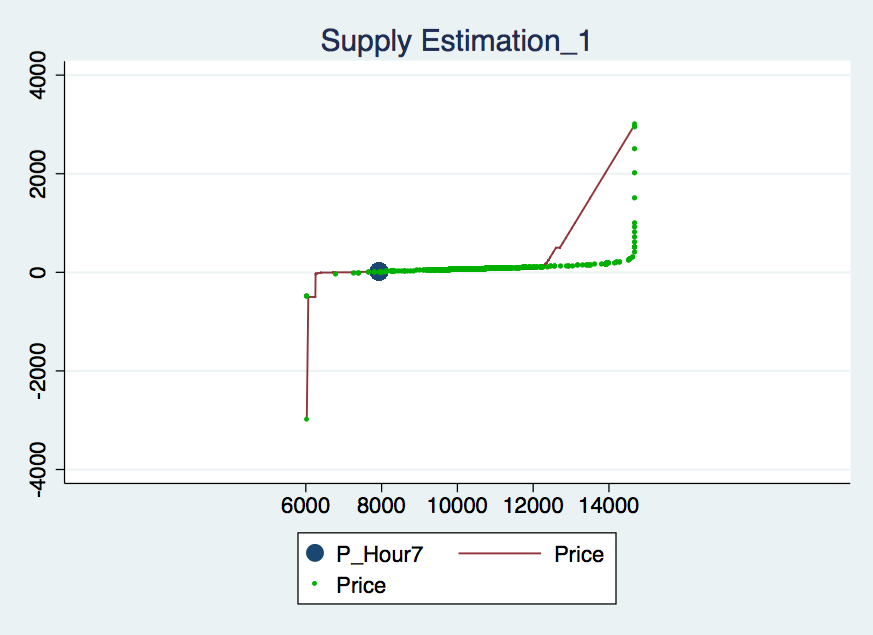
\includegraphics[height=74mm]{figch2/Pic1_C_2011_H7_v30_sym.png} 
} \end{center}
\caption{Example of an assymetric aggregate supply function. The x axis is the quantity in MWh, the y axis if the price in €. In red is the actual aggregate function, in green is an estimated logistic function showcasing the large discrepancies that can arise with this parametric approach. The blue point is the market outcome. }
\label{assymetry}
\end{figure}

The heterogeneity arises from the fact that the bid functions for the electricity auctions are much richer since we have multiple, strategic players on both the demand and the supply side of the market (unlike the market of government bonds, where the supply is monopolistically determined by the Treasury itself). Furthermore, supplier bidding is strongly influenced by the underlying cost of the production technologies. The observed data is consequently less homogeneous and the fitting of the logistic model not convincing. Furthermore, the economic interpretation of the logistic function parameters is very difficult and reducing the whole bid function to two parameters of interest discards a lot of the original information of the bid functions. Finally, we are uncomfortable with the strong assumption of smooth underlying functions and want to circumvent the problems of fitting these.\\

Instead, we develop a non-parametric, functional data analysis approach to select comparable data points from the original bid functions. In our case, this selection of points will yield 4 regions for every curves, each region can be thought of as linear. These selected points are comparable across repetitions of the market (i.e. auctions for different hourly contracts) and can then be used to run a cross-sectional reduced form model. The interest of this approach is threefold. First, it aims to use as much of the original information as possible without distorting it into parameters of a logistic function. What we mean by distortion is the example displayed in Fig. \ref{assymetry}, where one can see that the fitted logistic function in green is very far from the data (in the sense that the integral of the absolute value of the difference of the two curves is very large) because the underlying data simply does not have the proper shape. Also, information about different parts of the bid function does not influence one another, contrary to a parametrized form in which one tries to fit a specified function to data. This implies that the error between the functional form and the data at any point of the curve influences the fitted parameters, therefore ``mixing'' information from the whole curve into the choice of a given value for the parameter. Second, our approach is “scalable” because as many points as necessary can be extracted. The cross-sectional analyses are then conditioned on the type of comparable points selected. Third, while our analysis provides support for an underlying tri-linear or S-shaped functional form, we do not need to assume a specific functional form nor impose overly simplistic assumptions, such as symmetry of the functional forms, to ensure convergence of the estimator.\\

Here we present the methodology of our point selection and apply it to data from the French electricity market. For now, we ignore specificities of the market for the sake of concentrating on the methodology. We introduce very briefly the data and the market in section \ref{gleinfo}. For a full explanation of the data and the market, we refer the reader to chapter 3. In section \ref{pointselect}, we explain the point selection algorithm. In section \ref{pointresults} we discuss the results of the methodology. Section \ref{pointccl} concludes.

\subsection{Information about our data}\label{gleinfo}

Our methodology is general and can be applied to any market where the structure of data observations is similar. Here, we present and discuss the performance of the methodology on data from the electricity market. For the purposes of this chapter we will focus only on the statistical properties of the data, not on the economic interpretation.\\

We apply our methodology to data from a divisible goods auction. In this auction, each buyer and seller submits a full individual bid function, i.e. a demand or a supply function, which consists of 2 to 256 monotone price-quantity combinations. The final bid function consists of these explicitly submitted bid points and all linearly interpolated points between them.\\

The market is cleared by computing the intersection of the aggregate demand and aggregate supply functions, which are each obtained by summing up all individual bid functions for the demand and supply side of the market respectively. In a uniform pricing format, the determined equilibrium price is applied to all units sold in that auction.


\subsection{Point selection algorithm}\label{pointselect}

To briefly fix ideas, let's assume that we are interested in a regression \`{a} la: 
$$ S' = \alpha + \boldsymbol{\beta  X} + \epsilon$$
where $S'$ is the steepness of the bid function, $\boldsymbol{X}$ the stacked vector of exogenous variables (not specified further here), $\alpha$ the regression constant, $\boldsymbol{\beta}$ the stacked vector of regression coefficients and $\epsilon$ the error term. \\

The information $S'$ is drawn from the bid functions of a %the electricity 
market, and varies along the different points of the bids.\\

For comparability, we require that a chosen point $k$ from a supply function must be comparable to the $k^\text{th}$ point from the supply functions of another auction. The same goes for chosen points of the demand functions. The reason for this assumption is that comparing those points accross auction allows us to describe how the functions, that is the aggregate strategies, change shape when our independant variables vary. Note that we do not impose comparability between a pair $k$ of points from a supply and a demand function of the same auction. 

 
\subsubsection{Non-parametric technique to compare bid functions}
\label{comparablepoints}
Consider two demand functions (as shown in figure \ref{comparedfunc}). 
\begin{figure}[!ht]
\centering
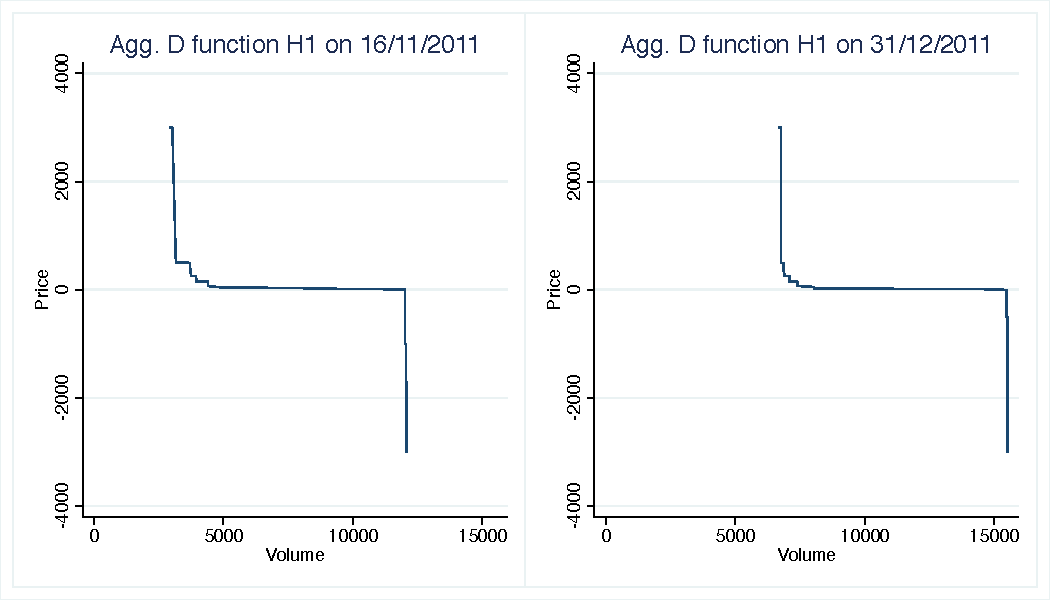
\includegraphics[trim=0.1cm 0.1cm 0.1cm 0.1cm, clip=true, height= 60mm]{figch2/compare2d.pdf}
\caption{Comparison of two aggregate demand functions for the same hour}
\label{comparedfunc}
\end{figure}
 We have to identify "features" of the different functions in order to determine which points can be compared to one another. We aim to reproduce the type of analysis that the brain performs automatically when faced with such curve: we clearly identify three regions of different slope, where the central region is less steep than the left and right regions. \\

To recognise these features, we perform two successive kernel density analyses.\footnote{Bandwidth in the first estimation $=45$, bandwidth in the second estimation $=2$, kernels: epanechnikov.}
For details on the bandwidth and kernel selection as well as algorithm specificities, see appendix \ref{implementingkernel}. This allows us to access estimates of the absolute values of the first and second derivatives of the demand functions as shown in graphs B and C of figure \ref{selectedpoints}.\\ 
\begin{figure}[!ht]
\begin{center}
\makebox[\textwidth][c]{
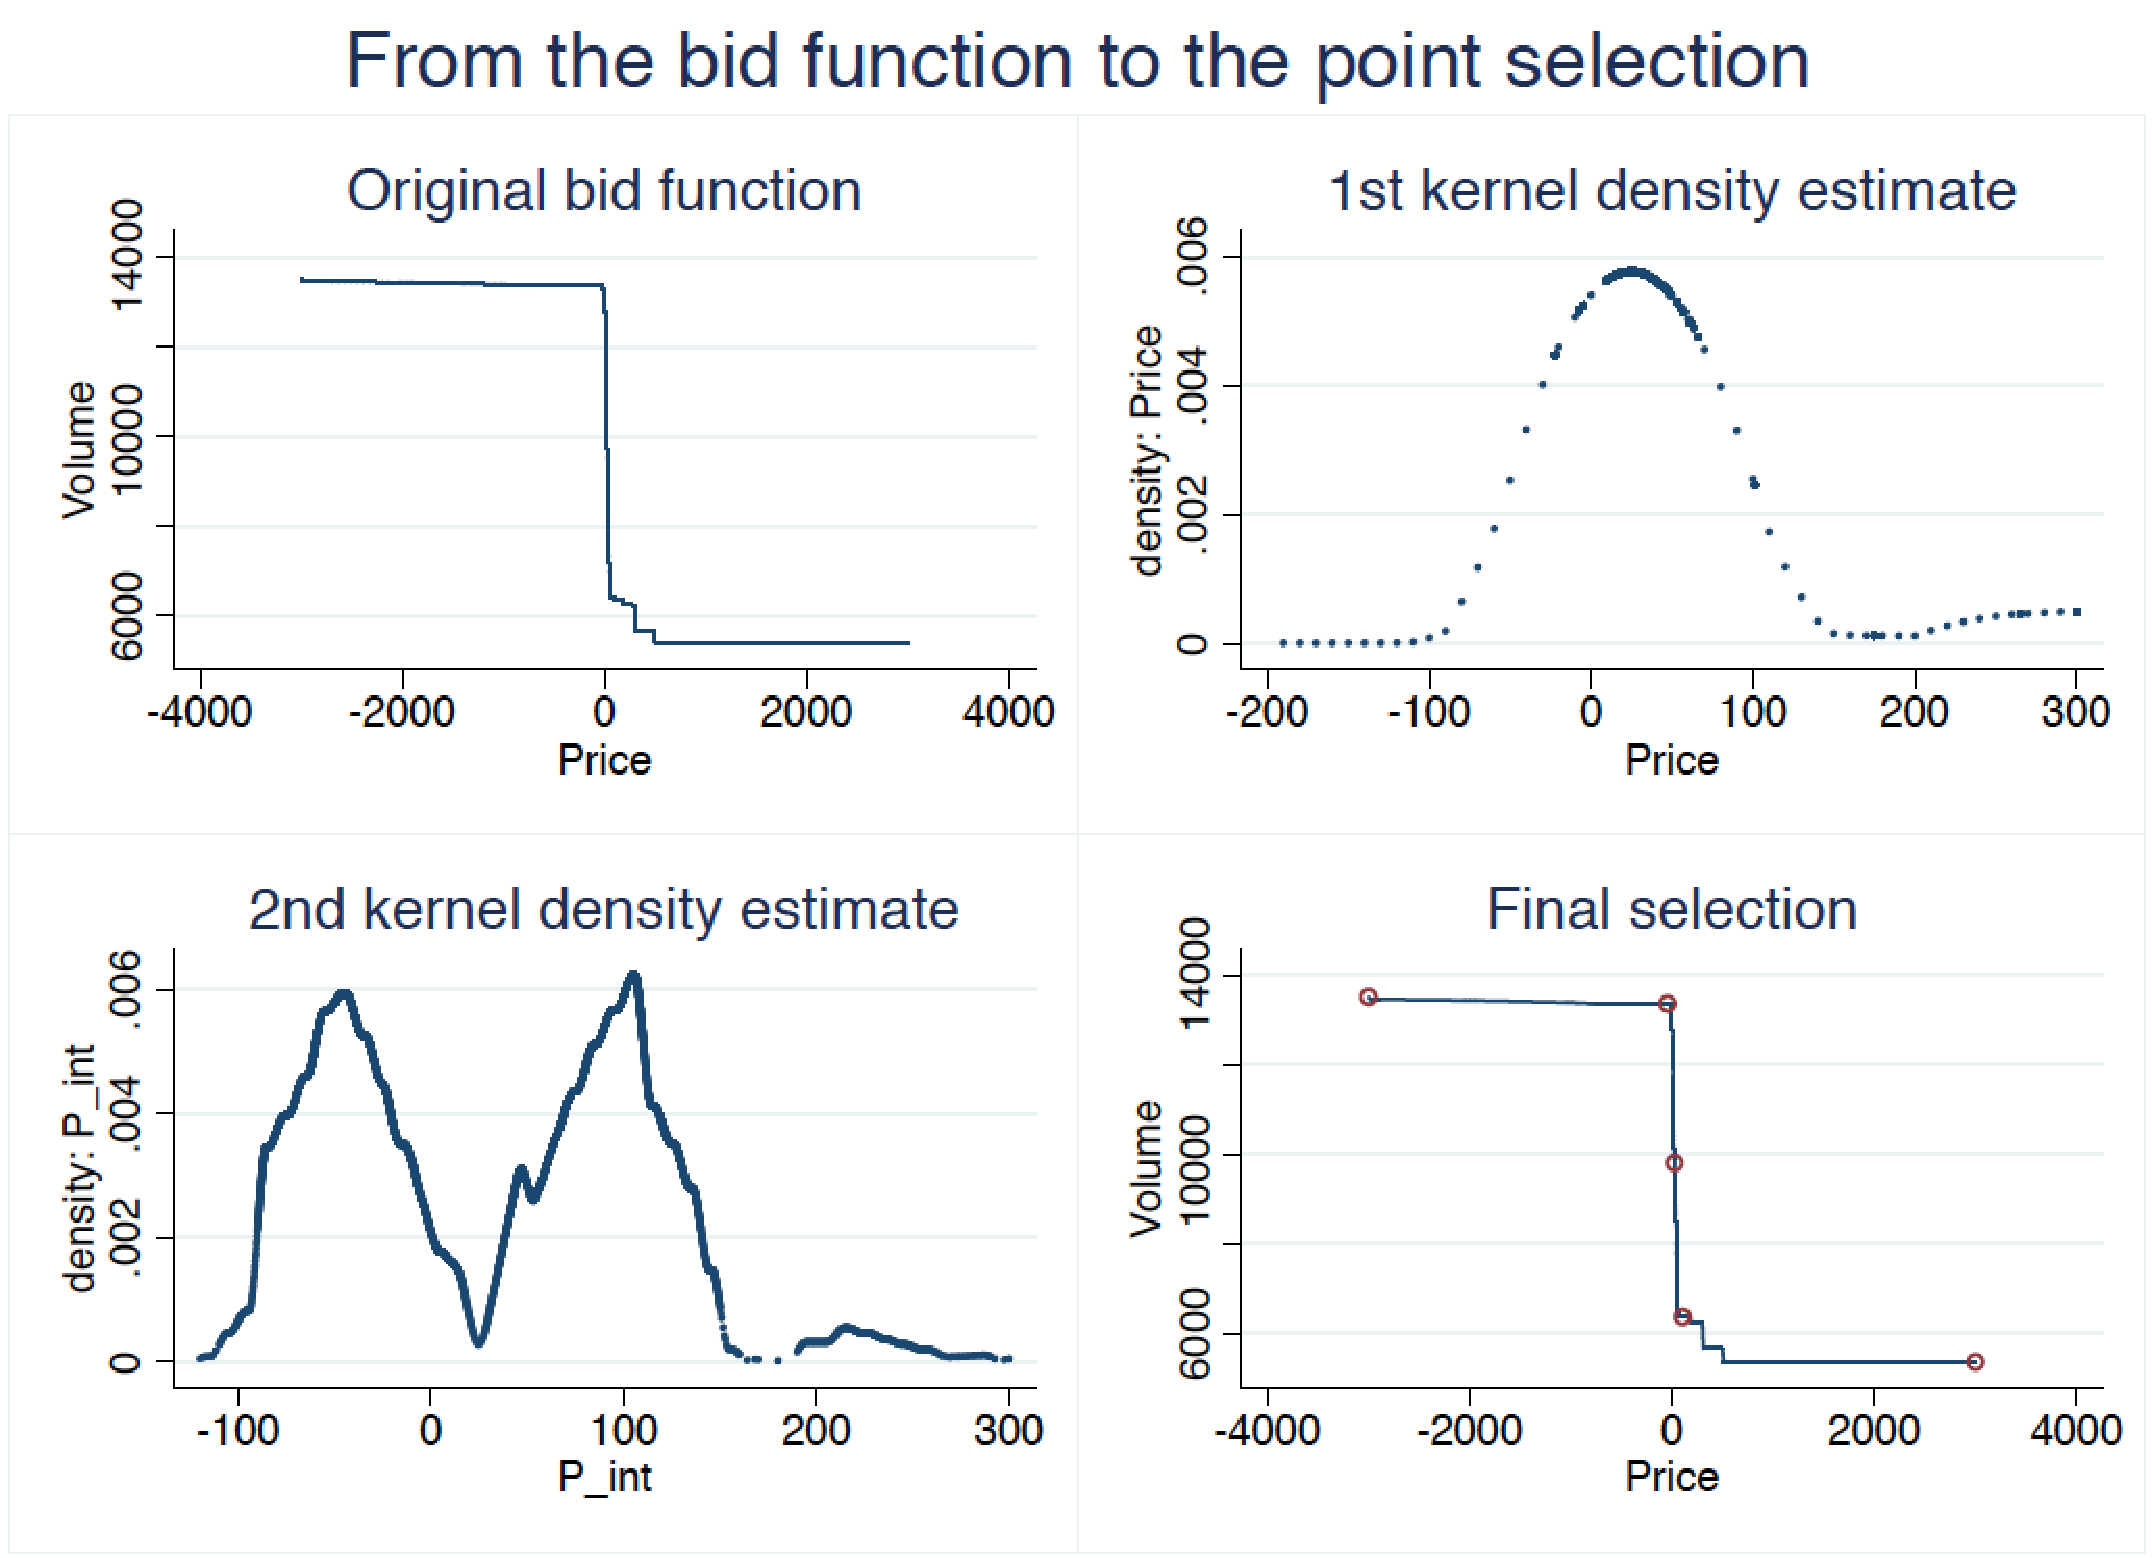
\includegraphics[height= 95mm]{figch2/Shot30.pdf}
}
\caption{Steps of the point selection process}
\label{selectedpoints}
\end{center}
{\small Top left (A): The full original aggregate demand bid function for hour 8 on 15.01.2011 in the quantity - price dimension. Top right (B): Kernel density estimates of the first derivative, zoomed on the relevant price range. Bottom left (C): Zoomed kernel density estimates of the second derivative. Bottom right (D): The full original bid function with the $K=5$ selected points. 
}
\end{figure}

We are therefore able to identify the regions of very high curvature, which define the transition between the three characteristic regions of these functions. We assume that these maxima can be compared across different auctions. This hypothesis is commonly made in functional data analysis and known under the method of landmark registration \cite{ramsaysilverman2005functional}. This has been applied in \cite{wolfi2013interacting}, chapter 4, to day-ahead electricity data, in order to identify the effect of fuel price shocks on supply curves. However, this landmark registration was applied in a parametric form: the regions of high steepness were identified as any part of the curve above 90€/MWh. \\

We can develop this method further and define intermediary points\footnote{As an example, we could extract those points corresponding to half the density value of the maximum density of the second order derivative. The four points selected (one for each monotone portion of the graph of second derivative estimates) would then correspond to those where the curvature of the function is halved. Together with the maximum, the additional point would contain information on the speed (radius of the curvature) at which the function changes.} that can again be compared to one another. This method allows to define as many points as needed, for computational reasons we limit ourselves to $K=5$ points.\footnote{The point selection algorithm took 2 weeks runtime to complete its task of selecting 5 points per function. Defining intermediary points would have taken disproportionately more time since many sorting and interpolation steps are necessary for each intermediate point.} \\

Graph D of figure \ref{selectedpoints} visualises an original demand bid function and the selected points that we retain as an informative summary of the original curve. Once this work is done we are left with $K=5$ points per observed aggregate function, those points being defined in such a way that they can be compared from one auction to another. \\

In our setting, the selected points are the two end-points of the curves (where bidding is imposed by the auction rules at the minimum $(k=1)$ and maximum $(k=5)$ Price), the point corresponding to what can be thought of as the point of inflection (determined by the maximum of the first derivative, $(k=3)$ in the plane $(p,q)$) and the points separating the regions of high and low elasticity in price (determined by the maximum second derivatives to the left $(k=2)$ and right $(k=4)$ of the POI). \\

We described the technique here for the case of a demand function. The information measured at these points can thereby be compared across demand bid functions of different auctions. The method is used analogously for selecting comparable points on the supply function. We are hence able to extract slopes at these selected supply bid points, which are again comparable across auctions.\\


\subsection{Results of the point selection methodology}
\label{pointresults}

\subsubsection{Precision of point selection}
We have selected $K=5$ types of comparable points for each of the $37500$ demand and supply functions present in our dataset. This section details the results of the point selection methodology and presents evidence why the point selection algorithm has produced comparable points reliably. \\

The graphs in figure \ref{g10el} %and \ref{g10hl}
 show the local density of selected points in the price - quantity space for the demand (left) and supply (right) curves.
The fact that the groups of data points are disjoint from one another indicates that the points selected are distinctly different across groups. \\

\begin{figure}[!ht]
\begin{center}
\makebox[\textwidth][c]{
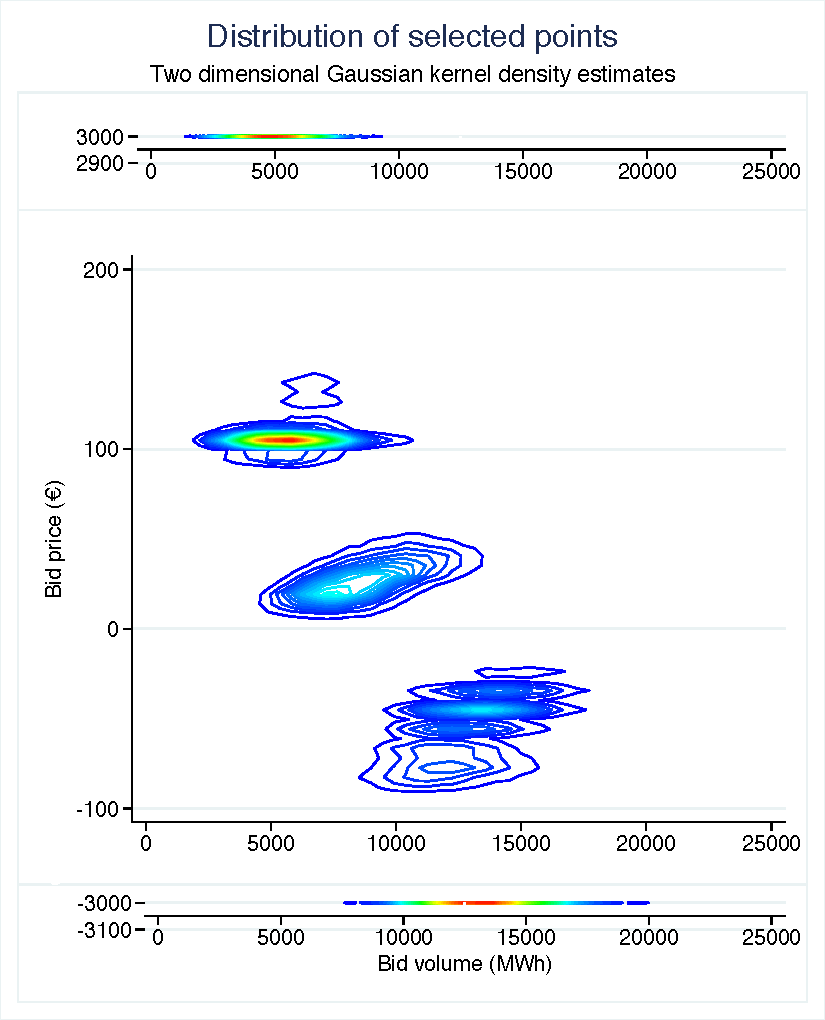
\includegraphics[trim=0cm 0cm 0.4cm 0cm, angle=0, clip=true, height=100mm]{figch2/g10el.pdf}
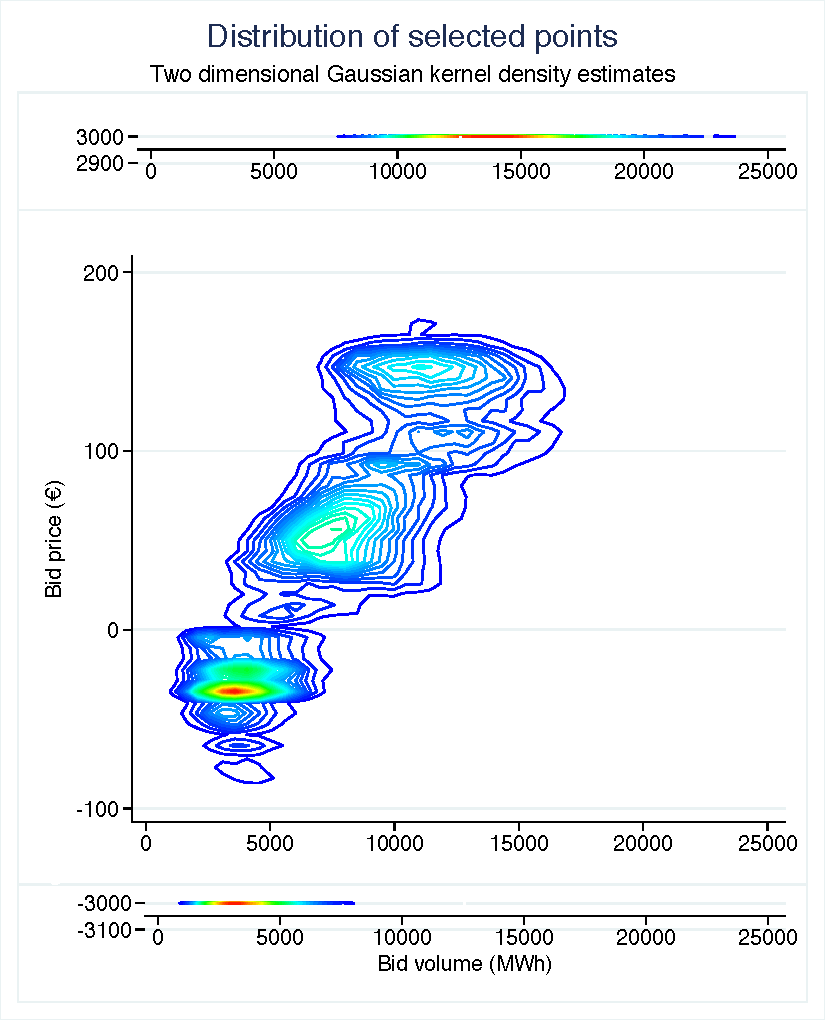
\includegraphics[trim=0.35cm 0cm 0cm 0cm, clip=true, height=100mm]{figch2/g10hl.pdf} 
} 
\caption{Heat map on selected, comparable demand and supply points}
\label{g10el}
\end{center}
{ \small Note: Please note the discontinuity in the scale of the y-axis. The three seperate graphs are arranged to be understood as a single one. The warmer the colours of the heat map, the higher the frequency of selected price-quantity pairs. The colour legend is omitted for brevity, density changes between contours are of the order of $10^{-4}$.} 
\end{figure}


In figure \ref{g10el}, selected points of type $k=1$ manifest at the bottom of the graph with prices fixed at $-3000$\euro /MWh. Similarly, $k=5$ points appear at the top of the graph with prices fixed at $+3000$\euro /MWh. The three distinct groups of data points refer to points of type $k=4$, $k=3$ and $k=2$, respectively, when reading the zoomed, center part of the graph from top to bottom.\\

We note that the point selection for the demand curves has produced groups of points that are more distinct (and thus more robustly attributed to a certain type $k$) then for the supply function. \\

Our methodology only relies on assuming that the first derivative is uni-modal and that sufficient variation exists in the data to distinctly identify the regions of different slope. Overall, this is strong evidence that the algorithm is able to distinctly differentiate between points of different types. \\

\subsection{Observations of bidding frictions}
Distinct point selection is further supported by the evidence in figure \ref{patternsgraph}. These graphs show the distribution in the price-quantity space of the selected points separately for the demand and supply function. Distinct clouds are an indication that selected points are different across types $k$.\\

\begin{figure}[!ht]
%\begin{center}
\makebox[\textwidth][c]{
%\includegraphics[height=65mm]{g10b2.pdf} 
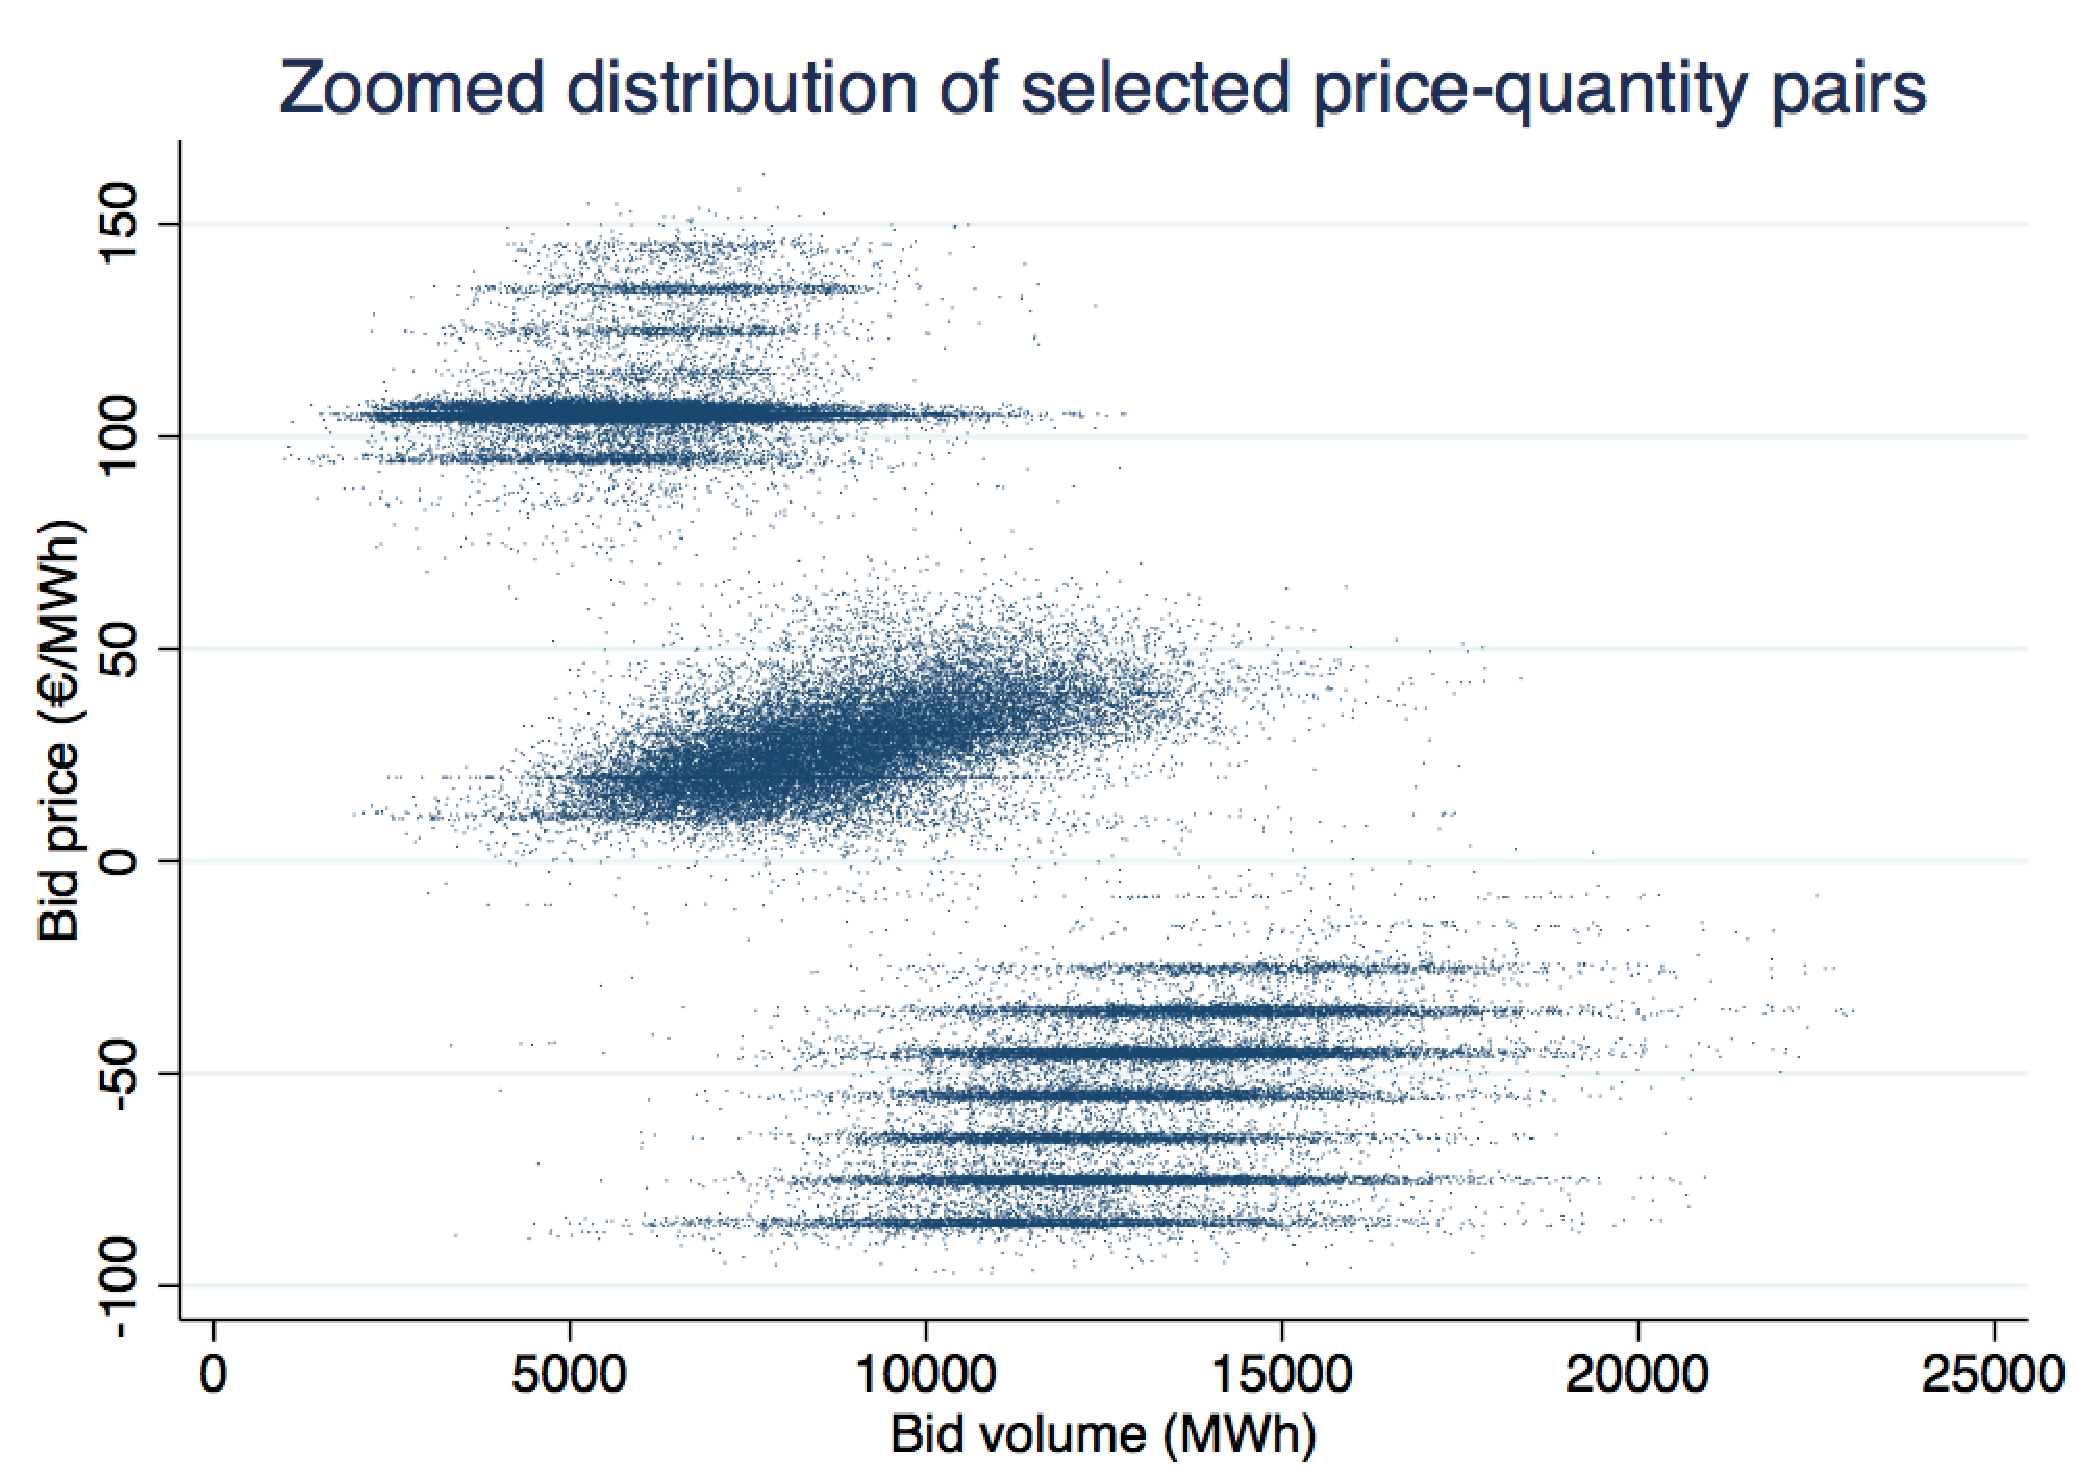
\includegraphics[trim=0cm 0cm 0cm 2.5cm, clip=true, height=48mm]{figch2/Shot06.pdf} 
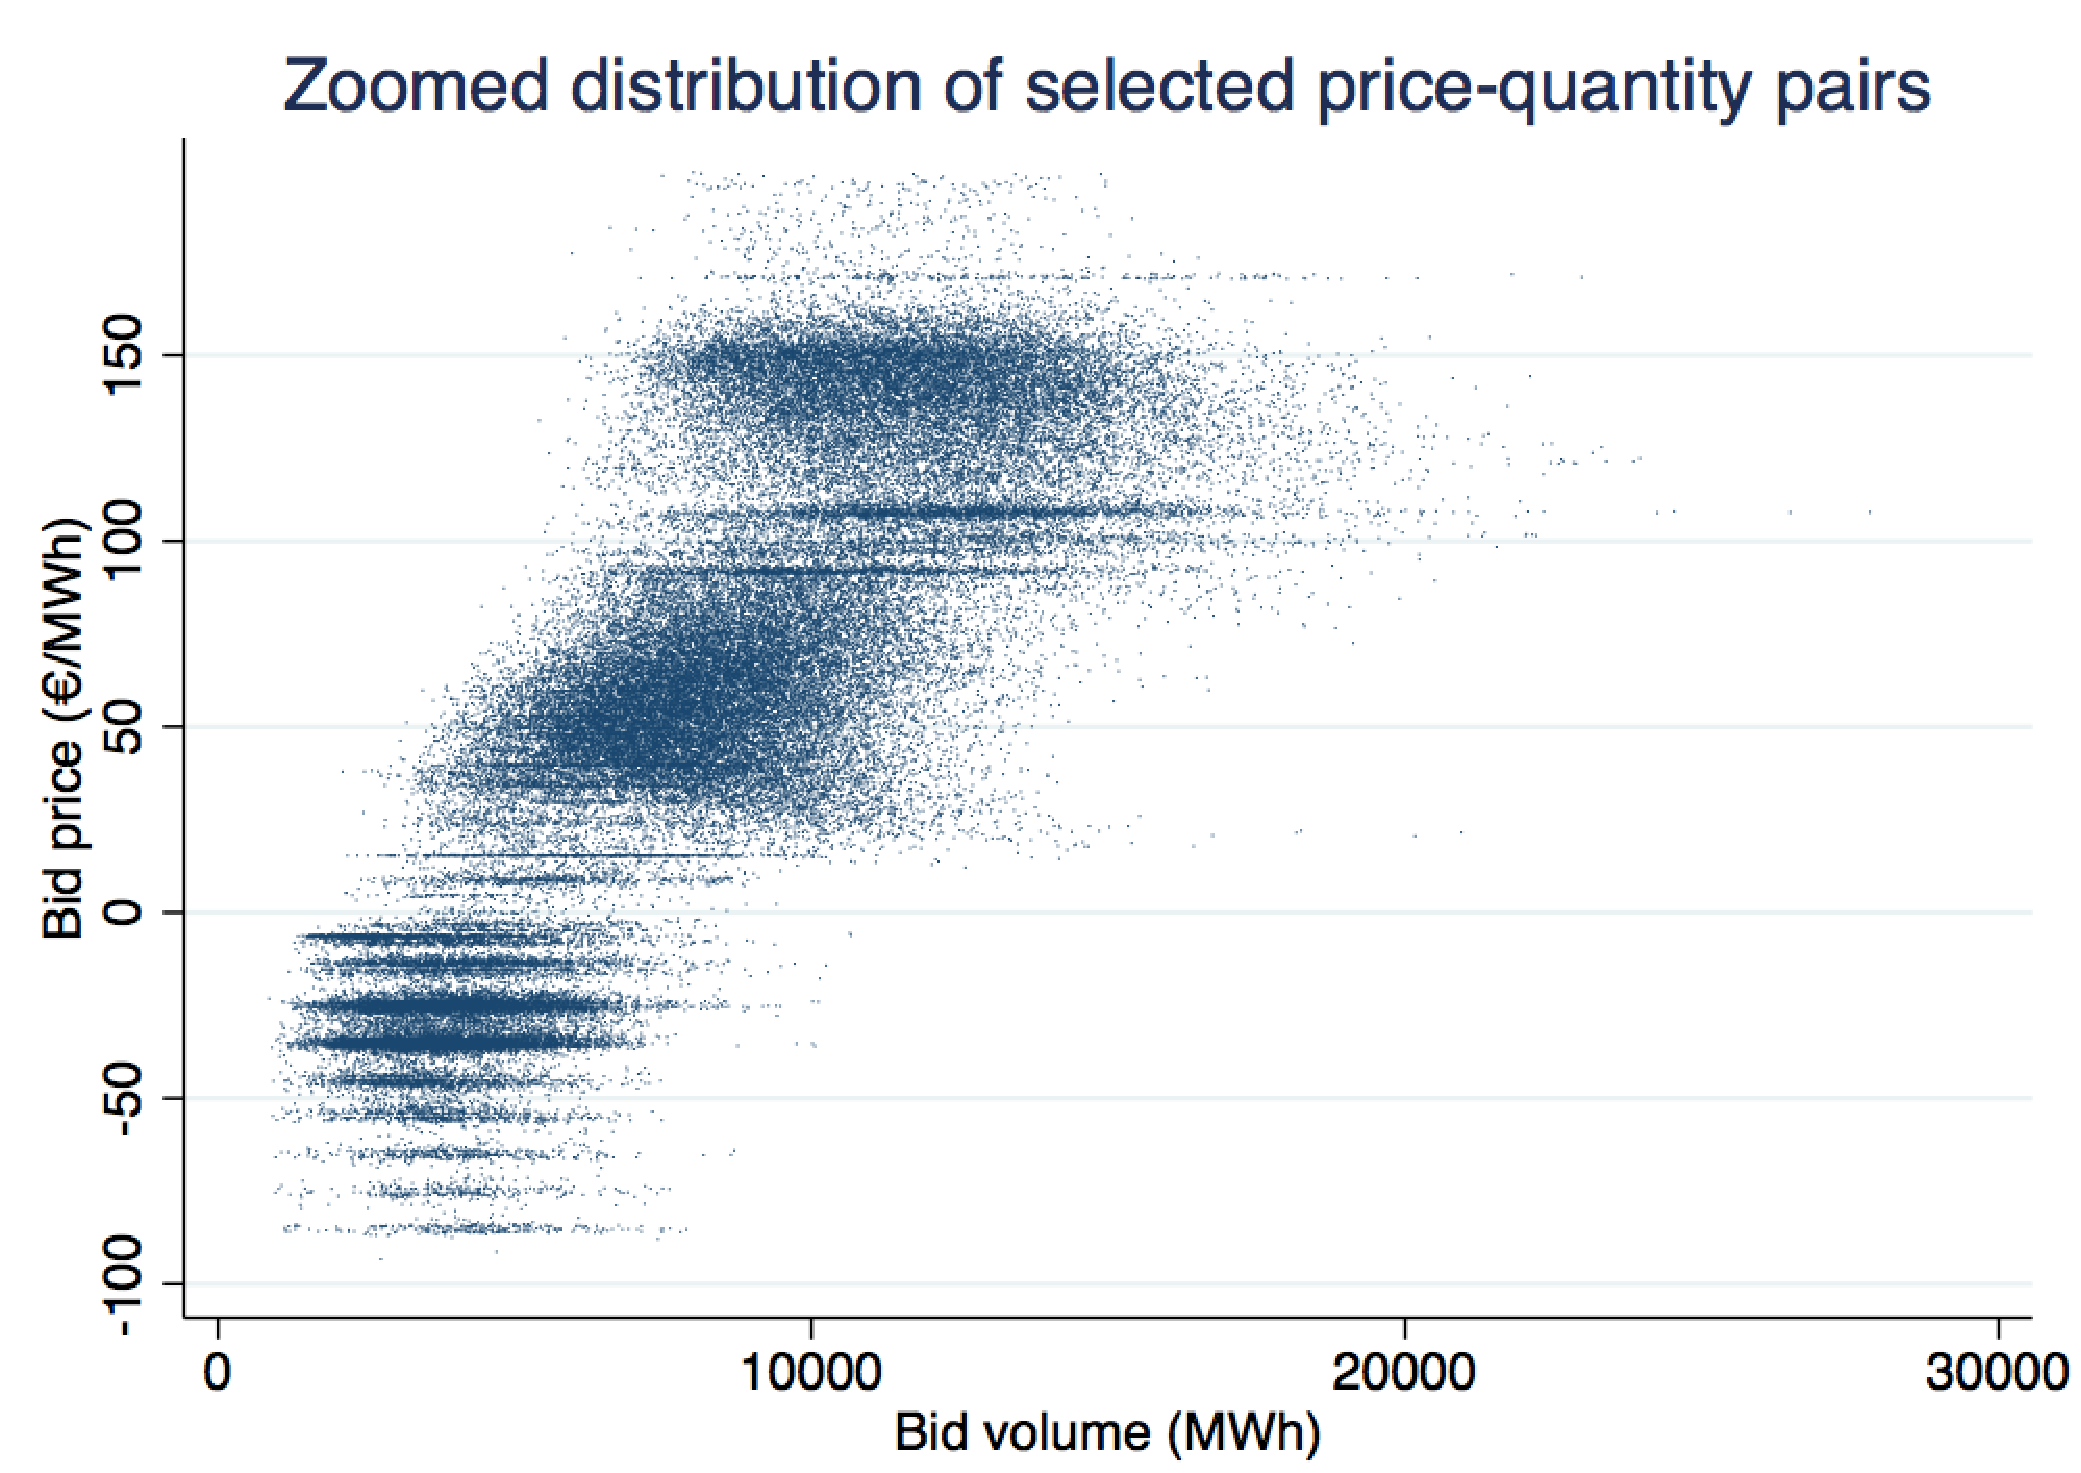
\includegraphics[trim=0cm 0cm 0cm 2.5cm, clip=true, height=48mm]{figch2/Shot15.pdf} 
}
\caption{Distribution of selected demand (left) and supply (right) points}
\label{patternsgraph}
%\end{center}
%{ \small Note: This graphs shows the zoomed distribution of the selected points in comparison to the heat map in figure \ref{g10el}.} 
\end{figure}


However, a feature of the graphs is striking: patterns (horizontal lines) seem to exist for the selected points of type\footnote{Types $k=1$ and $k=5$ do not exhibit variation in price, because bidding at the extreme prices of  +-3000\euro{}/MWh is imposed by the auction rules. We thus neglect their analysis here.} $k=2$ and $k=4$. Many selected points accumulate at certain prices of regular intervals of 10\euro{}/MWh, i.e. there seem to be focal price points for the bidders at the curvature points of the bid functions. The pattern is present for selected points of both the supply and demand functions, although the selected points from the supply function exhibit this pattern slightly less. \\

The points following the pattern (types $k=2,4$) represent the points of maximum curvature of the aggregate bid functions, i.e. the region where the aggregate bid function transitions from a price elastic center portion to the price inelastic extremities of the bid function. \\

%While we do no have a story for this phenomenon, 
Without prioritizing any explanation\footnote{We do not investigate the origins of bidding frictions in this section, we focus purely on  the methodology. For the electricity market, a few possible explanations are that (1) bid functions are driven by marginal costs consideration towards the extremes of the bid curve, (2) bidders bid coarsely since they have used up much of their bid point allowance (256 points) on the center portion of the curve, (3) bidders spend less effort on adequately bidding at extremes since the likelihood of the market outcome occurring at the extremes is much lower. }, we acknowledge the existence of bid point patterns in the values (i.e. prices and quantities) of selected points. \\

We are, however, interested in $S'$, the slope at each selected point - an information measured at the selected point. We therefore investigate whether the values of the first derivative at the selected points display a pattern. Figure \ref{histpattern1} shows the histograms of slopes of supply functions for the points $k=2,3$ and 4. No pattern in the values of the derivatives is apparent. \\

\begin{figure}[!ht]
\begin{center}
\makebox[\textwidth][c]{
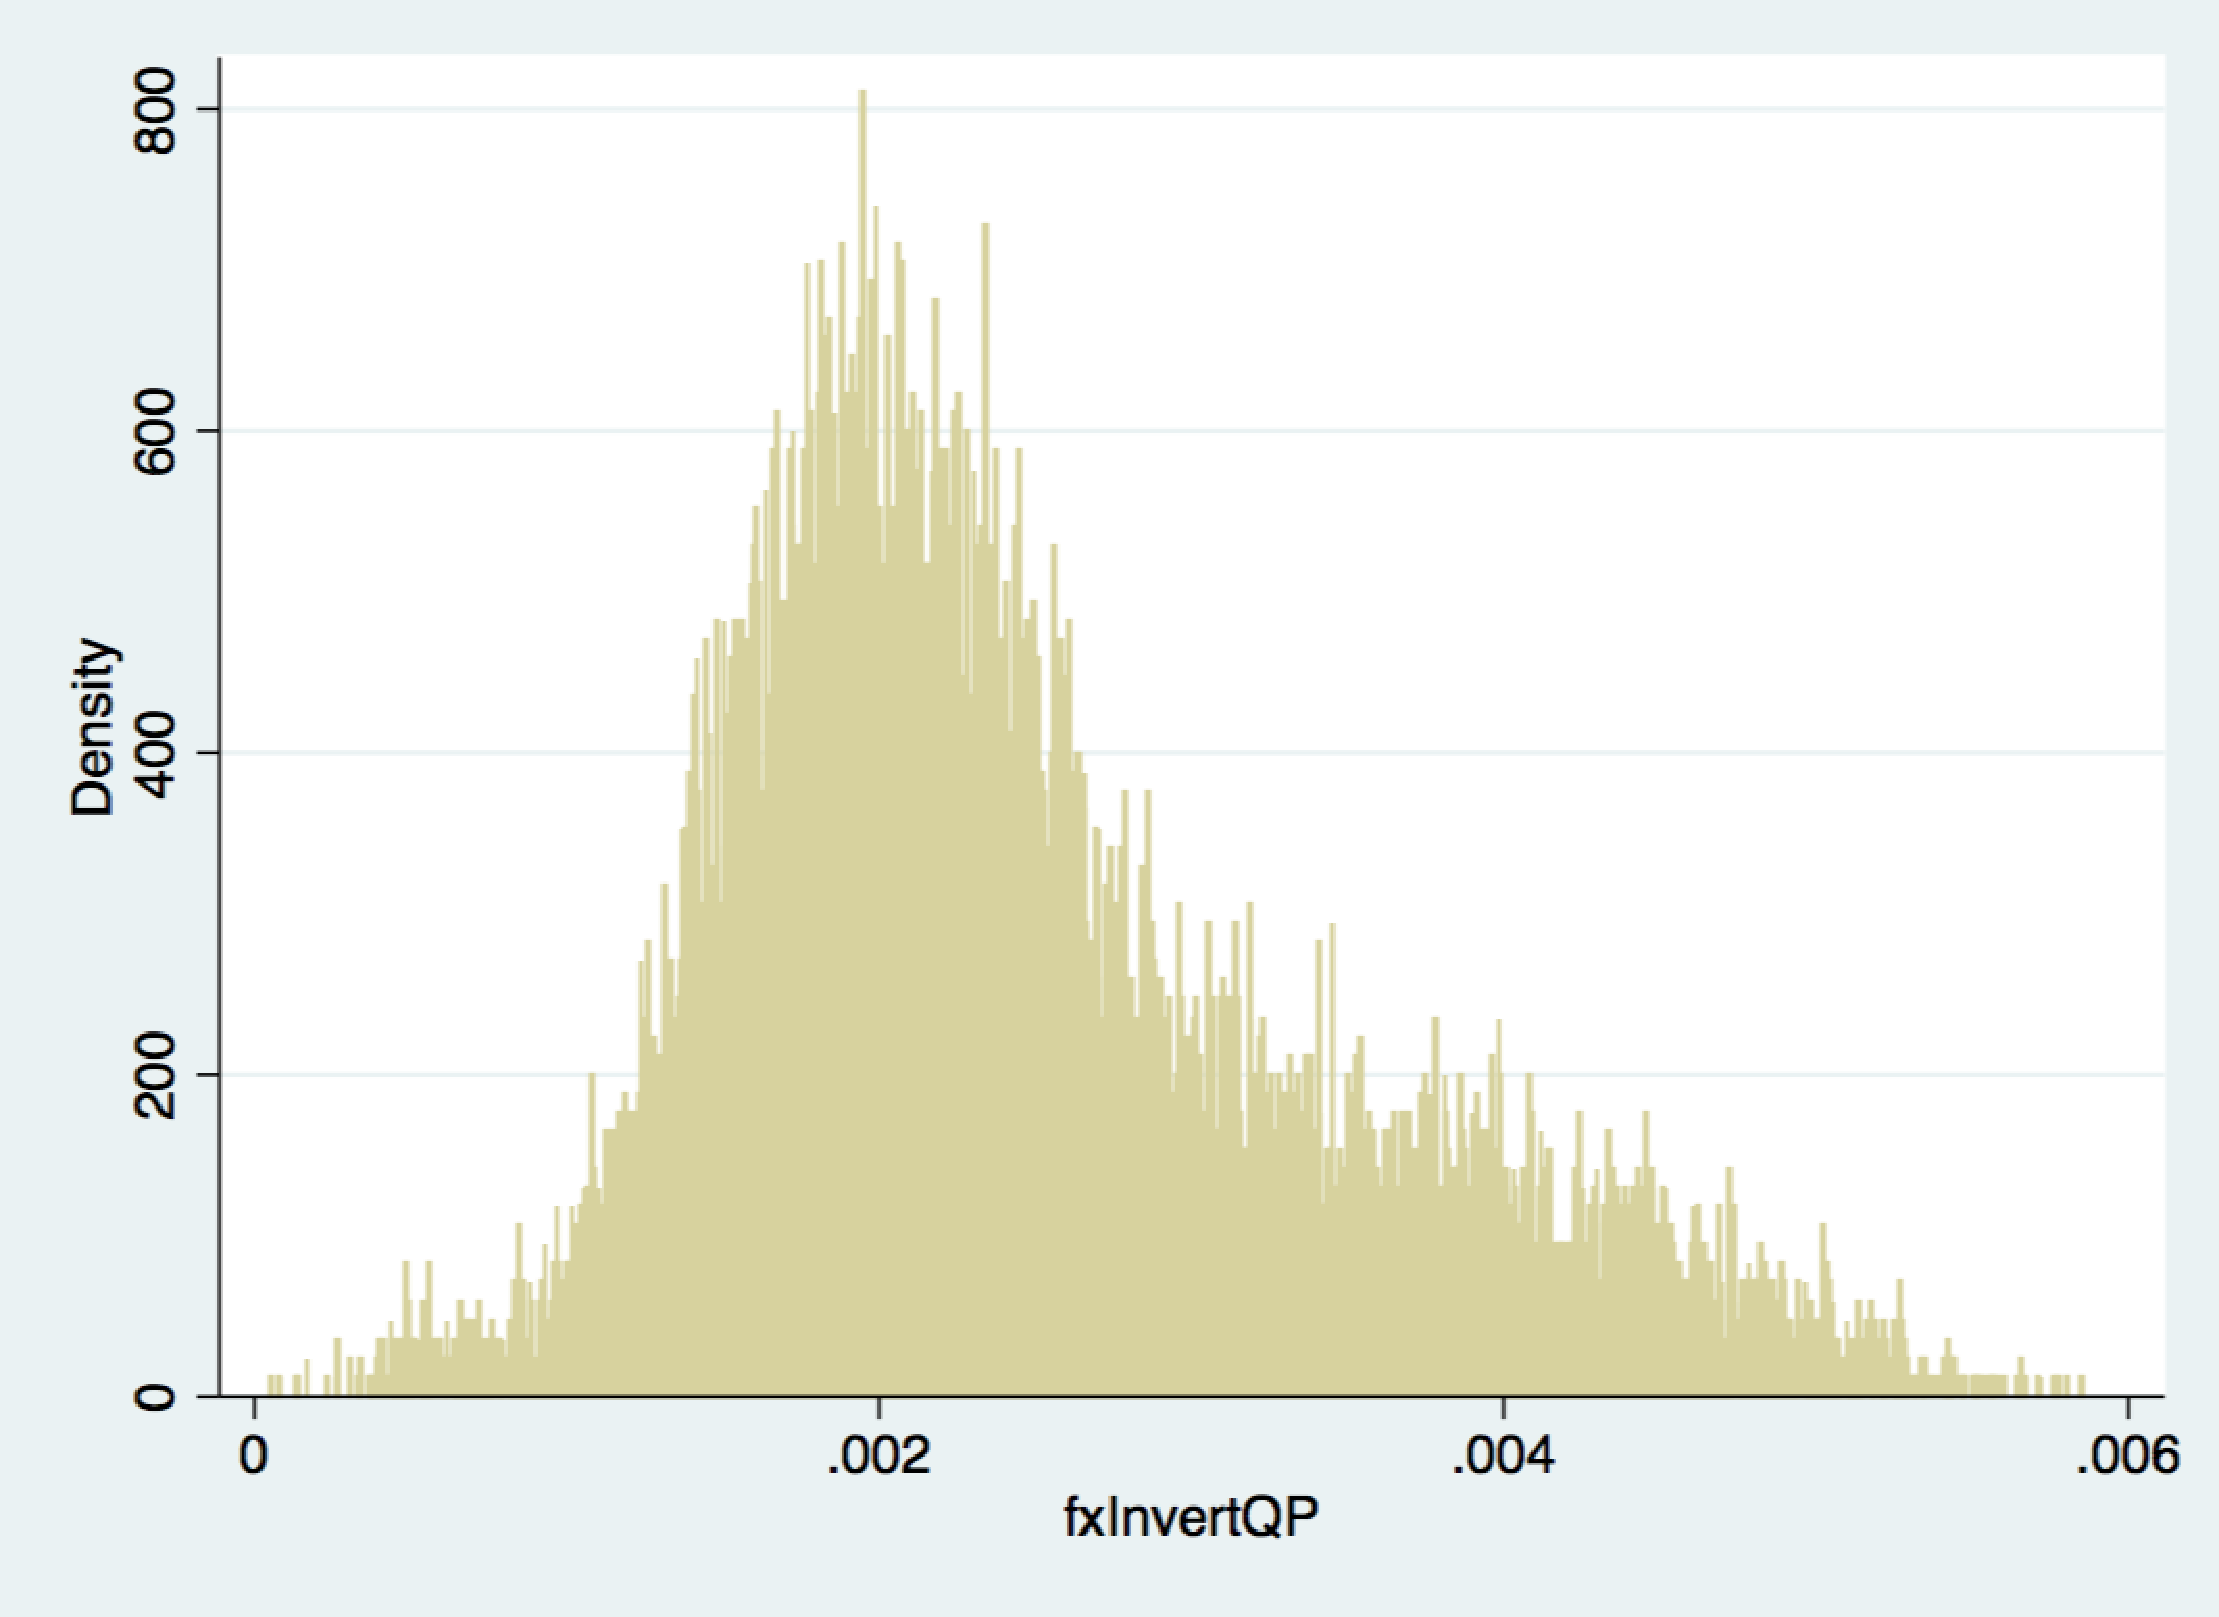
\includegraphics[trim=0cm 0cm 0cm 0cm, clip=true, height=35mm]{figch2/histslope3.pdf} 
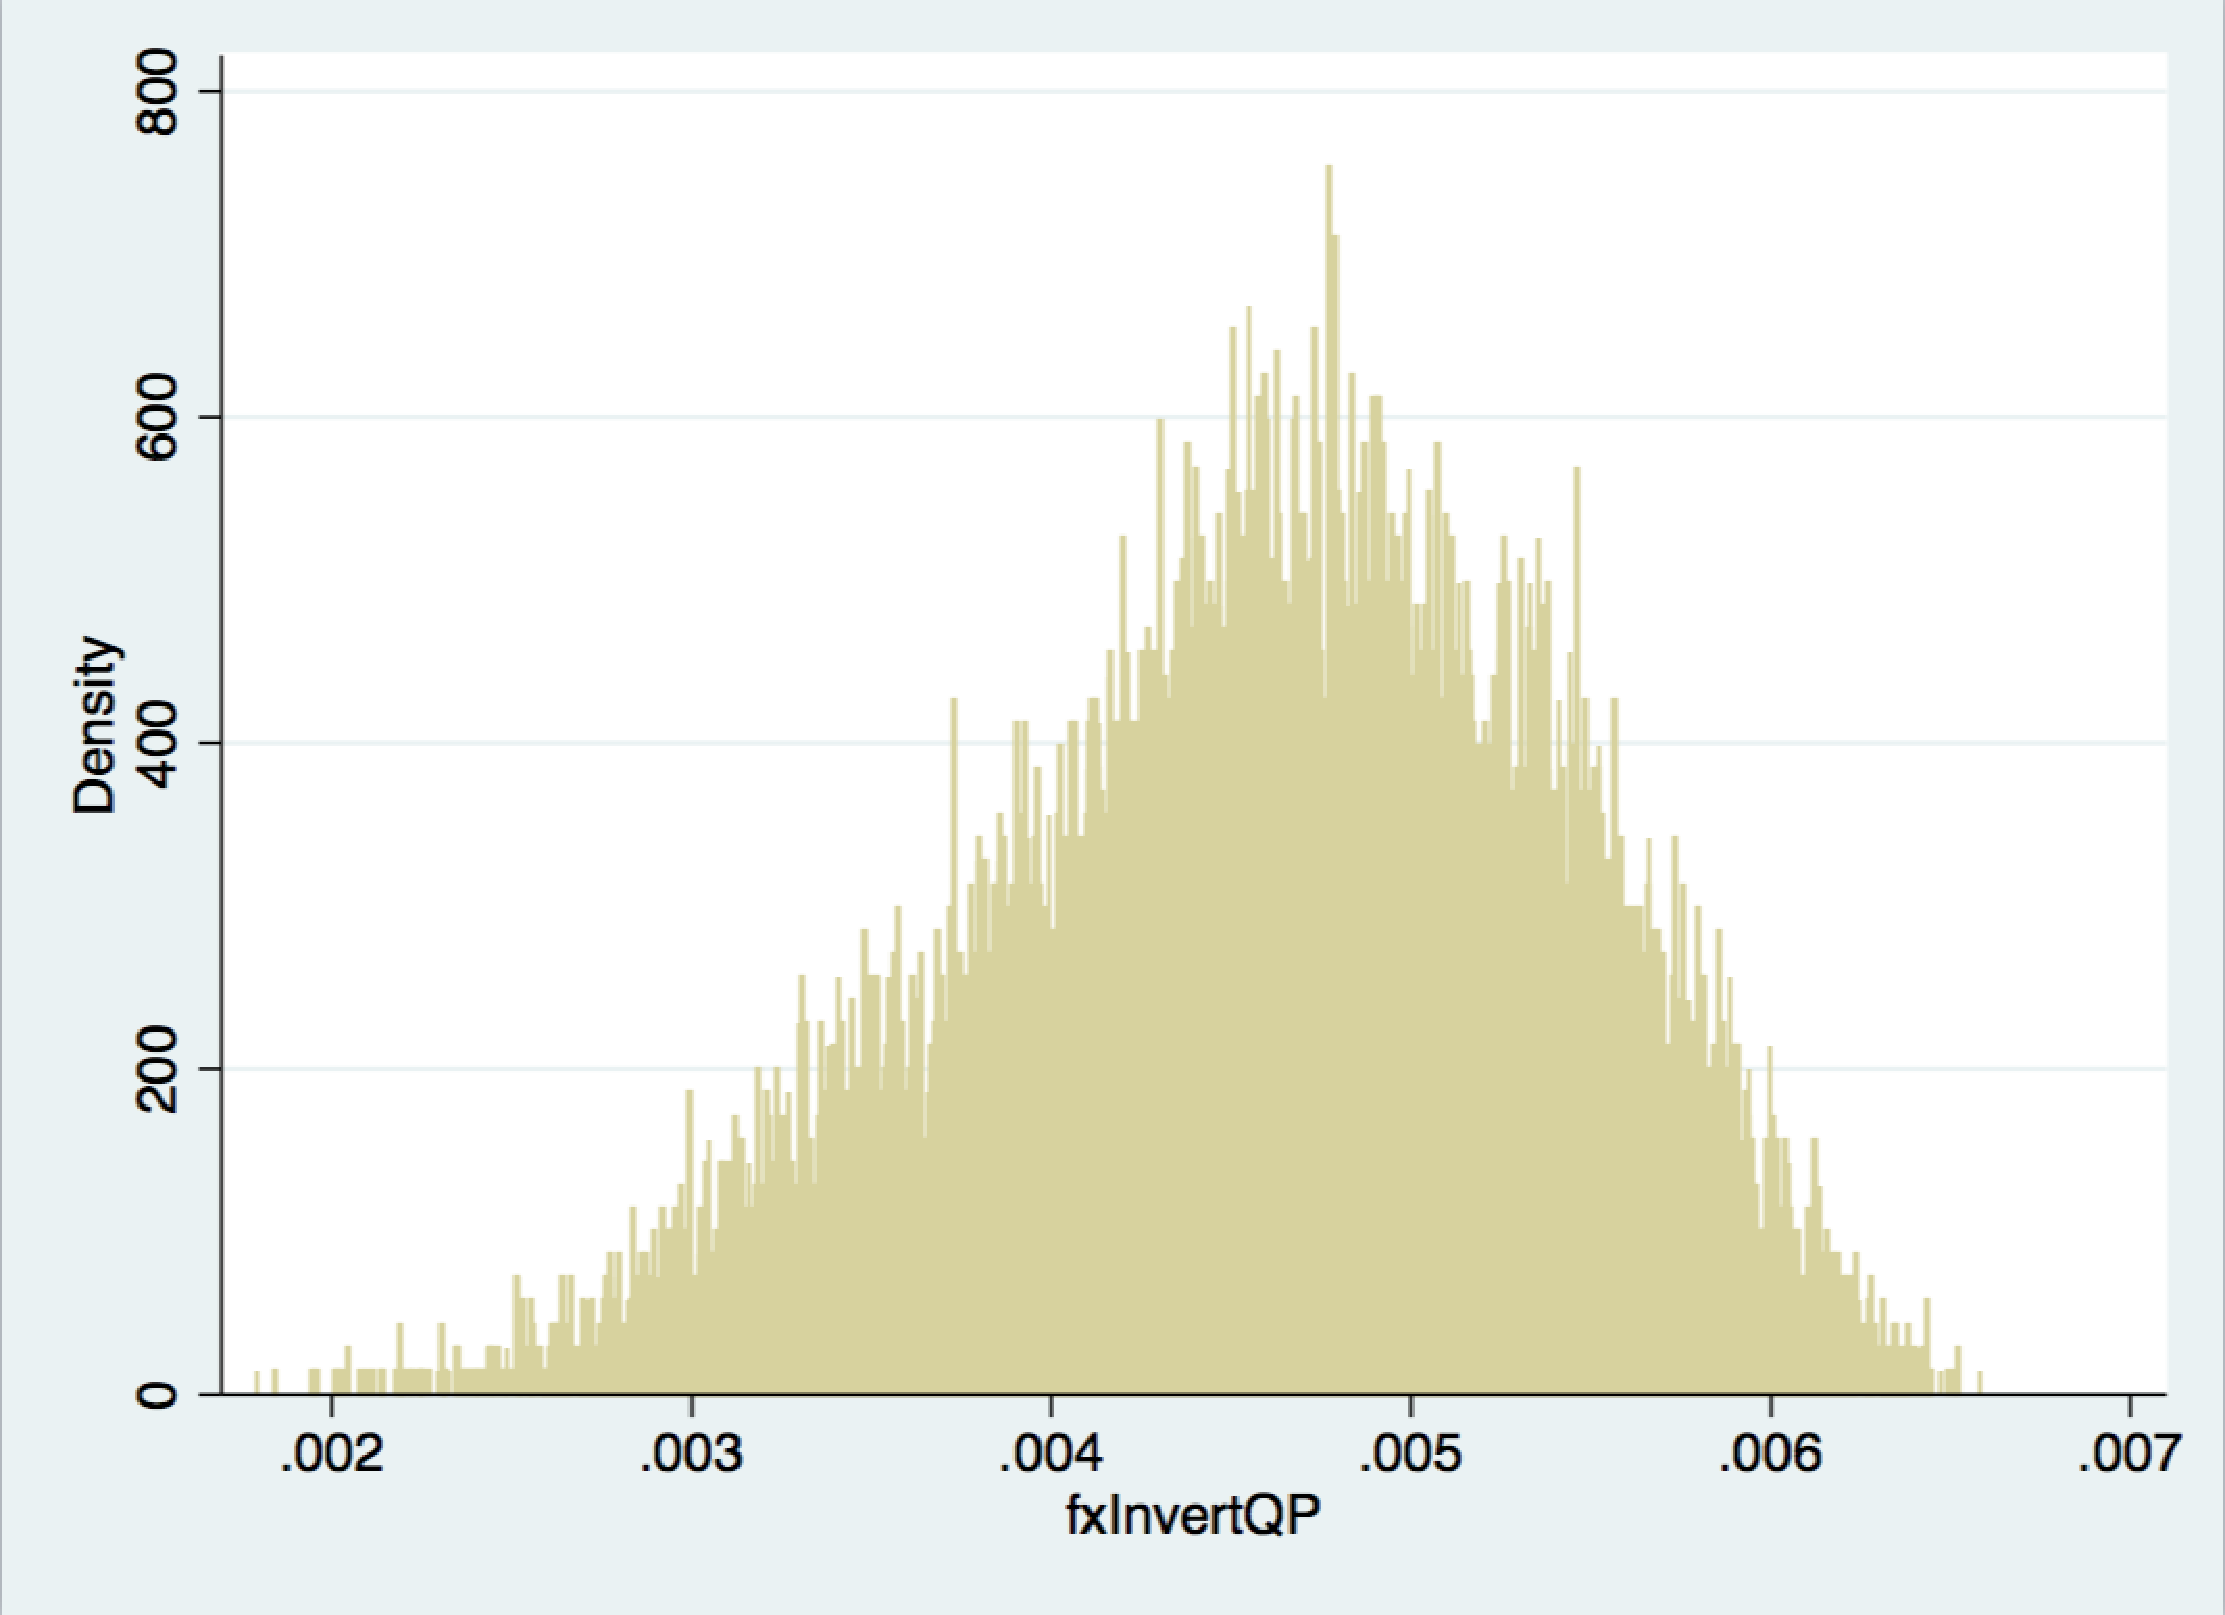
\includegraphics[trim=0cm 0cm 0cm 0cm, clip=true, height=35mm]{figch2/histslope5.pdf} 
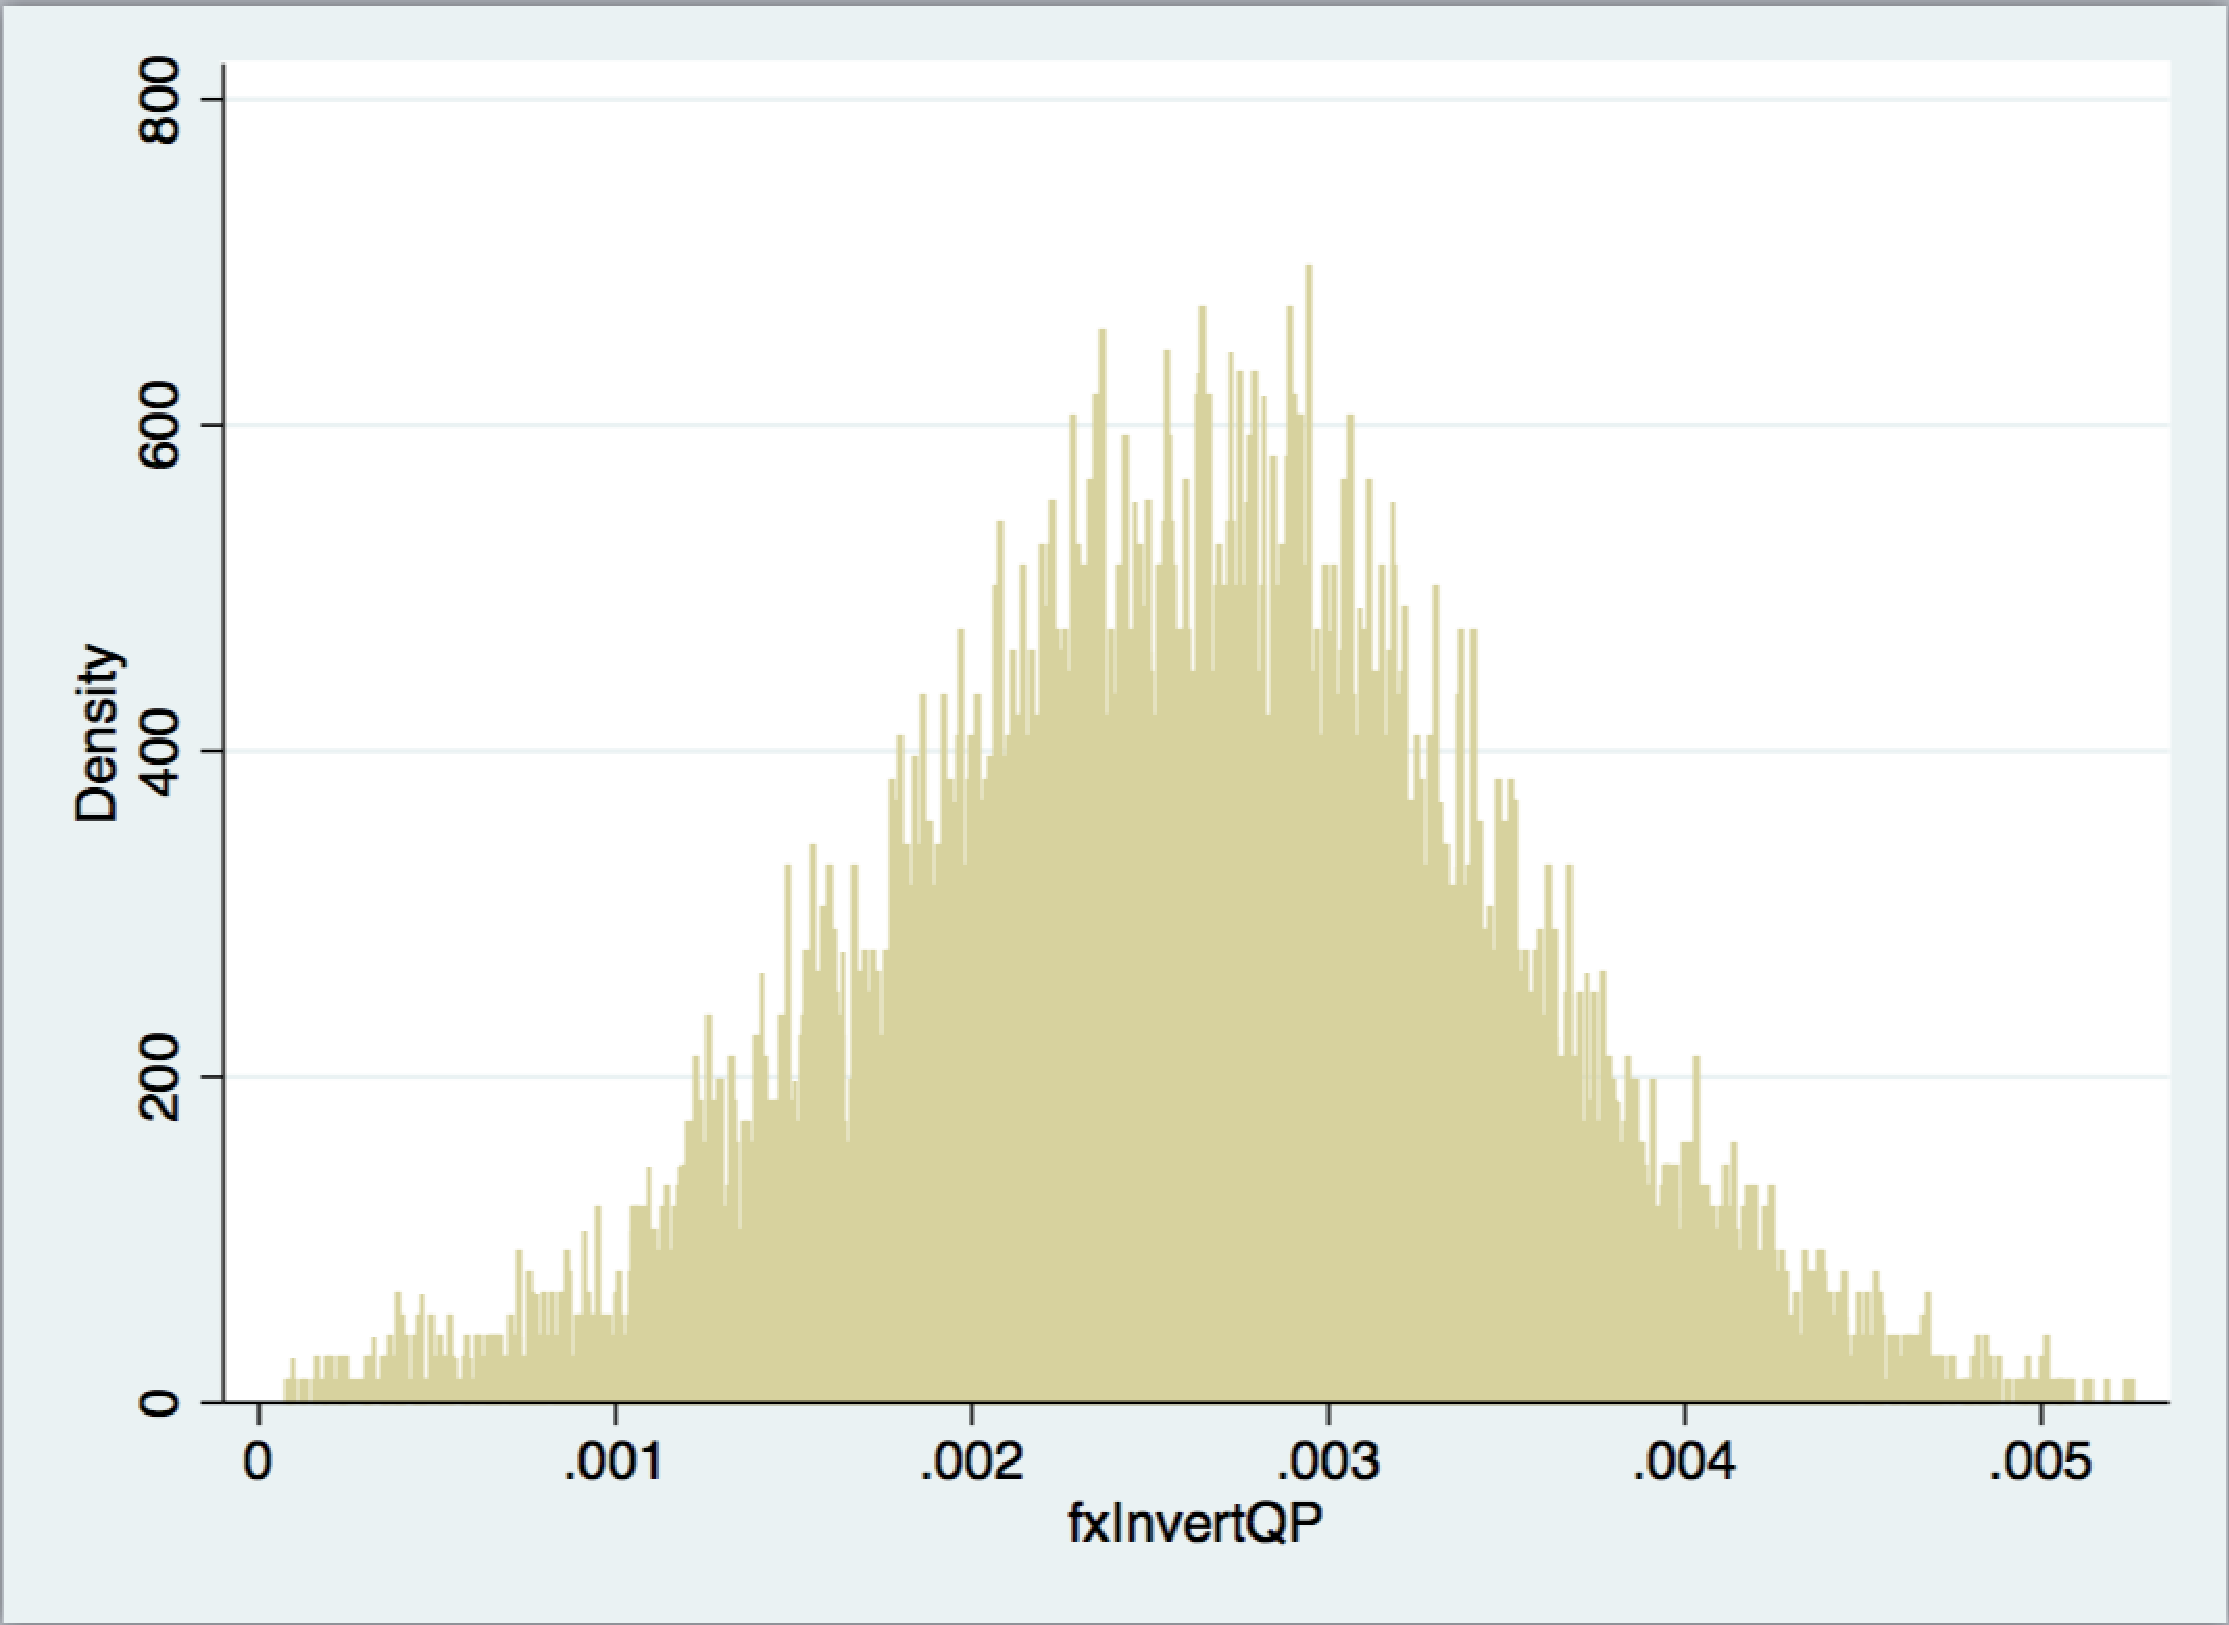
\includegraphics[trim=0cm 0cm 0cm 0.1cm, clip=true, height=35mm]{figch2/histslope7.pdf} 
}
\caption{Histogram of slopes per point type}
\label{histpattern1}
\end{center}
{ \small Note: Histograms of extracted slopes at points of type $k=2$ (left), $k=3$ (middle) and $k=4$ (right).} 
\end{figure}
% STATA COMMAND: hist fxInvertQP if select==7, bin(1000)


Although values of the selected points are possibly biased due to focal price points, we do not observe patterns in the variable of interest (i.e. the first derivatives of the selected points) and deem the methodology adequate for our purposes. \\

Finally, we emphasize that the observed patterns are not caused by the point selection mechanism since the algorithm can only choose between explicitly bid points or linearly interpolated points, that could be part of a market equilibrium under the reigning price setting algorithm. The pattern arises from many horizontal steps occurring at the same prices in different auctions. 


\subsubsection{Value of selected points (determining $K$)
%Degrees of freedom of the inferred bid function
}
We remind the reader that the aim is to recover points that summarize well the behaviour of the full aggregate bid functions in different auctions. 
Our technique allows us to extract representative and comparable points across bid functions of different auctions. Form the selected points, we can also go back to infer the original bid function from which the points were selected. In order to evaluate the utility of our methodology, we investigate the added benefit of an additional point in our point selection. \\

By selecting $K=5$ points per curve, rather than fewer points per curve, we are able to significantly reduce the degrees of freedom for inferring the original bid function. In other words, our information (as captured by the selected points) about the original bid function is more precise. \\

In order to investigate the marginal gain of information for additional points, we first define the mean registered curve. Consider a set of curves that each have N registered points. Take the average coordinates of every point across curves. Rescale linearly every curve by parts so that the registered points fall on their average.\footnote{We rescale all points between the reference points by a vector obtained as a linear combination of the displacement vectors of the closest reference points, of which weights are obtained as the inverse of the distance of the considered point to the enclosing reference points.} Define the mean registered curve as the averaged rescaled curves. Now, separate the data into two groups: curves that are above or below this average curve. Take the averages of these two groups: this defines a measure of the variability of the curves around the total average which is able to capture asymmetries between the two groups.\\

Now that these quantities are defined, we can display how much information is captured by the successive addition of registration points for $K=0$ to $K=5$ points. We look at the decrease in uncertainty achieved by including an additional point, obtained using our technique. Figure \ref{errorbarsasfunction} shows the mean registered curves (red lines) and the mean inferior or superior curves (pink shaded interval above and below the mean registered curves) as a function of the number of reference points. \\

\begin{figure}[!ht]
\begin{center}
\makebox[\textwidth][c]{
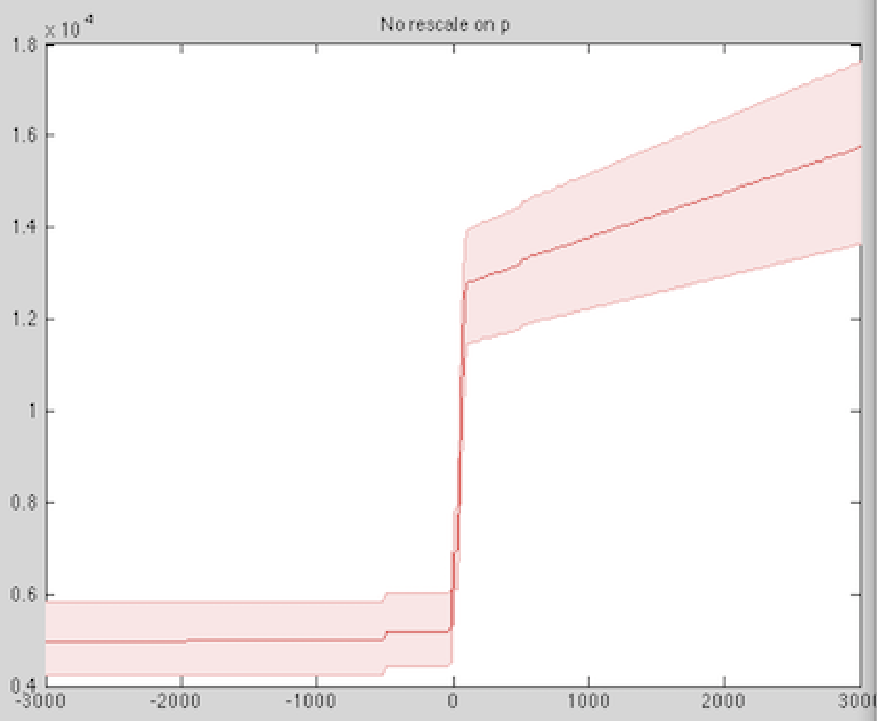
\includegraphics[trim=0cm 0cm 0cm 0cm, clip=true, height=50mm]{figch2/MC3.pdf} 
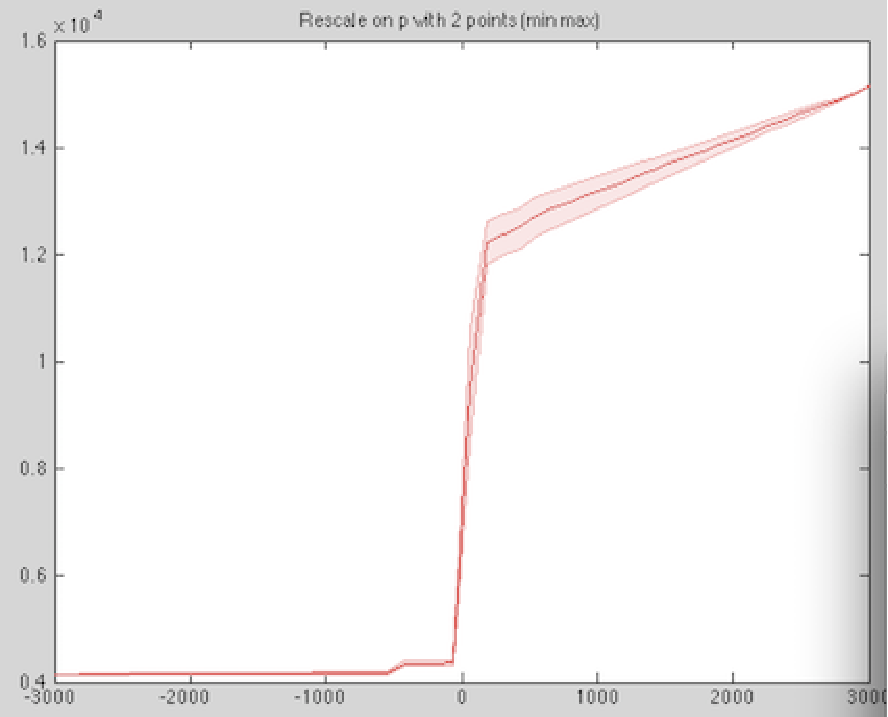
\includegraphics[trim=0cm 0cm 0cm 0cm, clip=true, height=50mm]{figch2/MC4.pdf} 
} \\
\makebox[\textwidth][c]{
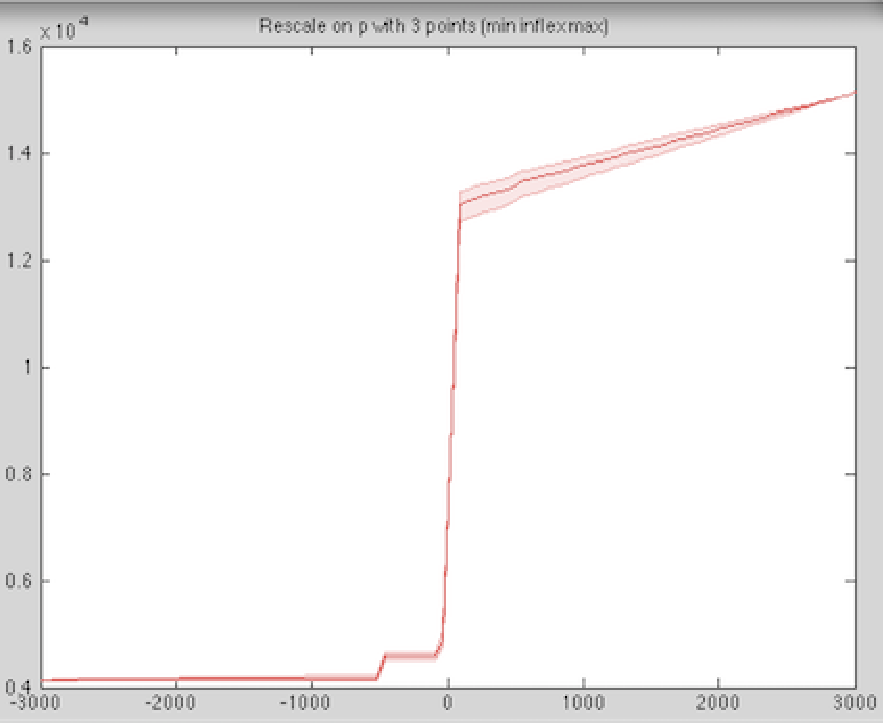
\includegraphics[trim=0cm 0cm 0cm 0.1cm, clip=true, height=50mm]{figch2/MC5.pdf} 
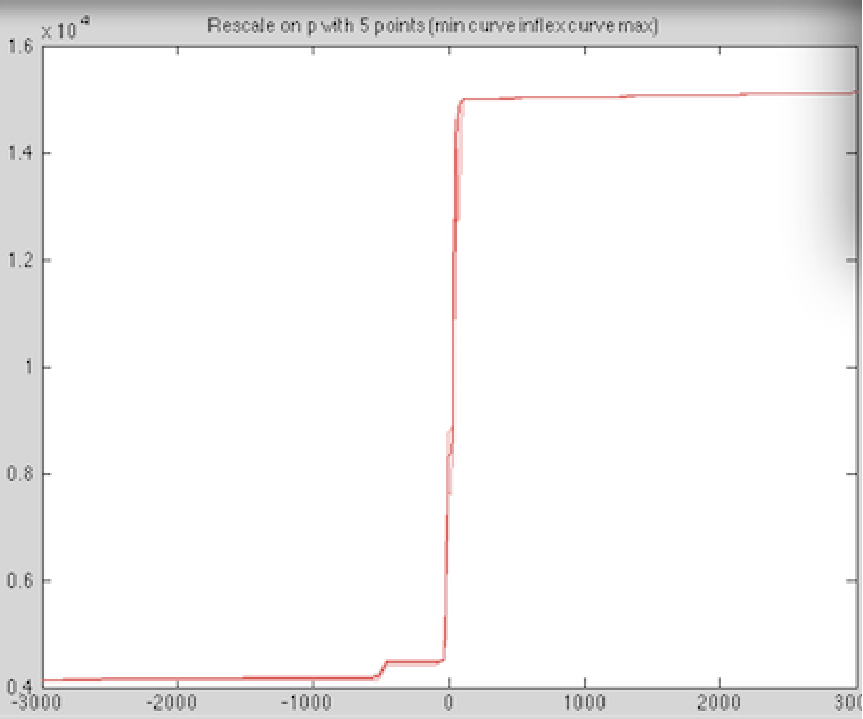
\includegraphics[trim=0cm 0cm 0cm 0.1cm, clip=true, height=50mm]{figch2/MC6.pdf} 
}
\caption{Error bars as a function of the number of extracted points}
\label{errorbarsasfunction}
\end{center}
{ \small Note: The graphs represent the master curve with the error interval for inferring the original bid function, conditional on the number of extracted, reference  points (RP). Top left (A): Computed without any RP. Top right (B): Computed using 2 RP. Bottom left (C): Computed using 3 RP. Bottom right (D): Computed using 5 RP. } 
\end{figure}

We can see that as we include an increasing number of points the shaded areas shrink: this is a measure of how much of the information contained in the raw curves is captured by the registration points. We see that at 5 registration points, the shaded area is very small, so much so that one can consider that by registering these 5 points, we capture a so-called "master curve": most of the information about the curves is contained in those 5 points.\\

More quantitatively: without any reference point, inferred bid functions would lie in the interval shown in graph A of figure \ref{errorbarsasfunction}. With two reference points (namely the minimum an the maximum quantity), the uncertainty is reduced as shown by the smaller error interval in graph B. Graph C adds a third point (the inflection point) and Graph D adds another two points (the two points of maximum curvatures). Figure \ref{errorbarsasfunction} shows clearly that with an increasing number of reference points, we obtain a more precise information about the original bid function. We quantify the informational gain by measuring the pink shaded area in each graph A to D. The result is shown in figure \ref{decreasingdegreesoff} and reveals decreasing marginal information for each additional point. By selecting $K=5$ points, we are able to reduce the shaded area by a factor of about 50 when compared to figure A (see figure \ref{decreasingdegreesoff}). We see this insight as support for using $K=5$ points for further work. \\

\begin{figure}[!ht]
\begin{center}
\makebox[\textwidth][c]{
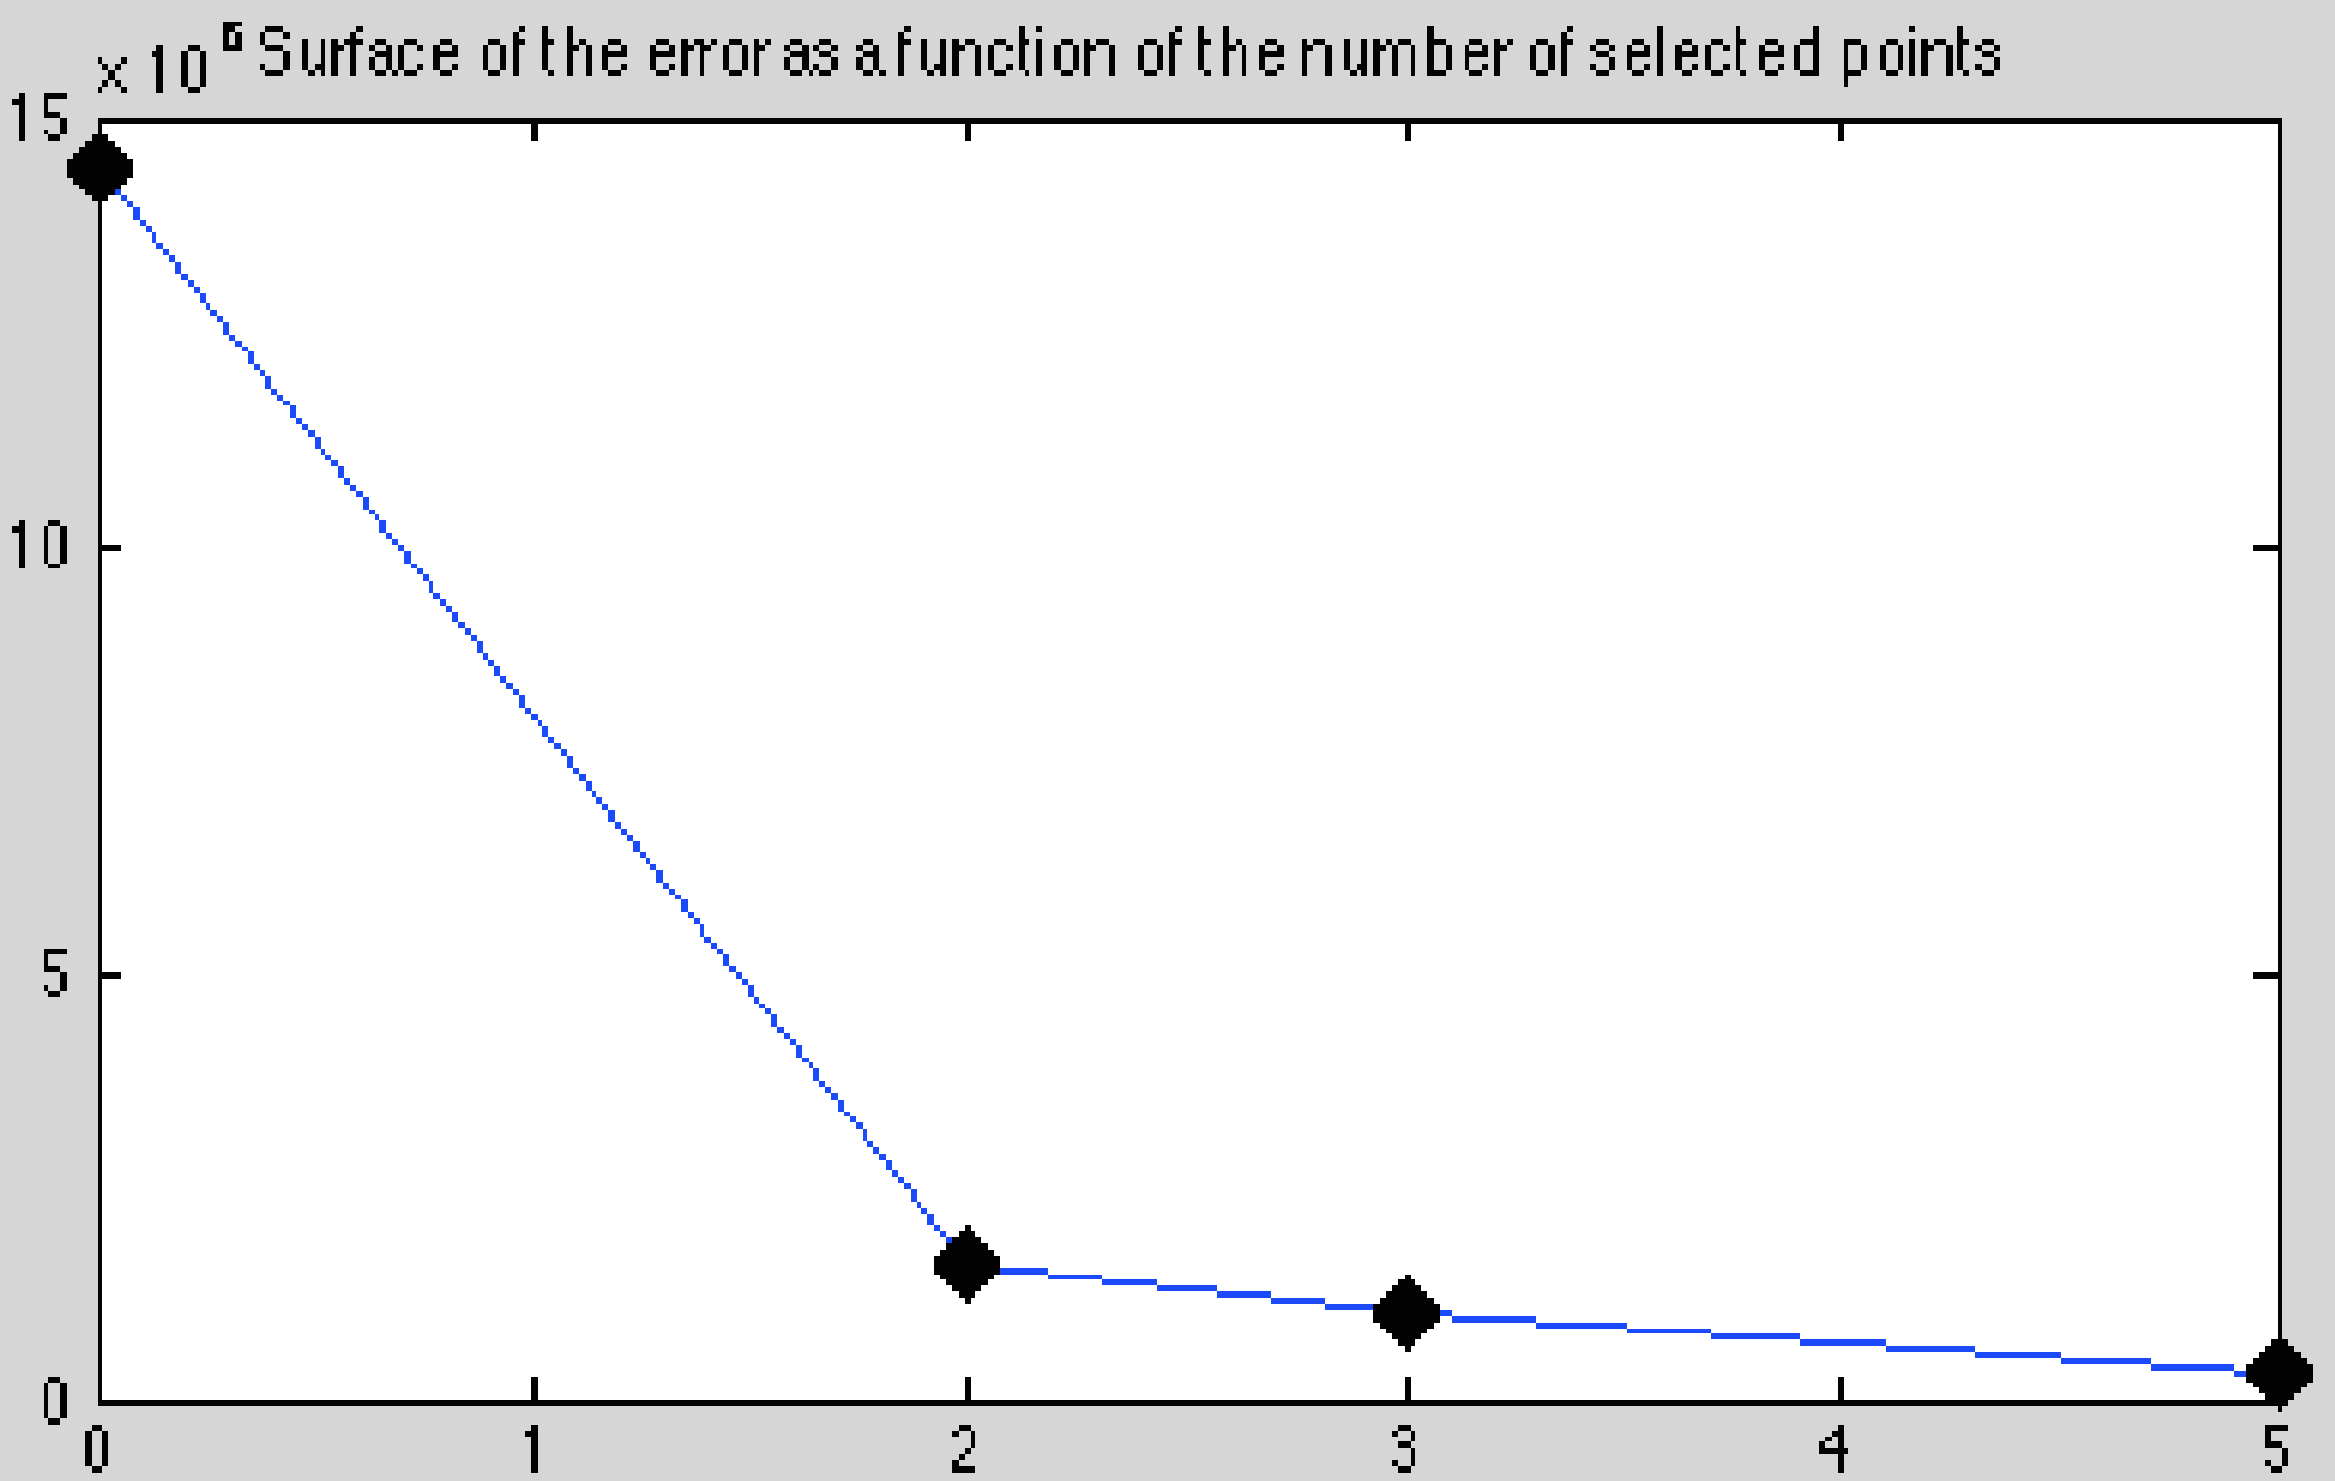
\includegraphics[trim=0cm 0cm 0cm 0cm, clip=true, height=50mm]{figch2/MC7.pdf}
}
\caption{Proxy for degrees of freedom on master curve}
\label{decreasingdegreesoff}
\end{center}
{ \small Note: The graph plots a proxy for the number of degrees of freedom for the inference of the original bid function on the number of reference points. Specifically, it plots the size of the pink shaded area in figure \ref{errorbarsasfunction} against the number of points. } 
\end{figure}

While the graphs in figure \ref{errorbarsasfunction} are displayed on inverted axes and rescaled units, we show the final master curve and uncertainty interval on the original axes and units in figure \ref{notrescaledmastercurves}. 

\begin{figure}[!ht]
\begin{center}
\makebox[\textwidth][c]{
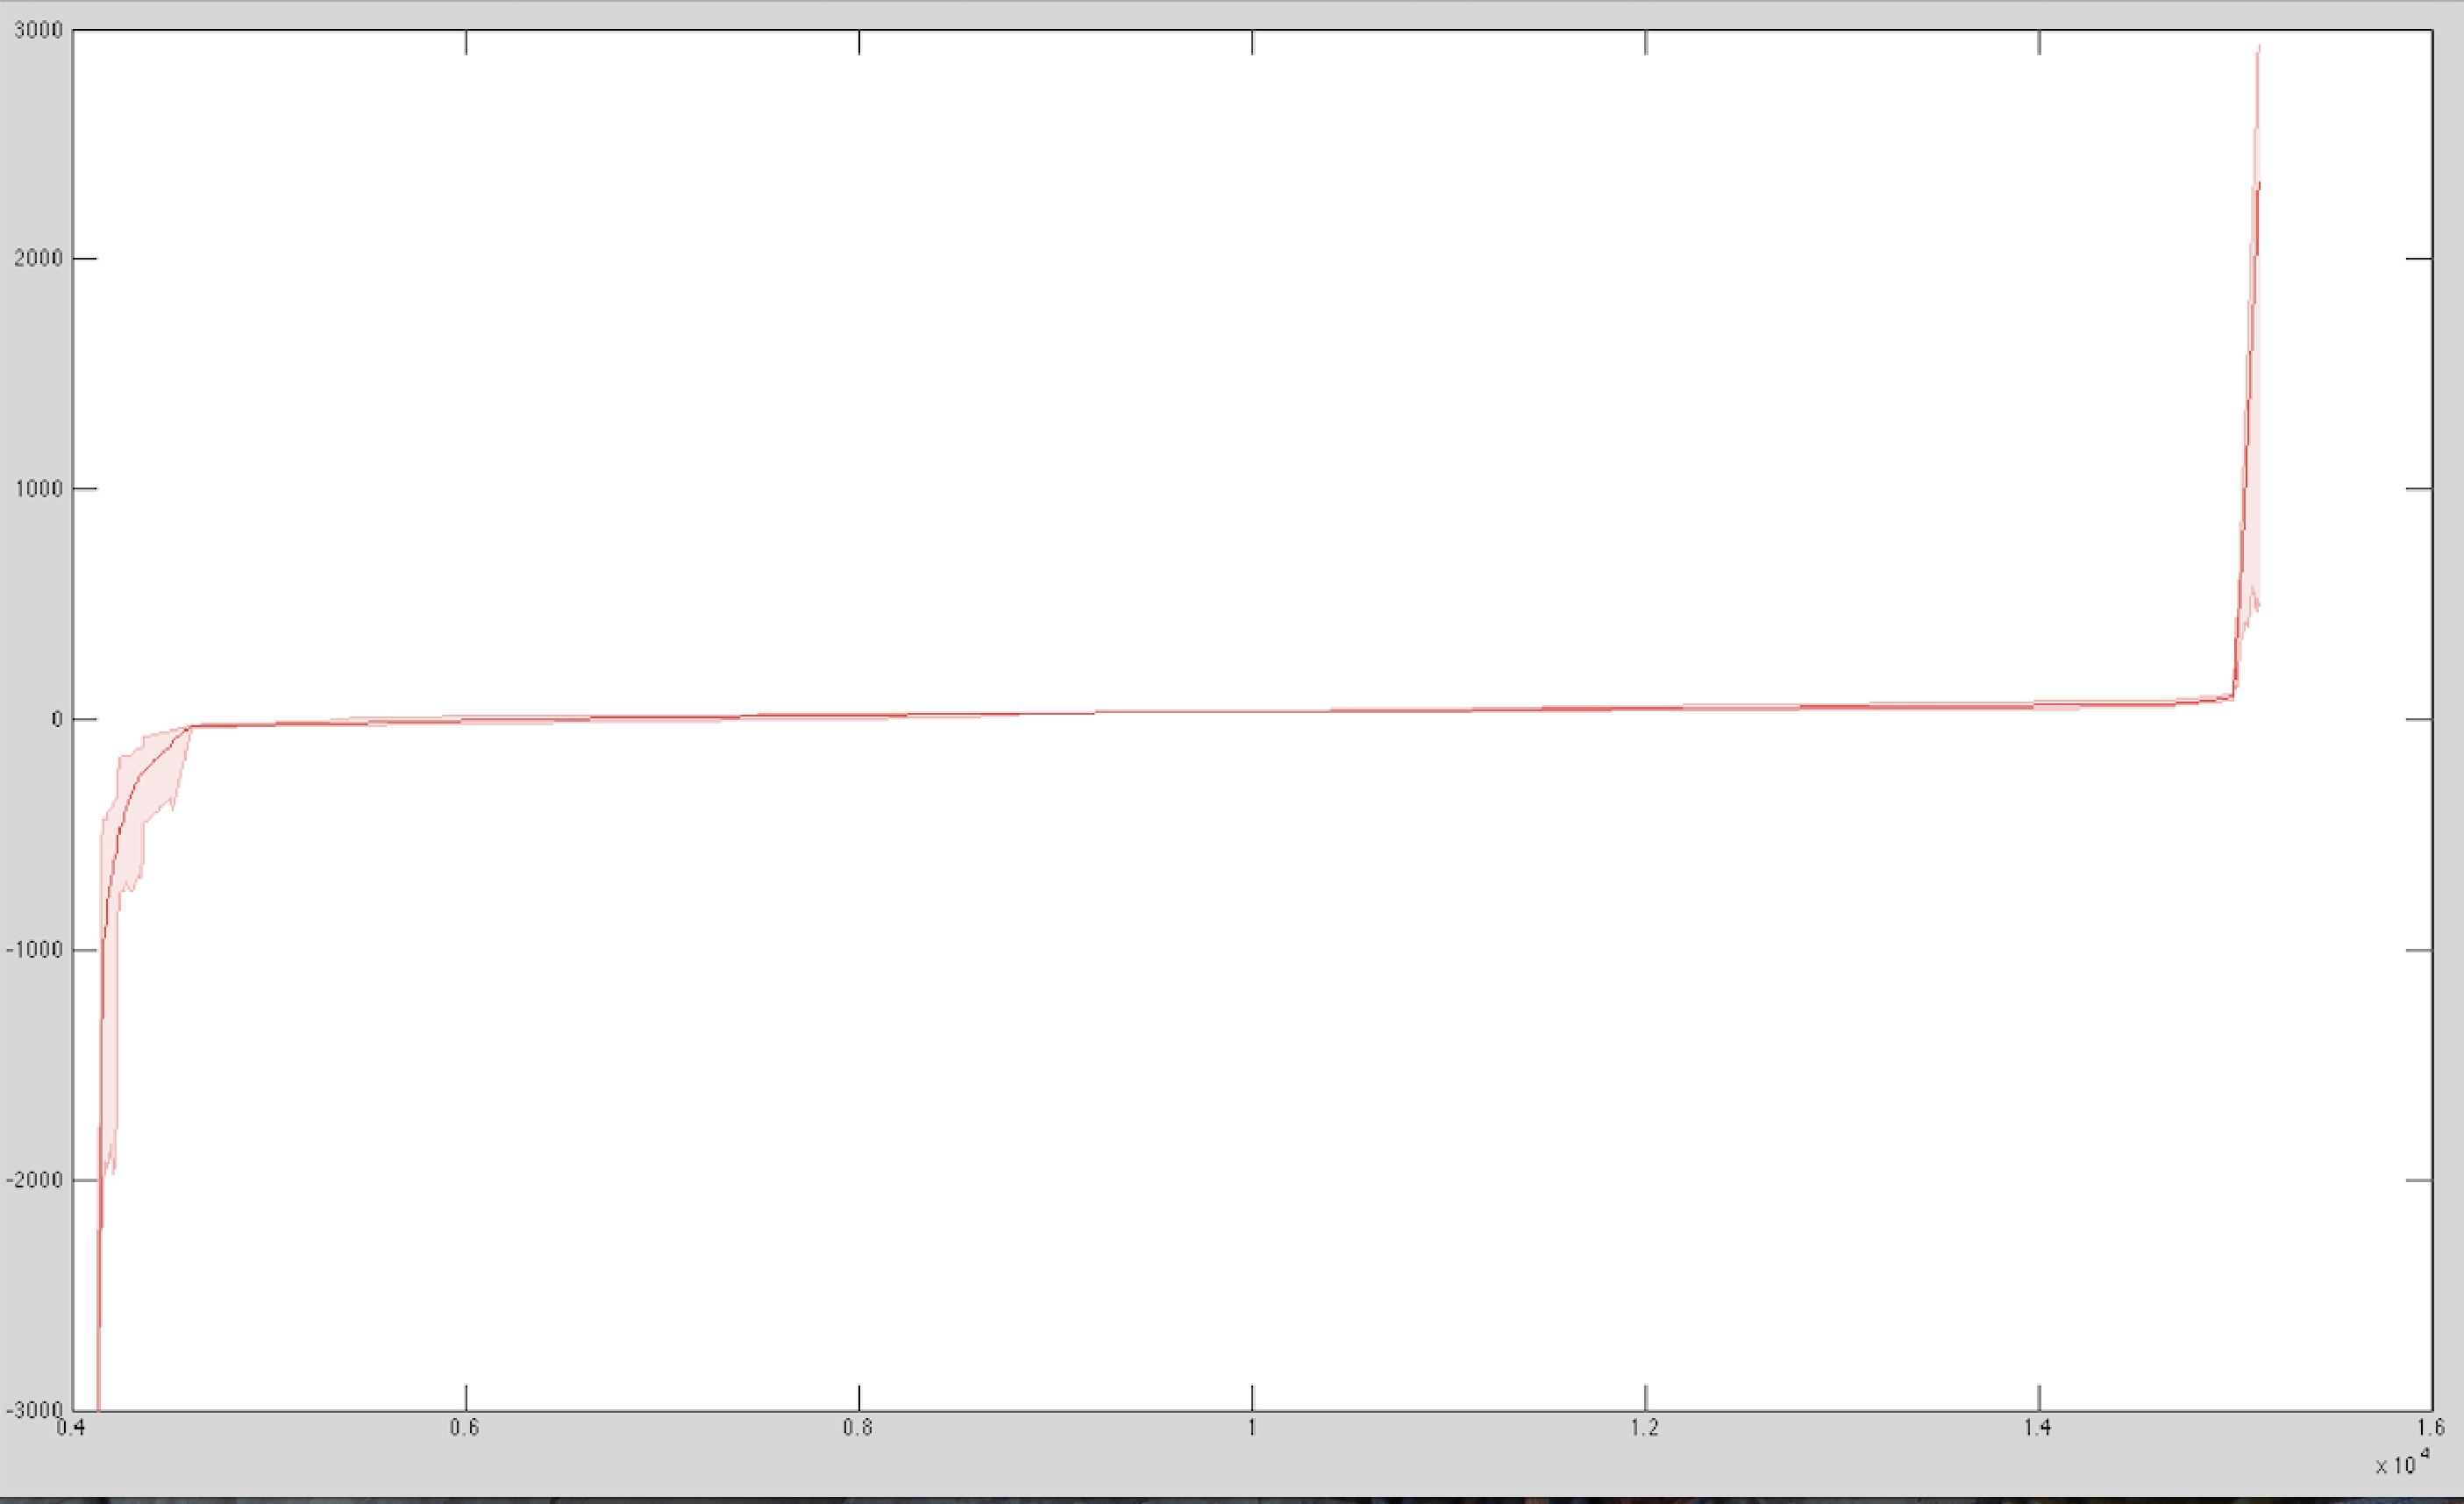
\includegraphics[trim=0cm 0cm 0cm 0cm, clip=true, height=45mm]{figch2/MC1.pdf}
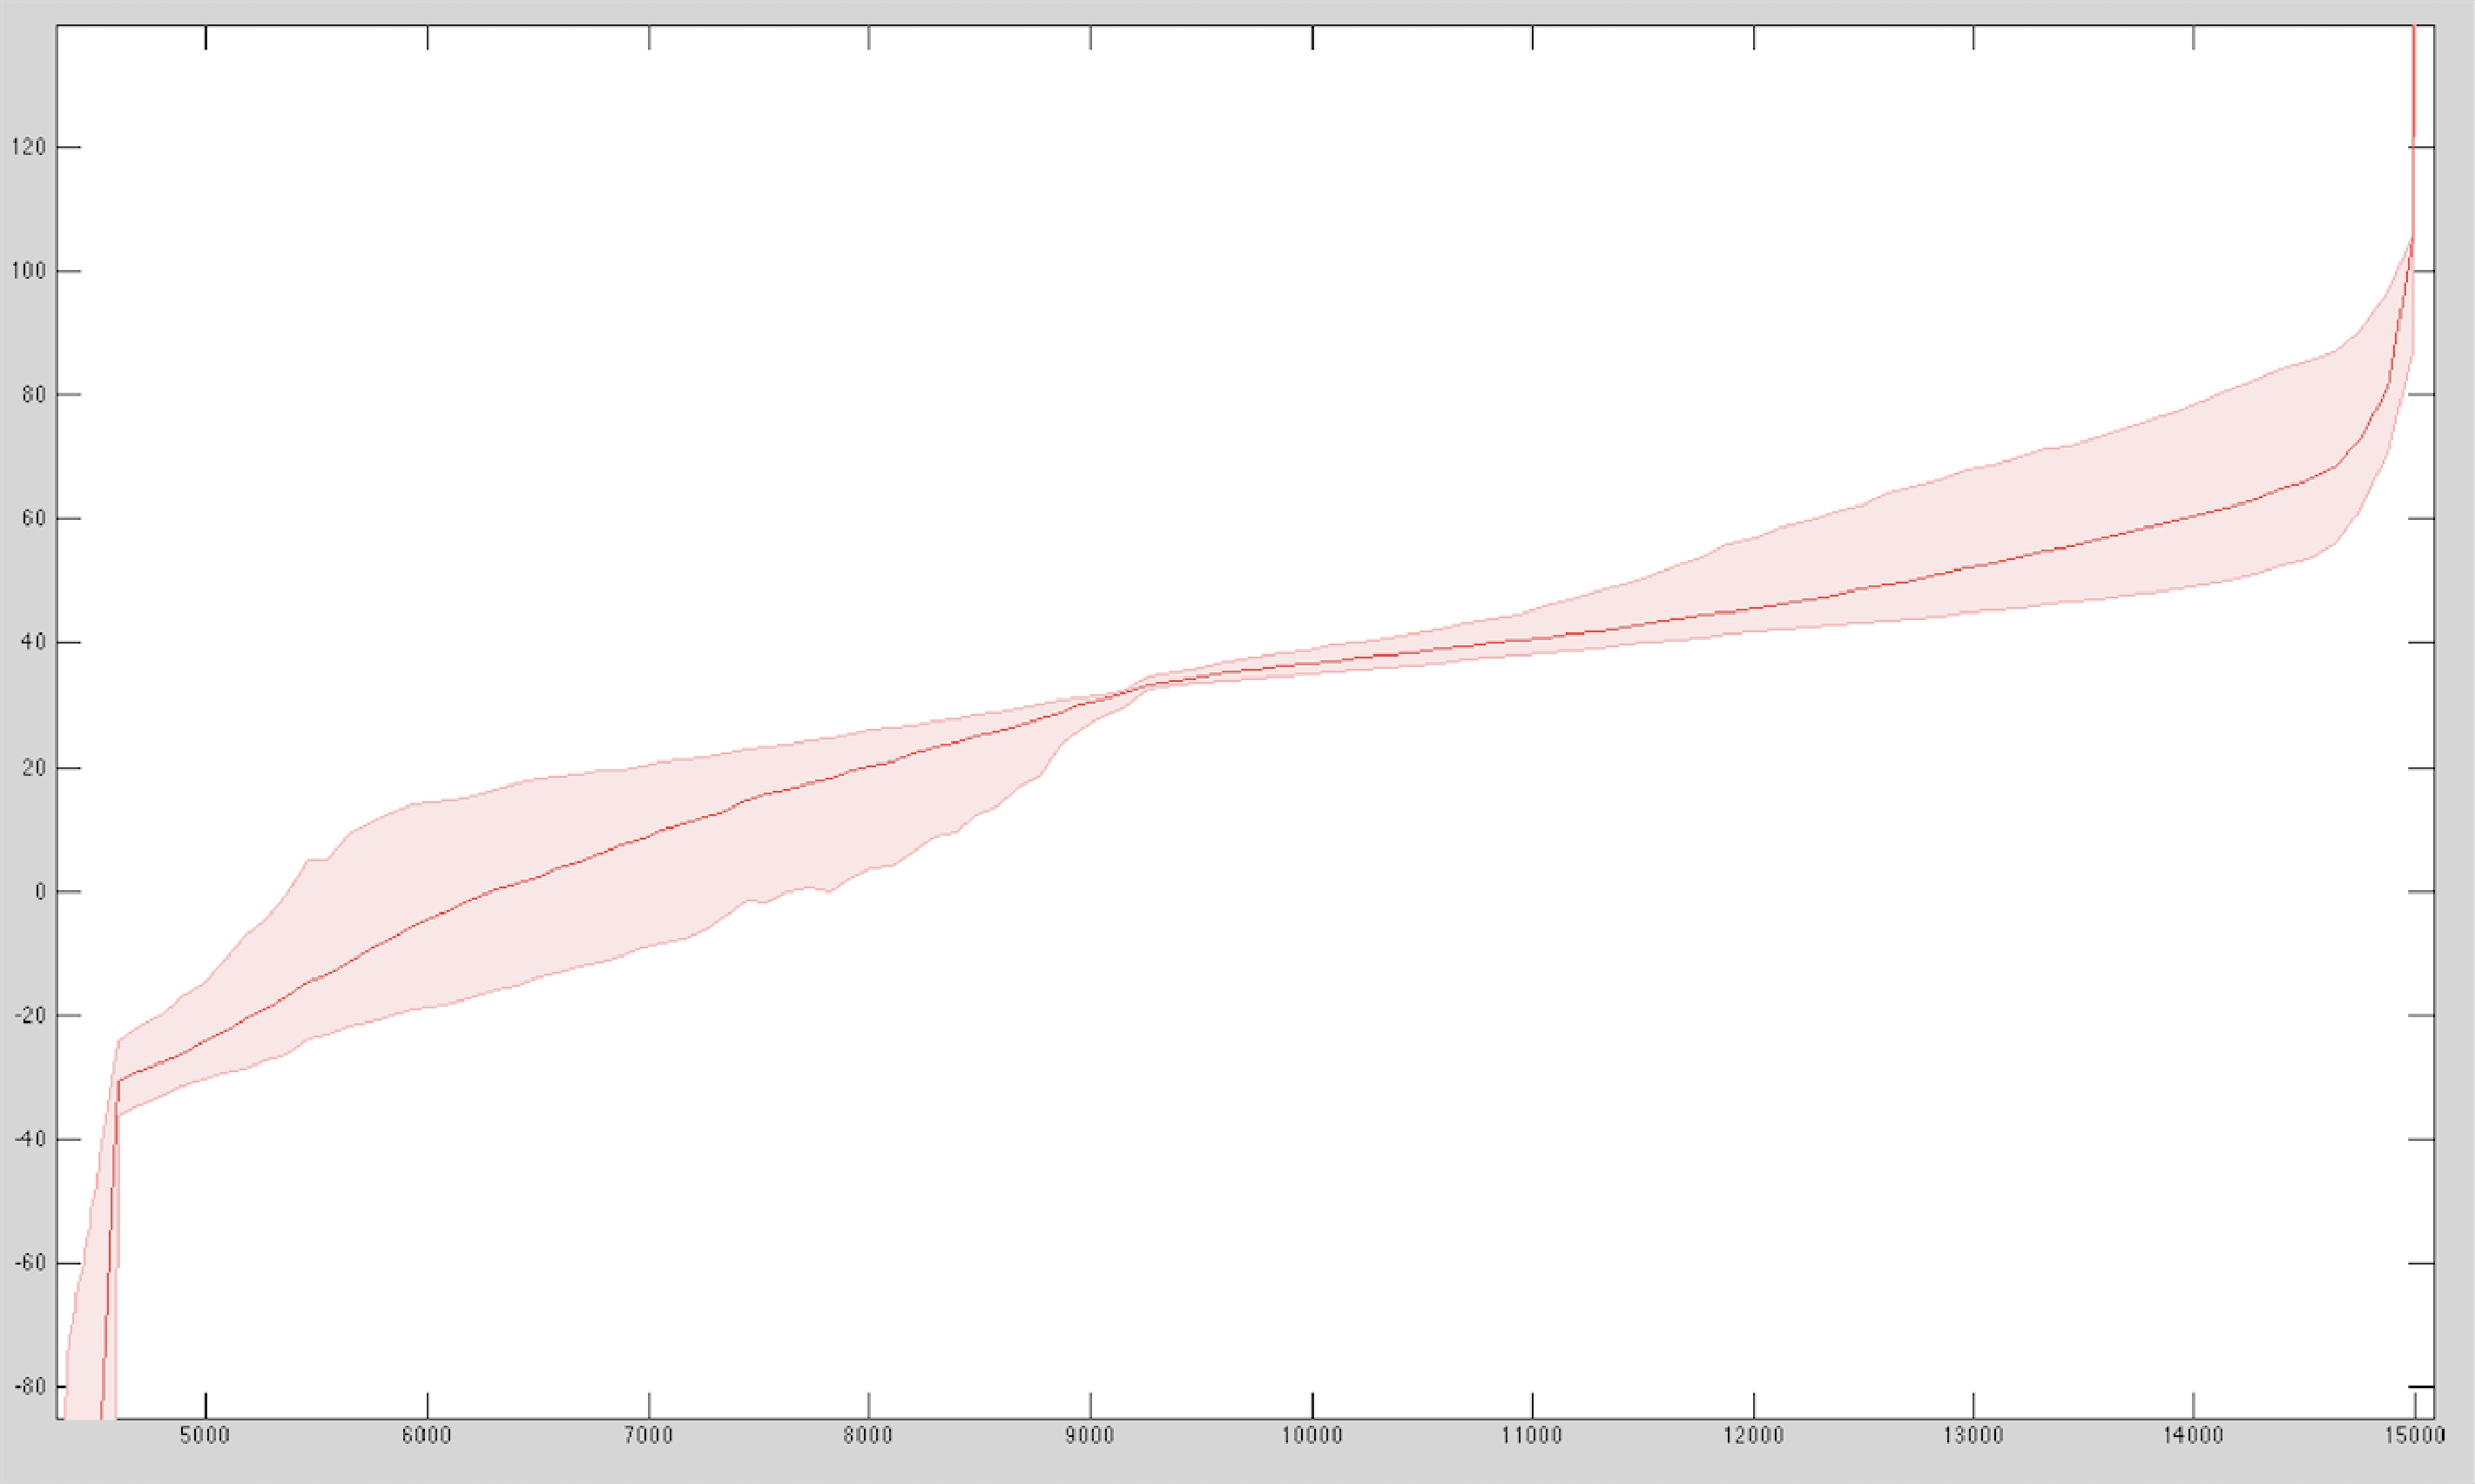
\includegraphics[trim=0cm 0cm 0cm 0cm, clip=true, height=45mm]{figch2/MC2.pdf}
}
\caption{Overall (left) and zoomed (right) Mastercurve with confidence interval}
\label{notrescaledmastercurves}
\end{center}
{ \small Note: Master curve in the quantity - price dimension.  } 
\end{figure}


\subsection{Discussion}
\label{pointccl}
In this section, we have developed an alternative technique to run a cross-section reduced form model on data generated by a market that keeps track of the full aggregate demand and/or supply functions. While we apply it to aggregate demand functions, the methodology is fit for the anaylsis of aggregate supply functions and individual bid functions of either market side.  \\

The methodology is inspired by the techniques used in the literature on Treasury auctions, but has been set up from scratch to allow treatment of more heterogenous data. Furthermore, the hard assumption of an underlying logistic function is relaxed and our non-parametric point selection avoids the storing of bid function information in the form of estimated function parameters, which are difficult to interpret. \\

Smoothing of the original bid functions is a component in both the traditional logistic function approach and our comparable point selection methodology. The smoothing enables the user to abstract of small bid function particularities and imprecision, e.g. steps in the function. However, in the traditional approach, the reduction of plus 1000 bid points into very few parameters resulted in the blurring of ``local" bid function information from all parts of the function at once. Our non-parametric approach allows specifically to control the extent to which one smoothes the underlying data through the amount of registration points considered.\\

The results of the comparable point selection are encouraging. We show that each type of point is distinctly chosen and that patterns of the original bid functions do not influence the quality of derivative information extracted at the selected points. We acknowledge the existence of bidding frictions in the original data and highlight this observation for further work. \\

\section{Methodology to aggregate geographically dispersed information on a national level}
The theoretical results of chapter 1 indicate that a key ingredient in explaining the dynamics of the bids submitted by suppliers on the electricity market is the uncertainty about demand shocks. \\

Energy  demand  addressed to the electricity markets depends on  temperature (through the heating of buildings), on wind speed (through the production of wind turbines which reduces the net demand) and on luminosity (through the production of solar panels which reduces the net demand). However, these three weather variables vary in space, whereas the market is at the national level. We introduce here the methodology with which we estimate the associated uncertainty.\\  

We have two types of meteorological data: observations and forecasts. We use both types of data to estimate the underlying uncertainty, the methodologies for each differ slightly. \\
\subsection{Dealing with meteorological data}
\subsubsection{Interpolation methodology on weather observations}
\label{interpmethodo}

Observations are obtained from M\'{e}t\'{e}oFrance for three parameters of particular interest: temperature, wind speed and light intensity. These observations take the form of tables of hourly observations for a given set of weather stations. Each parameter is observed on a different set of stations.\\ 

Due to their hourly nature, the analysis of the electricity market's sensitivity to weather requires a very high number of observations. Therefore we select between one and two stations per D\'{e}partement\footnote{There are 95 D\'{e}partement in France}, a French administrative unit of roughly 6000 $km^2$, i.e. of a typical lengthscale of about 75 $km$. We have 161 stations for temperature, 113 stations for wind speed and 106 for light intensity, as shown in Fig \ref{fig:stations}. \\


\begin{figure}[!ht]
\begin{center} 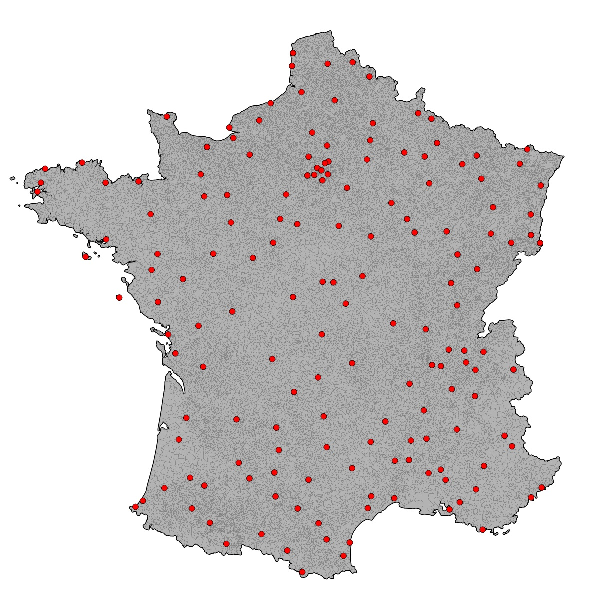
\includegraphics[height=45mm]{forqgis/stationstemp.pdf} \hspace{0.05cm}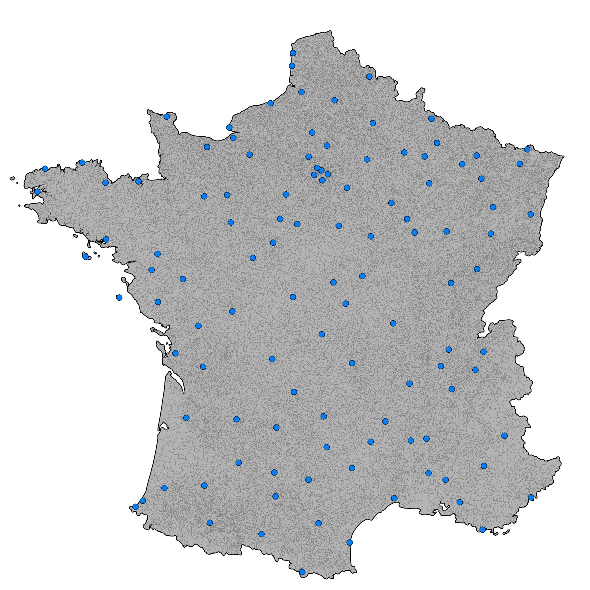
\includegraphics[height=45mm]{forqgis/stationswind.pdf}
\hspace{0.05cm}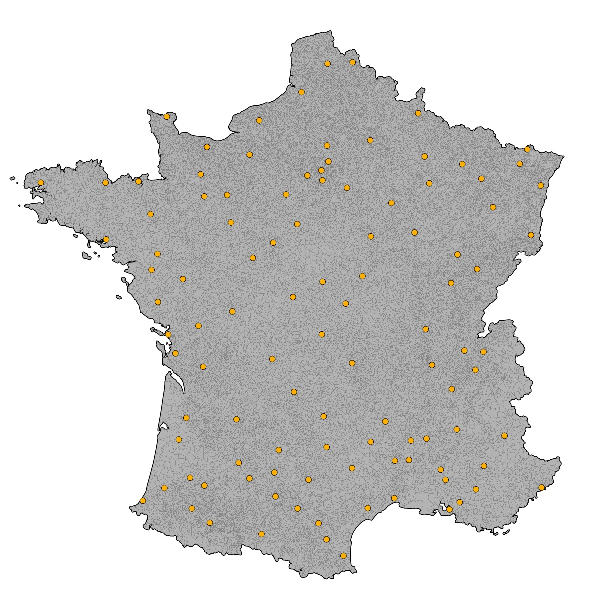
\includegraphics[height=45mm]{forqgis/stationslum.pdf}
 \end{center}
\caption{Stations for which we have hourly data. Left: temperature, center: wind speed, right: light intensity.}
\label{fig:stations}
\end{figure}

For each hour, we select the corresponding observations and interpolate them in order to reconstruct the weather on the entire French territory. An interpolation consists on inferring the value of a variable at query points using a reference data set of known values. One very important underlying assumption of interpolation methods is that of the continuity of the process underlying the data generation. The easiest interpolation method is the linear interpolation: think about a dataset of hourly observations with one missing value; to reconstruct the missing value, take the average of the value of the preceding and following hour. There are numerous methods of interpolation, even more so when the data is spatial in nature, all revolving around two main steps. First, given a query point at which one would like to infer the value of the variable, there needs to be a selection rule to know which of the points from the reference data set should be used (in our example the preceding and following values). Second, once these points are selected, one needs a weighting function to know their relative importance in order to obtain the interpolated value (in our example it is a simple averaging, that is weights of $0.5$). \\

We use the natural neighbor interpolation method, well known for its good balance between speed and accuracy. In short, in this case, the first step makes use of the Voronoi tessellation algorithm\footnote{The Voronoi tessellation algorithm takes a collection of points $\{p_k\}$ in the plane, and then partitions the plane as regions "belonging" to each point, called cells. A Voronoi cell associated with a given point $p_k$ is defined as the collection of every point in the plane whose distance to $p_k$ is less than or equal to its distance to any other $p_{-k}$. Each such cell is a convex polygon.}, one is able to define the natural neighbors of a point for which one seeks an interpolated value. These natural neighbors are used in the second step, which performs the actual interpolation as a weighted average of the values of these natural neighbors using a ratio of surfaces as weights (see Fig \ref{fig:natneighb} for more details).

\begin{figure}[!ht]
\begin{center} 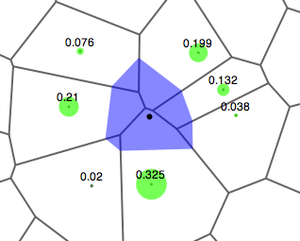
\includegraphics[height=27mm]{forqgis/natneiweights.png} \hspace{0.05cm}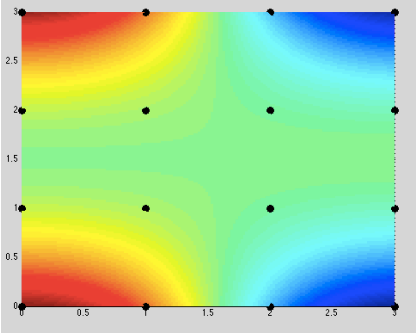
\includegraphics[height=27mm]{forqgis/natneiref.pdf}
\hspace{0.05cm}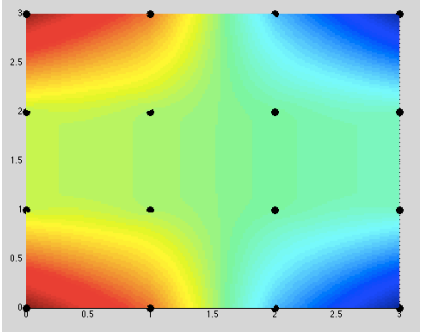
\includegraphics[height=27mm]{forqgis/natneireco1.pdf} \hspace{0.05cm}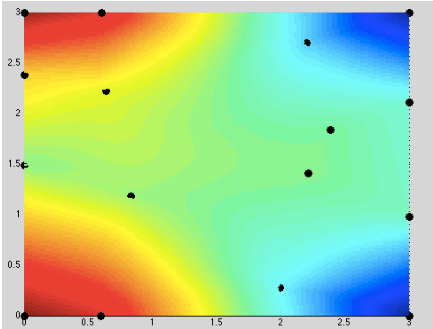
\includegraphics[height=27mm]{forqgis/natneireco2.pdf}
 \end{center}
\caption{\small Left: Voronoi's algorithm is applied once on the reference points highlighted in green to obtain the white surfaces, and a second time on the same points to which is added the query point in the center to obtain the new blue cell. The green circles, which represent the interpolating weights, are generated using the ratio of the shaded area to that of the cell area of the surrounding points. Center left: example of a reference surface (color mapped) to be reconstructed through a natural neighbor interpolation. Center right: interpolated surface with a reference set of 16 evenly organized points, represented in black. Right: interpolated surface with a reference set of 16 unevenly organized points, represented in black. From 16 points one is able to reconstruct the color mapped surfaces which are approximations of the reference one, represented in the center left image. }
\label{fig:natneighb}
\end{figure}


\subsubsection{Image transformation to recover weather forecasts}
\label{picturemethodo}

Forecasts are obtained from the Global Forecast System (GFS), and come in the form of colormaps, as shown in Fig \ref{fig:refmeteociel}. We are going to illustrate our methodology on temperature data, but the same exact approach is performed on wind speed data. The general idea is that the pointwise precision is low (2$^{\circ}C$ per color) but that the overall map contains quite a lot of information through the topology of the colored regions. We describe below how to extract this information. 
 
\begin{figure}[!ht]
\begin{center} 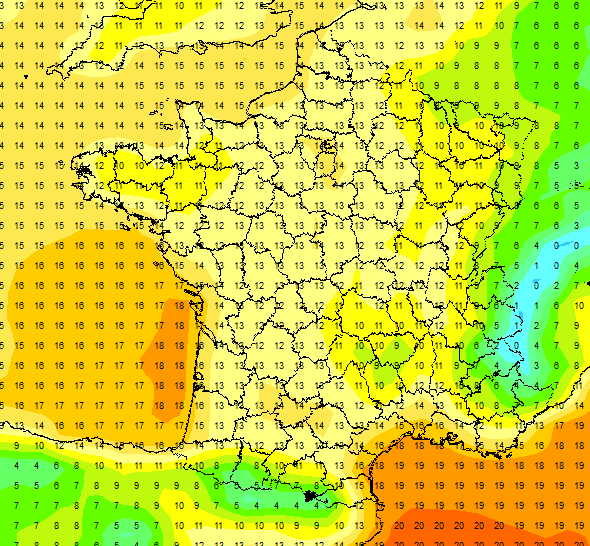
\includegraphics[height=60mm]{forqgis/ref-2011-11-03-15.png}
\end{center}
\caption{\small Temperature forecast from a simulation run by the GFS at 6 a.m. on the 3rd of november 2011, for a forecast at 22 p.m. }
\label{fig:refmeteociel}
\end{figure}

\subparagraph{First: image cleaning} To extract the relevant data we first clean the color map from its irrelevant information, namely the temperature in numbers and the administrative borders. Note that this step introduces a small amount of high spatial frequency noise, see Fig \ref{fig:mciel} left and center left. 

\subparagraph{Second: removal of redundant information} A lot of information is lost from the actual GFS simulations by using a color map representation, as temperature is described as a discontinuous variable: each color has a precision of 2$^{\circ}C$. In order to correct for this, we leverage the fact that all the information contained in this color map, that is the color at each pixel, is actually contained in a smaller set of points. Consider the value at the boundaries between different color regions: by knowing that the interior of a constant color region has a constant value, one is able to represent all the information contained in the original image by keeping only track of the values at the boundaries. To recognise those boundaries we perform image analysis, more precisely we use edge recognition methods based on finding high gradient regions, thus obtaining Fig \ref{fig:mciel} center right. 

\subparagraph{Third: surface fitting} Once we represent the information in this denser form we can perform the last step, which consists in fitting a surface to our newly defined dataset, i.e. the temperature values at the boundaries, which take the form of $(x,y,T)$ triplets. We could perform an interpolation, but these methods are not well suited to reference sets having so much structure. Here, data points lie on curves representing iso-temperatures, so that along such a curve there is a lot of data points, whereas the information is very sparse along the direction of the gradient. In addition the first step introduced some spatial noise which we want to correct to some extent: we allow our fitted surface to take different values than our data points, so as to smoothen out this noise. We define the rigidity of our fitted surface, i.e. a penalty associated to fast changes in the value of the surface, and therefore reduce the importance of the high frequency noise introduced in the first step. The end result is presented in Fig \ref{fig:mciel} right. \\

It is key to understand that this image is displayed using a colormap close to the one in the original picture to facilitate comparison but that its underlying data is continuous whereas the original image describes temperature by bins of 2$^{\circ}C$. It can therefore be used to query the value at any given point, and these values will change continuously in space instead of discrete jumps in the raw format.\\

\begin{figure}[!ht]
\begin{center} 
\makebox[\textwidth]{
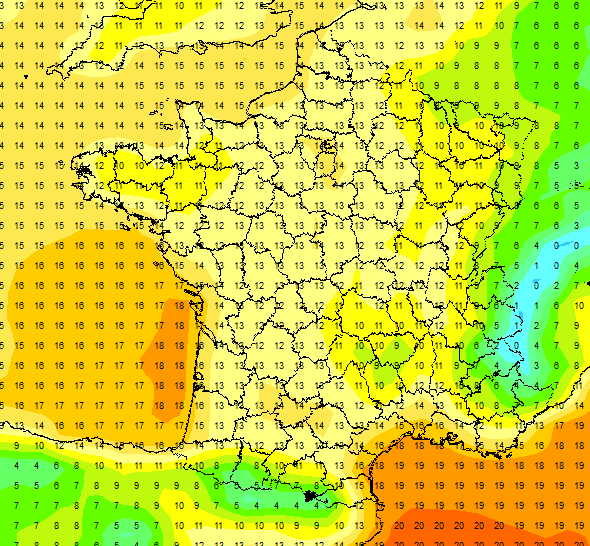
\includegraphics[height=30mm]{forqgis/ref-2011-11-03-15.png} \hspace{0.05cm}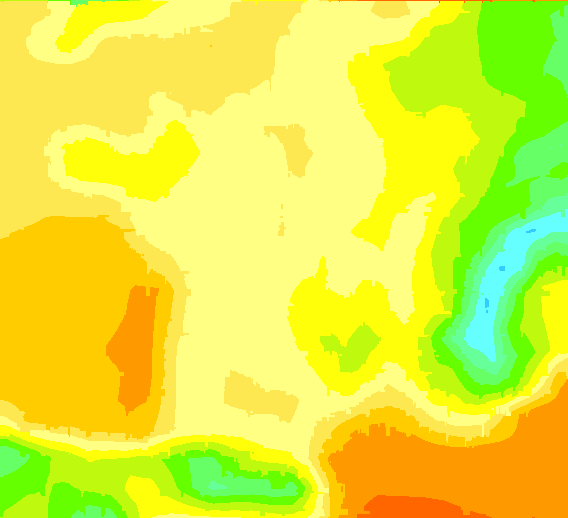
\includegraphics[height=30mm]{forqgis/2011-11-03-15.png}
\hspace{0.05cm}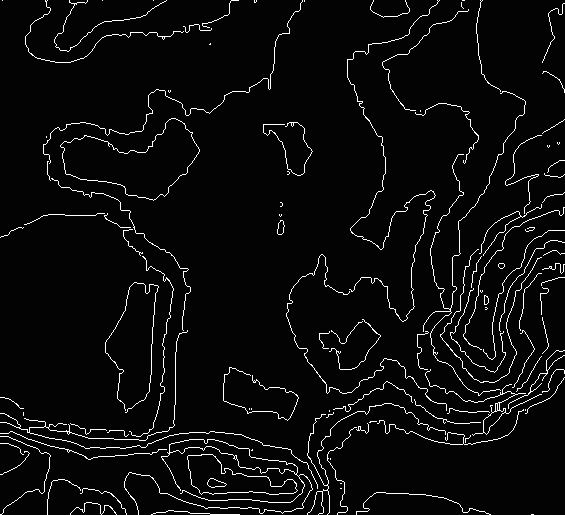
\includegraphics[height=30mm]{forqgis/mcieledge.png} \hspace{0.05cm}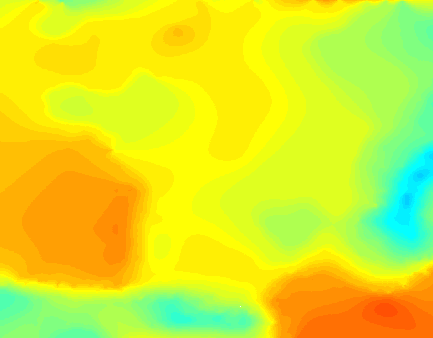
\includegraphics[height=30mm]{forqgis/mcielsmooth.png}
} \end{center}
\caption{\small Left: reference image. Center left: borders and numbers are removed. Center right: edge recognition. Right: final fitted surface. }
\label{fig:mciel}
\end{figure}

\subsubsection{Autocorrelation lengthscale}
\label{autocorr}
We use this dataset to build measures of the weather uncertainty. To do so we measure the auto-correlation lengthscale of our three weather variables of interest: temperature, wind speed and light intensity. This lengthscale measures how much are the weather variables correlated spatially. Our hypothesis is that the auto-correlation lengthscale is inversely proportional to uncertainty about the variable we are interested in. When it is small, the variable is less spatially correlated, which we interpret as being more difficult to forecast. Conversely, when the auto-correlation lengthscale is large, the variable is very correlated spatially, that is that the informational content of one datapoint is higher for the prospect of using it for the evaluation of a national effect.\\

More precisely, the argument is as follows: \\

\textbf{First}, renewable production is built by aggregating the forecast of all individual renewable sources. This means knowing the position and capacity of every renewable source, querying weather forecasts for all of these points, modeling the renewable's response to the forecasted weather, and adding the forecasted productions. \\

\textbf{Second}, we note that weather is spatially correlated, which means that the closer two points are, the closer the values for a given weather variable (the air temperature at your left hand is very close to that at your left hand, but less so across the city, and even less so across the country). This correlation roughly follows an exponential law: the difference between the values of a weather variable between two points behaves in a linear fashion for small distances, and saturates at large distances.\footnote{Intuitively, the characteristic lengthscale of autocorrelation represents the distance required between two geographical points on a map of weather forecasts to observe a decorrelation of half of its maximum value. For example on the wind speeds prediction, a characteristic length of 80 km means that if we observe two very distant points (say 1000km) to have a difference in wind speeds of, on average, 50km/h (this being the maximum difference, we are in the saturated regime), then we will observe, on average, wind speed differences of 25km/h for points distant from each other by 80km.} The transition between those two regimes is given by a caracteristic lengthscale, a bit less than 200km on average. \\

\textbf{Third}, we observe that the average distance between production points is large enough that the relevant regime of autocorrelation is the saturated part.\footnote{For N production points, we compute the N(N-1)/2 pairs of points, consider their distances, and compute the average of these distances weighted by the production capacity at every point. In the case of the wind we have an average distance of 459 km, in the case of the photovoltaic production we have an average distance of 499km.} \\

\textbf{Fourth}, we note that there are two main channels through which the overall uncertainty about renewable production is related to the weather. There is an issue of error averaging, which means that if the weather becomes very spatially uncorrelated, one can expect errors to cancel out relative to a given bias in the forecast. This channel would tend to imply that more spatial variations imply a smaller uncertainty about production. There is also the issue that weather forecasts are numerical simulations and that the mesh size for such simulations, typically 5km for the high precision ARPEGE model of Météo France, implies that the errors are higher as the simulated phenomenons have higher gradients. This means in our case that the uncertainty about the forecast increases as the weather becomes more spatially uncorrelated. \\

\textbf{Fifth}, these two effects are of opposite signs, but our third point is an argument for considering that the averaging of errors is smaller than the simulation errors. Therefore we expect our uncertainty to increase as the spatial autocorrelation decreases (i.e. more spatial variation). \\

This can be summed up with the following hand-waving argument: when there is more spatial variations, the weather is more messy, therefore more difficult to predict. \\

To understand what the autocorrelation lengthscale captures, take two points on a plane and a spatially correlated bounded variable. If those points are infinitely distant, the value of the variable at these points should be uncorrelated. That is that the absolute difference between the variable taken at those two points should have a given average value. Conversely, two points infinitely close should have the same value, i.e. a zero absolute difference between the variable taken at those two points. The question is how fast is the transition between those two limit cases. First, we define the average absolute difference between two points when distant of a given value. Second we extract a typical lengthscale. \\

To define the average absolute difference between two points when distant of a given value, we consider at a given point in time every possible pair of points in our dataset. For a given pair we compute its distance and its absolute difference in value (in black in Fig.\ref{figautocorrel}). For 100 datapoints we obtain 4950 pairs. We then use a kernel smoother in order to obtain the average non parametric autocorrelation function (in blue in Fig.\ref{figautocorrel}). \\

To recover a typical lengthscale we make the parametric assumption that the auto-correlation is exponential in nature. We fit an exponential function through our smoothed data (in red in Fig.\ref{figautocorrel}), and recover the exponential decay parameter as our lengthscale (in green in Fig.\ref{figautocorrel}). We perform this operation for every hour in our dataset and every weather variable. The results are timeseries for the characteristic lengthscale of the weather parameters.


\begin{figure}[!ht]
\begin{center} 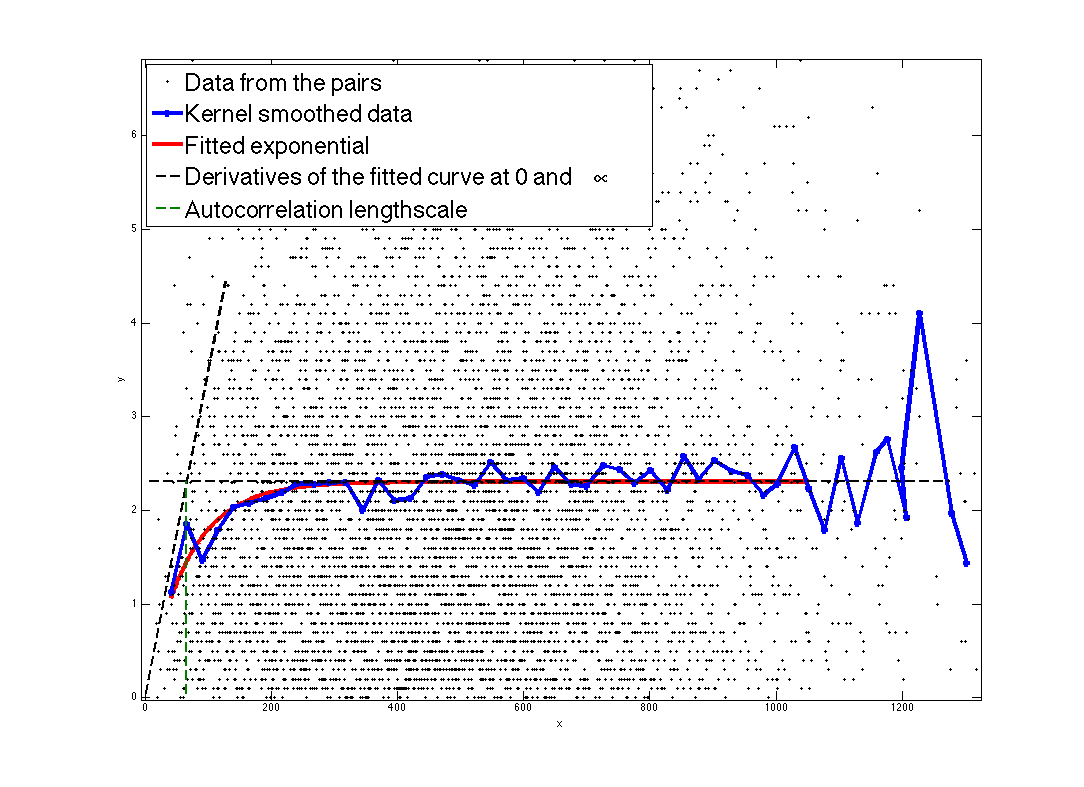
\includegraphics[height=95mm]{forqgis/lautocorgraph.png}
\end{center}\vspace{-0.9cm}
\caption{Auto-correlation lengthscale computation. In black are the points obtained from all the pairs from our original data, that is absolute wind speed differences as a function of the distance between the two points. In blue is the kernel smoothed function from those points. In red is the exponential fit. In black are the derivatives of the fit at $0$ and $\infty$. In green is the recovered auto-correlation lengthscale. The unit for the lengthscale is in km.}
\label{figautocorrel}
\end{figure}

\subsection{Aggregation of local information}
\subparagraph{Wind1DA}
\label{Wind1DA}

\textit{Wind speed (average speed in km/h):} 
\label{winddetail}
Wind speeds influence the productivity of wind turbines, which are a source of unreliable electricity generation. In general, renewable technologies benefit from a feed-in guarantee by the state. That is, regardless of the trading outcome on all markets, renewable energies will be the first to be fed into the power grid at a guaranteed price. \\

Consequently, the electricity production of renewable technologies represents a production shock for all actors on the market. The production shock means that the demand to be served by traditional electricity producing firms is reduced by the amount that is serviced by the electricity gained from renewable sources. \\

In the case of wind turbines, the average speed of the wind per hour allows to proxy for the size of the production shock due to the electricity generation from wind energy. \\

We use hourly windspeed forecast in the form of color maps from the Global Forecast System (GFS), giving the speed by bin of 5 km/h at 10m above ground, and the location and production capacity of the wind turbines present on the French territory, given by the SOeS (service d'observations et d'études statistiques - observations and study department) a department of the French environment ministry. \\

We consider that all turbines in France are of the same type, that is that they have the same response curve and height. \\

A typical response curve is represented in Fig. \ref{fig:typpowercurve}. It has three main characteritics: the wind speed at which the turbine starts to produce electricity, called the cut-in speed, the speed at which the turbine reaches its rated output, called the rated ouput speed, and the speed at which the turbine has to stop to avoid damage, called the cut-out speed. We use data publicly available\footnote{http://www.thewindpower.net } to obtain a rough estimate of the French average wind turbine characteristics. We use a cut-in speed of 2.5 m/s, a rated output speed of 14 m/s, and reduce arbitrarily the cut-out speed from an estimate of 24 m/s to 20 m/s to account for the fact that a turbine is shut down not when the average speed is too high but when the maximal speed becomes dangerous for the turbine.\\ 

Wind speed also increases with height, and turbines are typically between 60 and 80m high. We therefore apply a multiplier to the reconstructed wind speed at 10m. \\

We seek to reconstruct the French wind energy production from meteorological data. The two adjusted values, the cut-out speed and the speed multiplier, are adjusted by hand to obtain reasonnable fits. The reason for this is that the reconstruction of wind speed and aggregate production is computationnally intensive, therefore we cannot perform a full blown estimation. We choose these values with a precision of roughly 10\% with repect to their admissible range of values. \\

\begin{figure}[!ht]
\begin{center} 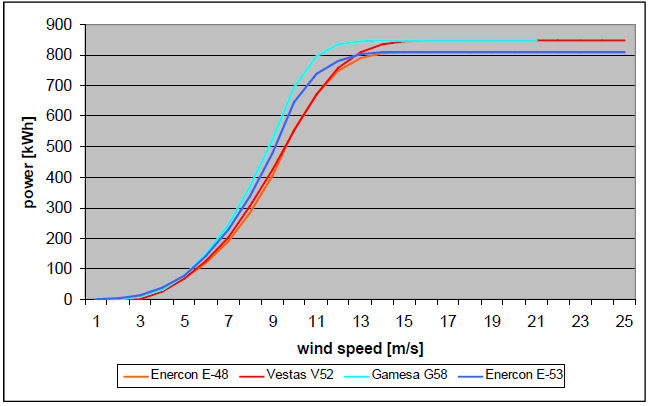
\includegraphics[height=50mm]{forqgis/ref-powercurve.png}
\end{center}
\caption{\small Typical response curves of different wind turbines}
\label{fig:typpowercurve}
\end{figure}


We obtain a reconstruction of wind production from day-ahead wind speed forecasts that we compare to actual observed production and to day-ahead wind production forecast computed by RTE, the French grid operator as shown in Fig.\ref{fig:windreco1DA}. We stress here that our aim is two-fold: to link wind turbines' production to weather data and to use forecast data as the market actors only possess this information when bidding. We do not aim at producing better forecasts than the grid operator, the figure is only displayed to show that our methodology produces reasonable estimates (we obtain a correlation coefficient between our forecast and the observation of $0.85$ where the grid operator obtains $0.97$).  

\begin{figure}[!ht]
\begin{center} 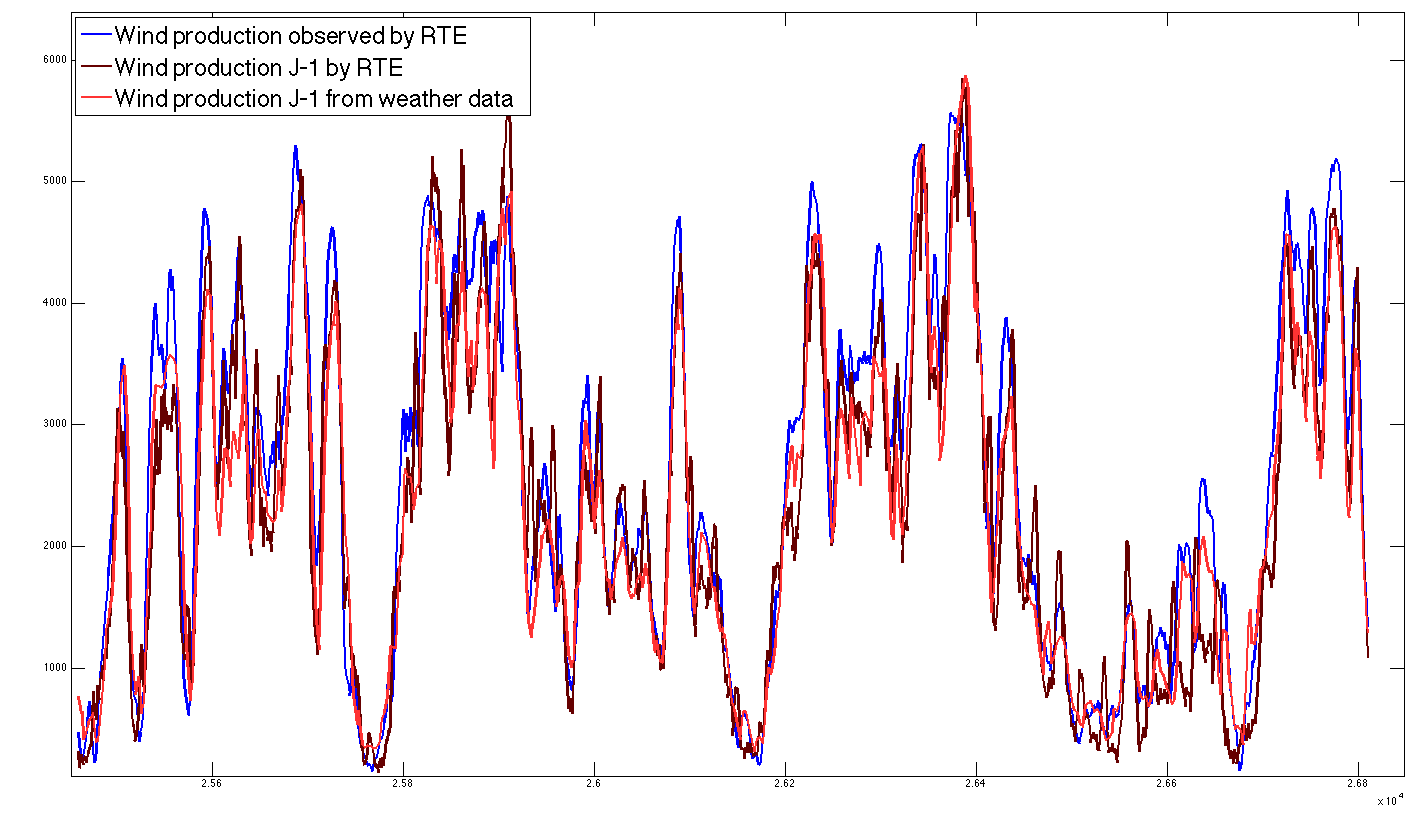
\includegraphics[height=80mm]{forqgis/windprodD1A.png}
\end{center}
\caption{\small All curves are hourly production data. The origin of the hours is the first of January 2011, and the production is in MWh. In blue: the observed wind production. In dark red: the day-ahead predictions from the grid operator. In light red: the day-ahead predictions from weather data.}
\label{fig:windreco1DA}
\end{figure}


\subparagraph{Tempeff15}
\label{Tempeff15}

We focus on the effect of temperature on the demand of electricity first. In France, a high percentage of the population heats their housing with electricity, therefore cold waves have a high impact on electricity consumption: 2300MW of additional power consumption for every drop of 1$^\text{o}C$ below 15$^\text{o}C$, as shown in Fig.\ref{elecconstemp} sourced from \cite{rtewebsite1}, the French grid operator. \\

\begin{figure}[!ht]
\centering
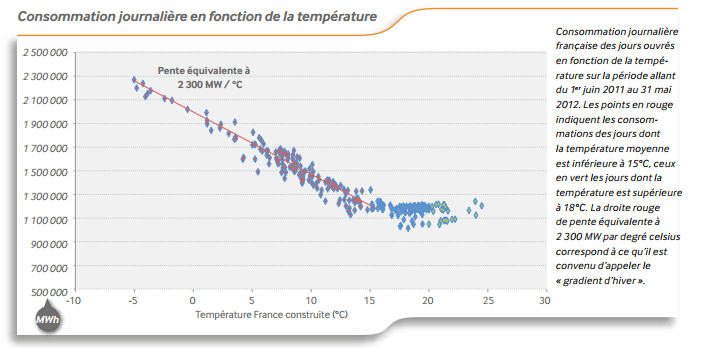
\includegraphics[height=65mm]{forqgis/Temp_Cons_France_RTE.png} 
\caption{Daily electricity consumption in France as a function of the temperature, \cite{RTEbilan2012}}
\label{elecconstemp}
\end{figure}


We apply this information to our observed meteorological data in order to build an effective temperature for France aimed at capturing its effect on consumption. To do so, we reconstruct temperature data for every French \emph{commune}, the smallest administrative unit in France (there are around 36000 of those). We consider population as being a good proxy for potential heat consumption, therefore we apply it as a weight to the \emph{commune} temperature. Lastly, we consider that temperatures saturate at $15^\text{o}$C. This allows us to build an effective temperature taking into account where the population is located and the nonlinearity of heat start up which in turn allows us to account at the country-level for the local impact of temperature on the electricity consumption.  \\

\subparagraph{Solar}
\label{Solar}
Light intensity (in $W.m^{-2}$) impacts the electricity market through multiple channels. The most obvious one is the associated electric production from photovoltaic panels. But there is another channel through which lighting can be seen as impacting electricity consumption: more sunlight decreases artificial light usage. In France, annually, the electric consumption that can be attributed to lighting represents roughly 50 TWh where solar production is roughly 4 TWh.\footnote{These estimates are computed by the authors based on numbers coming from \cite{eleceurope}, INSEE and EDF} \\

We have photovoltaic production data, which in itself is a blackbox. As we aim to link meteorological data to consumption we first want to validate the quality of our meteorological data. To do so we reconstruct the photovoltaic production from weather data. We know what are the hourly luminosity conditions on the French territory but also where is installed the photovoltaic production capacity. The SOeS (statistical observation and study department), a branch of government, publishes each year a file containing the installed capacity of renewable energy sources per communes, a French administrative unit with a typical size of roughly 3 $km$. \\

We use observed luminosity data from M\'{e}t\'{e}oFrance, as there is no hourly forecast of luminosity, and assume a sigmoid response from photovoltaic panels to light intensity with a saturation towards high light intensity, that is approximately a linear response up to a certain threshold. The results are shown in Fig.\ref{solarreco}.  \\

\begin{figure}[!ht]
\centering
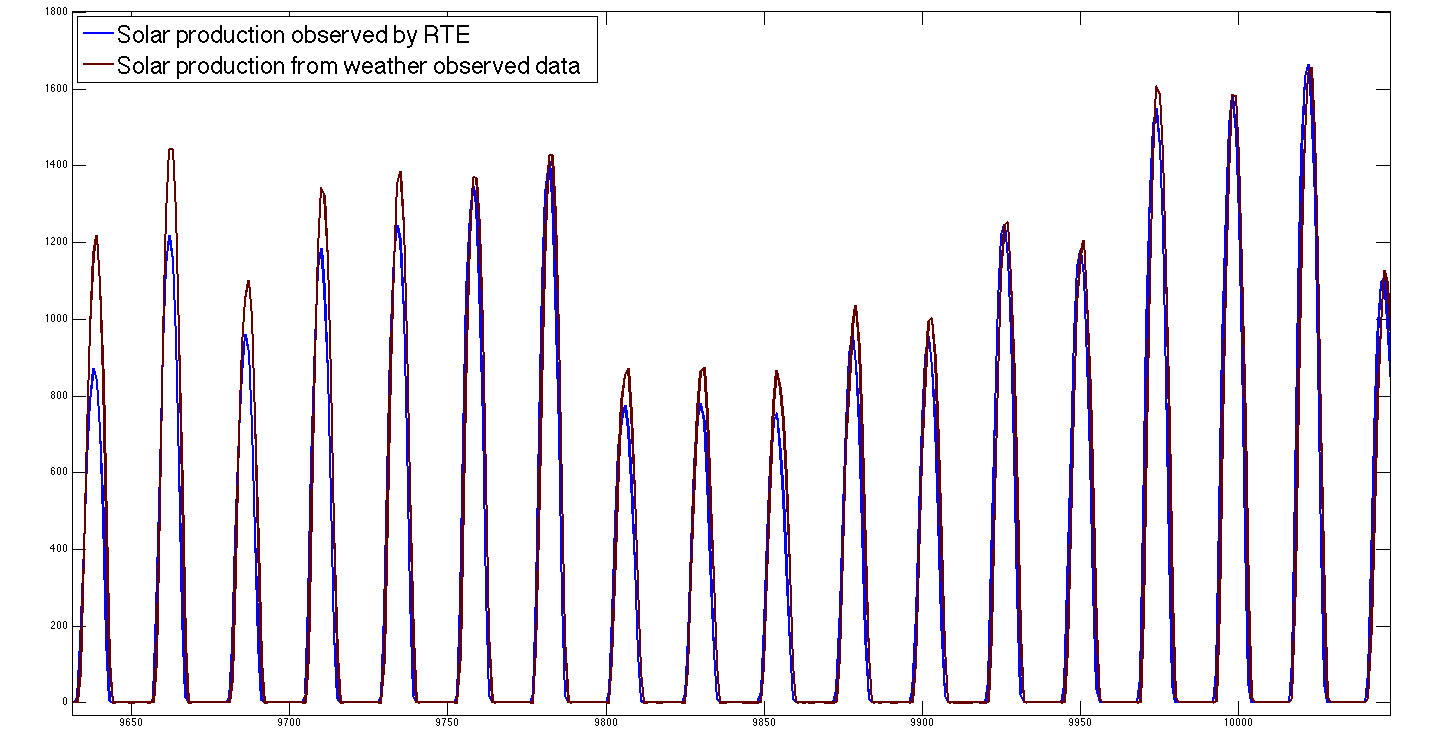
\includegraphics[height=65mm]{forqgis/solobs_reco.png} 
\caption{Hourly solar production in MWh. The time origin is the first January 2011. In blue: observed production by RTE. In dark red: reconstructed production from observed weather data.}
\label{solarreco}
\end{figure}


We observe that solar production is much more regular than wind production, therefore it is not possible to build a proxy for lighting consumption that would allow us to decorrelate the effects from production and lighting. We therefore stick to this proxy to capture the net effect of both channels.

\subsubsection{Other controls}
\subparagraph{Tempeff}
We also build an effective temperature that does not account for the nonlinearity at $15^\text{o}$C following the same methodolgy otherwise as a control. 


\subparagraph{Roll\_Temp$H$}
\label{rolltemp720}
Variable capturing seasonal trends by using the rolling average temperature on effective temperature (Tempeff15) over the last $H$ hours.

\subparagraph{Roll$_{avgTH}$} Variable capturing seasonal trends by using the rolling average temperature on temperature Tempeff (no kink) over the last H hours, i.e. the last H/24 days.

\subparagraph{suncycle}\label{suncycle} Variable capturing intraday seasonality be measuring the intensity of sun- light as a percentage of the maximum daily observation. Midday is defined at the maximum sun intensity every day, i.e. Midday = max(Solar). Thus, suncycle$_H$ = Solar$_H$ / Midday.

\subparagraph{deltasun}\label{deltasun} Variable computed to proxy for dusk and dawn. It is computed as the absolute difference between suncycle$_H$ - suncycle$_{H−1}$.

\subparagraph{SolarRest}
\label{SolarRest}
Solar represents estimates of solar production. Therefore, it is highly collinear to the daily suncycle variable since solar production is light dependent. %Furthermore, the sun is closer to the French earth in summer, thus it is also correlated to seasonal trends represented by Roll\_Temp720. 
SolarRest is the residual from a regression of Solar on suncycle %and IT1, where IT1 is an interaction variable of suncycle and Roll\_Temp720. 
and captures the unexplained part of solar production on top of pure light intensity considerations. Table~\ref{SolarBlack} gives the results of the regression.
\begin{table}[H]
\begin{center}
\begin{tabular}{lcc} 
%\toprule
 & (1) &  \\
% & Black\_3 &  \\
\textcolor{white}{VARIABLES} & Solar & SE \\ \midrule
\vspace{4pt} & \begin{footnotesize}\end{footnotesize} & \begin{footnotesize}\end{footnotesize} \\
suncycle & 1,500*** & 3.903 \\
Constant & 0.876** & 0.383 \\
%\vspace{4pt} & \begin{footnotesize}\end{footnotesize} & \begin{footnotesize}\end{footnotesize} \\
\midrule Observations & 150,959 &  \\
 $R^2$ & 0.702 &  \\ \bottomrule
\multicolumn{3}{c}{\begin{footnotesize} *** p$<$0.01, ** p$<$0.05, * p$<$0.1\end{footnotesize}} \\
\end{tabular}
\end{center}

\caption{\label{SolarBlack} Regression of Solar on suncycle}
%\emph{Note}: ****TBC
\end{table}

\subparagraph{RteBlackBox}
\label{RteBlackBox}
%\subparagraph{RTE's one day ahead prediction of total consumption:} 
RTE, the French grid operator gives day ahead predictions of the total hourly consumption, which are available at the time of bidding. This variable is called PrevConsoH. \\

We do not have access to the exact definition of the index and it is thus a black box. However, it is available to the firms at the time of bidding and we want to include it in the demand estimations. \\

At the same time, it is evident that this variable uses much of the information that we explicitly control for in the regressions, the variables defined above, therefore in addition to the possibility that we might not have all the variables that go into building this prediction for the hourly consumption, collinearity is an issue. In order to have correct coefficient estimates, we adopt an instrumental variable approach by regressing the RTE prediction on our exogenous factors, extracting the residuals and only including the unexplainable component of the RTE prediction in the demand estimation in the form of a separate variable called RteBlackBox.\\

Formally, RteBlackBox is equal to the predicted residuals ($u$) of the following regression, where $X$ stands for the vector of explanatory variables: Tempeff15,  Roll\_Temp24 ,  Roll\_Temp240, suncycle, morning, deltasun and EWH.  \\
\begin{equation}
\label{blackreg}
 \text{PrevConsoH} = a + bX +u 
\end{equation}
In table \ref{black1} we give the output of regression \ref{blackreg} in column $1$, which is strong support that our prepared data for exogenous variables is of very high quality. We highlight the significance of all explanatory variables at the $1\%$ level and the R$^2$ statistic of $85.3\%$. \\

\begin{table}[!ht]
\begin{center}
\begin{tabular}{lcc} \toprule
 & (1) & (2) \\
% & Black\_1 & Black\_1 \\
\textcolor{white}{VARIABLES} & PrevConsoH & PrevConsoH \\ \midrule
%\vspace{4pt} & \begin{footnotesize}\end{footnotesize} & \begin{footnotesize}\end{footnotesize} \\
Tempeff15 & -682.6*** &  \\
Roll\_Temp24 & -802.0*** &  \\
Roll\_Temp240 & -1,175*** &  \\
SolarRest & -0.860*** & -0.345*** \\
suncycle & 7,849*** & 7,418*** \\
morning & -4,759*** & -4,398*** \\
deltasun & 10,108*** & 9,010*** \\
EWH & -1,245*** & -1,254*** \\
Tempeff &  & -301.4*** \\
Roll\_avgT24 &  & -687.3*** \\
Roll\_avgT240 &  & -918.2*** \\
Constant & 77,701*** & 76,651*** \\
%\vspace{4pt} & \begin{footnotesize}\end{footnotesize} & \begin{footnotesize}\end{footnotesize} \\
\midrule Observations & 146,909 & 146,909 \\
 $R^2$ & 0.853 & 0.816 \\ \bottomrule
\multicolumn{3}{c}{\begin{footnotesize} *** p$<$0.01, ** p$<$0.05, * p$<$0.1\end{footnotesize}} \\
\end{tabular}
\end{center}

\caption{\label{black1} "Black box" regression on RTE predicted consumption}
\emph{Note}: The dependent variable PrevConsoH is the day ahead prediction by RTE of the total consumption in France. 
%**** Gives units on variables to interpret SE. 
%*** Maybe remove SE colums. 
\end{table}

We highlight that the comparison of columns 1 and 2 gives very strong support to our adjusted measure of effective temperature (Tempeff15 instead of Tempeff), which takes into account the demand behaviour as a function of the temperature. Temperatures above $15^o$C are considered not to impact demand behaviour \cite{rtewebsite1}.

\section{Conclusion}

In this methodological chapter we present the different methods that we developed to study in the next chapter the impact that uncertainty about demand shocks can have on suppliers' bids. \\

We want to be able to describe how bids change shape as a function of a number of regressors. To do so we apply functional data analysis to the bids, and argue that the landmark registration technique allows us to compare important features across bids. \\

Finally, as we are interested in the impact of uncertainty about demand shocks, we note that weather is an important source of uncertainty, and introduce a number of metrics, based on the intrinsic structure of weather data or on its relationship to the processes at play when considering consumption or production of electricity. \\

In the next chapter we will therefore be able to focus on the econometric analysis of our data. More specifically, now that we have defined points that allow us to compare schedules to one another, and that we have defined proxies for the weather uncertainty, we can measure how the slope of the schedules is impacted by the level of uncertainty, and if it follows the predictions of the theoretical model presented in the first chapter.

\newpage
\begin{subappendices}
\section*{Appendix}
\addcontentsline{toc}{chapter}{Appendix}
\numberwithin{figure}{section}
\numberwithin{equation}{section}

\section{Technical details}
\label{Techdetails}

\subsection{Using the kernel density estimation (KDE) in our setting}
\label{implementingkernel}
In order to estimate the first and second derivatives of the bid functions, we use a kernel density estimation. The estimator is essentially a smooth version of a histogram and counts the number of points in moving intervals (called a window) of predefined width along a dimension of the data. In our case, it counts bid points per price interval. In addition, the KDE assigns a weight to each observation based on the distance from the observation to the center of the window. The weighing function is called the kernel. \\

The observed bid functions are each a multitude of price-quantity combinations. However, a naive kernel density estimation on the observed points of the bid function would be useless since the number of points per price interval does not vary much with the slope of the curve. \\

The supply and demand functions, although defined by discrete points, whose number changes from bid to bid, are continuous functions. That is that between to successive points, the function is considered to be linear. Strictly speaking, we can therefore define a constant value of the first derivative, and we cannot define values for the second derivative. In order to circumvent this problem we want to smooth our data, which defines functions that are not twice differentiable, by using a kernel density estimate. However, this estimate needs to measure the ``density of function'', so to speak, and not the density of points: if the function has two successive but distant points, a naive kernel would count no points in between them although our function is actually comprised of a segment of a given length in this region. What such an estimate should instead measure is the arc length of the function represented by the points we have, that is the summed length of all segments present in the window of the kernel.\footnote{Consider a continuously differentiable function $f$:
\begin{align*}
f \colon [a,b] \subset \mathbb{R} &\to \mathbb{R}\\
x & \mapsto y=f(x)
\end{align*}
Then the following parametrization defines the points of the graph of this function: 
\begin{align*}
g \colon [a,b] \subset \mathbb{R} &\to \mathbb{R}\\
t & \mapsto (t, f(t))
\end{align*}
The arc length of the graph of function $f$ is then:
\begin{align*}
L(g) &= \int_a^b\lVert g'(t)\rVert dt \\
& =\int_a^b \sqrt{1+\left(f'(t)\right)^2} dt
\end{align*}
} \\

This quantity can be computed exactly, however it does not play well with the regular tools for kernel density estimates in stata, so we resolve to approximate it by adding a large number of linearly interpolated points at the unit cent level (corresponding to the minimum bidding unit). The kernel density estimation is then able to estimate the absolute value of the slope of the function by simply counting the points in an interval since the number of points per price interval of constant width varies proportionally with the slope of the function over that interval. This effectively returns the estimates for the absolute values of the first and second derivatives of a smoothed version of our supply and demand functions. 

\subsubsection{Hard choices in the code of the KDE}
\label{hardcodechoices}
A few specific choices have been made in the code and are detailed here. 
\paragraph{Kernel choice:}
First, we use the default Epanechnikov kernel for simplicity. It is generally considered that the kernel choice has significantly less impact than the choice of the bandwidth. The use of the kernel is to weigh more the observations close to the centre of the moving window. The performance of a kernel is judged on the trade-off between variance and bias. The used Epanechnikov kernel is optimally efficient. However, even simplistic kernel functions, such as the rectangular, have a relative efficiency of $93\%$. Thus, kernel choice is not important and other factors may influence the decision, such as computational effort \cite{salgado1994exploring, silverman1986density}. 

\paragraph{Bandwidth choice:}
Second, we hard code the bandwidth selection for computational reasons. The bandwidth of the kernel (and thus the width of the price interval over which points are counted) is determined on the basis of a trade-off between 
smoothing the original bid function and mixing up information of different parts of the bid function. By smoothing the original bid function, we obtain estimates of the information that our KDE measures (i.e. points in the interval and thereby the slope) that are less sensitive to local specificities of the bid functions. The larger the selected bandwidth, the larger the interval over which points are counted and  the stronger the smoothing of the estimates. However, as the width of the interval increases, we mix up more information of a selected point of interest with the information of its neighbouring points. Therefore, in setting the bandwidth we aim to achieve smoothed estimates  with a reasonable compromise between respecting local curve information, while not being fragile to steps in the bid function. \\


For estimates of the first order derivative, these considerations are minor and we could use the default bandwidth, optimal for a Gaussian distribution, to extract the point of maximum slope from the distribution. However, one reason we  slightly increase it is to ensure that the distribution of the first derivatives is uni-modal.\footnote{Uni-modal at the point of inflection in the price-quantity dimension. The smoothing ensures that the selected point is not mistaken due to steps in the bid function that have a very large slope locally, but which is not representative of the neighbouring portion of the bid function.} Furthermore, the selection of the bandwidth in the first stage density estimation impacts both the precision and speed of the second stage estimation. A better smoothing in the first stage gives a large advantage in the second stage estimation\footnote{The gain in computation in the second stage arises from the fact that a stronger smoothing in the first stage produces a more homogenous dataset for the second stage estimation. By more homogenous, we mean that fewer monotone  regions of the graph of first derivatives must be interpolated at the unit cent level to ensure that our algorithm works correctly.}, thus we have a further incentive to increase the bandwidth. \\

For the second derivative the trade-off is more critical: We want to obtain a reasonably broad smoothing to obtain a meaningful selection of points that is not driven by random noise. On the other hand, a large bandwidth reduces the importance of local information of a part of the curve as a consequence of which, selected points (points $k=2$ and $k=4$) are pushed towards the point of inflection ($k=3$). This is due to the maximum point of the first derivative gaining more weight in the second derivative's estimation. The fact that first derivative estimates are already smoothed rather strongly, we can choose a narrow bandwidth in the second stage KDE. \\

In the end, we select a rather broad bandwidth  of $45$ units in the first estimation. This gains robustness of the point selection mechanism against noise in the data and estimation speed in the second stage. The bandwidth in the second stage is set  more narrowly at a level of $2$ units to keep as much information as possible from the first stage estimation and allow sufficient variation to select the $k$ points. \\

To support our choice, we illustrate the impact of different bandwidths on the first and second stage estimation in figures \ref{bandwidthcomp1} and \ref{bandwidthcomp2}. Our choice is based on an adequate point selection and the fastest runtime. 


\begin{figure}[!ht]
\begin{center}
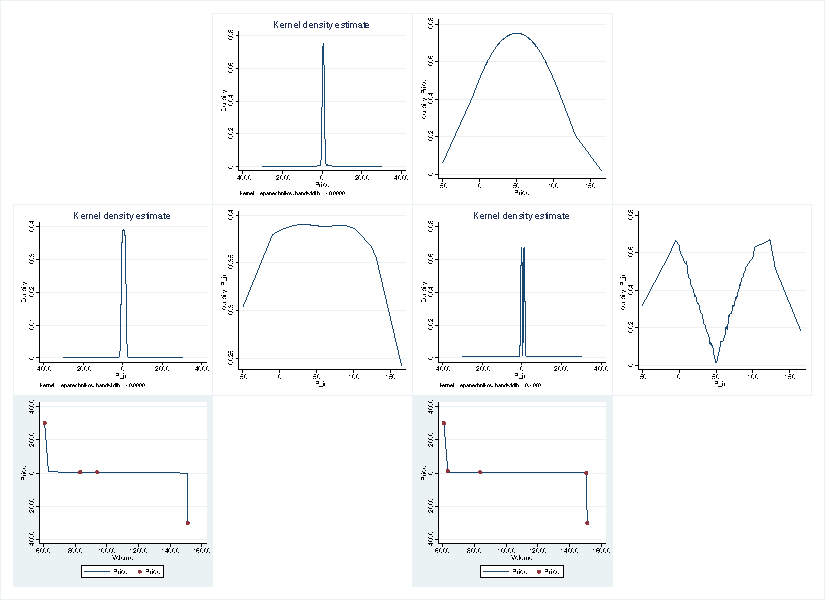
\includegraphics[trim=0.2cm 0.25cm 0.2cm 0.2cm, clip=true, height=90mm]{figch2/comparison1.pdf} 
\caption{Comparison of bandwidths: Large bandwidth in first stage}
\label{bandwidthcomp1}
\end{center}
\emph{Note: Large bandwidth in first stage (top row), large bandwidth in second stage (second row left), small bandwidth in second stage (second row right), Resulting selection of points for large bandwidth in stage one and two (bottow row left, A) and selection of points for large bandwidth in stage one and small bandwidth in stage two (bottom row right, B).}
\end{figure}


\begin{figure}[!ht]
\begin{center}
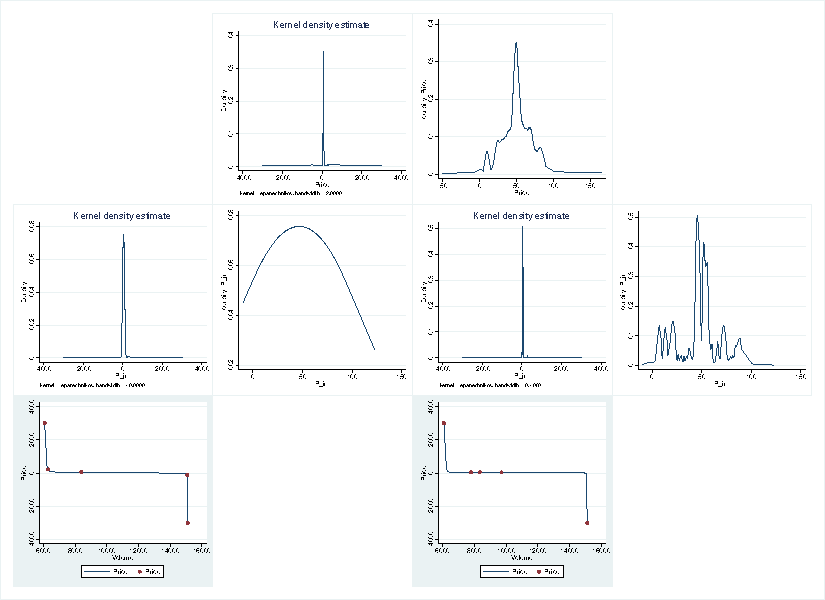
\includegraphics[height=90mm]{figch2/comparison2.pdf} 
\caption{Comparison of bandwidths: Small bandwidth in first stage}
\label{bandwidthcomp2}
\end{center}
\emph{Note: Small bandwidth in first stage (top row), large bandwidth in second stage (second row left), small bandwidth in second stage (second row right), Resulting selection of points for large bandwidth in stage one and small bandwidth in stage two (bottom row left, C) and selection of points for small bandwidth in stage one and two (bottow row right, D).}
\end{figure}


In these graphs, the top row shows the first stage KDE, over the whole function on the left and zoomed on the right. The large bandwidth in figure \ref{bandwidthcomp1} shows the impact of smoothing on the estimates of the first derivative as compared to figure \ref{bandwidthcomp2}.
The second row in both graphs shows the second stage KDE in two versions: Using a wide kernel bandwidth on the left and a tight bandwidth on the right. Again, we disclose the result as seen over the whole function (left) and zoomed on the central price range (right).\\

The third row details the original demand function with the final point selection given the bandwidth selection as given by the two rows above. 
Regardless of the first stage bandwidth, we see that a large bandwidth in the second stage KDE easily distorts the point selection. Selected points of type $k=2,4$ are either two centred or too wide as a result of the second derivatives being smoothed excessively and not precisely representing the local specificities of the curve. \\

The right hand side of both figures show that a tighter bandwidth on the KDE can easily mistake large slope changes due to steps in the bid functions as the appropriate points of maximum curvature of the full bid function and thereby make an error. Therefore, we apply a sensitive second stage KDE on rather smooth estimates of the first derivatives, which yields an adequate point selection in our setting (figure \ref{bandwidthcomp1}B). \\

The bandwidth selection received much attention in this work in order to obtain a reasonable selection of points based on local information of the curves, while achieving a satisfying robustness to noise in the bid function. We are aware that this subjective setting of the bandwidth is not without consequence for our work. However for computational reasons\footnote{The point selection algorithm ran for more than two weeks in the current setting.}, we do not run a full robustness test on this choice ex-post.

\subsection{Outlier detection and removal}
\label{outlier}
In some rare cases, our point selection mechanism does not work. This is the case when curves have very small number of points at a kink and it is thus very difficult to detect their curvature. \\

As a result, the selected points are then quasi in-differentiable from the next selected point type, i.e. a point of type $k=2$ is almost identical to the selected point $k=3$. The code is unable to select the right points due to a data lack on the original curve (second derivative on a constant slope up to POI is zero).\\

We screen for adjacent points that display quasi no variation in volumes. Figure \ref{diff37rangehist} shows a histogram of volumes differences over 2 selected points (from $k=2$ to $k=4$) and reveals a positive mass point at zero, indicating outliers that do not display any volume variation between points of the same bid function. We use the histogram to identify and drop those outliers from our dataset. 

\begin{figure}[!ht]
\begin{center}
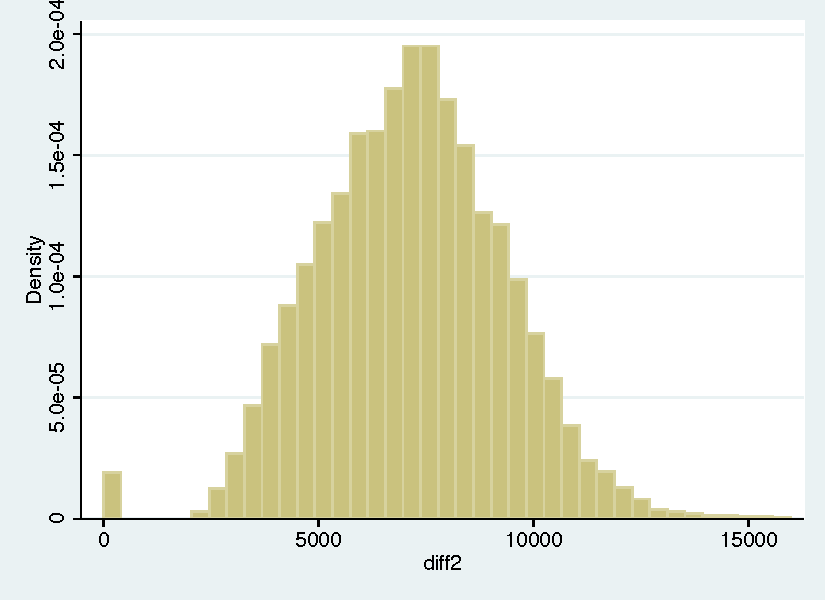
\includegraphics[height=50mm]{figch2/diff37rangehist.pdf} 
\caption{Histogram of volume variation between points}
\label{diff37rangehist}
\end{center}
\emph{Note: The histogram shows the volume difference between points $k=2$ and $k=4$ of the same bid functions. }
\end{figure}

\end{subappendices}













%\renewcommand{\tabularxcolumn}[1]{m{#1}}
%\newcolumntype{Y}{>{\centering\arraybackslash}X}
%\newcolumntype{R}{>{\flushright\arraybackslash}X}


\renewcommand{\thesection}{\arabic{chapter}.\arabic{section}}


\chapter{Investigating the Impact of Uncertainty on Firms with Dynamic Costs : A Case Study of the French Electricity Market}
\label{chap:ch2}
\cleardoublepage

\doublespacing
In the last chapter, we have given some attention to a methodology that allows us to use functional data for reduced form analysis. In this chapter, we focus on the economic questions that can be asked using such a methodology. Specifically, we focus on an investigation of the effect of uncertainty on the behavior of electricity producers, and testing the predictions of our first chapter, by leveraging the results of our second chapter that allow us to compare schedules to one another. \\

There exists a consensus that dynamic costs, also referred to as ramping or adjustment costs, are important on the electricity market\footnote{ \cite{anderson2005supply},  \cite{hobbs2001next}, \cite{hortacsu2008understanding}, \cite{reguant2011welfare}, \cite{sewalt2003negative}. }. These are the costs incurred by a producer when production varies. 
The importance of uncertainty for the expectation of dynamic costs is shown in chapter 1. Uncertainty itself on the electricity market as well as estimates for the value of ramping costs have been studied empirically by \cite{wolak2007quantifying}, in the case of step functions. %, who specifies and captures in a single index the uncertainty that suppliers face on the electricity market. %: (i) the uncertainty from not knowing the aggregate supply function served by all other suppliers and (ii) the uncertainty about the realisation of the market demand. , who specifies and captures in a single index the uncertainty that suppliers face on the electricity market.   
We focus on two sources of uncertainty for traditional electricity suppliers, namely uncertainty about the realization of the market demand and uncertainty from the inherently unpredictable meteorological situation
%forecasts 
(which affects renewables generation). 
We propose a methodology to measure this uncertainty and its impact on firm strategies on the electricity market. %due to the existence of dynamic costs. %Our methodology allows to address policy questions of high relevance, such as the optimal spatial distribution of renewable production facilities. \\

Electricity as a market is very important in and of itself ($\$2$ trillion in worldwide sales in 2010). It is also a crucial input for many industries; power outages induce very large costs to society (\cite{lacommare2004understanding}, \cite{reichl2013power}). 
%The importance of electricity for modern economies is undeniable. Indicators of its importance are the size of its market ($\$2$ trillion in worldwide sales in 2010) and the fact that electricity is an input for many other industries. 
%Market failures, which arise in the form of mis-pricings or network breakdowns, have very large economic costs to society and deserve more attention. 
%The analysis of its markets is highly interesting from an economic perspective. 
The electricity market is, however, quite different from the markets for other commodities in a few respects. First, electricity cannot be efficiently stored. As a consequence, electricity markets are high frequency (prices can update down to 15-min intervals) and firm strategies are purer as they are free of stock management considerations. \\

Second and in addition to non-storability, a generation surplus cannot be disposed of freely\footnote{The common assumption of free disposal as made in standard microeconomics is violated.}. Thus, generation of electricity must always be matched with consumption in real time (modulo a small tolerance). This represents a hard constraint on the market\footnote{Mismatches between consumption and generation ultimately result in power outages.} and forces suppliers to be reactive. However, this reactivity is costly as plant operators incur dynamic costs when adjusting production and the larger the adjustment made, the larger the cost. 
Hence, suppliers face a trade-off between cheap generation of electricity and costly reactivity to the demand realization. Indeed, no single generation technology exists that satisfies both cheap generation and sufficient reactivity to allow production fluctuations at a reasonable price . Existing generation techniques are either cheap and unresponsive, e.g. nuclear plants, or expensive and flexible, e.g. gas turbines. \\
 
Interestingly, we also observe negative prices. In France for example, during the weekend of the 15$^\text{th}$ June 2013, the price per MWh dropped to $-200$\EUR{}. This contrasts to the yearly average of approx. $ 45$\EUR{}/MWh and is generally understood as a sign that subsidizing consumption temporarily is cheaper for a supplier than shutting down a plant \cite{epexwebsite1}\footnote{``Negative prices are a price signal on the power wholesale market that occurs when a high inflexible power generation meets low demand. Inflexible power sources can’t be shut down and restarted in a quick and cost-efficient manner. Renewables do count in, as they are dependent from external factors (wind, sun)."}.  The increase of the share of renewable generation in the energy mix contributes to the occurrence of negative prices on the market. 
% Renewables generation benefits from a feed-in guarantee on the electricity grid. 
The intermittency of renewables causes large residual demand shocks \cite{epexwebsite1}. The unreliability of renewable generation also means that more flexible plants (i.e. plants with lower dynamic costs) are required to provide rapid responses to fluctuations in production from renewables \cite{ren2013renewables}. \\

Furthermore, uncertainty arises from the fact that renewable production is a local and dispersed production, but feeds into a national market with a single price. When meteorological conditions change, the geographic production profile also changes. This further complicates the predictability of renewables generation and contributes to the uncertainty that electricity producers face when playing %bidding 
on the electricity %EPEX Spot 
market \cite{meibom2009operational}.\\

This paper explores the effect that the absolute level of uncertainty about residual demand has on players' strategies on the electricity market. In the light of the existence of dynamic costs, which are inherent to the production technologies, uncertainty is costly to suppliers as shown in chapter 1. Thus when faced with uncertainty, we expect that electricity producers smooth production volume over time in order to minimize dynamic costs. In a single market interaction with a symmetric oligopoly and linear demand functions this translates to playing a steeper supply function when uncertainty is high. The detailed intuition behind the predictions tested is given in section \ref{intropredict}. 

\label{introresults}
We show that uncertainty does impact supplier strategies. However, this prediction and result only apply locally to the central, flat and linear part of the supply bid function. Towards the high and low volume extremities of the bid functions when capacity constraints start to matter, bid functions qre stepper and the effect of uncertainty vanishes. Furthermore, we observe results that indicate that demand-side bidding is also impacted by uncertainty.  \\
%However the prediction tested is only partially validated by the data, in that only part of the curves are indeed getting steeper as uncertainty increases whereas others get less steep. We discuss how and why those discrepancies might arise at the end of the paper.  

%In the light of the existence of dynamic costs, which are inherent to the production technologies,  uncertainty is costly to suppliers \cite{bergesmartimort2014}. 
%The industry set-up allows suppliers to trade the uncertainty on three different markets that differ the lead time up to delivery *** OR 
%The converse holds: acquisition of information about expected residual demand is valuable. 
%The industry set-up allows the incorporation of new information about expected demand by its segmentation into three markets that differ by the lead time up to delivery: 
%a longterm bilateral contracting market, a one-day ahead market and an intraday balancing market for last-minute adjustments. 

We focus on the French one-day ahead market, EPEX Spot. This market is a divisible goods auction and 
particularly suited for our analysis as we observe data on the full aggregate bid functions for both supply and demand.  We introduce the market's auction format and rules in section \ref{epexall}.\\
%***** WE CHOOSE MARKET BECAUSE OF DATA AVAILABILITY NOT BECAUSE OF SPECIFIC PLACE IN INDUSTRY -> CAUSALITY NOT 
%we explore the link between uncertainty and dynamic costs. Theoretical models imply that uncertainty about the market outcome impact player's strategies on the market \cite{bergesmartimort2014}. More specifically, this paper aims to better understand the shape of aggregate bid functions on the EPEX Spot market and tests the impact of the absolute level of uncertainty  on the submitted bid functions of suppliers. In the presence of dynamic costs, we expect that electricity producers smooth production volume over time in order to minimise these dynamic costs. In a single auction this translates to bidding a steeper supply function when uncertainty is high. The detailed intuition behind the predictions tested is given in section \ref{intropredict}. 
The dataset and its sources are presented in section~\ref{datasection}.
We develop our identification methodology in section \ref{newapproach}. Our empirical strategy relies on the non-parametric, comparable point selection technique presented in chapter \ref{pschapter}. 
We reuse the selected points of the previous chapter for our analysis here. 
We present and interpret the results in section \ref{resultsplusinterpret}. 
%In section XXX, we focus on welfare analyses.**** TO DO : We first apply the model to quantify the effect of uncertainty in terms of price differentials on the market and then address the social cost, which could be avoided if geographic plant location was not decided on by individual investors, but by a social planner, who minimised uncertainty of renewables production. 
Finally, we discuss some overarching points in section \ref{discussgeneral} and conclude in section~\ref{conclusion}.


\subsection{Literature review and contribution}
\label{litrev}

There exists a literature on supply function equilibria initiated by \cite{KM}. 
In traditional models, firms choose between quantities (Cournot) or prices (Bertrand) as their strategic quantities. In the intermediate case, firms choose a relationship between quantities and prices, namely a supply function. This is the focus of the supply function equilibrium models.
%In this literature, firms do not have to choose between prices or quantities as a strategic variable, but submit a supply function which matches the quantity supplied by the firm to the price of the market. %, which endogenously determined by the aggregate supply and demand. 
A key ingredient of these models is uncertainty.\\

Supply function equilibrium models are very relevant for the analysis of electricity markets, since many electricity market designs allow firms to submit a price-volume function rather than a specific price or quantity. \cite{Newgreen}, \cite{newbery1998competition} and \cite{bolle1992supply} have used these models to analyze competition on the electricity markets. \\

These papers have contributed to a broader investigation of the competition on the electricity markets, which has also been looked at from empirical perspectives \cite{wolfram1998strategic, borensteinetal2002marketineffs}.
While those initial papers have focused on the supply function equilibria of the market, they have abstracted from some technological specificities for the sake for simplification. \\

One such aspect that we are interested in and that has been the subject of research in recent years is the importance of dynamic costs for electricity production. \\
% First paper:
Our first chapter extends \cite{KM} to derive predictions on firms facing dynamic costs in a supply function oligopoly under uncertainty. 
When varying production is costly, suppliers take these costs into consideration by submitting steeper functions when facing more uncertainty, in order to limit the range of variation in production.
\cite{reguant2011welfare} develops a model and an empirical strategy to measure dynamic costs on the Spanish one-day-ahead electricity market. She finds that ``complex bids", which allow firms to minimize dynamic costs by linking production in one time period to production in a subsequent time period, reduce the volatility and the level of prices on the market.  Her work is also unique in terms of data availability. By using individual bid functions she is able to produce estimates of start-up and ramping costs per production technology. \\

In order to quantify dynamic costs on the Australian electricity market, \cite{wolak2007quantifying} derives a methodology to recover estimates of the parameters of parametric cost functions at the level of the production unit. His identification is based on the assumption that each profit maximizing supplier knows the distribution of shocks on the demand function when playing on the market. Uncertainty is thus an explicit ingredient of his paper and he captures two sources of uncertainty in a single index: (i) the uncertainty from not knowing the aggregate supply function served by all other suppliers and (ii) the uncertainty about the realisation of the market demand.  The recovered cost functions quantify the cost of varying output. Forward contracts are useful to avoid output variations. By comparing the observed  level of forward contracting (assumed to be the profit maximizing choice for production variation) with the theoretical minimum cost production pattern, he %cannot reject the hypothesis that ramping costs are important for suppliers. 
does not find support for ramping costs.\\

We contribute to this literature by providing an empirical analysis of the French electricity market.
Specifically, we look at the impact of uncertainty on supplier strategies and take this as evidence that dynamic costs matter. 
 Our approach to separate out the uncertainty from market demand expectations and predictability of renewables generation is novel. Both proxies for uncertainty used are new, uncertainty from market demand is inferred from the prediction errors that firms make in a demand estimation and uncertainty from renewable production is computed in a bottom-up approach from local weather forecasts.
Instead of opting for a time series regression, we understand all hourly auctions as a cross-sectional dataset and control for the time of the day by using continuous transition variables for daytime periods. Similarly, we control for seasonality using continuous variables rather than dummies.  Thereby, %we circumvent the problem of dummies in our regressions, which are black boxes for the interpretation.
we are able to leverage our dataset and increase the sample size for each of our regressions and improve the precision of our estimates. \\


%maybe 4. (authors of Operational costs induced by fluctuating wind power production in Germany and Scandinavia) give the link from production intermittency of renewables to operational costs for the market. In particular, they separate out the operational costs due to predictatbility and variability of renewables generatio. 

%
%\subsection{Larger research question - link to electricity storage and demand response policies}
%This paper feeds into a larger research project on how a government should allocate resources between developing renewable's generation and alternative policies, such as incentivising research on electricity storage or the pushing of demand response policies. 
%
%Electricity storage refers to techniques to defer consumption of electricity to a later point in time\footnote{** Say example, say problems: Power-to-gas, too expensive on large scale}. 
%Demand response measures allow to reduce electricity consumption at peak times, e.g. by deferring or deleting consumption on the grid\footnote{** say example and problems, "effacement energetique, pas repandu en europe, existe aux US, probleme contraignant.}. 

Furthermore, our work contributes to the empirical literature testing strategic behaviour of market participants. 
 Generally, these studies focus on point-wise analyses for reasons of data availability. Not only does this cause endogeneity problems when the data used is equilibrium data, but also the analysis is restricted to an understanding of the usually observed outcomes of the market. \\
 
In our setting, we benefit from an interesting dataset in which we observe full aggregate bid functions of players. The functions describe the players' behaviour both in the region where the equilibrium is likely to occur as well as in regions that  rarely have an impact on the equilibrium outcome. As such, they provide a much fuller description of the firms' strategies. 
The additional information contained in the full aggregate bid functions has been used extensively in theoretical work (notably in the supply function equilibria literature mentioned above). 
However, few papers exploit these full bid functions empirically. \\
%
%This work is also related to another strand of the literature concerned with the functional analysis of data in an economic context. From a theoretical perspective, we many theoretical papers have derived predictions on the supply or demand functions\footnote{CITE SOME LINEAR EXAMPLES.}. However, often subject to strong simplifications such as using linear functions. In the domain of non-linear functions, we observe the work by SOME EXAMPLES. 
%
%From an empirical perspective, functional analyses remain the exception, arguably for reasons of data availability.
For the government bond market, \cite{pw2002etude} and \cite{ozcan2004logistic} use a parametric approach to this functional data for a description of the variation of bid functions with respect to exogenous factors and an investigation of the revenue superiority of the uniform or discriminatory multi-unit auction mechanism, respectively. On the electricity market,  \cite{wolfram1999measuring} leaves the analysis of equilibrium data to investigate duopoly power of firms on the UK day-ahead spot market. Instead, she uses information from the whole aggregate supply function to investigate the impact of price caps for electricity producers. Using an analysis conditioned on 25 different demand levels, she shows that the introduction of price caps resulted in a counter-clockwise rotation of the aggregate supply function. She relates these results to produce a lower bound on the extent to which firms can increase their prices above marginal costs when regulatory pressure makes it advantageous to do so. Thereby, she contributes  empirical evidence for the distorting effects of price caps. \\

Our work adds to this empirical literature using the information contained in the full bid functions 
by developing a non-parametric approach which allows to condition our analyses on multiple, representative points of the bid functions. The statistical ingredients rely on \cite{ramsaysilverman2005functional} and are detailed in chapter \ref{pschapter}.
Thereby we are able to leverage our dataset, increase the sample size in individual regressions as well as obtain a fuller picture of the effects of exogenous variables on the behaviour of electricity producing firms. We emphasize that out approach allows to overcome structural restrictions underlying previous parametric approaches, e.g. the symmetry of the logistic function used in \cite{pw2002etude}.

%this literature by  on functional analyses, specifically to that on the electricity market. By conditioning our analysis on different points of the market bid functions, we are able to investigate non-linear effects of exogenous factors on the shape of the bid functions.  While functional analysis have been used in the past, our non-parametric, point-specific approach is novel in the economics literature. Our approach  


\subsection{Theoretical prediction}
\label{intropredict}

%%%%%%%%%%%%%%%%%%%%%%%%%%%%%%%%%%%%%%%%
%%%%%%%%%%%%%%%%%%%%%%%%%%%%%%%%%%%%%%%%
%*** ADD OBJ FUNCTIONS AND QUick DERIVATION TO SUPPORT INTUITION
%%%%%%%%%%%%%%%%%%%%%%%%%%%%%%%%%%%%%%%%
%%%%%%%%%%%%%%%%%%%%%%%%%%%%%%%%%%%%%%%%

We test the impact of uncertainty of supplier strategies by testing the prediction that suppliers bid steeper supply bid functions when faced with a larger uncertainty concerning the outcome of the (residual) demand realisation.\\
%More specifically, in this paper we aim to better understand the shape of aggregate bid functions on the EPEX Spot market and test the impact of the absolute level of uncertainty on the suppliers submitted bid functions. 

In a discontinuous setting, where the supplier produces volume $Q_H$ of electricity in hour $H$, we assume that he faces a cost function $C_i(.)$ for each production plant $i$. This cost function depends on both marginal costs of production as well as the dynamic costs for changing production rapidly: $C_i \bigl( (Q_H), (Q_H - Q_{H-1})^2 \bigr)$. The larger the variation in production between hours, the larger the dynamic costs. 
Even when the expected residual demand is constant, there are still fluctuations in the production due to possible shocks to the residual demand. The larger the shocks, the larger the change in production and thus the larger the dynamic costs. 
%Given a constant expected residual demand, unpredictable shocks on the demand function induce these dynamic costs. 
Consequently, increased uncertainty (as represented by shocks on the demand function) translates into increased expected dynamic costs. We assume that the profit maximizing supplier knows the distribution of shocks on the demand function when choosing his supply function.  In order to minimize these costs, the producer can choose a steeper supply function when uncertainty is high. We want to test this prediction. \\

%The intuition behind the predictions tested in this paper is illustrated in figure \ref{predictslope} using a stylised case. 
We illustrate the intuition behind this prediction using a stylised case in figure \ref{predictslope}. The graphs depict a situation in which a single, risk-neutral supplier bids a supply function to supply electricity in the hours 9 and 10 of the next day. For both hours, the supplier faces a constant expected residual demand function represented by $E(D)$. In a static optimisation problem, the supplier would bid a supply function $S_0$ in both auctions. \\

\begin{figure}[!ht]
\begin{center} \makebox[\textwidth]{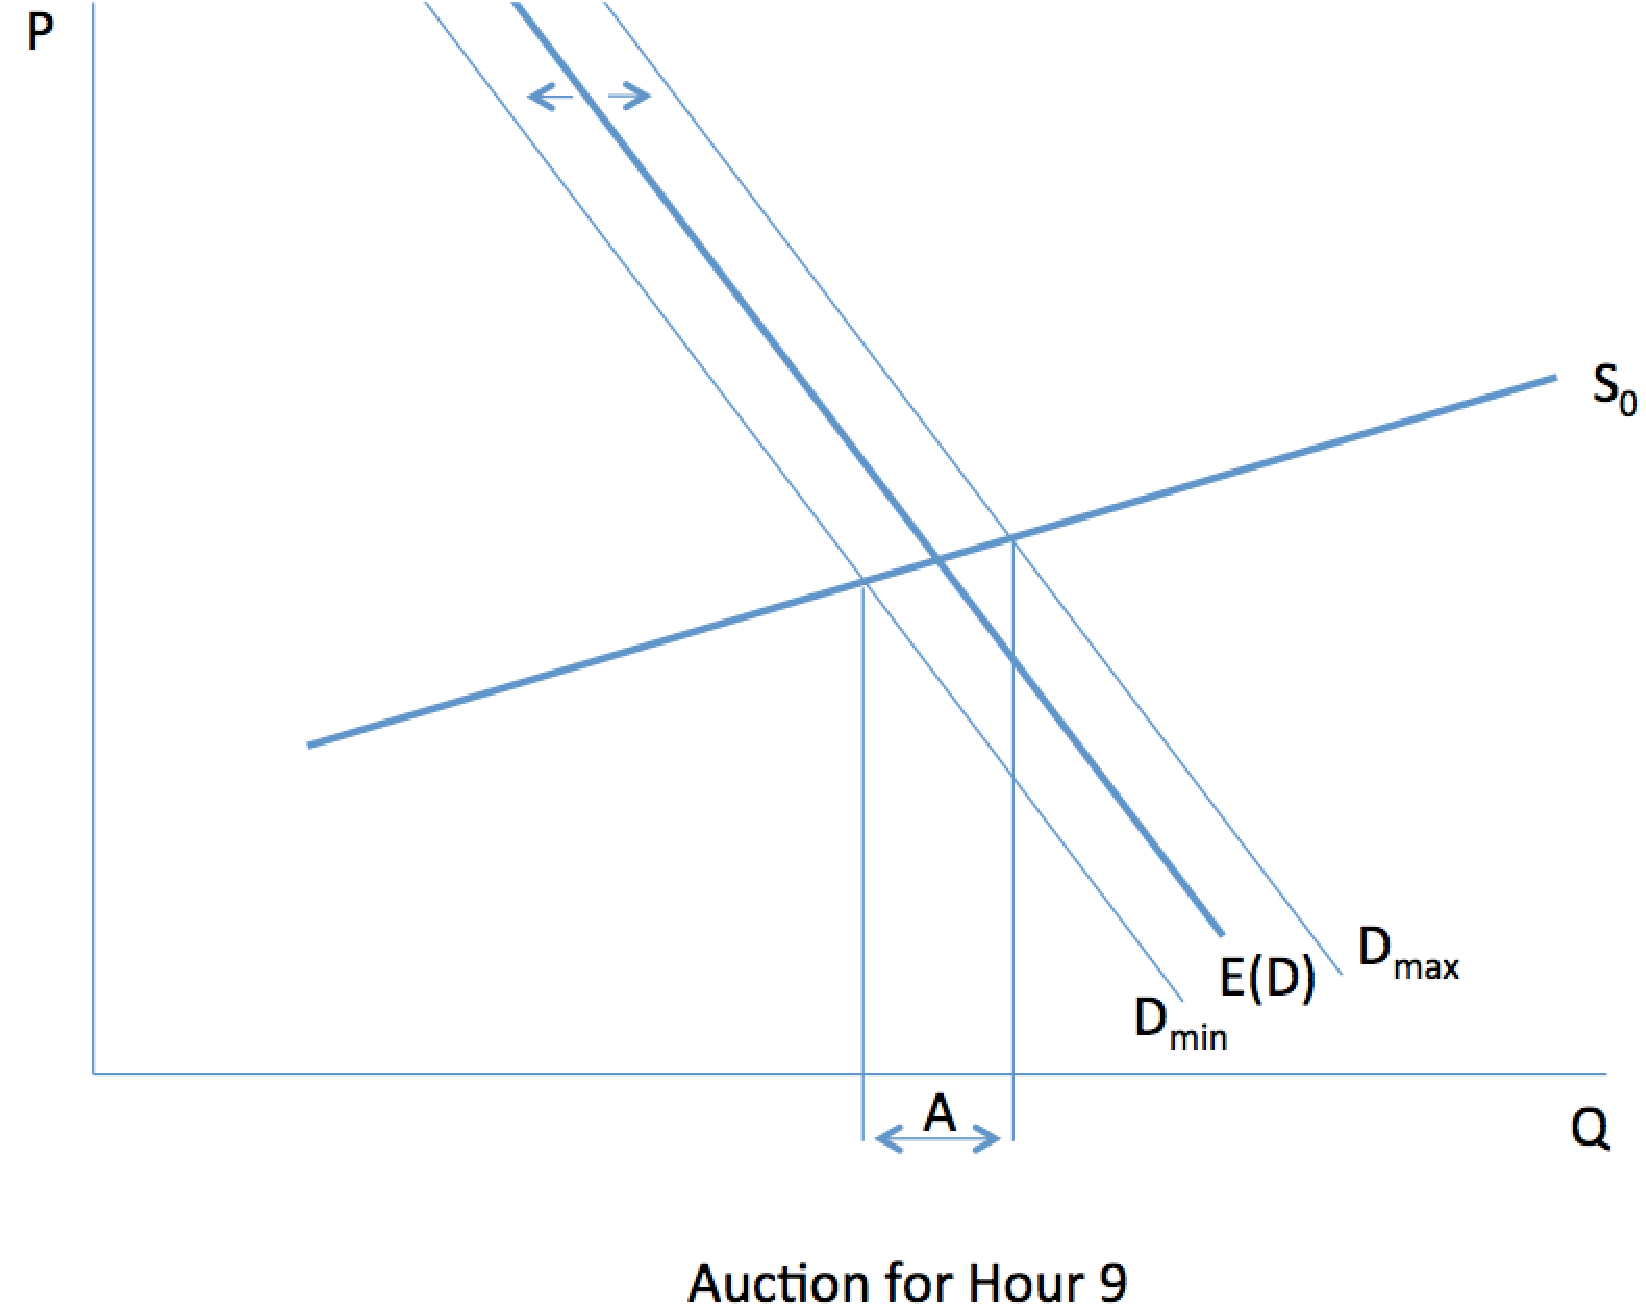
\includegraphics[height=50mm]{figch2/Shot35.pdf} \hspace{0.03cm} 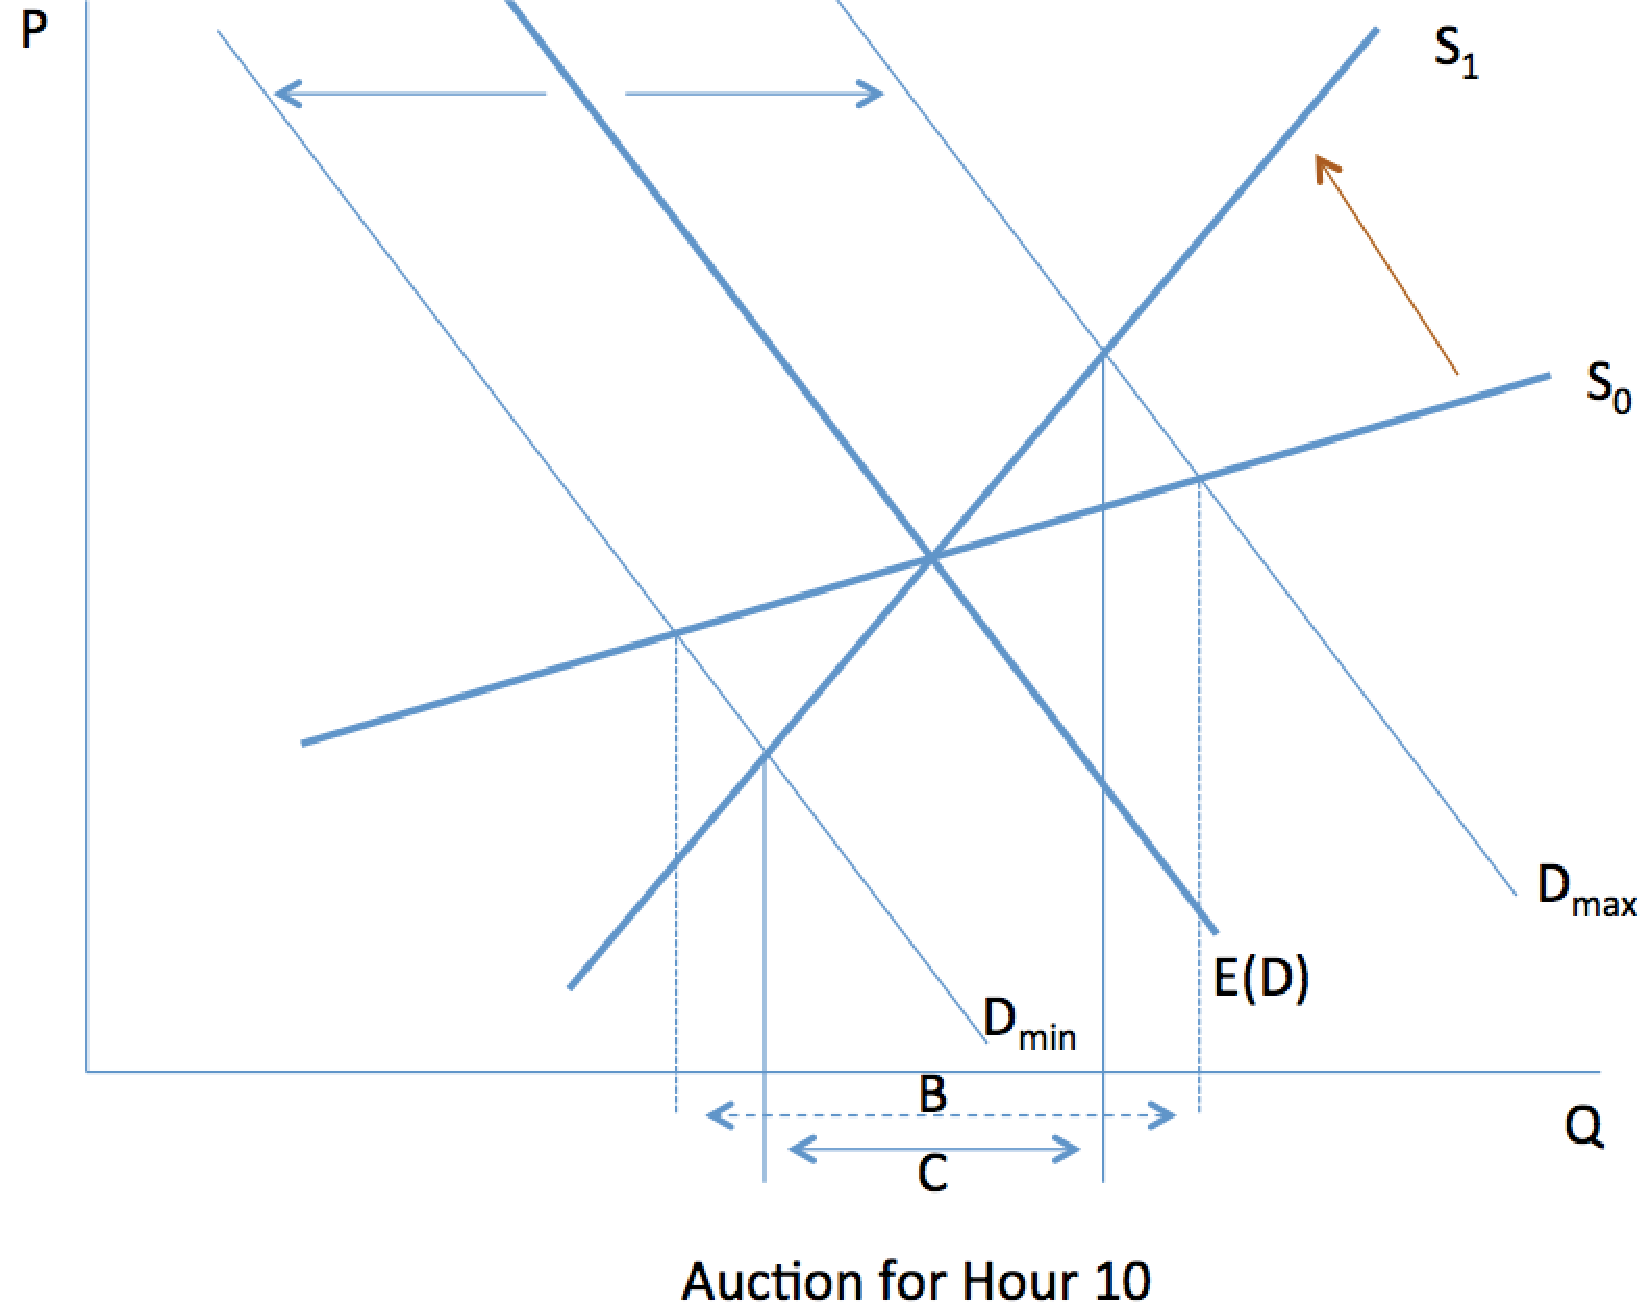
\includegraphics[height=50mm]{figch2/Shot36.pdf} %\hspace{0.03cm} \includegraphics[height=50mm]{predictslope11.pdf}
} \end{center}
\caption{Illustrating the effect of increased uncertainty.}
\label{predictslope}
%{\small Note: }
\end{figure}

The uncertainty in the market is represented %in the model (to move away from model for intuition
 by the width of the envelope of shocks that affect the residual demand function (represented by the arrows on $E(D)$). Thus, in each hour, the residual demand fluctuates between $D_{min}$ and $D_{max}$, where the range between the extremal demands may vary from one hour to the next. \\
 
Before submitting a supply function to the market, the supplier estimates the distribution of probabilities of demand shocks that he will face.  %The price elasticity of the supply function is given by the slope of the supply function. 
In hour 9, the supplier is able to rather precisely predict the realisation of the demand function in the auction, i.e. it realises within a tight confidence interval. In hour 10, however, uncertainty in predicting the outcome of the demand realisation has grown strongly as represented by the much wider confidence interval on the demand realisation. \\

Given a fixed supply bid function $S_0$, the possible range of quantities to be produced by the supplier when going from hour 9 to hour 10 has increased due to the increase in the size of the uncertainty (interval on the Q-axis has grown from length $A$ for hour 9 to the dotted length $B$ in hour 10).\\

Now, we assume that the supplier faces dynamic costs, i.e. it is costly for production to vary on top of any traditional marginal cost consideration and the larger the variation, the larger the cost.  Then in the case of a fixed supply bid function ($S_0$ in both auctions), an increase in uncertainty implies an increase in expected dynamic costs. \\

The supplier's reaction to increased uncertainty is therefore to bid a steeper supply function $S_1$ in order to trade-off static optimality and dynamic effects. As a consequence, the range of volumes produced in equilibrium is reduced (the firm produces in the range $C$ instead of $B$). When seen over time, these considerations lead to a smoother production as compared to a constant supply curve: demand shocks are absorbed through a higher price volatility and a lower production volatility. \\%In other words, by introducing dynamic cost considerations, volatility in prices has become comparatively cheaper than volatility in production. 


If cautious behavior under high uncertainty is true for all firms on the market and each firm has the same expectation of the probability distribution of the uncertainty, then the reaction of bidding a more price inelastic supply function to increased uncertainty should be observable on the aggregated supply function. \\

We emphasize that this prediction relies on linear demand and supply functions and does not incorporate capacity constraint considerations (both upper and lower bounds on the production volume of plants), which are also important on the market.  Furthermore, we have outlined our prediction using a discrete time-setting. 
The continuous version of this analysis on dynamic costs is explored in detail in chapter 1.\\ 
%Finally, we consider that the number of bidders stays constant across auctions. Holmberg 2004 shows that the slope of the unique symmetric equilibrium supply function falls with the number of 
% The full blown model solves the problem in the case of a symetric oligopoly of suppliers facing uncertain demand and subject to dynamic costs of production. The essence of the model is for a supplier $i$ to maximise its expected profit: 
%
%\begin{equation}
%\displaystyle{\max_{S_i(p)}}~\mathbb{E}\left[\int_{0}^{T} \left(p(\theta(t))S_i(p(\theta(t))) -C\left(S_i(p(\theta(t))),\frac{dS_i(p(\theta(t)))}{dt} \right)\right)dt\right]
%\end{equation} 
%
%with $S_i(p)$ the supply schedule as a function of the price $p$, $f(\theta)$ the distribution of demand shocks $\theta$, $C(\cdot)$ the cost function depending on the level of production and its variation, $t$ the time, and $T$ the time period over which the flow of profits is maximised. This formula is only presented to give the gist of what is done, the formal maximisation program is different\footnote{This comes from the fact that one of the difficulties lies in the representation of the dynamic costs: the key ingredient in such a model is uncertainty, however, the most natural way to represent dynamic costs is by taking the time derivative of the production. Taking the derivative of a stochastic process is not possible, which is why the program has to be written in a different way. This is a technicality that is developed in much detail in the paper.}.   
%
%This model is solved analytically in the case of linear demand functions and symmetric oligopoly. The main result is that supply functions are linear too, and that their slope evolves with the time derivative of the amount of demand uncertainty. This effect is mainly driven by the use of a time continuous model, which allows to derive analytical results, but which implies myopic solutions: only local dynamic effects (the time derivative of the amount of demand uncertainty) can be derived. The authors believe that this result is a consequence of the continuous formulation of the model, we therefore focus empirically on the impact of the level of uncertainty on the strategies of the suppliers.

The present paper tests this mechanism empirically and understands an increase in the slope of aggregate supply bid functions due to an increased level of uncertainty as evidence that firms minimize dynamic costs across auctions. %\footnote{In a companion paper ***REF, the authors explore the effect of the dynamics of the uncertainty, as opposed to the level of uncertainty investigated in this paper, on the bidding behaviour of electricity supplying firms.}.


%
%This narrative allows for two distinct mathematical interpretations. On the one hand, the absolute level of uncertainty could account for steeper supply schedules. On the other hand, one could think that it is the variation in uncertainty, and not uncertainty itself, that drives the dynamic bidding behaviour. 
%
%The first interpretation is straightforward from the previous paragraphs. The second one comes from a more detailed analysis of the dynamics of demand shocks. More precisely, when modelling shocks it is possible to obtain a situation where the level itself of uncertainty is not the driving force but the variation of the uncertainty is. This distinction can arise when a the level of demand is close to its expected maximum or minimum value. Close to the boundaries, it is expected to stay there longer than if it is close to its expected value. One can think of this as a producer forming his anticipation of demand based on different demand scenarios. 
%
%There can be many different situations leading to an average demand, but for demand to be close to its maximum or minimum anticipated value, a lot of events must realise in a specific way. Therefore, when close to a boundary, there is not much uncertainty as to which scenario lead to such a situation, whereas multiple scenarios can lead to an average demand value. The level effects of uncertainty, i.e. when close to a boundary there is less potential variation in demand than when close to its expected value, may cancel out, leaving the dynamics of the uncertainty as the only driver for bid shifting of suppliers : when uncertainty increases these effects become unbalanced and optimal bids change.


%These effects, i.e when close to a boundary there is less potential variation in demand than when close to its expected value, can balance out and leave only a pure dynamic effect, that is that the variation in uncertainty drives the dynamics of the optimal bid submitted by producers: when uncertainty increases these effects become unbalanced and optimal bids change. 
%
%Berg\`es and Martimort (in prep) develop a full mathematical analysis of the dynamics of supply function equilibria under uncertainty when production is subject to dynamic costs, which points towards the possibility for the second more involved and less intuitive effect to exist. This paper tests empirically both mechanisms and understands an increase in the slope of aggregate supply bid functions due to increased uncertainty as evidence that firms minimise dynamic costs across auctions.

%If there is low uncertainty on both low and high frequency volatility over time, the supplier can reasonably well anticipate the dynamic costs between production volumes. If now there is high uncertainty on high frequency volatility (noise) and low uncertainty on the trend, it means that the specific trajectory of demand is quite uncertain but it might not change much statistically speaking from a well anticipated trajectory. On the contrary, what can be quite informative is the variation in uncertainty. If the uncertainty increases sharply, it means that we know that there might be large shocks to the demand, which is not the same as having a low amount of information about an otherwise typical demand trajectory during the day. 

%In other words, constant high uncertainty can point towards daily shocks, i.e. the anticipation of the heating required for the day was off for every hour by the same amount, whereas varying uncertainty can point towards knowledge of local shocks than can lead to high dynamic costs. This is why variation in uncertainty could be the actual driving force behind changes in supply curves from hour to hour. The paper by \cite{bergesmartimort2014} predicts the latter relationship. This paper tests empirically both mechanisms and understands an increase in the slope of aggregate supply bid functions due to increased uncertainty as evidence that firms minimise dynamic costs across auctions.

%
%*********
%
%Alternative idea of explanation: 
%
%Costly variation in the predictability of demand shock is due to to coordination failures in the market. When uncertainty increases sharply, many firms in the industry aim to adjust their bidding behaviour. Expectation differences (does not work with symmetric players) lead to exacerbation of natural uncertainty and thus increase dynamic costs. 
%Private information in bidding distorts the adjustment bidding behaviour of firms and can exacerbate over/undershooting of aggregate bid expectation when adjusting to new uncertainty environment. 
%
%*********



\section{The EPEX spot market}
\label{epexall}
\subsection{General background}
\label{epexbackground}
The EPEX Spot market is an auction market, which allows firms to trade electricity 12-36h ahead of delivery. It covers France, Germany with Austria and Switzerland. The volume traded on Epex Spot represents $12\%$, $40\%$ and $30\%$ of the total electricity consumption in these countries respectively in 2013 \cite{epexwebsite1}.\\

The EPEX Spot market has considerably gained in importance over time and the daily trading volume has almost quadrupled since $2005$, whereas the total electricity consumption has essentially remained constant. The graph in figure \ref{volconsfr} shows these trends very clearly. Furthermore, it shows the significant volatility of the market trading volume (as indicated by the width 
%\footnote{Figure \ref{rollsdvolconsfr} in the appendix shows the evolution of the standard error on which the confidence interval in figure \ref{volconsfr} is based.} 
of the grey-shaded confidence interval).  \\
\begin{figure}[!ht]
\begin{center} \makebox[\textwidth]{
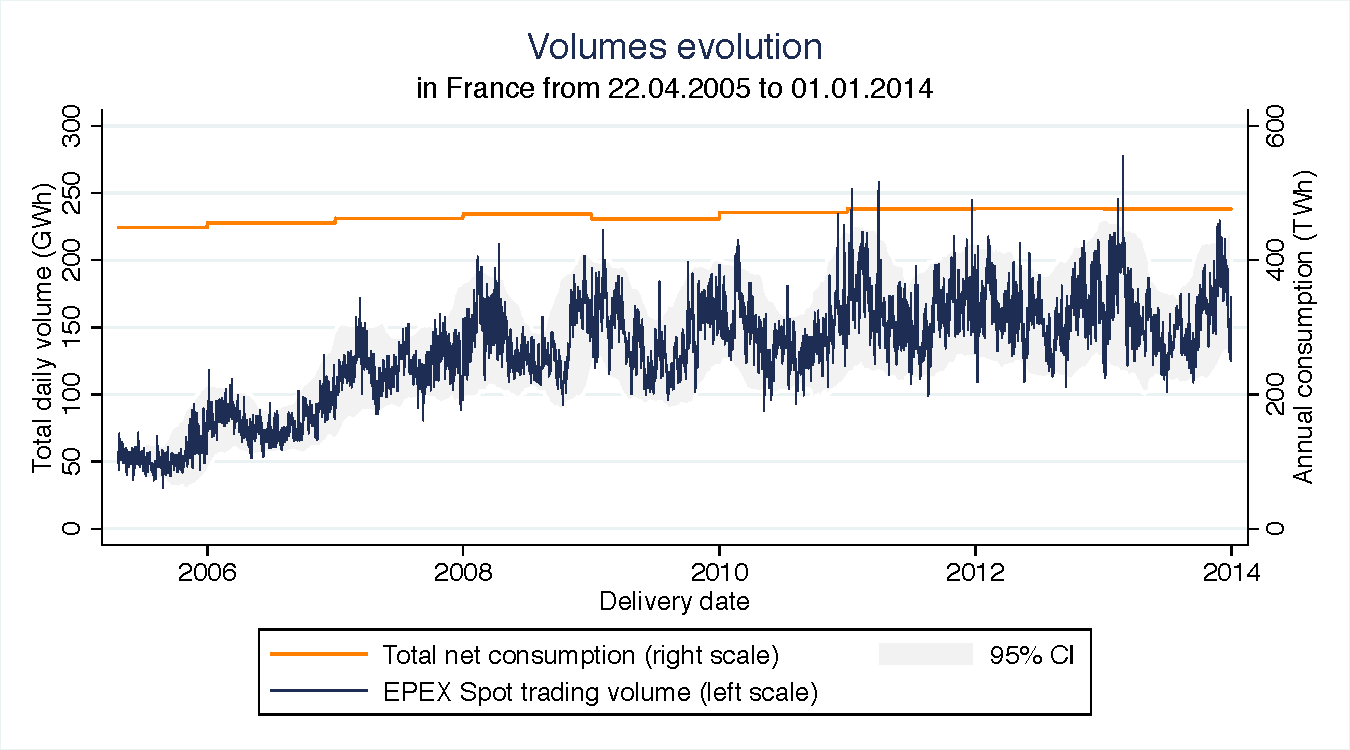
\includegraphics[height=74mm]{figch2/volplusconso3.pdf} 
} \end{center}
\caption{Traded volume plotted against total annual consumption}
\label{volconsfr}
% graph updated on 24.11.2014
{\small Note: Total consumption is netted of the electricity withdrawal at the level of the production unit. The 95\% confidence interval is based on a 150-days moving window and assumes that volumes are normally distributed in the time window. GWh and TWh stand for giga and terawatt hours, respectively.}
\end{figure}


%EPEX SPOT provides a liquidity outlet for the producers, the suppliers and the transmission system operators, as well as for the industrial consumers, to fulfil their sales or their purchases in short term power \cite{epexwebsite1}.
On the EPEX Spot market, the participants submit supply or demand bid functions to be able to meet their next day's supply commitment. 
This market is important, because it allows the firms to adjust their  portfolio to the upcoming demand. The market matches business to business trades, where producers (the suppliers and transmission system operators) and industrial consumers may participate.\\

%the following firms may participate in the market: All primary (e.g. EDF) and secondary (e.g. Poweo\footnote{Power does not own nuclear electricity generating units, but buys this energy in bulk from primary producers, e.g. in the wholesale virtual power plant auctions, where EDF sells virtual nuclear capacity to rival firms who are not allowed by the government to run nuclear plants independently.}) electricity supplying firms, intermediate electricity resellers (e.g. XXXXX to complete) and large-scale electricity consumers (e.g. aluminium plants). The minimum barrier to entry is XXXXXX. %to complete

The EPEX Spot market settles in a three-pronged market that firms use to achieve their desired power position: The long-term bilateral contracting market, the day-ahead market and the intra-day market. Energy cannot be stored, thus a precise power position must be achieved at each point in time. Firms thus face a trade-off between cheap up-front sourcing and costly uncertainty. The closer the market gets to the delivery of its power, the less uncertainty does the firm face in determining its power requirements (pushing firms to wait until the last minute to fill their energy position). However, the imperfect flexibility of the electricity production landscape cannot satisfy the whole demand short-term at a reasonable price, hence firms must anticipate their requirements in order to obtain cheaper power. Consequently, these three markets complement each other to allow firms to gather a power position at a reasonable price. 


	%%%%%%%%%%%%%%%%%%%%%%%%%%%%%%%%%%%%%%%%%%%%%%
	% Brief account of auction mechanism 
	%%%%%%%%%%%%%%%%%%%%%%%%%%%%%%%%%%%%%%%%%%%%%%
\subsection{Auction rules and mechanism}
\label{epexrules}
The EPEX Spot auction occurs daily, all year-round, and proceeds as follows: the order book closes every day at noon for contracts of the following day, results are published two hours later. Bids may be submitted 24/7 from 45 days prior until the closing of the books. \\

Tradable contracts exist for each hour of the day and firms submit an individual bid function for each of these hours, i.e. a separate, simultaneous auction is run for all hours of the following day and trading is specific for each of these hourly tranches.  \\

The bid submission must be a supply function (or a demand function depending on the position of the firm) with at least 2 and at most 256 price/quantity combinations for single contract orders. The final bid function, thus, consists of the explicitly submitted points and all linearly interpolated points between them. The bid curves must be monotonically increasing for a supply function and vice versa for a demand function. Orders are transmitted via an online IT-platform and a redundant confirmation process aims to avoid erroneous bids. Bids are anonymous and the final electricity distribution is done via the French distribution network controlled by RTE EDF Transport SA.\\ 

%Furthermore, the French day-ahead market is coupled with the intraday and forward markets % HOW????? TO explain in a footnote
%as well as the day-ahead markets of some of its European neighbours, e.g. the German market\footnote{Formally known under \textit{Leipziger Stromb\"{o}rse}.}% TO confirm 
%. In the case of national market coupling, the effectiveness of the coupling is subject to the physical laws underlying electricity transfer (e.g. laws of XXXXX) %la loi qui rends le transfer d'electricity hyper complique a calculer dans un reseau.. :)

	%%%%%%%%%%%%%%%%%%%%%%%%%%%%%%%%%%%%%%%%%%%%%%
	% Bidding
	%%%%%%%%%%%%%%%%%%%%%%%%%%%%%%%%%%%%%%%%%%%%%%
Prices are specified in \euro{}/MWh with two decimal digits and must range from -3000\euro{}/MWh to +3000\euro{}/MWh. Quantities are specified in whole MWh. In addition to single contract orders for an individual hour, bidders may submit block orders. \\

These are combined single contract orders with a minimum of two consecutive hours. The vital difference with multiple single contract orders is the "All-or-None" condition, namely that the executions of the individual contract orders forming the block are dependent on one another. That is for a block order covering hours 17 to 20, the quantity demanded for the hour 17 is only awarded if the corresponding quantity is also awarded for the hours 18, 19 and 20. Each registered bidder account is limited to a maximum of 40 block orders per delivery day, each of which is limited in volume to 400 MWh (approx. equal to $0.25\%$ of total daily volume traded on EPEX Spot). \\

	%%%%%%%%%%%%%%%%%%%%%%%%%%%%%%%%%%%%%%%%%%%%%%
	% Price determination
	%%%%%%%%%%%%%%%%%%%%%%%%%%%%%%%%%%%%%%%%%%%%%%
The price-quantity determining mechanism is a uniform price, multi-unit auction mechanism: the summed demand and supply curves are computed and the intersection of these gives the equilibrium price and quantity pair. The market clearing mechanism takes into account single and block orders simultaneously and hence solves the corresponding programme by an algorithm of full enumeration of possible solutions, where each partial solution is verified to provide real, compatible prices. %When no explicit bid point exists at the point of intersection, the algorithm linearly interpolates between the closest points.  - already in function definition included
The mechanism works under a time limit. In the case of a curtailment, i.e. a disequilibrium with disproportionate prices due to unmatched supply and demand or an abnormal price for a specific hourly contract, the system proceeds to a second price fixing. \\

	%%%%%%%%%%%%%%%%%%%%%%%%%%%%%%%%%%%%%%%%%%%%%%
	% Information distribution in the market, what players know when bidding
	%%%%%%%%%%%%%%%%%%%%%%%%%%%%%%%%%%%%%%%%%%%%%%
Of particular interest is the clear distribution of information. Ex-ante bidding, firms in the market know the identities of the rival bidders they face (but neither their individual bid functions nor their results in past auctions), the history of aggregated equilibrium prices and quantities up to that day, their clients' past demand realisations and their individual long term contracting position. Upon the clearing of the market, the aggregated supply and demand bid functions, equilibrium quantity and the equilibrium price become common knowledge. Each bidding account is informed of the contracts it has been awarded, i.e. the individual quantities to be sold and bought through the system.


\section{Our data explained}

%%%%%%%%%%%%%%%%%%%%%%%%%%%%%%%%%%%%%%%%%%%%%%%
%%%%%%%%%%%%%%%%%%%%%%%%%%%%%%%%%%%%%%%%%%%%%%%
%----*** REMOVE AND PUT IN OTHER CHAPTER
\label{pschapter}
%%%%%%%%%%%%%%%%%%%%%%%%%%%%%%%%%%%%%%%%%%%%%%%
%%%%%%%%%%%%%%%%%%%%%%%%%%%%%%%%%%%%%%%%%%%%%%%

\label{datasection}
\subsection*{Auction market data}
We have data from the French EPEX Spot market for the period 01.01.2011 to 30.06.2013. This is the latest period, where no significant changes in the auction rules have occurred and where data for all variables can be observed. \\

We observe the full aggregate bid functions for the day-ahead auctions of each hourly contract for both supply and demand. 
We understand the dataset as a cross-section rather than a time-series\footnote{This is supported by the graph in figure \ref{volconsfr}, which shows a flat total consumption and average trading volume on EPEX Spot since 01.01.2011.} and focus on weekday trading contracts only. 
This sums up to about 31 500 observations\footnote{31 500 observations $\approx 2.5$ years of hourly ($*365 *24$) demand and supply ($*2$) functions for weekday trading ($*5/7$).}. A single aggregate bid function is the sum of the individual bid functions, which are not available. %for competition reasons. 
We also observe the equilibrium price and quantity for each auction. Moreover, we observe the block bidding results at the equilibrium solution only. We ignore the blocked aspects and treat subsequent auctions as independent from one another.\\
	
	%%%%%%%%%%%%%%%%%%%%%%%%%%%%%%%%%%%%%%%%%%%%%%
	% Graphical example of the data we have. 
	%%%%%%%%%%%%%%%%%%%%%%%%%%%%%%%%%%%%%%%%%%%%%%
The two graphs in figure \ref{examplebidfunc} show the aggregate supply and demand bid functions for the same hour of the same day. For a glimpse at the variation of bid functions over time, see figure \ref{graphmultifunc}. The table \ref{overallsummary} sheds some light on the raw data. For further details as well as the plotted distribution of realised market equilibria, refer to appendix \ref{statdes1}. \\

Finally, we reuse the data output from chapter 2. Specifically, we reuse the specific points extracted from the aggregate demand and supply bid functions, which are comparable across auctions. Why these points are useful for our analysis is explained in the methodology section \ref{newapproach}.

\begin{figure}[!ht]
\begin{center} 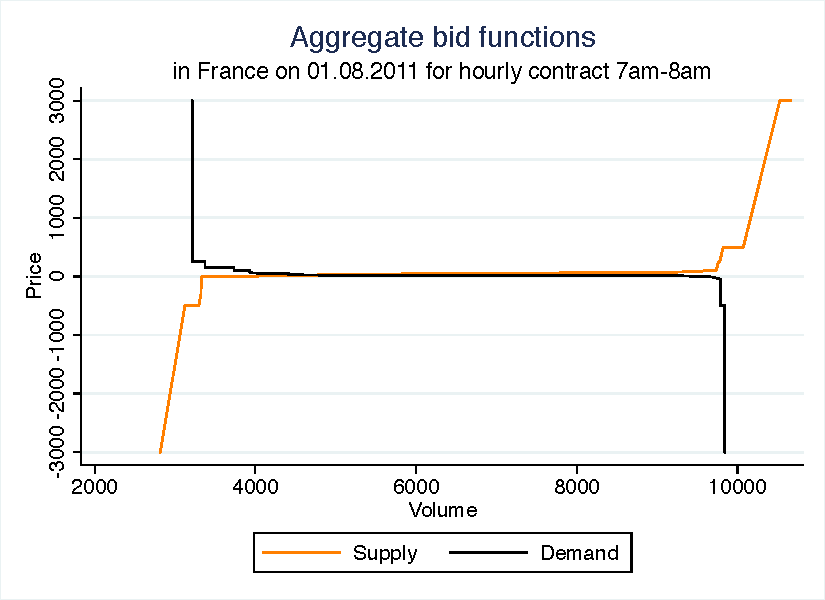
\includegraphics[height=50mm]{figch2/aggbidfuncnozoom.pdf} \hspace{0.05cm}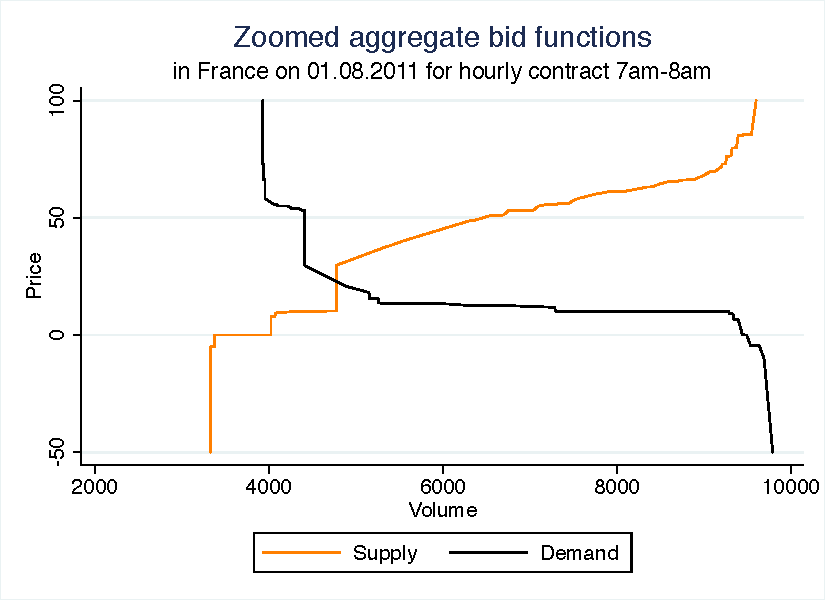
\includegraphics[height=50mm]{figch2/aggbidfuncwithzoom.pdf} \end{center}
\caption{Example aggregate demand and supply bid functions}
\label{examplebidfunc}
{\small Note: The right-hand-side graph is a zoom of the left graph on for the price range  $-50$\EUR{}/MWh  to +100\euro /MWh.}
\end{figure}


\begin{figure}[!ht]
\vspace{0.3cm}
\begin{center}\makebox[\textwidth][c]{
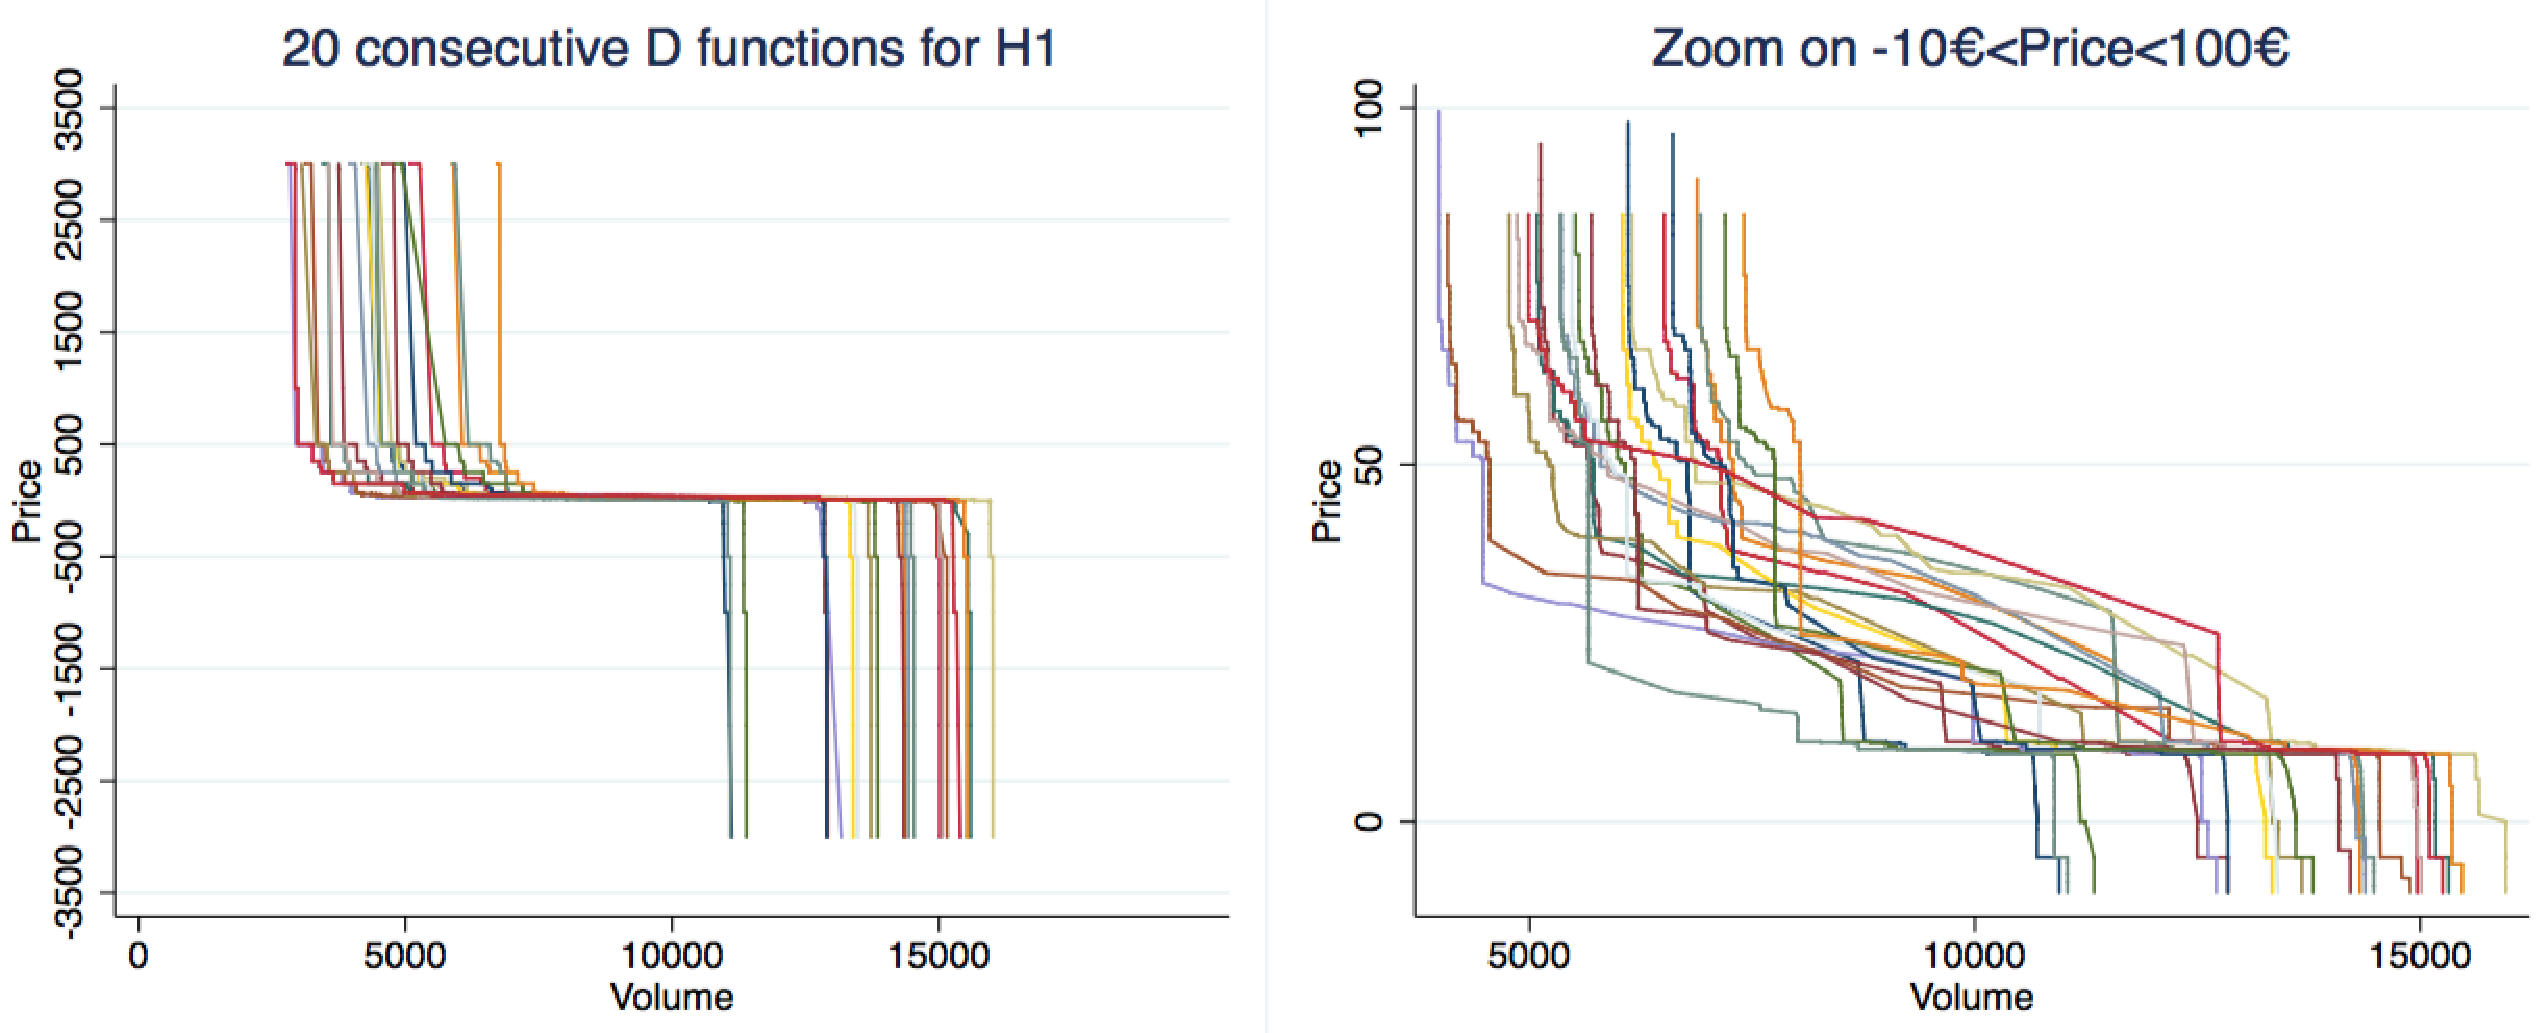
\includegraphics[height=50mm]{figch2/Shot28.pdf}
}\\
\vspace{0.05cm}
\makebox[\textwidth][c]{
\includegraphics[height=50mm]{figch2/Shot27.pdf}
}
\caption{Aggregate bid functions for 20 consecutive days}
\label{graphmultifunc}
\end{center}
{\small Note: The graph shows 20 consecutive aggregate demand and supply functions for the contracts on hour 1 (between 12am and 1am) for the time period 11/12/2011 to 31/12/2011. The graph on the right is a zoom on the price elastic region of the curves on the left.}
\end{figure}

	%%%%%%%%%%%%%%%%%%%%%%%%%%%%%%%%%%%%%%%%%%%%%%
	% Tabular data to give an example
	% Keep LONGTABLE TO HAVE FOOTNOTES APPEAR. 
	%%%%%%%%%%%%%%%%%%%%%%%%%%%%%%%%%%%%%%%%%%%%%%	
%\setlength{\LTleft}{-20cm plus -1fill}
%\setlength{\LTright}{\LTleft}
%\setlength{\LTpre}{18pt}
%\setlength{\LTpost}{0pt}
%\newgeometry{margin=2cm} 
%\begin{landscape}
%\footnotesize
%\begin{table}[!ht]
%\vspace{-1.4cm}


\begin{center}
% matrix: out1 file: /Users/Orie/Cloud/Google Drive - Account henridb1/Encheres Elec/Article/overallsummary.tex   1 Oct 2014 15:48:56
\begin{center}
\begin{longtable}{lrrrrr}
\toprule
 & Mean  & Median  & Std. Dev  & Min  & Max  \\
\midrule
\endfirsthead
\multicolumn{6}{l}{\emph{... table \thetable{} continued}} \\
  & Mean  & Median  & Std. Dev  & Min  & Max  \\
\midrule
\endhead
\midrule
\multicolumn{6}{r}{\emph{Continued on next page...}}
\endfoot
\endlastfoot
Total daily volume &  161,912 &  159,313 & 25,059 & 99,054 &  277,531 \\  
Average realised daily price\footnote{Average price is volume weighted over the 24 hourly contracts of the delivery day.} &    46.6 &    48.3 &    17.2 &   -39.0 &   381.2 \\  
%Congruence ratio\footnote{It is defined by the ratio of maximum supplied volume to maximum demanded volume. It is based on \cite{armstronggalli2007empirical} and measures liquidity in the market by comparing how similar buyer and seller attitudes to trade are on the market. The authors find that unusually high prices generally occur when this metric exceeds 2.} &     1.11 &     1.07 &     0.32 &     0.45 &     4.51 \\  
Minimum demanded agg. volume\footnote{Minimum and maximum volumes for both demand and supply refer to the aggregate volume bid on the market for a single hour contract at the extremal prices of $+3000$\euro /MWh or $-3000$\euro /MWh.} & 5,030 & 4,968 & 1,467 &   914 & 11301 \\  
Maximum demanded agg. volume & 13,327 & 13,222 & 2,212 & 4,990 & 23,254 \\  
\midrule
Minimum supplied agg. volume & 3,721 & 3,526 & 1,344 &   618 & 10594 \\  
Maximum supplied agg. volume & 14,390 & 14,142 & 3,051 & 6,580 & 35,356 \\  
Bid points per demand function &   543 &   531 &   163 &   115 & 1,253 \\  
Bid points per supply function &   640 &   632 &   143 &   184 & 1,283 \\  
Bidders per auction\footnote{Due to the anonymity of the auction procedure, it is unknown which bidders submitted bids. Consequently, it cannot be deduced how many bid steps a typical bidder submits. Number of registered bidders for the French EPEX Spot market as of 01.10.2014.} &   - &    - &   - &   1 & 101 \\
\bottomrule
\caption{\label{overallsummary} Some descriptive statistics}
\end{longtable} 
\end{center}
%\caption{\label{overallsummary} ***}
\end{center}
%\emph{Note}:
%\end{table}
%\end{landscape}
%\restoregeometry


		%%%%%%%%%%%
		% can include more info on number on functions observed and give 
		% tabular stata at 3 year level for weekday only. 
		% say we focus on weekdays, not distinction between mo and tues
		%%%%%%%%%%
\subsection*{Exogenous factors}
	%%%%%%%%%%%%%%%%%%%%%%%%%%%%%%%%%%%%%%%%%%%%%%
	% Meteo data
	%%%%%%%%%%%%%%%%%%%%%%%%%%%%%%%%%%%%%%%%%%%%%%

Regarding weather statistics, we have hourly previsions for temperature, wind and cloudiness from the GFS (Global Forecast System) as well as hourly observations for these quantities and luminosity from M\'{e}t\'{e}oFrance
. The previsions from the GFS are in the form of weather maps that are outputted from simulations that run one-day ahead at 6 am. This is the weather information that market participants have access to when bidding on EPEX Spot\footnote{The next weather simulation run takes place at 12 noon, and is therefore not being used by the bidders on the EPEX day-ahead market, as the deadline for submitting bids is precisely 12 noon.}. The weather observations are in the form of tables for specific weather stations (between 100 and 200 depending on the specific parameter of interest).\\

Moreover, we have the location of the total installed capacity per generation type (i.e. wind turbines, solar panels, etc.) at the level of the postcode, that is roughly a 3km precision. We obtain this data from the SOeS, a branch of the French government producing data on environmental issues at large. \\

Population data and data on the level of the domestic production from the manufacturing industry is obtained in monthly steps from the French National Institute of Statistics and Economic Studies (INSEE). From the same source, we obtain the spot prices for petrol and natural gas as well as the import prices at the border for coal, which we use as a proxy for the domestic prices. 
Prices for the European CO2 emission certificates are taken from the Portuguese secondary market (SENDECO$_2$) for European Unit Allowances (EUA)\footnote{Each unit EUA permit allows one tonne of CO2 emissions.}.\\

As a very coarse proxy for generation from hydro power plants, we have the total weekly stock of water in domestic dams (in the form of the summed height of all dam water levels in France) from RTE the grid operator.


\section{Methodology}
\label{newapproach}
We want to identify the impact that the level 
%and growth (positive or negative) 
of 
%residual demand 
uncertainty has on the price elasticity of the aggregate supply function. In data terms, this means that we aim to regress the slope of (aggregate) supply bid functions on a proxy corresponding to the uncertainty that existed at the time of bidding. The uncertainty may come from two different sources: (i) uncertainty about the realization of market demand and (ii) uncertainty on the generation from renewables. Both types of uncertainty affect the residual demand curve faced by each supplier\footnote{Renewable generation benefits from a feed-in guarantee on the market and thus reduces the residual demand for all traditional electricity producers.}.\\

This regression is able to explain how supply firms adjust their bidding strategies to the expectation of demand shocks that they face. Statistical significance of the level of uncertainty on the slope of the supply function would be evidence that firms take the strategic considerations of dynamic costs into account. \\

%We first outline the strategy of our work in section \ref{strat}. In section \ref{identification}, we then detail the identification of the effects we are interested in. Section \ref{comparablepoints} addresses methodological details. 

%\subsection{Outline of methodology}
\label{strat}
%Three questions compose this project: First, how to appropriately extract the price elasticity of the supply function. Second, how to obtain a natural, precise (and exogenous) measure of the uncertainty. Third, how to test the former on the latter using a simple technique.

First, in section \ref{identification} we show the final regression of interest. Sections \ref{LHS} and \ref{RHS} then detail the theory and empirics underlying the variables that feed into the final regression. \\

Some of the information used in our analysis is drawn from the bid functions of the EPEX Spot market. As introduced in section \ref{datasection}, we observe the full aggregate %\footnote{However, we do not observe individual bid functions (which would have been even better).} 
bid functions for both supply and demand, %This is particularly suited for our analysis, since it allows to condition our analysis on specific points of the functions.   
%This is useful as show the graphs in figure \ref{graphmultifunc} since 
the shape of which %the supply bid functions 
(and thus the information that we aim to extract from them, e.g. their slope) varies differently at different points (recall the graphs in figure \ref{graphmultifunc}). \\%(the same goes for the demand function and the measure of the uncertainty). 
%Therefore, an overarching question is how to make sure that we can compare specific bid points from one auction to the next and that we use corresponding measures in the regression. The that 
Generally speaking, a regression aims at quantifying the impact of some independent variables on a dependent one. The dependent variable is most frequently numerical, and the independent variables explain part of its value. Here the dependent variable is functional in nature, that is that we aim to describe how the supply function changes shape with respect to some independent variables. One observation is formed of one function coupled to the value of some independent variables. We therefore adopt a functional data analysis approach, which allows us to condition our analysis at specific points $k=1,..,K$ of the functions.
% The specific points $k=\{1,...,K\}$, chosen to base our analysis on, 
This approach allows to define comparable points across auctions, that is different functions, in order to derive insights.   \\
%do this cross-auction comparison. 

More precisely we want to quantify how uncertainty affects the strategy of bidders from one hour to the next. For this we cannot rely on a standard estimation of the overall demand or supply functions from market outcomes, we want to actually measure how the functions that we observe change shape. \\

The methodology to select comparable points across auctions is detailed in chapter 2. 
This appendix also evaluates the results when applying the technique to our data from the Epex Spot market. Figure \ref{TypeallocK} shows the selected points on an exemple of demand and supply curve. \\

The different types of points selected capture different information of the aggregate bid functions. The most important point is the one we label $k=3$, which corresponds to the central part of the bids. This point is most relevant for equilibrium determination \footnote{See figure \ref{g7f} for a glimpse at the distribution of equilibrium outcomes.}. The points $k=2,4$ are the points of maximum curvature and represent the transition points between the central (very price elastic) region and the outer (very price inelastic) regions of the bid function. Last, we have the points $k=1,5$ which are imposed by the auction rules and are the endpoints of the bid functions. \\

\begin{figure}[!ht]
\begin{center} 
\makebox[\textwidth]{
\includegraphics[height=50mm]{figch2/DemandplusK.pdf} 
\hspace{0.05cm}
\includegraphics[height=50mm]{figch2/SupplyplusK.pdf} 
} 
\end{center}
\caption{Selected points on original bid functions}
\emph{Note: } The demand function left, the supply function right, the graph superposes and names the points selected according to the methodology of section \ref{newapproach}.
\label{TypeallocK}
\end{figure}
 
In chapter 2, we also detail the choice of setting $K=5$ and show that this choice allows us to improve the precision of our analysis by a factor of 50 when it is conducted on the 5 points simultaneously\footnote{We briefly mention that the evaluation of the point selection has revealed focal price points for the points $k=2,4$. These points are however rarely relevant for equilibrium determination.}.
%**** CHECK ALEX \footnote{alternative:  *****reduce the degrees of freedom of bid function volatility by a factor of about $50$ as compared to selecting a single point}. 



\subsection{Regression methodology}
\subsubsection{Identification}
\label{identification}
	%%%%%%%%%%%%%%%%%%%%%%%%%%%%%%%%%%%%%%%%%%%%%%
	% Methodology
	%%%%%%%%%%%%%%%%%%%%%%%%%%%%%%%%%%%%%%%%%%%%%%	
At each of these comparable points, %$k=\{1,..,K\}$, %we use a two stage least squares methodology, where the first stage produces a natural measure of the uncertainty that producing firms have and the second stage 
we want to identify the effect of uncertainty on the slope of the supply function. \\%The regression runs over all auctions $i=\text{Hour 1 on }01.01.2011, ..$. %, for convenience we drop the index $i$.

%\subparagraph{In the second stage,} we want to measure the impact of the constructed uncertainty proxies on the price elasticity of supply. 
%By the same methodology as in step one, we extract the slope of the supply bid function a $m$ points and use this as our local proxy for the price elasticity of supply. 

Defining $S'_{i,k}$ the slope of the supply function of auction $i$ at point $k$ in the quantity (X-axis) - price (Y-axis) dimension, %$\boldsymbol{\epsilon^D_{i(H)}}$ being the vector of residuals from the price (equation \ref{regDP}) and the volume prediction (equation \ref{regDQ})
$\boldsymbol{X^S}$ being the vector of exogenous variables, PLU$^D_{i,k}$ being the proxy for the level of demand uncertainty, PLU$^R_i$ being the proxy for the level of uncertainty from renewables, $\alpha$ being the regression constant and $\epsilon$ being the error term%and PDU being the proxy for the dynamics of the uncertainty
, we estimate the following:
%\begin{eqnarray}
%\label{secondstagereg2b}
%S'_m(H) &=&\alpha_{m(H)}^S+ \boldsymbol{\beta_{i,m(H)}^S}\sum_{i=1}^{K} V(\boldsymbol{\epsilon_{i(H)}^D}) \nonumber \\  &+&\boldsymbol{\eta_{i,m(H)}^S}\sum_{i=1}^{K} \Delta V(\boldsymbol{\epsilon_{i(H)}^D})+ \boldsymbol{\gamma_{m(H)}^S X}+\epsilon_{m(H)}^S
%\end{eqnarray}
\begin{eqnarray}
\label{secondstagereg2}
S'_{i,k} =\alpha_{k}^S+ \beta_{k}^S \text{PLU}^D_{i,k} + \gamma_{k}^S \text{PLU}^R_{i} + \boldsymbol{\delta_{k}^S X^S_i}+\epsilon_{i,k}^S
\end{eqnarray}

We are interested in the sign and magnitude of the coefficients $\beta^S$ and $\gamma^S$, which identify the effects of the PLUs (PLU$^D$ and PLU$^R$, respectively) on the shape of the supply bid function. From the predictions outlined in section \ref{intropredict}, we expect a positive coefficient when uncertainty levels increase\footnote{Specifically, we want $\beta^S$ to be positive, $\gamma^S_1$ positive and $\gamma^S_2$ negative. For details on $\gamma^S$, see section \ref{proxyautocorrel}.}.\\ %\cite{bergesmartimort2014}  predict a positive $\eta_Q$ since the model only allows for quantity shocks to demand. 

%In equation \ref{secondstagereg}, we ignore the dynamic uncertainty in price prediction $\Delta V(\epsilon_{P_k(H)}^D)$. This is because \cite{bergesmartimort2014} only allow for quantity shocks to demand. An extension will control for the impact of price uncertainty. 



\subsubsection{Left-hand-side variables}
\label{LHS}
We extract the slope of the aggregate supply function at any given point $k$ from a kernel density estimation with a bandwidth of 45 units\footnote{The
slope is a by-product of the point selection mechanism and the bandwidth selection for the smoothing thus follows the same considerations as for the latter. The details of this choice are specified in chapter 2.}.  \\

Effectively, this is a smoothed version of the slope. This makes our slope estimates robust to steps in the bid function\footnote{In our data, we observe that bid functions are effectively step functions. On EPEX spot $256$ price-quantity combinations are allowed per bidder. When additional bid points are costly, then stepwise bidding behaviour may be very different from a setting where continuous functions can be bid \cite{kastl2011discrete}. Due to the fact that, on average, we do not observe that firms use up all available price-quantity combinations , the cost argument of an additional bid point seems weak. Hence, by smoothing the slope we approximate the unconstrained, continuous bid function. }, which in turn allows us to test the predictions from the theoretical paper. 
Steps in the bid functions mostly are much larger towards the extremities of the bid functions and probably arise from capacity constraints considerations. 
Working with smoothed slopes is  in line with previous work \`{a} la \cite{pw2002etude} and \cite{ozcan2004logistic}, who also apply reduced form models to aggregate bid function data. 


\subsubsection{Right-hand-side variables}
\label{RHS}

We are regressing an ex-post measure of the auction market (realised slope of the supply bid function) on ex-ante information that bidders have at the time of bidding, i.e. which is available at midday of the day ahead of delivery.  
We thus keep a strict separation of the ex-post and  ex-ante information to the left  and right hand side of equation \ref{secondstagereg2}, respectively. This separation allows us to circumvent endogeneity problems and  validates the use of simple OLS regressions. \\

For this reason, we construct our PLUs on the basis of predicted uncertainty. However, for data availability reasons we cannot exclude endogeneity problems completely. For details, see the discussion in section \ref{endogeneityconcern}.  \\

In this subsection, we first outline how we generate the proxies for the level of market demand uncertainty (PLU$^D$) in section \ref{proxyunc}. Second, we construct the proxies for the level of uncertainty from renewables energies (PLU$^R$) in section \ref{proxyautocorrel}. Third, we detail how the vector of exogenous variables ($\boldsymbol{X}$) is constructed in subsection \ref{controlssec}.  \\


\subparagraph{Generating proxies for uncertainty from market demand (PLU$^D$)}
\label{proxyunc}

We construct a proxy for the level of the demand uncertainty (PLU$^{D}$) by using the residuals from a demand estimation on exogenous parameters as a measure of the uncertainty that bidders face in an auction. Specifically, our PLU$^D$ is the expected squared level of the prediction errors that firms expect to make when anticipating the demand level of the day ahead. We assume that the ex-post prediction errors give a reasonable estimate of the uncertainty at the time of bidding. \\



%%In order to make full use of the data variability in the dataset, the PLU$_i$ encompasses the whole uncertainty (at the $K$ comparable points) of the demand function, since we do not have a priori knowledge of any specific local uncertainty (e.g. uncertainty at the boundaries or towards the point of intersection) driving the effects. 
%The uncertainty proxies are given by 
%the point-specific PLU$_{D,i,k^{-1}}$  is given by  $ V(\epsilon^D_{i,k^{-1}}) $, a measure of the variation of demand prediction errors: 
%\begin{equation}
%\label{levelproxy}
%\text{PLU}_{D,i,k^{-1}} 
%= V(\epsilon^D_{i,k}) 
%\end{equation}
%%\begin{equation}
%%\label{dynamicsproxy}
%%\text{PDU} = \sum^K_k\text{PDU}_{k} = \sum^K_k \Delta V(\epsilon^D_{k}) 
%%\end{equation}

The uncertainty proxy
%individual, point-specific proxies (PLU$_{i,k}$) 
is obtained as detailed next in a three-step procedure. In the first step, we explain what kind of uncertainty our PLU$^D$ refers to. The second step details the conceptual details of constructing the PLU$^D$. The third step computes the PLU$^D$. % and the fourth computes the proxy of the dynamcis of uncertainty (PDU). 

%We then compute the variation of these variances over time, $\Delta V(\epsilon_{P_k(H)}^D)=V(\epsilon_{P_k(H)}^D)-V(\epsilon_{P_k(H-1)}^D)$ and $\Delta V(\epsilon_{Q_k(H)}^D)=V(\epsilon_{Q_k(H)}^D)-V(\epsilon_{Q_k(H-1)}^D)$  as a proxy for the dynamics of the uncertainty.
%*** V and $\epsilon$ missing the index for P or q dimension - on purpose.

\subparagraph{In the first step,} 
\label{firststepresiduals}
we focus the analysis to a fixed number $K$ of comparable points across auctions by using the non-parametric point selection technique outlined in section \ref{newapproach}. 
Each k$^{th}$ point is defined by a price and a quantity, which we regress independently on the exogenous variables. \\% for each auction $i$ (for which we now drop the index). 

Let us call $P_{i,k}^D$ and $Q_{i,k}^D$ the price and quantity of point $k$ of the realised demand function in auction $i$, $\boldsymbol{X^D_i}$ the vector of exogenous variables relevant for the demand estimation.
%\end{siderules}
\begin{eqnarray}
P_{i,k}^D=\alpha_{k}^{D,P}+{\boldsymbol{\beta_{k}^{D,P}}} \boldsymbol{X^D_i}+\epsilon_{i,k}^{D,P} \label{regDP}\\
Q_{i,k}^D=\alpha_{k}^{D,Q}+{\boldsymbol{\beta_{k}^{D,Q}}} \boldsymbol{X^D_i}+\epsilon_{i,k}^{D,Q} \label{regDQ}
\end{eqnarray}
In regressions \ref{regDP} and \ref{regDQ}, firms try to anticipate the realisation of the demand using the exogenous information available. We consider that the producers are able to do such an analysis at the time of bidding. \\%\footnote{We avoid the use of hour dummies by controlling for the time of the day using the variables suncycle, morning, deltasun. For details, see section \ref{controlssec}. }

The prediction errors  $\epsilon_{i,k}^{D,J}, \; J=\{Q, P\}$ are a consequence of the stochastic nature of the demand and hence a manifestation of the uncertainty. We consider that more uncertainty will lead to larger prediction errors being made in equilibrium and adopt the 
square
%standard deviation 
of the residuals $ \bigl( \epsilon_{i,k}^{D,J} \bigr)^2$ as our measure for the realised level of demand uncertainty.%PLU$^D_{i,k}
.

%\footnote{Dropping the indices $D$ and $J$:% and $k$):
%\begin{equation}
%\label{eqnstandarddevofres}
%\text{PLU}_{i,k} = \sigma\bigl( (\epsilon_{i,k})^2 \bigr) = \sqrt{\sum^n_{i=1}\frac{\bigl(\epsilon_{i,k}^2 - \overline{\epsilon_k^2}\bigr)^2}{n}}
%\end{equation}
%%\begin{equation}
%%\label{eqnstandarddevofres}
%%\hat{\text{PLU}} = \sigma\bigl( (\epsilon_{i,k}^{D,J})^2 \bigr) = \sqrt{\frac{1}{N}\sum^N_{i=1}\bigl((\epsilon_{i,k}^{D,J})^2 - (\overline{\epsilon_{i,k}^{D,J}})^2\bigr)}
%%\end{equation}
%The sample size $n$ refers to the fact that the PLU$_{i,k}$ is measured over similar auctions only. }.


\subparagraph{In the second step,} 
\label{secondstepresiduals}
%we compute the variances of the predicted residuals conditional on the exogenous variables and consider this a good proxy of the level of uncertainty faced by the producers that we denote $V(\epsilon_{P_k(H)}^D)$ and $V(\epsilon_{Q_k(H)}^D)$. The underlying hypothesis is that more uncertainty will lead to larger prediction errors being made in equilibrium.

%\subparagraph{Bin based variance estimates}
%\label{binbasedvariances}
%Step 1: Predict Price and Volumes from Demand estimation as in euqations \ref{regDP} and \ref{regDQ}. 

we recover the residuals from the demand estimation in regressions \ref{regDP} and \ref{regDQ} and test for heteroskedasticity using \cite{white1980heteroskedasticity}, which is clearly confirmed (see tables \ref{VolDEPur52} and \ref{PriceDEPur52}). \\

Heteroskedasticity means here that the variation of error terms varies conditional on the levels of the exogenous factors: $E(\epsilon_i^2 \vert \boldsymbol{X_i})=g(\boldsymbol{X_i})$. However, they are still orthogonal%have tested and error terms are orthogonal both individually as well as collectively. 
: $E(\epsilon_i \vert \boldsymbol{X_i})=0$, thus ensuring that the prediction is unbiased, but not ``best" in the sense of the best linear unbiased estimator (BLUE). Thus, heteroskedasticity results in inefficient regressions where the estimator is not minimum variance. 
%*** CITE. 
Since we do not interpret regressions \ref{regDP} and \ref{regDQ} for causality, but only for predictive purposes, we stick to the unbiased OLS. \\

The heteroskedasticity regression is given for $J=\{P,Q\}$ by
\begin{equation}
\label{heteroskedeqn}
 \bigl( \: \epsilon_{i,k}^{D,J}\: \bigr)^2= \alpha^{U,J}_{k} + \beta^{U,J}_{k} \boldsymbol{X^D_i} 
 +\epsilon^{U,J}_{k}
\end{equation}



\subparagraph{In the third step,} we compute the predicted PLU$^D_{i,k}$ that firms use when bidding in the auction as:
\begin{equation}
\label{predictu}
 \underbrace{ \widehat{ \bigl( \: \epsilon_{i,k}^{D,J}\: \bigr)^2}}_{\widehat{\text{PLU}}^D_{i,k}}= \alpha^{U,J}_{k} + \beta^{U,J}_{k} \boldsymbol{X^D_i} 
 % +\epsilon^{U,J}_{k}
\end{equation}
The idea is that by experience, firms in the market know that their predictions are more or less accurate depending on the environmental conditions (in the sense of realisations of exogenous factors%(e.g. similar temperature, windproduction, etc...)
). In other words, firms can use the realisations of $ \boldsymbol{X^D}$ to infer the accuracy of their demand predictions. %, i.e. the expected confidence interval on their prediction. 
 Technically speaking, they can use the heteroskedastic nature of the residuals to forecast the level of uncertainty that they face.\\


The PLU$^{D}$ subs into regression \ref{secondstagereg2}. 
For simplicity, we do not include the uncertainty proxies PLU$^D_{i,k}$ measured at all $K=5$ points in regression \ref{secondstagereg2} simultaneously, but only a single PLU$^D_{i,k}$ at a time. 
Therefore in the final regression \ref{secondstagereg2}, we regress the slope at a point of the supply function on the PLU$^D_{.,.}$ estimated at the corresponding point on the demand function. The pairing is done in the quantity dimension. This means that the slope of the supply function at point $k=2$ is regressed on the uncertainty measured at point $k=4$ of the demand function (recall the labelling of the points as given in figure~\ref{TypeallocK}). We indicate this quantity paring in the index $k^{-1}$ of the PLU:
\begin{equation}
\label{levelproxy}
\text{PLU}^D_{i,k} = 
\widehat{\text{PLU}}^D_{i,k^{-1}} 
%= \bigl(\widehat{\epsilon}^D_{i,k^{-1}}\bigr)^2 
\end{equation}
An increase in PLU$^D_i$ corresponds to an increase in the uncertainty about the market demand realisation. We thus expect $\beta^S$ to be positive in regression \ref{secondstagereg2}.


\subparagraph{Generating proxy for uncertainty from renewable energies (PLU$^R$)}
\label{proxyautocorrel}

We have already referred to the statement that the intermittency of renewables causes large residual demand shocks \cite{epexwebsite1}. Suppliers are thus wary of the expected production of renewables generation. \\

Given that renewable generation is an exogenous source of supply, it affects the residual demand curve for each supplier, but does not enter the PLU$^D$, which captures the uncertainty on market demand only. \\

In predicting the generation from renewables, we assume that suppliers are able to infer renewables generation from meteorological forecasts\footnote{We specify the technique in chapter 2 and use it to construct our controls in section \ref{controlssec}.}.\\

When forecasting the residual demand shocks due to generation from renewables, we consider that suppliers have an idea of the precision of their estimate based on the ``look" of the meteorological forecasts that they have. By look, we mean the geographical heterogeneity or homogeneity of the forecasts, i.e. if when looking at a weather map, one sees a lot of spatial variations or not. \\

We consider that this notion of geographical heterogeneity of the forecasts correlates to the uncertainty associated with the prediction of renewable production. The argument is as follows: \\
\textbf{First}, renewable production is built by aggregating the forecast of all individual renewable sources. This means knowing the position and capacity of every renewable source, querying weather forecasts for all of these points, modeling the renewable's response to the forecasted weather, and adding the forecasted productions. \\
\textbf{Second}, we note that weather is spatially correlated, which means that the closer two points are, the closer the values for a given weather variable (the air temperature at your left hand is very close to that at your left hand, but less so across the city, and even less so across the country). This correlation roughly follows an exponential law : the difference between the values of a weather variable between two points behaves in a linear fashion for small distances, and saturates at large distances \footnote{Intuitively, the characteristic lengthscale of autocorrelation represents the distance required between two geographical points on a map of weather forecasts to observe a decorrelation of half of its maximum value. For example on the wind speeds prediction, a characteristic length of 80 km means that if we observe two very distant points (say 1000km) to have a difference in wind speeds of, on average, 50km/h (this being the maximum difference, we are in the saturated regime), then we will observe, on average, wind speed differences of 25km/h for points distant from each other by 80km.}. The transition between those two regimes is given by a caracteristic lengthscale, a bit less than 200km on average. \\
\textbf{Third}, we observe that the average distance between production points is large enough that the relevant regime of autocorrelation is the saturated part \footnote{For N production points, we compute the N(N-1)/2 pairs of points, consider their distances, and compute the average of these distances weighted by the production capacity at every point. In the case of the wind we have an average distance of 459 km, in the case of the photovoltaic production we have an average distance of 499km.}. \\
\textbf{Fourth}, we note that there are two main channels through which the overall uncertainty about renewable production is related to the weather. There is an issue of error averaging, which means that if the weather becomes very spatially uncorrelated, one can expect errors to cancel out relative to a given bias in the forecast. This channel would tend to imply that more spatial variations imply a smaller uncertainty about production. There is also the issue that weather forecasts are numerical simulations and that the mesh size for such simulations, typically 5km for the high precision ARPEGE model of Météo France, implies that the errors are higher as the simulated phenomenons have higher gradients. This means in our case that the uncertainty about the forecast increases as the weather becomes more spatially uncorrelated. \\
\textbf{Fifth}, these two effects are of opposite signs, but our third point is an argument for considering that the averaging of errors is smaller than the simulation errors. Therefore we expect our uncertainty to increase as the spatial autocorrelation decreases (i.e. more spatial variation). \\

This can be summed up with the following hand-waving argument : when there is more spatial variations, the weather is more messy, therefore more difficult to predict. \\

We compute this characteristic lengthscale ($L$) as described in chapter 2. Our PLU$^R$ is defined as the two proxies 
\begin{align}
 \text{PLU}^R_{1,m} &= \frac{1}{L_m}, \quad \quad  \text{where } m=\{\text{Wind, Solar, Temperature}\} \\
  \text{and }  \quad \text{PLU}^R_{2,m} &=  \bigl(\frac{1}{L_m}\bigr)^2
\end{align}

As explained above, we expect firms to face less uncertainty in predicting weather conditions when the lengthscale of autocorrelation $L$ is longer since the overall weather conditions will be more homogenous. A longer length $L$ (less uncertainty), will yield a smaller PLU$^R$ and we expect a flattening of the supply curve. I.e. we expect a positive coefficient $\gamma^S_1$ on the PLU$^R_{1,m}$ variables in the final slope regression.\\

However, we also expect to the effect of $L$ on the slope to be attenuated, if not counterbalanced, by the squared term\footnote{We expect the effects of $L$ on the slope to be of the shape of a Laffer curve.}. This means that for very small $L$, we expect an additional effect, that of the summation of errors, to become significant and reduce the uncertainty, or at least its rate of increase: we thus expect a negative coefficient $\gamma^S_2$ on the squared PLU$^R$ term in the final slope regression (equation \ref{secondstagereg2}). 

\subparagraph{Controls}
\label{controlssec}

This section details the exogenous variables, which we use for our study. The stacked vector of exogenous variables is not identical for the supply and demand regressions of equations \ref{secondstagereg2} and \ref{regDP}.\\ 

The vector $\boldsymbol{X^D}$ for the demand equation includes the variables: Tempeff15, Roll\_Temp24, Roll\_Temp240, suncycle, morning, deltasun, EWH, SolarRest, RteBlackBox.\\

For the supply regression we include in $\boldsymbol{X^S}$ the following variables\footnote{We do not include the variables used for the demand estimation as they indirectly feed into the final regression via the PLU$^D$.}: 
Coal, Brent, Gas, IT2, EUA, Wind1DA, Hydro. \\
 
Table \ref{exogsummary} gives a brief overview of the controls used. Details on the computation of some  variables are given in the appendix (see links in table). The last column indicates the frequency with which we observe the variable in question. 

\begin{center}
\begin{longtable}{p{2cm} p{8.5cm} p{1.3cm}  p{1.5cm}}
 \multicolumn{1}{l}{Name}   & Explanation & Unit  & Frequency \\
\midrule
 \endfirsthead
\multicolumn{3}{l}{\emph{... table \thetable{} continued}} \\
 \multicolumn{1}{l}{Name}   & Explanation  & Unit  & Frequency \\
\midrule
\endhead
\midrule
\multicolumn{3}{r}{\emph{Continued on next page...}}
\endfoot
\endlastfoot
Wind1DA & The day-ahead predicted electricity volume generated from wind turbines. 
Details on p. \pageref{Wind1DA}. & MWh  & Hourly   \\
\midrule 
Solar & The electricity volume generated from photovoltaic sources. 
Details p. \pageref{Solar} & MWh &  Hourly \\  
\midrule
%Tempeff & 
%Predicted temperature in France, aggregated on a national level. 
%Details on p. \pageref{Tempeff}. & $^\text{o}$C & Hourly\\
%\midrule 
% Roll\_avgT24 & Mean of \emph{Tempeff} over the last  24 consecutive hours. Details on p. \pageref{}. &  $^\text{o}$C   & Hourly \\
%\midrule
% Roll\_avgT240 & Mean of \emph{Tempeff} over the last  240 consecutive hours. Details on p. \pageref{}.  &  $^\text{o}$C  & Hourly \\
%\midrule
Tempeff15 & 
Effective predicted temperature in France (with a cutoff point at $15^o$C to reflect demand patterns), aggregated on a national level.
Details on p. \pageref{Tempeff15}. & $^\text{o}$C & Hourly\\
\midrule
 Roll\_Temp24 &  Mean of \emph{Tempeff15} over the last 24 consecutive hours. %Details on p. \pageref{}.
  &  $^\text{o}$C   & Hourly \\
\midrule
 Roll\_Temp240 & Mean of \emph{Tempeff15} over the last 240 consecutive hours. %Details on p. \pageref{}. 
 &  $^\text{o}$C   & Hourly\\
\midrule
suncycle & Luminosity as a percentage of maximum luminosity of the day. %Proxy for time of the day as a function of the cycle of the sun. 
\emph{Midday} defined as \emph{suncycle}=1. Details on p. \pageref{suncycle}.  & $\%$ & Hourly\\
\midrule
 morning & Indicator variable for hours before \emph{Midday}. %Details on p. \pageref{morning}. 
 &$ \{0,1\}$ & Hourly\\
\midrule
 deltasun & Absolute value of the change in \emph{suncycle}.  Details on p. \pageref{deltasun}. & $ [0,1]$ & Hourly\\
 \midrule 
 EWH & Indicator variable for hours between 10pm and 4am. % Details on p. \pageref{EWH}. 
 & $ \{0,1\}$ & Hourly\\
 \midrule
SolarRest & The unexplained component of photovoltaic generation. Specifically, the residuals from a regression of \emph{Solar} on \emph{suncycle}. Details on p. \pageref{SolarRest}. & MWh &  Hourly \\  
\midrule
RteBlackBox & The unexplained component of the day ahead prediction of total consumption in France issued by the grid operator (RTE). Specifically, the residuals from a consumption estimation. Details on p. \pageref{RteBlackBox}. & MWh &  Hourly \\  
\midrule
Coal  & Average coal import prices at the French border. %Details on p. \pageref{Coal}. 
& \EUR{}/ton &  Monthly \\  
\midrule
Brent & Average of spot prices for crude oil on the London based stock exchange.% Details on p. \pageref{Brent}. 
& \$/bl & Monthly\\
\midrule
Gas & Average of closing prices for natural gas at 1 month on the London market (NBP). %Details on p. \pageref{Gas}.  
& \textsterling/Therm &  Monthly \\  
\midrule
IT2 & Interaction term between gas and demand: \emph{Gas} weighted by an hourly index for the demand level \footnote{Gas turbines generate electricity using natural gas as a fuel. We thus proxy for its input price using a Gas variable for which we take the closing price for natural gas at 1 month on the London market (NBP). Electricity generation from gas is expensive and flexible. In general gas plants are only called upon to provide peak load electricity generation in moments of high demand. WE therefore compute an interaction term between Gas and an index for the hourly level of the demand. The index acts as a weight on the gas price. The weight is computed as the percentage demand level as compared to the maximum demand level observed in our dataset.} & \textsterling/Therm &  Hourly \\  
\midrule
EUA  & Price of CO$^2$ emissions. %Details on p. \pageref{EUA}. 
& \EUR{}/ton &  Daily \\  
\midrule
Hydro & Sum of dam level heights on a national level. %Details on p. \pageref{Hydro}.
& $\%$ &  Weekly \\  
\midrule
\bottomrule
\caption{\label{exogsummary} Overview of exogenous variables.}
\end{longtable} 
\end{center}


The rationale for the included variables is the following: \\

First, Wind1DA and Solar control for the expected level of renewables generation\footnote{For data availability reasons, Solar is computed on realised luminosity values rather than forecasts of luminosity.} on the day ahead market. These are computed using a novel bottom-up methodology described in the appendix \ref{interpmethodo}. \\

Second, Tempeff15 controls for the demand patterns as a function of the temperature\footnote{Note that electric heating is widely spread in France. It is used in 32\% of principal residences (INSEE, RP2011 exploitation principale).}. 
Tempeff15 includes a cut-off at $15^o$C in order to take into account the demand pattern as a function of temperature according to \cite{rtewebsite1}. Table \ref{black1} reveals the improved fit over a simple temperature variable without respecting the demand cut-off (Tempeff). \\

Third, Roll\_Temp24 and Roll\_Temp240 capture the demand seasonality via the temperature. The former gives the daily average temperature, while the latter captures the average temperature over the last 10 days. The demand cut-off at $15^o$C for Tempeff15 is respected for these means.  Including these as seasonality controls allows to get away from using dummy variables for the seasonality. In short, avoiding dummies yields more transparency of the results as we do not have the problem of interpreting the dummies, which are often black boxes\footnote{See section \ref{nodummies} for a full discussion on the advantage of avoiding dummies.}. \\
\begin{figure}[!ht]
\begin{center}
\includegraphics[height=50mm]{figch2/tempseasonality2.pdf} 
\caption{Temperature based seasonality controls}
\label{tempseasonality2}
\end{center}
\emph{Note: } The graph shows the evolution of the temperature based controls for seasonality for the month of February 2012. The graph shows the lagged nature of the rolling average temperature controls. 
% * drop Tempeff or explain in table above and here.
\end{figure}
Fourth, we use the four variables suncycle, morning, deltasun and EWH collectively to continuously control for the time of the day. The reasoning is again the ability to get away from using dummies and being able to interpret the results. Figure \ref{seasonalityday3} shows how the controls describe the daily patterns continuously. \\
\begin{figure}[!ht]
\begin{center}
\includegraphics[height=50mm]{figch2/seasonalityday3.pdf} 
\caption{Continuous controls for daily patterns}
\label{seasonalityday3}
\end{center}
\emph{Note:} With the exception of EWH, all intraday seasonality controls (suncycle, morning, deltasun) are determined endogenously by the prevalent luminosity as captured by Solar.
\end{figure}
Fifth, SolarRest and RteBlackBox are the residual information gained from the variables Solar and the day ahead consumption prediction of RTE (PrevConsoH) over other variables included in $\boldsymbol{X^D}$ or $\boldsymbol{X^S}$, respectively\footnote{E.g. Solar is strongly correlated with suncycle, thus SolarRest is the residual from a regression of the former on the latter. RteBlackBox is computed as the residuals from regressing PrevConsoH on Tempeff15,  Roll\_Temp24,  Roll\_Temp240, suncycle, morning, deltasun and EWH. See appendix \ref{SolarRest} and \ref{RteBlackBox} for details.}.  \\
% They are the residuals with respect to the variation of these underlying statistics explained by other exogenous variables. 
Sixth, Coal, Brent, Gas, IT2 and EUA are rough proxies for the input prices for electricity suppliers. Hydro is used as a crude proxy for dam operator's ability to generate short term electricity using hydro reserves. \\

We briefly emphasize that novel methodologies have been used to compute all variables derived from weather forecasts or observations. 
When tracing back the shape of aggregate bid functions on exogenous factors in the second stage estimation, we use aggregated statistics (at the national level) for the exogenous variables. We thus use an aggregation methodology to summarize local information (collected at the level of the individual postcodes) in order to generate an aggregate statistic at the national level. \\

The general methodology for the aggregation is explained using the example of Solar and as follows: We observe the value of a weather parameter (e.g. luminosity) every hour at known weather stations in France. 
We apply an interpolation technique in order to obtain parameter values for all possible geographic locations in France. At any local point, we can thus infer the electricity volume generated by using the information of the locally installed capacity (of solar panels) and the renewable energy available (i.e. sunlight inferred by the inverse of nebulosity). We then take the sum of all solar generated electricity per hour in France and use this as our aggregate statistic at the national level in our regression analyses. 
We used forecast data wherever possible in order to approximate the level of information that bidders have at the time of bidding and circumvent endogeneity problems. 
For cases where forecast data was not available, e.g. Solar, realised weather data was used. 


\subsubsection{Extensions and robustness checks}
In order to test the robustness of our results and circumvent some drawbacks of the baseline model, we use a few alternative specifications of our empirical model. 

%\subsubsection{Alternative specifications of the PLU$^D$ }
%In the baseline, we have computed the PLU$^D$ according to equation \ref{predictu} as the forecasted squared residuals $ \widehat{ \bigl( \: \epsilon_{i,k}^{D,J}\: \bigr)^2}$ given the parameter constellation of the exogenous variables. 
%
%We also compute slight variants of the baseline PLU$^D$ as a simple robustness check of our forecasting model. One alternative is to predict the absolute value of the residuals $ \widehat{ \vert \:\epsilon_{i,k}^{D,J}\: \vert}$ in equation \ref{predictu}. The recovered values for the PLU$^D$ can herewith directly be interpreted as volume or price variations on the expected level (volume or price, respectively) of the demand bid function. 



\subsubsection{Bootstrapping standard errors}
The set-up of our empirical analysis relies on stochastic variables, e.g. PLU$^D$, which are computed in the first stage of our identification. The assumption made for an OLS regression of normally distributed residuals is a very strong one (particularly with the forecast variable) and one which can flaw the precision of estimates in the second stage regression. 
We therefore bootstrap the standard errors of the final regression by using random sampling with replacement at each stage of the analysis, i.e. for both the PLU computation and the final slope regression  with 300 repetitions. \\% for the baseline specification and 50 repetitions for the kernel based 

Bootstrapping allows us to non-parametrically approximate the distribution of the forecast PLUs and thus enables us to correct the standard errors of our coefficient estimates. 

\subparagraph{Kernel based uncertainty forecasts (PLU$^D$)}
\label{robustunc}

The PLU$^D$ computed as described in section \ref{proxyunc} is noisy since we assume a linear forecast model to be valid for any combination of realisations of exogenous paarameters, i.e. the same model applies winter and summer, day and night. 
While the results are as desired for the baseline PLU$^D$, a bootstrapping of the standard errors indicates that the first stage forecast is too imprecise for effects of a satisfactory significance level. \

We therefore develop an extension of the uncertainty prediction model  in which we use the idea of demand forecasts (equation \ref{predictu}) only locally, i.e. for a limited range of variation in the exogenous parameters. In other words, we estimate the PLU$^D$ corresponding to an auction only in the neighbourhood of this auction, i.e. over all auctions that occurred in similar conditions. By conditions, we mean realisations of exogenous parameters and the neighbourhood refers to the concept of measuring the similarity of these realisations by means of a range. The next step explains how this is done formally. \\

We consider that firms predict the level of the uncertainty by comparing it with the level of uncertainty in past\footnote{For data availability reasons, we pool all (past and future) auctions for the computation of this PLU. This introduces some endogeneity. For a discussion of this choice, please see section \ref{endogeneityconcern}.} auctions of similar exogenous conditions. 
The methodology is analogous to the computation of the baseline PLU$^D$. The suppliers forecast the precision (squared residuals) of their demand estimation as before, but only on a subsample of the data. The subsample is defined as all observations which lie within a distance $b_{X_e}$ of the observation of interest with respect to each %parameter realisation of the 
control variable~$X_e , \; \forall e=\{1,..,E\}$. Effectively, this is a multi-variate kernel regression and subsequent forecast with a rectangular (also called ``boxcar") weighting function. Observations within the kernel window are given equal weight, while observations outside the kernel window are given zero weight. We set the bandwidth $b_{X_e}$ with respect to each variable equal to $\frac{1}{3}$ of the range of that variable\footnote{See appendix \ref{hardchoicePLU} for details. Column 2 of table \ref{multikernel} indicates the choice of $b_{X_e}$ for each exogenous variable considered.}. \\

At any arbitrary observation (auction) with the realisation $\boldsymbol{\tilde{X}}$ for the stacked vector of exogenous variables ($X_e$), the simple weight function is 
\begin{equation}
W(\boldsymbol{X}) =  \prod_{e} W(X_e) \; \text{,} \quad  \quad  \text{ where  } 
W(X_e) = \begin{cases} 1, \quad & \mbox{if } \vert \tilde{X_e} - X_e \vert \leq b_{X_e} 
%\quad  \forall X_e 
\\ 
0, \quad & \mbox{otherwise. } \end{cases}
\end{equation}
and the subsample based regressions are then
\begin{align}
P^D_k(\boldsymbol{X}) &= \alpha^{D,P}_{k,\boldsymbol{\tilde{X}}} + \beta^{D,P}_{k,\boldsymbol{\tilde{X}}} W(\boldsymbol{X}) + \epsilon^{D,P}_{k,\boldsymbol{\tilde{X}}} \\
Q^D_k(\boldsymbol{X}) &= \alpha^{D,Q}_{k,\boldsymbol{\tilde{X}}} + \beta^{D,Q}_{k,\boldsymbol{\tilde{X}}} W(\boldsymbol{X}) + \epsilon^{D,Q}_{k,\boldsymbol{\tilde{X}}} 
\end{align}
and the local uncertainty regressions and forecasts $\forall J=\{P,Q\} $ are given  by
\begin{align}
\bigl(\epsilon^{D,J}_{k,\boldsymbol{\tilde{X}}}\bigr)^2 &= \alpha^{U,J}_{k,\boldsymbol{\tilde{X}}} + \beta^{U,J}_{k,\boldsymbol{\tilde{X}}} W(\boldsymbol{X})  + \epsilon^{U,J}_{k,\boldsymbol{\tilde{X}}} \\
%
\underbrace{\widehat{\bigl(\epsilon^{D,J}_{k,\boldsymbol{\tilde{X}}}\bigr)}^2}_{\widehat{\text{PLU}}^D_{k, \boldsymbol{\tilde{X}}}} &= \alpha^{U,J}_{k,\boldsymbol{\tilde{X}}} + \beta^{U,J}_{k,\boldsymbol{\tilde{X}}} \boldsymbol{\tilde{X}}
\end{align}

%Stuff from princeton: REGRESSION DISCONTINUITY DESIGNS IN ECONOMICS from Lee and LEmieux. 
%As discussed above, local linear regressions provide a non-parametric way of consistently estimating the treatment effect in an RD design (Hahn et al. (2001), Porter (2003)). Following Imbens and Lemieux (2008), we focus on the case of a rectangular kernel, which amounts to estimating a standard regression over a window of width h on both sides of the cutoff point. While other kernels (triangular, Epanechnikov, etc.) could also be used, the choice of kernel typically has little impact in practice. As a result, the convenience of working with a rectangular kernel compensates for efficiency gains that could be achieved using more sophisticated kernels.
%It has been shown in the statistics literature (Fan and Gijbels (1996)) that a triangular kernel is optimal for estimating local linear regressions at the boundary. As it turns out, the only difference between regressions using a rectangular or a triangular kernel is that the latter puts more weight (in a linear way) on observations closer to the cutoff point. It thus involves estimating a weighted, as opposed to an unweighted, regression within a bin of width h. An arguably more transparent way of putting more weightonobservationsclosetothecutoffissimplytore-estimateamodelwitharectangularkernelusingasmallerbandwidth. In practice, it is therefore simpler and more transparent to just estimate standard linear regressions (rectangular kernel) with a variety of bandwidths, instead of trying out different kernels corresponding to particular weighted regressions that are more difficult to interpret.

%We thus adopt the standard deviation $\sigma(.)$ of the demand prediction errors %absolute values of the residuals ($\sigma(\vert \epsilon^{D,J}_{i,k} \vert )$) 
%as our measure of the demand (superscript $D$) uncertainty at point $k$ in auction $i$ in the price or quantity dimension ($J, \; \; J=\{P,Q\}$). 
%Specifically, we define the alternative PLU$^D$ as the observed standard deviation of the absolute values of the residuals ($\sigma(\vert \epsilon^{D,J}_{i,k} \vert )$) %demand residuals $\sigma(.)$ 
%per multi-variate kernel window ($C_{b}(.)$). The bandwidth $b_{X_i}$ of $C_{b}(.)$ with respect to each variable $X_i$ is equal to $\frac{2}{m}$ of the range of that variable\footnote{******Column 1 of table \ref{multikernel} indicates the choice of $m$ for each exogenous variable considered.}.  
%\begin{equation}
%\label{PLU}
%\text{PLU}^{D,J}_{i,k} %\vert \boldsymbol{X_H} 
%= \sigma \bigl(  \vert \epsilon^{D,J}_{i,k}  \vert  \bigr) \; \vert \; C_{b_{\boldsymbol{X}}}(\boldsymbol{X} )
%\end{equation}
%This means that the predicted uncertainty is given by measuring the observed standard deviation of residuals over past auctions of a sufficient degree of similarity (i.e. within the kernel bandwidth of the observation of interest). 

%, i.e. $g=\{1,...,N^{m}\}$, $m$ is the bandwidth of the kernel per exogenous variable and $N$ is the number of exogenous variables. Each bin then regroups a set of hours that that were of similar conditions.
%We thus measure the uncertainty as the standard deviation of the squared residuals of the volume prediction over all similar days. 
%By similar hours, we understand that auctions of comparable uncertainty have realisations for $ \boldsymbol{X_i}$  that are in the same decile of the distribution of each exogenous factor. 
%In the data, this is implemented by extracting a bandwidth $b_{X_i}$ with respect to each exogenous variable $X_i$, equal to 
%
%In the data, we measure the PLU$^D$ for any given auction by pooling together all similar demand predictions (within the vector $\boldsymbol{b_{X}}$ of the auction in question) and then computing $\sigma \bigl( \vert \epsilon^{D,J}_{i,k} \vert \bigr)$, the standard deviation of the absolute residuals from the demand prediction. We use $m=6$ to capture a third of the variation with respect to each variable, simultaneously. 

%%this is done by creating an $N$-dimensional grid over the $N$ exogenous factors, where the grid interval length with respect to each variable is $\frac{1}{m^{\text{th}}}$ of the range of that variable. We set $m=10$. For details on the multi-variate kernel measurement, please see 
%
%The figure \ref{meshexog1a} exemplifies the idea for a setting of only two exogenous variables $A$ and $B$.  Both exogenous variables are normally distributed over time and vary hourly. The frequencies of observed realisations of $A-B$ combinations over 900 hours are given by the z-axis values. The residuals from the demand estimation, however, are not graphed in the figure. 
%\begin{figure}[!ht]
%\begin{center}
%\includegraphics[trim=0cm 0.03cm 0cm 1.5cm, clip=true, height=55mm]{meshexog1a.pdf} 
%\caption{Fictional distribution of observations conditional on two exogenous variables}
%\label{meshexog1a}
%\end{center}
%%{ \small Note:} 
%\end{figure}
%
%The bandwidth $b_{X_i}= 5.8, \; \forall i=\{A,B\}$ corresponds to a decile of the range of either $A$ and $B$. The grid in figure \ref{meshexog1a} is in units of 2.9. Hence, when computing the PLU for any given observation$_{\, k,H}$, we take the standard deviation of all squared residuals ($\epsilon^D_{k,H}$)$^2$ from observations that are in the $6*6$ square around the observation of interest. 
%
%If we use factors $A$ and $B$ to predict the uncertainty at a given moment, then our prediction will more accurate, the more observations are similar, i.e. within proximity of the observation of interest. Hence, the most precise estimate in the example will be possible for realisations $A=6$ and $B=18$. The further we move away from these high frequency realisations of the exogenous factors, the less precise our estimate will be. 
%
%The same logic applies to our study on EPEX Spot and we control for the sample size issue in predicting the PLU by *******correcting the measured values by the sample size in the kernel - HOW?. 
%
%%* be careful to talk about precision of our estimate in the example or of the inferred value of uncertainty (= other dimension of data points in bins). 

%This methodology is applied to generate our measure of variance of the error terms. 

When firms infer the upcoming uncertainty by looking at the uncertainty in past auctions, the precision of their estimate depends on the number of comparable auctions available, i.e the sample size. Given that the sample size varies greatly across auctions, we use a sample-size-weighted OLS regression in the final estimation of equation \ref{secondstagereg2}. Finally, we bootstrap the standard errors on the kernel-based PLUs using 50 repetitions\footnote{For computational reasons, we only bootstrap the kernel based PLUs for the point of inflection ($k=3$). We choose only 50 repetitions for the same reason. Given the size of our dataset, we consider it acceptable.  The general criterion for convergence is that each observation is selected at least once in the bootstrapping exercise.}.\\


%
%
%\subsubsection{Alternative pairing of points across Supply and Demand functions}
%In the final regression (equation \ref{secondstagereg2}) we regress the slope on the PLUs and controls. Both the slope of the supply function as well as the PLUs from the demand function are point specific, i.e. measured at a specific point on the respective bid function. 
%
%We therefore pair a point on the supply curve ($k^S$) with a selected point on the demand curve ($k^D$) and run the final regression of the slope of the supply function on a single PLU$^D_k$ (rather than on all PLU$^D_k \; \; \forall k=\{1,..,5\}$ from the corresponding demand curve collectively). Doing so has the advantage of significantly simplifying the interpretation of the regression results. However, this choice also introduces some arbitrariness. 
%
%In the baseline, we have chosen to link points via volumes. This means that for a slope regression at point\footnote{Characterised by average Volumes of approx. $4400$ MWh and a Price of $-30$\EUR{}/MWh. Source: see descriptive statistics of selected points in appendix \ref{****Pointsstats} of chapter \ref{pschapter}.} $k^S=2$ we use the PLU$^D_{k^{-1}}$ computed at point\footnote{With average Volumes approx. $5700$ MWh and Prices $120$\EUR{}/MWh.} $k^D=4$ . 
%
%We collect further support for our choice by testing the alternative option, namely a pairing in the price dimension. We run the corresponding test and expect to see our results disappear if our pairing assumption is of relevance.  
%We thus match points which do not resemble each other in terms of volumes, but prices. Specifically, we match points\footnote{With average volume and prices of $4400$MWh and $-30$\EUR{}/MWh, respectively.} $k^S=2$ with points of type\footnote{With average volume and prices of $13000$MWh and $-60$\EUR{}/MWh, respectively.} $k^D=2$.  


%%%%%%%%%%%%%%%%%%%%%%%%%%%
	%NET BLOCK ORDERS not done
%%%%%%%%%%%%%%%%%%%%%%%%%%


\section{Results }
%(+ Discussion: include result specific commentary here)
\label{resultsplusinterpret}
We first present the results for the demand estimation in both the Price and Volume dimension since this step is identical for all PLU specifications. We then present the results of the final regression in the baseline and alternative specifications. 

\subsection{Demand estimation}
Table \ref{VolDEPur52} gives the results for the demand estimation on volumes (equation \ref{regDQ}). Table \ref{PriceDEPur52} shows the results for the demand estimation on prices (equation \ref{regDP}). \\

These tables are interesting for two reasons. First, they provide the basis for our computation of the PLU$^D$. Second and the reason why we disclose them in such detail, they are already a result in themselves. \\

It is comforting to see that all variables used are significant and, more importantly, of the expected sign. Thus, these results provide  support for our specification of the demand estimation. 
For the interpretation here, we focus on the effects at the point of inflection\footnote{As mentioned, the point of inflection is the centre point of the bid curves and the most relevant for equilibrium determination. %This is evident by comparing figures \ref{g7f} and \ref{EquilVolPriperHour} with the summary statistics of selected points in appendix \ref{****6.3} of chapter \ref{pschapter}.
} ($k=3$). \\

First, looking at the volume effects of the exogenous variables: 
All variables included in the regression are highly significant at the $1\%$ level.
All temperature statistics (Tempeff15, Roll\_temp24, Roll\_temp240) bear coefficients with a negative sign and confirm that electricity demand falls with increasing ambient temperature.  All daytime controls show up the expected sign as well: suncycle and deltasun have positive coefficients. This is sensible as electricity demand is higher during the day than at night (proxied for by suncycle) and rush or activity hours (proxied for by deltasun) in the morning and evening are also characterised by increased demand. The variables morning and EWH have coefficients of a plausible negative sign. The morning as controlled for by our indicator variable\footnote{The morning is defined as the hours before midday, which occurs when luminosity is at its daily maximum.} is shorter than the afternoon and evening together, thus total electricity consumption is lower as well. EWH stands for the deep night between 10pm and 4am and thus also corresponds to low demand periods. SolarRest controls for selfgeneration to cover own consumption and has a plausible negative coefficient. RteBlackBox on the other hand has a very sensible positive coefficient and confirms that actual demand is higher when the grid operator expects it to be the case. \\

The analysis of the price effects of these controls on demand functions is in line with the analysis of volume effects. This is coherent since for a linear downwards sloping demand curve, a left shift (volume decrease) is synonymous for a downwards shift (price decrease) of the curve. We consider that at the point $k=3$, the demand functions are locally linear. We note the only exception for the coefficient of SolarRest which has a positive price effect, while a negative volume effect\footnote{We emphasize in the construction of our variable (appendix \ref{Solar}) that it is not possible to build a proxy for lighting consumption that would allow us to decorrelate the effects from photovoltaic production and lighting consumption. We therefore stick to the SolarRest proxy, which aims to capture the effect of Solar which is not captured by suncycle.}. \\

Second, these tables already give a descriptive analysis of the effects of exogenous variables on the shape of the demand bid function:
We now compare all coefficients for a specific variable on the $K=5$ different points on the demand function (we read the table horizontally and compare sign changes across columns).\\

In table \ref{VolDEPur52}, we observe for each row at most a single sign change across the coefficients for the different points. Furthermore (and with few exceptions), the magnitudes of the coefficients generally increase or decrease monotonically along a row. 
This is very convincing as it suggests that exogenous variables have a monotone effect on the shape of the bid function. We thus only observe one-directional shifts (e.g. a unilateral left shift) or two-directional shifts (extension or contraction%\footnote{They can also been seen as one-directional pivots (clockwise or anticlockwise) of the functions.}
) in the volume dimension induced by the variation in exogenous variables. While the unilateral effects are explained analogously to our point specific interpretation on the point $k=3$ above, we do not have a story to tell about two-directional effects.\\

Tempeff15 results in a contraction of the bid function in terms of volumes (right shifts on low volume points, $k=5,4$ and left shifts on high volume points $k=3,2,1$). Roll\_Temp24 has the opposite effect and results in a volume extension of the curve. Roll\_Temp240 induces a pure left shift of the whole function. \footnote{Excluding interaction effects, we note that the net effect of a simultaneous 1$^o$C increase for all three temperature variables results in a net left shift of the function. In the price dimension (table \ref{PriceDEPur52}) we observe a net downwards shift. Both effects suggest that electricity demand decreases with the prevailing temperature.}. 
For the intraday seasonality controls, the results are very clear. While suncycle results in an extension of the demand function\footnote{Combined with the observed price effects from table \ref{PriceDEPur52}, this suggests that demand is more price elastic during the day.}, all other intraday controls (morning, deltasun, EWH) have unilateral effects. When the indicators morning and EWH are positive, we observe volume decreases at all points and thus a left shift of the function. Higher values of deltasun induces volume increases at all points of the bid function.\\

Finally, we have SolarRest which induces an expansion of the curve and RteBlackBox which has a unilateral right shifting effect on the aggregate demand bid function. \\

The price variation of the demand bid function yields interesting results, too. Given that the prices of points $k=1,5$ are fixed, we only observe effects for the interior points. We thus focus on the effects on the points $k=4,3,2$ only (called the ``central demand function" here). %and an extension on these points would represent a clockwise pivot of the whole function. 
Again, we only observe at most a single sign change across columns for any exogenous variable. 
Both Tempeff15 and Roll\_Temp240 lead to an extension of the central demand function (we are now looking at vertical variation of the bid function as shown in fig. \ref{TypeallocK}), while Roll\_Temp24 causes a  unilateral downwards shift. 
For intraday seasonality controls, we see that suncycle and deltasun have a contracting effect on the central demand function and morning a unilaterally negative effect. EWH leads to an expansion of the central demand function. 
SolarRest and RteBlackBox indicate an extension of the central demand function in the price dimension. \\
%and one-directional pivots (clockwise or anticlockwise) as interpretation.

%Combining the functional effects in both the price and volume dimension, we observe coherent net effects: Tempeff15 lead to an extension of the curve in the volume dimension and a contraction in the price dimension - both effects result in a flattening of the demand curve (absolute value of the slope decreases), in particular of the price sensitive middle region of the curve at point $k=3$. 
%With the same argument, we obtain net effects on the slope for all variables: Roll\_Temp24 (steepening), Roll\_Temp240 (flattening), suncycle (steepening), morning and EWH and deltasun (unilateral shifts only, no slope effect), SolarRest (Steepening), RteBlackBox (unilateral effect only).
%
%Figure \ref{demandslopepred5} shows that these predictions are appropriate. The table shows a regression of the absolute value of the slope of the demand function at the point $k=3$ on the exogenous factors. A steepening of the slope corresponds to a positive coefficient and vice versa for a flattening of the bid function. We see that the predictions are confirmed for Tempeff15, Roll\_Temp24, suncycle and morning. Our predictions are wrong on the effects of Roll\_Temp240 and SolarRest. Deltasun, EWH and RteBlackBox have non-zero coefficients, which we do not predict with the previous regressions on the levels of the bid function points.
%\begin{table}[!ht]
%\vspace{-0cm}
%\input{demandslopepred5.tex}
%\caption{\label{demandslopepred5} Demand slope regression }
%\emph{Note}: Regression of the slope of the demand curve at the point $k=3$ on exogenous controls.
%\end{table}

\newgeometry{margin=3cm} 
%\begin{landscape}
\begin{table}[!ht]
\vspace{2cm}
\begin{center}
\begin{center}
\begin{tabular}{lccccc} \toprule
% & (1) & (2) & (3) & (4) & (5) \\
&  $k=5$ & $k=4$ & $k=3$ & $k=2$ & $k=1$ \\
\textcolor{white}{VARIABLES} & Volume & Volume & Volume & Volume & Volume \\ \midrule
\vspace{4pt} & \begin{footnotesize}\end{footnotesize} & \begin{footnotesize}\end{footnotesize} & \begin{footnotesize}\end{footnotesize} & \begin{footnotesize}\end{footnotesize} & \begin{footnotesize}\end{footnotesize} \\
Tempeff15 & 50.72*** & 38.58*** & -130.3*** & -189.3*** & -204.0*** \\
\vspace{4pt} & \begin{footnotesize}(9.942)\end{footnotesize} & \begin{footnotesize}(10.13)\end{footnotesize} & \begin{footnotesize}(10.94)\end{footnotesize} & \begin{footnotesize}(13.32)\end{footnotesize} & \begin{footnotesize}(13.20)\end{footnotesize} \\
Roll\_Temp24 & -63.57*** & -67.13*** & -48.87*** & 19.76 & 34.16** \\
\vspace{4pt} & \begin{footnotesize}(11.78)\end{footnotesize} & \begin{footnotesize}(12.06)\end{footnotesize} & \begin{footnotesize}(13.14)\end{footnotesize} & \begin{footnotesize}(15.83)\end{footnotesize} & \begin{footnotesize}(15.76)\end{footnotesize} \\
Roll\_Temp240 & -60.15*** & -68.38*** & -78.49*** & -78.44*** & -87.38*** \\
\vspace{4pt} & \begin{footnotesize}(6.655)\end{footnotesize} & \begin{footnotesize}(6.867)\end{footnotesize} & \begin{footnotesize}(7.450)\end{footnotesize} & \begin{footnotesize}(10.05)\end{footnotesize} & \begin{footnotesize}(10.00)\end{footnotesize} \\
suncycle & -894.0*** & -652.1*** & 508.2*** & 1,351*** & 1,400*** \\
\vspace{4pt} & \begin{footnotesize}(44.27)\end{footnotesize} & \begin{footnotesize}(45.50)\end{footnotesize} & \begin{footnotesize}(48.52)\end{footnotesize} & \begin{footnotesize}(56.36)\end{footnotesize} & \begin{footnotesize}(55.73)\end{footnotesize} \\
morning & -101.2*** & -220.3*** & -814.8*** & -872.2*** & -885.8*** \\
\vspace{4pt} & \begin{footnotesize}(27.52)\end{footnotesize} & \begin{footnotesize}(28.33)\end{footnotesize} & \begin{footnotesize}(30.44)\end{footnotesize} & \begin{footnotesize}(37.71)\end{footnotesize} & \begin{footnotesize}(37.28)\end{footnotesize} \\
deltasun & 2,659*** & 2,850*** & 3,201*** & 1,721*** & 1,821*** \\
\vspace{4pt} & \begin{footnotesize}(153.5)\end{footnotesize} & \begin{footnotesize}(158.5)\end{footnotesize} & \begin{footnotesize}(166.1)\end{footnotesize} & \begin{footnotesize}(197.8)\end{footnotesize} & \begin{footnotesize}(196.5)\end{footnotesize} \\
EWH & -803.1*** & -833.1*** & -782.7*** & -354.7*** & -322.8*** \\
\vspace{4pt} & \begin{footnotesize}(30.74)\end{footnotesize} & \begin{footnotesize}(31.91)\end{footnotesize} & \begin{footnotesize}(33.15)\end{footnotesize} & \begin{footnotesize}(42.09)\end{footnotesize} & \begin{footnotesize}(41.78)\end{footnotesize} \\
SolarRest & -0.595*** & -0.363*** & -0.145*** & -0.0137 & 0.246*** \\
\vspace{4pt} & \begin{footnotesize}(0.0282)\end{footnotesize} & \begin{footnotesize}(0.0305)\end{footnotesize} & \begin{footnotesize}(0.0342)\end{footnotesize} & \begin{footnotesize}(0.0418)\end{footnotesize} & \begin{footnotesize}(0.0407)\end{footnotesize} \\
RteBlackBox & -0.00259 & 0.0127*** & 0.105*** & 0.107*** & 0.0979*** \\
\vspace{4pt} & \begin{footnotesize}(0.00235)\end{footnotesize} & \begin{footnotesize}(0.00243)\end{footnotesize} & \begin{footnotesize}(0.00255)\end{footnotesize} & \begin{footnotesize}(0.00316)\end{footnotesize} & \begin{footnotesize}(0.00317)\end{footnotesize} \\
Constant & 6,054*** & 7,086*** & 11,446*** & 15,215*** & 15,502*** \\
 & \begin{footnotesize}(33.71)\end{footnotesize} & \begin{footnotesize}(35.04)\end{footnotesize} & \begin{footnotesize}(37.15)\end{footnotesize} & \begin{footnotesize}(48.68)\end{footnotesize} & \begin{footnotesize}(48.27)\end{footnotesize} \\
\vspace{4pt} & \begin{footnotesize}\end{footnotesize} & \begin{footnotesize}\end{footnotesize} & \begin{footnotesize}\end{footnotesize} & \begin{footnotesize}\end{footnotesize} & \begin{footnotesize}\end{footnotesize} \\
\midrule Observations & 14,691 & 14,691 & 14,691 & 14,690 & 14,691 \\
$R^2$ & 0.201 & 0.219 & 0.478 & 0.344 & 0.346 \\
 White & 548.6 & 524.9 & 407.9 & 961.8 & 944.8 \\ \bottomrule
\multicolumn{6}{c}{\begin{footnotesize} Robust standard errors in parentheses\end{footnotesize}} \\
\multicolumn{6}{c}{\begin{footnotesize} *** p$<$0.01, ** p$<$0.05, * p$<$0.1\end{footnotesize}} \\
\end{tabular}
\end{center}

\caption{\label{VolDEPur52} Estimation results for demand volumes}
\end{center}
\emph{Note}: The estimated constants of this table or the left graph of fig. \ref{TypeallocK} indicate to which portion of the demand function the types of points $k=1,..,5$ refer. \\
\end{table}
%\end{landscape}
%\restoregeometry
%
%\newgeometry{margin=3cm} 
%\begin{landscape}
%\footnotesize
\begin{table}[!ht]
%\vspace{-1.4cm}
\begin{center}
\begin{center}
\begin{tabular}{lccccc} \toprule
% & (1) & (2) & (3) & (4) & (5) \\
 & $k=5$ & $k=4$ & $k=3$ & $k=2$ & $k=1$\\
\textcolor{white}{VARIABLES} & Price & Price & Price & Price & Price \\ \midrule
\vspace{4pt} & \begin{footnotesize}\end{footnotesize} & \begin{footnotesize}\end{footnotesize} & \begin{footnotesize}\end{footnotesize} & \begin{footnotesize}\end{footnotesize} & \begin{footnotesize}\end{footnotesize} \\
Tempeff15 & 0 & 4.675*** & -0.969*** & -1.308*** & 0 \\
\vspace{4pt} & \begin{footnotesize}(0)\end{footnotesize} & \begin{footnotesize}(1.523)\end{footnotesize} & \begin{footnotesize}(0.0599)\end{footnotesize} & \begin{footnotesize}(0.0980)\end{footnotesize} & \begin{footnotesize}(0)\end{footnotesize} \\
Roll\_Temp24 & 0 & -10.07*** & -0.124* & -0.0470 & 0 \\
\vspace{4pt} & \begin{footnotesize}(0)\end{footnotesize} & \begin{footnotesize}(2.233)\end{footnotesize} & \begin{footnotesize}(0.0713)\end{footnotesize} & \begin{footnotesize}(0.116)\end{footnotesize} & \begin{footnotesize}(0)\end{footnotesize} \\
Roll\_Temp240 & 0 & 4.250*** & -0.0901** & -0.353*** & 0 \\
\vspace{4pt} & \begin{footnotesize}(0)\end{footnotesize} & \begin{footnotesize}(1.147)\end{footnotesize} & \begin{footnotesize}(0.0404)\end{footnotesize} & \begin{footnotesize}(0.0607)\end{footnotesize} & \begin{footnotesize}(0)\end{footnotesize} \\
suncycle & 0 & -10.98** & 6.870*** & 11.60*** & 0 \\
\vspace{4pt} & \begin{footnotesize}(0)\end{footnotesize} & \begin{footnotesize}(5.020)\end{footnotesize} & \begin{footnotesize}(0.258)\end{footnotesize} & \begin{footnotesize}(0.445)\end{footnotesize} & \begin{footnotesize}(0)\end{footnotesize} \\
morning & 0 & -0.226 & -5.748*** & -9.009*** & 0 \\
\vspace{4pt} & \begin{footnotesize}(0)\end{footnotesize} & \begin{footnotesize}(4.133)\end{footnotesize} & \begin{footnotesize}(0.173)\end{footnotesize} & \begin{footnotesize}(0.285)\end{footnotesize} & \begin{footnotesize}(0)\end{footnotesize} \\
deltasun & 0 & -16.54 & 10.60*** & 18.72*** & 0 \\
\vspace{4pt} & \begin{footnotesize}(0)\end{footnotesize} & \begin{footnotesize}(19.16)\end{footnotesize} & \begin{footnotesize}(0.881)\end{footnotesize} & \begin{footnotesize}(1.497)\end{footnotesize} & \begin{footnotesize}(0)\end{footnotesize} \\
EWH & 0 & 5.136 & -1.756*** & -3.014*** & 0 \\
\vspace{4pt} & \begin{footnotesize}(0)\end{footnotesize} & \begin{footnotesize}(4.448)\end{footnotesize} & \begin{footnotesize}(0.192)\end{footnotesize} & \begin{footnotesize}(0.302)\end{footnotesize} & \begin{footnotesize}(0)\end{footnotesize} \\
SolarRest & 0 & 0.000532 & 0.00192*** & 0.00253*** & 0 \\
\vspace{4pt} & \begin{footnotesize}(0)\end{footnotesize} & \begin{footnotesize}(0.00307)\end{footnotesize} & \begin{footnotesize}(0.000193)\end{footnotesize} & \begin{footnotesize}(0.000326)\end{footnotesize} & \begin{footnotesize}(0)\end{footnotesize} \\
RteBlackBox & 0 & 9.91e-05 & 0.000906*** & 0.00147*** & 0 \\
\vspace{4pt} & \begin{footnotesize}(0)\end{footnotesize} & \begin{footnotesize}(0.000301)\end{footnotesize} & \begin{footnotesize}(1.47e-05)\end{footnotesize} & \begin{footnotesize}(2.26e-05)\end{footnotesize} & \begin{footnotesize}(0)\end{footnotesize} \\
Constant & 3,000 & 131.3*** & 39.45*** & -39.43*** & -3,000 \\
 & \begin{footnotesize}(0)\end{footnotesize} & \begin{footnotesize}(4.210)\end{footnotesize} & \begin{footnotesize}(0.217)\end{footnotesize} & \begin{footnotesize}(0.319)\end{footnotesize} & \begin{footnotesize}(0)\end{footnotesize} \\
\vspace{4pt} & \begin{footnotesize}\end{footnotesize} & \begin{footnotesize}\end{footnotesize} & \begin{footnotesize}\end{footnotesize} & \begin{footnotesize}\end{footnotesize} & \begin{footnotesize}\end{footnotesize} \\
\midrule Observations & 14,691 & 14,691 & 14,691 & 14,690 & 14,691 \\
 $R^2$ &  & 0.005 & 0.463 & 0.420 &  \\ 
 White &  & 138.2 & 640.9 & 761.2 & \\ \bottomrule
\multicolumn{6}{c}{\begin{footnotesize} Robust standard errors in parentheses\end{footnotesize}} \\
\multicolumn{6}{c}{\begin{footnotesize} *** p$<$0.01, ** p$<$0.05, * p$<$0.1\end{footnotesize}} \\
\end{tabular}
\end{center}

\caption{\label{PriceDEPur52} Estimation results for demand prices }
\end{center}
\emph{Note}: The estimated constants of this table  or the left graph of fig. \ref{TypeallocK} indicate to which portion of the demand function the types of points $k=1,..,5$ refer. \\
\end{table}
%\end{landscape}
\restoregeometry


Overall, we take away a solid R$^2$ with coefficients of the correct sign. We furthermore have disclosed the White statistic which unanimously confirms heteroskedasticity in these regressions. The significance levels have been measured using robust standard errrors. \\

We point to the fact that the explanatory power of our demand estimations is highest for the point of inflection, in line with our expectations. 
Points of maximum curvature $k=2,4$ reveal lower R$^2$ statistics. This is likely due to the underlying data patterns that arise from bidding frictions, e.g. focal price points. For these points, it is thus not surprising that we do not observe convincing demand estimates - we note in particular the lack of explanatory power for the demand estimation in the price dimension for points of type $k=4$. \\



\subsection{Final regression}
\label{discident}
For the final regression, we first lay the focus on the point of inflection ($k=3$) for a detailed interpretation of our results. We choose the point $k=3$, because this type of point is the most relevant for equilibrium determination.
We then disclose the results for all other points $k \neq 3$ to give an overview of the effects of uncertainty on the whole aggregate supply bid function. \\

Each result table has four (three\footnote{For computational reasons, we do not run the bootstrapping of the kernel based PLU$^D$ for the points $k\neq 3$, thus we only have three columns for these tables.}) columns to show the results for different estimators and two specifications of the PLU$^D$. All other variables remain unchanged across the columns. In the tables, column 1 refers to the baseline specification of the PLU$^{D,J}$, where standard errors are calculated using the Huber-White sandwich estimator. Column 2 reports the results for the baseline model using bootstrapped standard errors with 300 repetitions. Column 3 reports the results for the regression on the kernel based PLU$^{D,J}_{\tilde{X}}$, using the sample size of each kernel as weights in the regression. Column 4 reports the results of the kernel based model using bootstrapped standard errors using 50 repetitions\footnote{Coefficients vary slightly ($<\pm20\%$, no sign change), because the bootstrapping loop includes the kernel-based prediction of the uncertainty and thus varies the kernel sample sizes, which are used as weights in the final regression. Furthermore, the estimator has probably not yet fully converged with 50 repetitions, however for computational reasons we stick to this choice.}. \\

%First, as described in chapter \ref{pschapter}, the selection for the point of inflection $k=3$ is not dependent on any other point (unlike the points $k=2$ or $k=4$). Moreover, in comparison to the points $k=1$ and $k=5$, the point of inflection exhibits variation in both volumes and prices. 
%Second, the selected points of type $k=3$ do not reveal any suspicious data patterns (as is the case for the points $k=2$ and $k=4$). Also, the point of type $k=3$ are the most relevant for equilibrium determination. We thus consider that the points $k=3$ (representing the central portion of the bid function) are least affected by frictions in bidding, e.g. focal price points. %, or marginal cost considerations due to different production technologies. 

\emph{Regarding notation:  } In the results tables,
 PLUvRvar`m' stands for PLU$^R_{1,m}$ with `m' being replaced by the initial of the variable in question (W, S and T, respectively). PLU$^R_{2,m}$ is indicated by the extension ``sq".  PLUvDvar`J' stands for PLU$^{D,J}$ with $J=\{P,Q\}$ representing the dimension in which the demand uncertainty is measured.
 The kernel based PLU$^D_{\tilde{X}}$ are given by PLUvDvarK`J' in the tables.
To facilitate the reading of the tables, we adopt this notation for the discussion of the results. 


\paragraph{For the point of inflection ($k=3$),}
the results are shown in table \ref{main_1_5}. %The results for the other points are shown in tables \ref{mainNS1_1} - \ref{mainNS1_9}. 
Regarding uncertainty from renewables production, only that of wind has a significant and robust impact. PLUvRvarW has a positive effect (significant at the 1\% level) on the slope in all specifications. PLUvRvarWsq has a negative effect on the slope in all specifications, however this second effect is not robust to bootstrapping the standard errors. The signs of the estimated coefficients are in line with our expectations. To show this, we recall that both versions of the PLUvRvarW are %proxy for uncertainty PLUvRvarW and its squared brother (PLUvRvarWsq) are 
based on the inverse of the characteristic lengthscale $L_W$ of autocorrelation of the wind speed measurements. Thus,  when $L_W$ increases (it represents a decrease in the uncertainty since wind speeds are homogenous over longer distances), the PLU decreases (corresponding to a decrease in uncertainty). \\

While an increase in the PLUvRvarW leads to an increase in the slope of the supply function, the effect is attenuated by the squared term PLUvRvarWsq 
%The result for PLUvRvarW is therefore plausible as with decreasing $L_W$, the PLU increases and in line with our predictions the slope increases. Intuitively, a more heterogenous wind speeds profile leads to uncertainty, which induces steeper supply bid functions by electricity suppliers. However, the squared PLUvRvarWsq term counterbalances this effect 
for very small and large $L_W$\footnote{By looking at the variation of our data, we see that the negative effect of the PLUvRvarWsq term merely attenuates, rather than overrides, the positive effect of the PLUvRvarW term on the slope since in our dataset we very rarely observe PLUvRvarW values sufficiently large to exceed the maximum of the Laffer curve of the impact on the slope.}. The estimated coefficient for the latter is negative and suggests that for very short $L_W$ (i.e. very heterogenous wind speeds over the country), prediction errors cancel out. For very long $L_W$ (i.e. very homogenous wind speed profile), the marginal impact of $L_W$ on the level of uncertainty decreases. \\


With respect to the uncertainty from temperature forecasts, the results are insignificant (although of the anticipated sign). We expect the impact of temperature uncertainty goes via the demand response, which we account for in our proxy for the uncertainty from demand realisation (PLUvD). Similarly, uncertainty from Solar production is attributed no effect. This is not surprising as 
generation from solar is only a fraction of that generated from wind power and thus negligible.
Furthermore, we are unable to disentangle the effect of solar generation from the reduced demand effect from high luminosity (which result in low demand for lighting). We do not find evidence for a direct response from suppliers to uncertainty in temperature or solar predictions. \\

Uncertainty from the realisation of market demand has a negative and significant effect when proxied for by price-based PLUvDvarP (see table \ref{main_1_5}) as opposed to a positive and significant effect when proxied for by a volume-based PLUvDvarQ (see table \ref{main_1_5}). 
The positive effect on PLUvDvarQ is in line with our prediction made in section \ref{intropredict}. This results supports the theory that firms take uncertainty when bidding into account and consequently adjust their bidding strategy in order to minimize dynamic costs. \\

However, our theory produces a prediction for volume based uncertainty only. We include the uncertainty proxy for price PLUvDvarP as a control and its effect seems rather robust. The effects of PLUvD in either the price or volume dimension are robust to the exclusion of the other\footnote{Results available from the authors.}. We do not have a story to explain the opposing signs for the coefficients of the two proxies\footnote{The net effect cannot be precisely computed as the conversion of the PLUvD from the price dimension to the quantity dimension is not possible. We approximate the comparison however, by including both PLU$^{D}$ simultaneously in the regression. All PLUvD are rescaled by their respective means to allow some degree of comparison.}. \\

Furthermore, table \ref{main_1_5} gives support to our extension using kernel based PLUvDs. Column~2 shows that the effects of the baseline PLUvD are not significant when bootstrapped. Our alternative is to use a more elaborate uncertainty prediction model.  These kernel based PLUvD are more sophisticated in two respects: (i) the forecasting model is only applied locally, that is auctions are only compared to similar auctions and (ii) the obtained forecast is weighted by the sample size used for its prediction. Thereby, we control for the confidence of the firms in making those predictions. The results of the weighted regression are given in column 3. The results using the more elaborate prediction model are
in line with those from the baseline regression, while being more accurate as indicated by the improved explanatory power of our model (we see a $16.5\%$ increase of the R$^2$ from columns 1-2 to columns 3-4). Finally, the results of our kernel based model are more precise as indicated by the higher significance level for the PLUvDvarKP and PLUvDvarKQ, which are now also robust to a bootstrap (column~4).\\



 %the volume effect seems to dominate. We see this as indicative evidence that demand uncertainty has an effect on the supply function bidding of electricity producers).
% I have done the combined (using rescaled)-> negative coeff + sig. all else same. 

Finally, we explicitly include the controls for the levels of the input prices of electricity producers ($\boldsymbol{X^S}$). We do not interpret these coefficients since there are no ex-ante expectations of their levels to affect the slope of the supply bid function. We briefly mention that intraday seasonality controls as well as other demand related variables are not included in this regression to avoid multicollinearity problems with the PLUvD, which are themselves computed as a linear combination of the demand control variables~($\boldsymbol{X^D}$). \\

Overall, we take away a goodness of fit of $\geq 20\%$ for our empirical model as well as the robust positive coefficients for both the demand based uncertainty proxy (PLUvDvarQ) and the weather based uncertainty proxies (PLUvRvarW and PLUvRvarWsq). We note the puzzling result for the PLUvDvarP. 

%%%%%%%%% THINGS TO ADAPT IN RESULTS TABLES: 
%-TITLE 
%- Variable names 
%- remove model names 
%

%\newgeometry{margin=3cm} 
\begin{table}[!ht]
\vspace{-2.38cm}
\begin{center}
\begin{tabular}{lcccc}
\multicolumn{5}{c}{\begin{large}For k=3 (Point of inflection)\end{large}} \\ \midrule
 & (1) & (2) & (3) & (4) \\
% & d1short1\_5 & bs\_baseline\_5 & kernel4\_5 & kernel5\_5 \\
\textcolor{white}{VARIABLES} & fxInvertQP & fxInvertQP & fxInvertQP & fxInvertQP \\ \midrule
\vspace{4pt} & \begin{footnotesize}\end{footnotesize} & \begin{footnotesize}\end{footnotesize} & \begin{footnotesize}\end{footnotesize} & \begin{footnotesize}\end{footnotesize} \\
PLUvRvarT & 0.000882 & 0.000882 & 0.00374** & 0.00508 \\
\vspace{4pt} & \begin{footnotesize}(0.00152)\end{footnotesize} & \begin{footnotesize}(0.00415)\end{footnotesize} & \begin{footnotesize}(0.00155)\end{footnotesize} & \begin{footnotesize}(0.00354)\end{footnotesize} \\
PLUvRvarTsq & -0.000529 & -0.000529 & -0.00161*** & -0.00215 \\
\vspace{4pt} & \begin{footnotesize}(0.000584)\end{footnotesize} & \begin{footnotesize}(0.168)\end{footnotesize} & \begin{footnotesize}(0.000603)\end{footnotesize} & \begin{footnotesize}(0.183)\end{footnotesize} \\
PLUvRvarW & 0.00790*** & 0.00790*** & 0.00647*** & 0.00574*** \\
\vspace{4pt} & \begin{footnotesize}(0.00123)\end{footnotesize} & \begin{footnotesize}(0.00257)\end{footnotesize} & \begin{footnotesize}(0.00121)\end{footnotesize} & \begin{footnotesize}(0.00207)\end{footnotesize} \\
PLUvRvarWsq & -0.00235*** & -0.00235 & -0.00192*** & -0.00170 \\
\vspace{4pt} & \begin{footnotesize}(0.000373)\end{footnotesize} & \begin{footnotesize}(0.0644)\end{footnotesize} & \begin{footnotesize}(0.000370)\end{footnotesize} & \begin{footnotesize}(0.0479)\end{footnotesize} \\
PLUvRvarS & -5.20e-10 & -5.20e-10 & -2.28e-09 & -2.23e-09 \\
\vspace{4pt} & \begin{footnotesize}(2.68e-09)\end{footnotesize} & \begin{footnotesize}(3.58e-08)\end{footnotesize} & \begin{footnotesize}(3.16e-09)\end{footnotesize} & \begin{footnotesize}(3.69e-08)\end{footnotesize} \\
PLUvRvarSsq & 0 & 0 & 0 & 0 \\
\vspace{4pt} & \begin{footnotesize}(0)\end{footnotesize} & \begin{footnotesize}(0)\end{footnotesize} & \begin{footnotesize}(0)\end{footnotesize} & \begin{footnotesize}(0)\end{footnotesize} \\
Coal & 6.90e-06*** & 6.90e-06*** & 5.18e-06*** & 6.29e-06*** \\
\vspace{4pt} & \begin{footnotesize}(4.35e-07)\end{footnotesize} & \begin{footnotesize}(4.64e-07)\end{footnotesize} & \begin{footnotesize}(4.39e-07)\end{footnotesize} & \begin{footnotesize}(6.87e-07)\end{footnotesize} \\
Brent & -2.36e-05*** & -2.36e-05*** & -1.18e-05*** & -1.40e-05*** \\
\vspace{4pt} & \begin{footnotesize}(1.51e-06)\end{footnotesize} & \begin{footnotesize}(1.96e-06)\end{footnotesize} & \begin{footnotesize}(1.53e-06)\end{footnotesize} & \begin{footnotesize}(2.01e-06)\end{footnotesize} \\
Gas & -2.82e-07 & -2.82e-07 & 1.37e-05*** & 1.36e-05*** \\
\vspace{4pt} & \begin{footnotesize}(1.89e-06)\end{footnotesize} & \begin{footnotesize}(9.41e-06)\end{footnotesize} & \begin{footnotesize}(1.67e-06)\end{footnotesize} & \begin{footnotesize}(2.46e-06)\end{footnotesize} \\
IT2 & -2.71e-05*** & -2.71e-05 & -1.73e-05*** & -1.99e-05*** \\
\vspace{4pt} & \begin{footnotesize}(2.17e-06)\end{footnotesize} & \begin{footnotesize}(1.80e-05)\end{footnotesize} & \begin{footnotesize}(1.34e-06)\end{footnotesize} & \begin{footnotesize}(1.69e-06)\end{footnotesize} \\
EUA & 7.20e-05*** & 7.20e-05*** & 2.62e-05*** & 2.71e-05*** \\
\vspace{4pt} & \begin{footnotesize}(2.31e-06)\end{footnotesize} & \begin{footnotesize}(4.49e-06)\end{footnotesize} & \begin{footnotesize}(3.34e-06)\end{footnotesize} & \begin{footnotesize}(6.84e-06)\end{footnotesize} \\
Wind1DA & 1.04e-07*** & 1.04e-07*** & 1.18e-07*** & 1.25e-07*** \\
\vspace{4pt} & \begin{footnotesize}(6.45e-09)\end{footnotesize} & \begin{footnotesize}(1.03e-08)\end{footnotesize} & \begin{footnotesize}(6.51e-09)\end{footnotesize} & \begin{footnotesize}(7.63e-09)\end{footnotesize} \\
Hydro & -7.55e-06*** & -7.55e-06*** & -4.08e-06*** & -5.88e-06*** \\
\vspace{4pt} & \begin{footnotesize}(8.33e-07)\end{footnotesize} & \begin{footnotesize}(2.24e-06)\end{footnotesize} & \begin{footnotesize}(8.61e-07)\end{footnotesize} & \begin{footnotesize}(1.11e-06)\end{footnotesize} \\
PLUvDvarP & -0.000219*** & -0.000219 &  &  \\
\vspace{4pt} & \begin{footnotesize}(4.57e-05)\end{footnotesize} & \begin{footnotesize}(0.000203)\end{footnotesize} & \begin{footnotesize}\end{footnotesize} & \begin{footnotesize}\end{footnotesize} \\
PLUvDvarQ & 0.000567*** & 0.000567 &  &  \\
\vspace{4pt} & \begin{footnotesize}(9.44e-05)\end{footnotesize} & \begin{footnotesize}(0.000585)\end{footnotesize} & \begin{footnotesize}\end{footnotesize} & \begin{footnotesize}\end{footnotesize} \\
PLUvDvarKP &  &  & -0.000600*** & -0.000462*** \\
\vspace{4pt} & \begin{footnotesize}\end{footnotesize} & \begin{footnotesize}\end{footnotesize} & \begin{footnotesize}(2.69e-05)\end{footnotesize} & \begin{footnotesize}(4.24e-05)\end{footnotesize} \\
PLUvDvarKQ &  &  & 0.000151*** & 0.000170** \\
\vspace{4pt} & \begin{footnotesize}\end{footnotesize} & \begin{footnotesize}\end{footnotesize} & \begin{footnotesize}(3.39e-05)\end{footnotesize} & \begin{footnotesize}(6.80e-05)\end{footnotesize} \\
Constant & 0.00651*** & 0.00651*** & 0.00513*** & 0.00538*** \\
 & \begin{footnotesize}(0.000208)\end{footnotesize} & \begin{footnotesize}(0.000789)\end{footnotesize} & \begin{footnotesize}(0.000195)\end{footnotesize} & \begin{footnotesize}(0.000257)\end{footnotesize} \\
%\vspace{4pt} & \begin{footnotesize}\end{footnotesize} & \begin{footnotesize}\end{footnotesize} & \begin{footnotesize}\end{footnotesize} & \begin{footnotesize}\end{footnotesize} \\
\midrule Observations & 11,702 & 11,702 & 11,702 & 11,702 \\
 $R^2$ & 0.200 & 0.200 & 0.233 & 0.234 \\ \bottomrule
\multicolumn{5}{c}{\begin{footnotesize} (Standard errors in parentheses)\end{footnotesize}} \\
\multicolumn{5}{c}{\begin{footnotesize} *** p$<$0.01, ** p$<$0.05, * p$<$0.1\end{footnotesize}} \\
\end{tabular}
\end{center}

\caption{\label{main_1_5} Regressions of slope on PLU$^R$ and PLU$^{D}$ and PLU$^{D}$ at $k=3$}
\emph{Note}: Standard errors are reported in parenthesis. Column 1 refers to the baseline specification. Column 2 reports bootstrapped results for the baseline model. Column 3 reports the results for the (weighted) regression on the kernel based PLU$^D_{\tilde{X}}$. Column 4 reports bootstrapped results of the model in column 3. 
\end{table}
\pagestyle{empty}
%\restoregeometry

\section*{}
\paragraph{For the other points  ($k=1,2,4,5$),} the results are given in tables \ref{mainNS1_1}, \ref{mainNS1_3}, \ref{mainNS1_7} and \ref{mainNS1_9}, respectively\footnote{Variables marked ``(omitted)" are drop due to perfect collinearity.}. We comment on the effects over all points collectively in order to give an overview of the full bid function behaviour. %For individual effects, we emphasize that $k=3$ is the focal point of our analysis as it is the  most relevant for the market equilibrium. 

The specification of the proxies for the uncertainty from renewables as well as of the controls does not vary across columns, we thus focus on column 2 for these (in order to take bootstrapped standard errors into account). 
While we observe in table \ref{main_1_5} a convincing effect for the uncertainty from wind predictions on the slope of the point of inflection ($k=3$), we cannot observe this effects on the other points of the bid function\footnote{We note the exception of a negative effect for PLUvRvarW on the slopes at points $k=2$ and 5 (significant at the $5\%$ level).}. No other proxy for the uncertainty from renewables has a significant effect on the slope at any point. \\

The proxies for uncertainty from market demand produce opposing effect depending on the prediction model. PLUvDvarP has a negative and significant effect on all points (with the exception of points $k=1$ and $k=5$ of course, which do not exhibit variation in prices due to the auction rules). PLUvDvarQ has a positive effect, when significant\footnote{For both the bootstrapped baseline results (col. 2) and the weighted kernel based specification (col. 3). }, on all points ($k=2-5$), but not on $k=1$. \\

On the remaining controls, we do not observe a clear patterns on the effects at the different points. We run the analysis without these controls and note that the signs of all significant variables remain unchanged\footnote{Results available from the authors.}.\\


\begin{table}[!ht]
\vspace{-2.5cm}
\begin{center}
\begin{tabular}{lccc}
\multicolumn{4}{c}{\begin{large}For k=1 (Left extremal point) \end{large}} \\ \midrule
 & (1) & (2) & (3) \\
% & d1short1\_1 & bs\_baseline\_1 & kernel4\_1 \\
\textcolor{white}{VARIABLES} & fxInvertQP & fxInvertQP & fxInvertQP \\ \midrule
\vspace{4pt} & \begin{footnotesize}\end{footnotesize} & \begin{footnotesize}\end{footnotesize} & \begin{footnotesize}\end{footnotesize} \\
PLUvRvarT & -4.14e-05*** & -4.14e-05 & 0.000277* \\
PLUvRvarTsq & 1.56e-05*** & 1.56e-05 & -0.0122 \\
PLUvRvarW & -6.04e-06 & -6.04e-06 & -0.000138 \\
PLUvRvarWsq & 1.71e-06 & 1.71e-06 & 0.00738 \\
PLUvRvarS & 0 & 0 & -5.70e-05 \\
PLUvRvarSsq & -0 & -0 & 0.00172 \\
Coal & -8.54e-09*** & -8.54e-09*** & (omitted) \\
Brent & 8.64e-08*** & 8.64e-08*** & (omitted) \\
Gas & -6.20e-08*** & -6.20e-08*** & (omitted) \\
IT2 & 4.95e-08*** & 4.95e-08*** & 3.50e-08 \\
EUA & -3.14e-08*** & -3.14e-08*** & 4.43e-06*** \\
Wind1DA & -3.38e-10*** & -3.38e-10*** & 2.48e-10 \\
Hydro & 4.69e-08*** & 4.69e-08*** & (omitted) \\
PLUvDvarQ & -3.87e-06*** & -3.87e-06*** &  \\
PLUvDvarKQ &  &  & -7.21e-10*** \\
Constant & 2.11e-06*** & 2.11e-06** & -6.00e-05*** \\
%\vspace{4pt} & \begin{footnotesize}\end{footnotesize} & \begin{footnotesize}\end{footnotesize} & \begin{footnotesize}\end{footnotesize} \\
\midrule Observations & 11,702 & 11,702 & 50 \\
 $R^2$ & 0.152 & 0.152 & 0.681 \\ \bottomrule
\multicolumn{4}{c}{\begin{footnotesize} Standard errors available from the authors\end{footnotesize}} \\
\multicolumn{4}{c}{\begin{footnotesize} *** p$<$0.01, ** p$<$0.05, * p$<$0.1\end{footnotesize}} \\
\end{tabular}
\end{center}

\vspace{-0.2cm}
\caption{\label{mainNS1_1} Regressions of slope on PLU$^R$ and PLU$^{D}$ and PLU$^{D}$ at $k=1$}
%\emph{Note}: Standard errors are reported in parenthesis. Column 1 refers to the baseline specification. Column 2 reports bootstrapped results for the baseline model. Column 3 reports the results for the (weighted) regression on the kernel based PLU$^D_{\tilde{X}}$. 
\vspace{0.9cm}
\begin{center}
\begin{tabular}{lccc}
\multicolumn{4}{c}{\begin{large}For k=2 (Left point of maximum curvature)\end{large}} \\ \midrule
 & (1) & (2) & (3) \\
% & d1short1\_3 & bs\_baseline\_3 & kernel4\_3 \\
\textcolor{white}{VARIABLES} & fxInvertQP & fxInvertQP & fxInvertQP \\ \midrule
\vspace{4pt} & \begin{footnotesize}\end{footnotesize} & \begin{footnotesize}\end{footnotesize} & \begin{footnotesize}\end{footnotesize} \\
PLUvRvarT & -0.00252 & -0.00252 & 0.292 \\
PLUvRvarTsq & 0.00106 & 0.00106 & -17.27 \\
PLUvRvarW & -0.00549*** & -0.00549** & 0.339 \\
PLUvRvarWsq & 0.00158*** & 0.00158 & -21.86 \\
PLUvRvarS & -6.82e-10 & -6.82e-10 & 0.0669 \\
PLUvRvarSsq & 0 & 0 & -1.968 \\
Coal & 2.36e-06*** & 2.36e-06*** & (omitted) \\
Brent & -1.86e-05*** & -1.86e-05*** & (omitted)  \\
Gas & -8.94e-06*** & -8.94e-06*** & (omitted) \\
IT2 & 1.98e-05*** & 1.98e-05*** & 6.92e-05 \\
EUA & 8.69e-05*** & 8.69e-05*** & -0.000439 \\
Wind1DA & 6.13e-09 & 6.13e-09 & 6.70e-07 \\
Hydro & -5.82e-06*** & -5.82e-06*** & (omitted) \\
PLUvDvarP & -4.81e-05*** & -4.81e-05*** &  \\
PLUvDvarQ & 0.000442*** & 0.000442*** &  \\
PLUvDvarKP &  &  & -9.62e-07* \\
PLUvDvarKQ &  &  & -4.27e-07 \\
Constant & 0.00319*** & 0.00319*** & 0.00279 \\
%\vspace{4pt} & \begin{footnotesize}\end{footnotesize} & \begin{footnotesize}\end{footnotesize} & \begin{footnotesize}\end{footnotesize} \\
\midrule Observations & 11,702 & 11,702 & 50 \\
 $R^2$ & 0.158 & 0.158 & 0.414 \\ \bottomrule
\multicolumn{4}{c}{\begin{footnotesize} Standard errors available from the authors\end{footnotesize}} \\
\multicolumn{4}{c}{\begin{footnotesize} *** p$<$0.01, ** p$<$0.05, * p$<$0.1\end{footnotesize}} \\
\end{tabular}
\end{center}

\vspace{-0.2cm}
\caption{\label{mainNS1_3} Regressions of slope on PLU$^R$ and PLU$^{D}$ and PLU$^{D}$ at $k=2$}
\end{table}
\pagestyle{empty}

\begin{table}[!ht]
\vspace{-2.5cm}
\begin{center}
\begin{tabular}{lccc}
\multicolumn{4}{c}{\begin{large}For k=4 (Right point of maximum curvature)\end{large}} \\ \midrule
 & (1) & (2) & (3) \\
% & d1short1\_7 & bs\_baseline\_7 & kernel4\_7 \\
\textcolor{white}{VARIABLES} & fxInvertQP & fxInvertQP & fxInvertQP \\ \midrule
\vspace{4pt} & \begin{footnotesize}\end{footnotesize} & \begin{footnotesize}\end{footnotesize} & \begin{footnotesize}\end{footnotesize} \\
PLUvRvarT & -0.00442*** & -0.00442 & 0.000559 \\
PLUvRvarTsq & 0.00149** & 0.00149 & -0.000368 \\
PLUvRvarW & -0.000137 & -0.000137 & -0.00205 \\
PLUvRvarWsq & 0.000173 & 0.000173 & 0.000739* \\
PLUvRvarS & 2.59e-09 & 2.59e-09 & 2.40e-09 \\
PLUvRvarSsq & -0 & -0 & -0 \\
Coal & 2.22e-07 & 2.22e-07 & 1.48e-06*** \\
Brent & -7.46e-06*** & -7.46e-06*** & -1.30e-05*** \\
Gas & 9.04e-06*** & 9.04e-06*** & 2.04e-05*** \\
IT2 & -1.96e-05*** & -1.96e-05*** & -2.61e-05*** \\
EUA & 4.71e-05*** & 4.71e-05*** & 3.19e-05*** \\
Wind1DA & 1.64e-08** & 1.64e-08** & 1.50e-08** \\
Hydro & -8.73e-06*** & -8.73e-06*** & -1.33e-05*** \\
PLUvDvarP & -0.000212*** & -0.000212*** &  \\
PLUvDvarQ & 0.000110 & 0.000110** &  \\
PLUvDvarKP &  &  & -0.000163*** \\
PLUvDvarKQ &  &  & 4.08e-05 \\
Constant & 0.00370*** & 0.00370*** & 0.00406*** \\
%\vspace{4pt} & \begin{footnotesize}\end{footnotesize} & \begin{footnotesize}\end{footnotesize} & \begin{footnotesize}\end{footnotesize} \\
\midrule Observations & 11,701 & 11,701 & 11,701 \\
 $R^2$ & 0.086 & 0.086 & 0.117 \\ \bottomrule
\multicolumn{4}{c}{\begin{footnotesize} Standard errors available from the authors\end{footnotesize}} \\
\multicolumn{4}{c}{\begin{footnotesize} *** p$<$0.01, ** p$<$0.05, * p$<$0.1\end{footnotesize}} 
\end{tabular}
\end{center}

\vspace{-0.2cm}
\caption{\label{mainNS1_7} Regressions of slope on PLU$^R$ and PLU$^{D}$ and PLU$^{D}$ at $k=4$}
\vspace{0.9cm}
\begin{center}
\begin{tabular}{lccc}
\multicolumn{4}{c}{\begin{large}For k=5 (Right extremal point)\end{large}} \\ \midrule
 & (1) & (2) & (3) \\
% & d1short1\_9 & bs\_baseline\_9 & kernel4\_9 \\
\textcolor{white}{VARIABLES} & fxInvertQP & fxInvertQP & fxInvertQP \\ \midrule
\vspace{4pt} & \begin{footnotesize}\end{footnotesize} & \begin{footnotesize}\end{footnotesize} & \begin{footnotesize}\end{footnotesize} \\
PLUvRvarT & -0.000252 & -0.000252 & 0.000734*** \\
PLUvRvarTsq & 9.10e-05 & 9.10e-05 & -0.000280*** \\
PLUvRvarW & -0.000555*** & -0.000555** & -0.000545*** \\
PLUvRvarWsq & 0.000169*** & 0.000169 & 0.000163*** \\
PLUvRvarS & -4.17e-10 & -4.17e-10 & -3.07e-10 \\
PLUvRvarSsq & 0 & 0 & 0 \\
Coal & -8.70e-07*** & -8.70e-07*** & -4.90e-07*** \\
Brent & 1.72e-06*** & 1.72e-06*** & 4.90e-07** \\
Gas & 4.53e-06*** & 4.53e-06*** & 2.96e-06*** \\
IT2 & 2.23e-06*** & 2.23e-06*** & 2.47e-06*** \\
EUA & 2.89e-06*** & 2.89e-06*** & 8.35e-06*** \\
Wind1DA & -5.41e-10 & -5.41e-10 & 3.49e-09*** \\
Hydro & 1.78e-06*** & 1.78e-06*** & 1.19e-06*** \\
PLUvDvarQ & 4.29e-05*** & 4.29e-05*** &  \\
PLUvDvarKQ &  &  & 5.56e-05*** \\
Constant & -0.000494*** & -0.000494*** & -0.000351*** \\
%\vspace{4pt} & \begin{footnotesize}\end{footnotesize} & \begin{footnotesize}\end{footnotesize} & \begin{footnotesize}\end{footnotesize} \\
\midrule Observations & 11,702 & 11,702 & 11,702 \\
 $R^2$ & 0.128 & 0.128 & 0.131 \\ \bottomrule
\multicolumn{4}{c}{\begin{footnotesize} Standard errors available from the authors\end{footnotesize}} \\
\multicolumn{4}{c}{\begin{footnotesize} *** p$<$0.01, ** p$<$0.05, * p$<$0.1\end{footnotesize}} \\
\end{tabular}
\end{center}

\vspace{-0.2cm}
\caption{\label{mainNS1_9} Regressions of slope on PLU$^R$ and PLU$^{D}$ and PLU$^{D}$ at $k=5$}
\end{table}


%
%\section*{}
%\paragraph{Using the kernel based PLU$^D$:}
%We compute a kernel-based equivalent for the PLU$^D$ computed in the baseline.  The different versions are named $v51a$, $v51b$ and $v52a$, $v52b$. Version $51$ computes the kernel based PLU on squared residuals, version $52$ computes them on absolute values of the residuals. In version $b$, the PLU is computed with respect to one third of the variation of each variable included in forecast \ref{predictu}. 
%Version $a$ differs from this only by the fact that we do not condition on the variation of the variable Roll\_Temp240 in order to increase the sample size per multi-variate kernel window.
%
%Tables \ref{k5152_5} gives the results for the kernel specified PLU$^D$. We first emphasize that the effect of the uncertainty from renewables is confirmed, and also stronger than in the baseline results. While both PLU$^R_{1,W}$ and PLU$^R_{2,W}$ remain significant and of the same sign, we now have positive results for PLU$^R_{1,T}$ and PLU$^R_{1,T}$. The uncertainty from temperature forecasts interprets analogously to that arising from wind predictions. Uncertainty from solar forecasts remains insignificant. Controls for supplier input prices yield the same results as before (with the exception of the variable Gas). Finally, kernel based PLU$^D$ confirm the importance of volume-based demand uncertainty for supplier bidding for both versions $51$ and $52$ and in both specifications $a$ and $b$ thereof. Price-based demand uncertainty has a positive effect when analysed using kernels on squared residuals  and a negative impact when based on absolute residuals. Significance of all variables in at the $1\%$ level and we take away the strong support for demand volume uncertainty having a steepening effect on the supplier bid function. 
%%\newgeometry{margin=1.5cm} 
%%\begin{landscape}
%\begin{table}[!ht]
%%\vspace{-1.4cm}
%\input{k5152_5.tex}
%\caption{\label{k5152_5} Regressions of slope on PLU$^R$ and PLU$^{D,Q}$ at $k=3$}
%%\emph{Note}: 
%\end{table}
%%\end{landscape}
%%\restoregeometry
%
%Tables \ref{k5152_3} and \ref{k5152_7} give the results for the kernel based PLU$^D$ on the selected points of type $k=2$ and $k=4$, respectively. We emphasize the robustness of the positive effect of PLU$^{D,Q}$ on the slope of the supply function. We note the non-supporting results for the PLU$^R$, but do not put much weight on these for the reason of noise in the bidding functions.
%%\newgeometry{margin=1.5cm} 
%%\begin{landscape}
%\begin{table}[!ht]
%%\vspace{-1.4cm}
%\input{k5152_3.tex}
%\caption{\label{k5152_3} Regressions of slope on PLU$^R$ and PLU$^{D,Q}$ at $k=2$}
%%\emph{Note}: 
%\end{table}
%%\end{landscape}
%%\restoregeometry
%%\newgeometry{margin=1.5cm} 
%%\begin{landscape}
%\begin{table}[!ht]
%%\vspace{-1.4cm}
%\input{k5152_7.tex}
%\caption{\label{k5152_7} Regressions of slope on PLU$^R$ and PLU$^{D,Q}$ at $k=4$}
%%\emph{Note}: 
%\end{table}
%%\end{landscape}
%%\restoregeometry
%
%%
%
%
%
%\section*{}
%\paragraph{Using the alternative pairing of point types across Supply and Demand}
%\footnote{ NO NEED TO REINTRODUCE EVERYTHING; DONE IN METHODOLOGY ALREADY 
%OR REDUCE METHODOLOGY AND PUT MOTIVATION IN ROBUSTNESS SECTION. -> MAYBE BETTER AS LIGHTER TO UNDERSTAND ON FIRST READ.}
%%The baseline pairing is done via volumes. We thus consider that a point $k=2$ from the supply function ``faces" a point of type $k=4$ from the demand function. Thereby, we acknowledge the fact that the supply and demand function have slopes of opposite signs. 
%
%We test robustness of our pairing mechanism by running the analysis using a link via prices. We here match points $k=2$ from the supply function with points $k=2$ from the demand function. The main focus of our analysis, namely on the point of inflection $k=3$, is unaffected. We disclose the new results for the points $k=2$ and $k=4$ in tables \ref{R1doublereg1_3} and \ref{R1doublereg1_7}, respectively\footnote{The individual result tables for price and volume PLU$^D$ are given in appendix \ref{results: indiv tables alt pairing}}. 
%
%This robustness test confirms the initial assumption that pairing should be done in the dimension of volumes. While, results using a Volume pairing indicate a significant effect for both PLU$^D$ from prices and volumes, the latter disappears when the pairing is done in the dimension of prices. \footnote{********** FIND REASON WHY ONLY VOLUME EFFECT DISAPPEARS!}
%
%Intuitively, this result makes sense since the non-central parts of a supply function are only relevant in equilibrium, when there is an important discrepancy between supply and demand, e.g. in case of a supply shortage. In a supply shortage, the market has difficulties to serve the demand on the market at the usual price, thus supply is running at high price -high volumes schedules (relative to average prices). Demand on the other hand, wants more than the market is willing to supply at average prices. Thus, the low volume -high price region of the demand curve will be relevant for the equilibrium determination. This pairing of corresponding parts of the demand and supply function is taken into account by the pairing f points in the baseline model. The alternative tested in this extension looks at whether, in case of a supply shortage example,  uncertainty from the high-volume - low price region of the demand curve affects supplier behaviour in the high volume - high price region of the bid function. 
%
%While we take away the support for our baseline pairing of supply and demand points, we are careful as before with these results for other variables on the points $k=2$ and $k=4$ due to the previously mentioned bidding frictions. As a last note, we not that compared to the baseline specification, the results for the PLU$^R$ are unchanged (and still not as expected). %The PLU$^D$ generate the desired effects and confirm the result of a positive coefficient on volume-based uncertainty versus a negative coefficient for price-based uncertainty. 
%
%
%%\newgeometry{margin=1.5cm} 
%%\begin{landscape}
%\begin{table}[!ht]
%%\vspace{-1.4cm}
%\input{R1doublereg1_3.tex}
%\caption{\label{R1doublereg1_3} Regressions of slope on PLU$^R$ and PLU$^{D,P}$ and PLU$^{D,Q}$  at $k=2$}
%%\emph{Note}: 
%\end{table}
%%\end{landscape}
%%\restoregeometry
%%
%%\newgeometry{margin=1.5cm} 
%%\begin{landscape}
%\begin{table}[!ht]
%%\vspace{-1.4cm}
%\input{R1doublereg1_7.tex}
%\caption{\label{R1doublereg1_7} Regressions of slope on PLU$^R$ and PLU$^{D,P}$ and PLU$^{D,Q}$  at $k=4$}
%%\emph{Note}: 
%\end{table}
%%\end{landscape}
%%\restoregeometry


\section{Discussion }
%(do not include result specific commentary)
\label{discussgeneral}
\pagestyle{plain}
In this section we reflect on the results and use the opportunity to address a few issues, drawbacks as well as qualities of the research conducted. We first discuss the findings of the paper and their internal and external validity. We briefly review the design of the empirical strategy and lend particular focus to how we deal with the issue of endogeneity.

\subsection{Findings}
In this paper, we investigate whether uncertainty affects supplier bidding as predicted by the theory. 
We find that uncertainty from weather forecasts indeed affects the suppliers' bid function as expected. The aggregate supply function steepens when the level of uncertainty increases. We take this as evidence that firms take dynamic cost considerations into account and adjust their behaviour when facing increased expected dynamic costs. \\

We also find significant results for the effect of the level of uncertainty about the realisation of market demand on the suppliers' behaviour. However, we observe a strong discrepancy between the effect for uncertainty as measured on price volatility and the effect of uncertainty as measured on volume volatility. While the former is attributed a negative effect, the latter is attributed a positive effect on the slope of the aggregate supply function. 
The differing opposing results are robust in all specifications and seems to be of too much importance to be neglected. \\

The two proxies in question (PLU$^{D,P}$ and PLU$^{D,Q}$) are two variables designed to measure the same information, namely the prediction error of the demand function.
As such, they are identical with respect to the set-up, computation as well as point at which they are extracted. They only differ with respect to the dimension in which the variation of the demand function  is measured, the former in the price dimension and the latter in the volume dimension. \\

A theory using linear functions would predict that these measures of the shifts of the demand line are identical and interchangeable (modulo a translation by the slope). Also our data, i.e. the observed bid functions,  suggests that, at least locally at the point $k=3$, the bid functions are linear\footnote{Recall the graph in figure \ref{graphmultifunc}.}. Furthermore, our demand estimation models for both price and volume variation\footnote{Precisely look at columns 3 of tables \ref{VolDEPur52} and \ref{PriceDEPur52}.} indicate that the prediction model used works well in both dimension. In particular at $k=3$, significance and equal signs on coefficients for all terms included as well as similar explanatory power\footnote{R$^2$ of 0.463 for the price  and 0.478 for the volume regression.} in both regressions confirms the similar nature of the two proxies. \\

Our recovered PLU$^{D,P}$ and PLU$^{D,Q}$ are, as expected, collinear\footnote{Not prefectly, but with a correlation coefficient of 0,62}. While OLS remains unbiased in the presence of collinearity between two regressors, its precision is reduced. We correct for the collinearity by dropping one proxy or the other, but the individual results remain unchanged - the coefficients of the two proxies keep opposite signs. \\

Assuming that our empirical strategy is valid to test the relationship of interest, a possible reason for our intriguing observations could be that the slope of the demand function, which relates PLU$^{D,Q}$ and PLU$^{D,P}$, is endogenous on the uncertainty. Uncertain demand does not only unilaterally shift the demand function in one dimension (either P or Q), but also affects the shape and thus the slope of the curve. This effect is not accounted for in our research design and could drive the opposing results for both proxies. The endogeneity of the slope of the demand curve could be accounted for in our model by extracting the residuals from a regression of PLU$^{D,P}$ on PLU$^{D,Q}$ in an analysis to see if endogeneity exists and then reusing the residuals to control for slope effects of the demand curve in the final regression. We leave this  avenue for further research. \\

Without having resolved the empirical discrepancy in the results, the stark contrast between the two could also hint at the fact that we need new theories to explain both demand and supplier bidding behaviour on the electricity market. This calls for new theoretical models to better explain the shape of aggregate bid functions, which are S-shaped overall. Special attention in these models should be placed on the effect of uncertainty and its importance for bidders via the link of dynamic costs. \\

%***Why is it ok to assume linear functions in model, while step functions in reality? Schmidt question. 


Finally, our analysis relies strongly on the analysis of the point of inflection ($k=3$), but the functional analysis is important, too. While results on the whole bid function are broadly speaking in line with the point-specific analysis on the point of inflection, the significance of the results is weaker and the results less clear. Furthermore, we often observe varying effects on low and high volume points\footnote{We refer specifically to the strengthening or weakening effects of exogenous variables on different points a shown in demand level estimation tables \ref{VolDEPur52} and \ref{PriceDEPur52}  as well as in the slope regressions tables \ref{mainNS1_1} - \ref{mainNS1_9}.}.
We conclude that the impacts of variations in exogenous factors on the shape of the bid functions are not uniform. Non-linear effects are neither predicted by our linear theory nor have been shown in previous studies (with the exception of \cite{wolfram1999measuring}). Our results hint at more intricate mechanisms which drive the shape of these bid functions. 


\subsection{Internal and external validity}
\label{internal}

We believe that the work is credible due to many aspects of the research design. \\

First, our set-up is based on rather intuitive relations which we test exclusively using simple OLS regressions. These regressions are econometrically unbiased given the data impurities that we observe. To guarantee precision of our estimates, we use bootstrapping techniques.\\ 

Second, considerable effort has gone into the treatment of the information that goes into the right hand side of our regressions. We do not only refer to the final PLUs used, but also point at the precise use of our controls. See for example the treatment of the variable RteBlackBox (details see page \pageref{RteBlackBox}), which proxies for the information contained in the day ahead demand estimates (PrevConsoH) given out by the grid operator RTE. In order to extract the marginal information of the PrevConsoH estimate, which is not explained by other controls variables that we include in our analysis, we compute the residuals from a regression of PrevConsoH on our other controls, e.g. daytime controls such as suncycle. These residuals (called RteBlackBox) enable us to achieve a more sophisticated understanding of our regression output\footnote{See for example the regression output of the demand estimation in tables \ref{VolDEPur52} and \ref{PriceDEPur52}.}.\\

We also emphasize the aspect that we understand our dataset as a cross-sectional dataset rather than a time-series. 
\label{nodummies}
While we do segment our dataset into weekday and weekend days and only run our analysis on the former, there is not reason why demand on a Tuesday afternoon should not be comparable to demand on a Thursday afternoon. We therefore ignore weekday dummies to increase our sample size. 
Furthermore, we avoid the use of dummy variables to control for the hour of the contracts in our regressions in order to further increase the sample size. However, we cannot compare electricity consumption between 4am and 4pm within a day. Neither can we compare two 4pm hours of a day in winter and another in the summer. Using dummies would first restrict our sample size, plus make our interpretation more difficult since the dummy variable aggregates the effect over all conditions that change between samples. We use a bottom up approach that allows us to circumvent the sample size restriction and interpretation difficulties from daytime or seasonality dummies. Instead, we use continuous variables to control for the daytime and season by means of short and longer term temperature averages or other weather characteristics such as luminosity , which generates controls like deltasun\footnote{See section \ref{controlssec} for full details on our set of control variables for both demand and supply.}. \\

Finally, we point at the empirical framework that allows us to run reduced form regressions on multiple regions of bid functions to better understand functional responses of those bids to variation in exogenous factors. We use 5 points for our analysis and refer to chapter 2 for the full details on this choice and the evaluation of the point selection. With hindsight, we feel that an additional two points would have been useful to better understand functional behaviour of the part of the bid functions, which is more relevant in equilibrium, i.e. on the centre part\footnote{For that we would recommend the points representing half of the maximum curvature between the current points $k=2,4$ and $k=3$.}. 
We note the computational demands of more points. \\

\label{externalvalidity}
The methodology developed for our exercise on data from the French electricity market has applications in other domains. This is valid for the non-parametric point selection mechanism (section \ref{newapproach}), the mechanism to aggregate local geographic data to a national level (chapter 2) as well as the identification strategy based on purely ex-ante data. \\

In particular, we note that the possibility to run reduced form estimation strategies for the analysis of markets which make access to functional data available. This includes all markets which use a multi-unit, uniform (or discriminatory) auction mechanism. \\


\subsection{Endogeneity}
\label{endogeneityconcern}
The set-up of this work is specifically aimed at  circumventing problems of endogeneity. For that sake, we keep a strict separation of ex-post and ex-ante information to the left and right hand sides, respectively, of any regression. \\

To achieve this separation of ex-ante and ex-post information, both newly developed methodologies are highly useful. The point selection methodology from section \ref{newapproach} allows us to extract proxies for the level of uncertainty about the realisation of market demand, which are unaffected by the equilibrium interaction with the market supply.
The weather data treatment methodology from chapter 2 enables us to base our proxies for the level of uncertainty from renewables on measures of the expected homogeneity of weather forecasts. 
Both methodologies allow us to recover ex-ante information on the prevailing uncertainty that firms have at their hands at the time of bidding. The information contained in all other controls used is also available at the time of bidding. \\

However for data availability reasons, we are not able keep this strict separation at all times in practice and revert to using ex-post data to compute some variables that should ideally be computed on ex-post information only. This is the case twice in this work: (i) we use observed weather data to compute the variable Solar\footnote{Contrary to Wind1DA and Tempeff15, which we are able to compute purely on forecast data.} and (ii) we use the pooled data over all auctions for the demand estimation and subsequent uncertainty forecast of equations \ref{regDP} - \ref{predictu}.\\ 

In both cases, we do not believe that this choice compromises our results.
For the case of Solar, we use realised luminosity instead of forecast data. This is as if weather forecasts were perfectly accurate. 
Given that solar production only accounts for a small fraction for of total electricity generation and that we extract the very informative component of the Solar variable by using the variable suncycle (which is arguably very well predictable), we do not see the use of ex-post data as problematic. \\

%-> thus have PLU$^D$ that is based on some ex-post data. but not a problem due to averaging. 
For the case of the PLU$^D$ computation,  we run the demand estimation pooled over all observed auctions (i.e. past and future) and say that firms have this level of information when bidding in each auction of our sample. We do so because, we do not have the necessary data before 01.01.2011 and thus cannot calibrate our forecasting model on a ``learning" dataset. Instead, we assume that demand patterns conditional on the explanatory variables has remained constant over our 2.5 years time period of analysis. 
%The assumption necessary to validate this approach is that our 
The estimation based on pooled data then yields, on average, the same insights as an analysis conducted purely on past data. \\


We could test robustness of our pooled approach by investigating the effect of a restriction on using only past data in the demand estimation. A learning effect could arise from more precise estimations of demand functions. However, due to the long experience of most firms on the market in reality, this learning effect would be artificial and not represent a real insight. We therefore accept the possibility of a (small) endogeneity concern in this paper and further work could fully circumvent this issue by extending the database appropriately. \\


\section{Conclusion}
\label{conclusion}
This paper is a sophisticated proof of concept of our methodology applied to the electricity market. We observe that bidders take uncertainty from renewables generation as well as uncertainty from demand realisation into account. The results indicate that electricity suppliers react to an increased level of uncertainty by bidding more volume elastically (steeper supply functions in the dimension Q (x-axis) - P (y-axis)) in order to minimize expected dynamic costs, which increase with the uncertainty. The results also indicate that not only supplier bidding is affected by uncertainty, but that the level of uncertainty also impacts bidding from the demand side of the market.\\ 

Future empirical work should focus on investigating the endogeneity of the demand function on uncertainty as well as better understand frictions in the bidding (e.g. focal price points). Concurrently, the results also call for more advanced theoretical work on the shape of bid functions of players, in particular to explain non-linear shapes. This is also suggested by our bid functional analysis which hints at non-unilateral effects of exogenous variables on the shape of the functions. The economic insight hidden in full bid functions is vast and a better understanding of these could be applied to address important welfare questions\footnote{Such an application, which the authors currently focus on is the question of the optimal choice of the geographic installation of renewable electricity generation units (solar panels and wind turbines) with respect to minimizing the intermittency of renewables generation. A clear understanding of the effects of uncertainty on the market is vital to close the analysis on organisational questions of the market. This is outside of the focus of this paper}.\\

\newpage
\begin{subappendices}
\section*{Appendix}
\addcontentsline{toc}{chapter}{Appendix}
\numberwithin{figure}{section}
\numberwithin{equation}{section}

 \section{Summary statistics of selected points}
\label{tablestomatch}
% matrix: selectedPricesPurchase file: /Users/Orie/Cloud/Google Drive - Account henridb1/Encheres Elec/Article/selectedPricesPurchase.tex   1 Oct 2014 23:35:47
\begin{table}[H]
\centering
\begin{tabular}{lrrrrr}
 & Mean  & Median  & StdDev  & Min  & Max  \\  \midrule 
Prices for $k=1$ &  -3,000.0 &  -3,000.0 &         0 &    -3,000 &    -3,000 \\  
Prices for $k=2$ &     -56.7 &     -55.0 &        19 &       -97 &        70 \\  
Prices for $k=3$  &      27.6 &      26.8 &        11 &       -27 &        93 \\  
Prices for $k=4$  &     120.2 &     105.4 &       193 &       -11 &     2,999 \\  
Prices for $k=5$ &   3,000.0 &   3,000.0 &         0 &     3,000 &     3,000 \\  
\bottomrule
\end{tabular}
\caption{\label{selectedPricesPurchase} Prices of selected demand points}
\end{table}


% matrix: selectedVolumesPurchase file: /Users/Orie/Cloud/Google Drive - Account henridb1/Encheres Elec/Article/selectedVolumesPurchase.tex   1 Oct 2014 23:55:46
\begin{table}[H]
\centering
\begin{tabular}{lrrrrr}
 & Mean  & Median  & Std. Dev  & Min  & Max  \\  \midrule 
Volumes for $k=1$ &    13,328 &    13,222 &     2,213 &     4,990 &    23,254 \\  
Volumes for $k=2$  &    12,919 &    12,824 &     2,238 &     3,321 &    23,001 \\  
Volumes for $k=3$ &     8,779 &     8,664 &     2,028 &     1,958 &    18,335 \\  
Volumes for $k=4$  &     5,777 &     5,730 &     1,558 &       987 &    12,773 \\  
Volumes for $k=5$ &     5,031 &     4,968 &     1,467 &       914 &    11,301 \\  
\bottomrule
\end{tabular}
\caption{\label{selectedVolumesPurchase} Volumes of selected demand points}
\end{table}


% matrix: selectedPricesSell file: /Users/Orie/Cloud/Google Drive - Account henridb1/Encheres Elec/Article/selectedPricesSell.tex   2 Oct 2014 00:04:30
\begin{table}[H]
\centering
\begin{tabular}{lrrrrr}
 & Mean  & Median  & Std. Dev.  & Min  & Max  \\  \midrule 
Prices for $k=1$ &  -3,000.0 &  -3,000.0 &         0 &    -3,000 &    -3,000 \\  
Prices for $k=2$ &     -30.3 &     -25.0 &       219 &    -2,999 &       439 \\  
Prices for $k=3$ &      61.3 &      58.6 &        24 &        11 &       526 \\  
Prices for $k=4$ &     133.9 &     136.3 &        32 &        36 &       626 \\  
Prices for $k=5$ &   3,000.0 &   3,000.0 &         0 &     3,000 &     3,000 \\  
\bottomrule
\end{tabular}
\caption{\label{selectedPricesSell} Prices of selected supply points}
\end{table}


% matrix: selectedVolumesSell file: /Users/Orie/Cloud/Google Drive - Account henridb1/Encheres Elec/Article/selectedVolumesSell.tex   2 Oct 2014 00:05:20
\begin{table}[H]
\centering
\begin{tabular}{lrrrrr}
 & Mean  & Median  & Std. Dev.  & Min  & Max  \\  \midrule 
Volumes for $k=1$ &   3,721.7 &   3,526.0 &     1,344 &       618 &    10,594 \\  
Volumes for $k=2$ &   4,432.8 &   4,226.0 &     1,602 &       844 &    11,765 \\  
Volumes for $k=3$ &   8,467.2 &   8,365.5 &     1,814 &     3,431 &    20,932 \\  
Volumes for $k=4$ &  11,849.5 &  11,717.7 &     2,411 &     3,641 &    27,810 \\  
Volumes for $k=5$ &  14,390.6 &  14,142.0 &     3,052 &     6,580 &    35,356 \\  
\bottomrule
\end{tabular}
\caption{\label{selectedVolumesSell} Volumes of selected supply points}
\end{table}




\section{Computational details and descriptives}

\subsection{Hard choices in the PLU computation}
\label{hardchoicePLU}

In computing the multi-variate kernel based prediction of the uncertainty for a given auction, we select auctions of a sufficient degree of similarity. We base the forecast equation \ref{predictu} on this subsample dataset. We thereby consider that firms use the forecasting equation only \textit{locally} in the neighbourhood of the auction of interest. \\

In order to define the size of the neighbourhood of an auction, we have to explicitly specify the width of the kernel window used in selecting the respective subsamples. \\

%standard deviation of observed squared residuals from the demand estimation (equation \ref{PLU}), we have to decide on the width of the kernels. 

%Depending on the information contained in the variables,  their distribution and the precision of measurement, we choose different bandwidths with respect to each variable. 

The trade-off involved is that we want to have small kernels for a precise computation of the PLU, while we want large kernels to make sure that we have a sufficient sample size in each kernel in order to derive meaningful statistics. \\

We choose to use a constant kernel window length with respect to each conditioning variable. We set the length of the window for each variable equal to $\frac{1}{3}$ of the variation of that variable. E.g. for Tempeff15, we observe a range of values from $-10^o$C to $14^o$C. The subsample used to compute the PLU$^D$ corresponding to a specific observation will consist of all observations that are within a range of $\pm 4^o$C of that observation for Tempeff15. The same logic is applied to selecting the neighbourhood with respect to all other conditioning variables. \\

Table \ref{multikernel} gives descriptive statistics about the conditioning variables for the kernel and the explicit choice $m$, which determines the length of the kernel window for a variable $X_e$ using the formula $b_{X_e} = \frac{2}{m_{X_e}}$.\\


\begin{table}[!ht]
\vspace{-0cm}
% matrix: M file: /Users/Orie/Cloud/Google Drive - Account henridb1/Encheres Elec/Article/multikernel.tex  19 Feb 2015 16:32:08
\begin{center}
\begin{tabular}{lrrrrrr}
 $X_e$ & $m$  & Mean  & Median  & Std. dev.  & Min  & Max  \\
  \midrule 
Tempeff15 &         6 &       7.7 &         8 &         5 &       -10 &        14 \\  
Roll\_Temp24 &       6 &       7.7 &         9 &         4 &        -8 &        14 \\  
Roll\_Temp240 &       1 &       7.6 &         8 &         4 &        -7 &        13 \\  
suncycle &         6 &       0.3 &         0 &         0 &         0 &         1 \\  
morning &         6 &       0.5 &         1 &         0 &         0 &         1 \\  
deltasun &         6 &       0.1 &         0.1 &         0 &         0 &         0.4 \\  
EWH &         6 &       0.3 &         0 &         0 &         0 &         1 \\  
SolarRest &         6 &       5.4 &        -1 &       364 &    -1,337 &     2,241 \\  
RteBlackBox &         6 &      -0.0 &        37 &     4,755 &   -16,966 &    18,209 \\  
\bottomrule 
\end{tabular} 
\end{center}

\caption{\label{multikernel} Variables used in the kernel based PLU$^D$ computation}
\emph{Note}:For the PLUv51, we have excluded the variable Roll\_Temp240 from the conditioning in order to increase the size of each subsample used for the calculation of the observation specific PLU$^D$. Version 52 also conditions on the variable Roll\_Temp240 using $m=6$.
\end{table}


\subsection{Descriptive Statistics}
\label{statdes}
\subsubsection{On realised market equilibria}
\begin{figure}[H]
\begin{center} 
\makebox[\textwidth]{
\includegraphics[height=50mm]{figch2/h1a.pdf} 
\hspace{0.05cm}
\includegraphics[height=50mm]{figch2/h1b.pdf} 
} 
\end{center}
\caption{\small Plotted average realised Volume (left) and Price (right) per Hour with 95\% confidence intervals.}
\label{EquilVolPriperHour}
\end{figure}


\begin{figure}[H]
\begin{center}
%\includegraphics[height=100mm]{g7f.pdf} 
%\includegraphics[trim=0cm 0cm 0cm 1.6cm, clip=true, height=80mm]{Shot26.pdf} 
\makebox[\textwidth][c]{
\includegraphics[trim=0cm 0cm 0cm 0cm, clip=true, height=45mm]{figch2/Shot16.pdf} 
\includegraphics[trim=0cm 0cm 0cm 0cm, clip=true, height=45mm]{figch2/Shot01.pdf}
} 
\caption{Distribution of observed market equilibria}
\label{g7f}
\end{center}
{ \small Note: The warmer the colours of the heat map, the higher the frequency of realised price-quantity schedules. The colour legend is omitted for brevity, density changes between contours are of the order of $10^{-4}$.} 
\end{figure}

\label{statdes1}

\subsubsection{On player bid functions}
\begin{figure}[H]
\begin{center}
%\includegraphics[trim=0cm 0cm 0cm 1.6cm, clip=true, height=65mm]{g9a.pdf}  
%\includegraphics[trim=0cm 0cm 0cm 1.6cm, clip=true, height=65mm]{g9b.pdf} 
\makebox[\textwidth][c]{
\includegraphics[height=45mm]{figch2/Shot20.pdf}  \includegraphics[height=45mm]{figch2/Shot21.pdf} 
}
\caption{Distribution of minimum and maximum production volumes (and corresponding range) bid in an hourly auction.}
\label{g9a}
\end{center}
%{ \small Note: Kernels were smoothed in the quantity dimension with a bandwidth of 20 units.}
\end{figure}
\begin{figure}[H]
\begin{center}
\makebox[\textwidth][c]{
\includegraphics[trim=0cm 0cm 0cm 0cm, clip=true, height=45mm]{figch2/stepsD1.pdf} 
\includegraphics[trim=0cm 0cm 0cm 0cm, clip=true, height=45mm]{figch2/stepsS1.pdf} 
}
\caption{Distribution of number of bid function steps}
\label{steps}
\end{center}
%{ \small Note:} 
% Think of redoing and having each year in a different colour. 
\end{figure}


\subsubsection{On exogenous factors}
\label{statdesEXO}
\begin{figure}[H]
\begin{center}
\includegraphics[trim=0cm 0cm 0cm 0cm, clip=true, height=45mm]{figch2/m1b.pdf} 
\hspace{0.05cm}
\includegraphics[trim=0cm 0cm 0cm 0cm, clip=true, height=45mm]{figch2/m2b.pdf} 
\caption{Histogram of predicted wind (left) and predicted solar (right) generation}
\label{m1b}
\end{center}
%{ \small Note:} 
\end{figure}

\end{subappendices}

















\renewcommand{\thesection}{\arabic{chapter}.\arabic{section}}

\chapter*{General conclusion}
\addcontentsline{toc}{chapter}{General conclusion}
\label{chap:ccl}
\cleardoublepage
\doublespacing

This thesis focused on the effect of ramping costs on the electricity market at a theoretical level, and then on the empirical analysis of market data to test the theoretical predictions.\\

The first chapter focuses on what the introduction of ramping costs in a theoretical framework brings to the table. Ramping costs represent the fact that electricity suppliers incur costs when their production varies over time. Our main contribution is to build and justify how these ramping costs can be tackled theoretically. First, we note that going to a continuous time descritption of the problem allows us to bring to the litterature about supply function equilibria powerful mathematical tools mostly used in option pricing, that is stochastic dynamics: we want to model ramping costs, i.e. costs associated to the variation in production, while retaining the key ingredient brought by \cite{KM}, i.e. the uncertainty, through the use of brownians, and more precisely, It\={o} processes. In so doing we face the issue that one cannot derive a brownian, and bring our second contribution, a physical argument about how power plants function that effectively operates as a low pass filter on our stochastic processes, and allow us to continue to build a tractable model of ramping costs under uncertainty. Third, we find in the litterature a specification of It\={o} processes that allows the model to remain tractable. \\

From these technical contributions we obtain our economic contributions in having a rich tractable model that yields results that contrast strongly with past results from the litterature. First, in the specific case of linear demand and linear costs we obtain a unique Nash equilibria, which contrasts with the usual continuum of Nash equilibria in the supply function equilibria litterature. Second, our solutions are not ex-post optimal, meaning that gathering information about the expected future evolution of demand yields different optimal strategies for suppliers, which in turn means that producers in our framework have a motive for submitting different supply functions from one time step to the next. Third, we have closed form solutions which yield specific predictions about the evolution of bids under uncertainty, namely that when uncertainty increase, suppliers submit steeper supply schedules in order to transmit more of these shocks to changes in price and not quantities, which are costly due to the existence of ramping costs. Finally, and less importantly, our framework justifies the existence of negative prices \footnote{Note that such negative prices happen, a few hours a year for example in France or Germany, for example in 2017 there were 146 such hours on 24 days in Germany \cite{epexnegP}} by producers being willing to pay consumers to consume more in order to avoid facing large variations in production, in contrast to everywhere positive schedules in the case of the supply function equilibria litterature. These results open the door to models being able to differentiate between day-ahead and intraday markets and therefore to offer a framework in which their interactions might be possible.\\

In the second chapter our main focus is on analyzing our data, on building a way to describe it, and on building proxies for the uncertainty that producers face about the residual demand they have to anticipate when bidding on the day-ahead market. \\

First, we note that aggregate supply functions on the day ahead market cannot be well captured by parametric functions. Therefore we devise a way to describe them non-parametrically: we note that although they cannot be captured parametrically, they still have a rough S shape, and therefore four main parts, two extremal sections, and two interior ones separated by the inflection point of the curve in its middle secion. We define the transition points between these sections as the points of maximal absolute value for the derivative and second derivative of the supply schedules. This definition relies on kernel density estimates, and is therefore non-parametric. We observe that by using 5 such points, we are able to capture about 98\% of the intrisic variability of the supply schedules, and stop there although our method can be used to define more non parametric points. This method allows us to define points that we consider comparable across auctions, that allow use to perform cross-sectional analysis of our data in the third chapter. \\

Second, we build proxies for the amount of weather uncertainty that producers face and variables that capture information that suppliers have before bidding and should therefore be controlled for. For the information available to suppliers, we note that the effect of weather on the demand, and more importantly temperature, is well understood and that we need to control for it. To do so we build an effective temperature for France, as an average of the localised temperature weighted by the population of the spatial region considered, in order to capture the overall effect temperature has on heating.\footnote{France has a high level of electric heating overall, which means that demand for electricity is quite sensitive to temperature.} The rest of our focus is on building a proxy for the uncertainty concerning renewable production. To do so we analyze spatialized wind and sunlight data, and study it's spatial structure. We argue that spatial autocorrelation is a proxy for the uncertainty associated with weather forecasts, noting that if this data displays more spatial gradients, it is likely to be of a lesser quality due to the numerical nature of the weather simulations used to predict the weather, and therefore more uncertain.\\

Our contribution in the second chapter is to provide a non parametric way to define comparable points across auctions, and a measure of the uncertainty associated with weather forecasts.\\

In this empirical chapter, we study the impact that uncertainty about the demand plays on the shape of the aggregate supply functions bidded by suppliers on the French electricity market. We segment our analysis to different parts of the supply functions in order to show how the overall shape changes with respect to our explanatory variables. We test some of the predictions from our first chapter, mainly that the supply function should see its slope increase when uncertainty increases. \\

We note that the main uncertainty is about the shape of the demand schedules itself. Therefore we consider data available to the producers and regress the demand schedules on these variables. Next, we study the residuals of these regressions, and more specifically note that they are heteroskedastic. We leverage this, regressing the square of these residuals on our variables, in order to predict the expected amplitude of the residuals, that is the amplitude of the uncertainty of the demand schedule regression.\\

We then study the effect of our different proxies for uncertainty on the slope of the supply schedules, and note that if our proxies about the weather uncertainty (through the channel of renewable production) have the expected effect, the results are less clear cut for our residuals on the demand schedules. As we are working with full blown schedules in the quantity-price plane, we perform our residual analysis both on the prices and the quantities. We therefore obtain estimates for the uncertainty pertaining to the position of a given point of our demand schedule either in price or in quantity. In our theoretical framework, we make the strong assumptions that demand schedules are linear, and that demand shocks are additive, i.e. they do not impact the slope of the demand schedules. These assumptions yield that we cannot differentiate between shocks in price or quantity, and that they should have effects in the same direction: more uncertainty implying steeper supply curves to reduce the amount of fluctuations in production. However we observe that the effects of price and quantity uncertainty as estimated by our residuals' method yield opposite effects. Both of these assumptions, although required to obtain closed form results, are clearly not satisfied by our data, and we think that this is a clear path for improvement of the model.  \\

The contribution of the third chapter is to provide a way to estimate the uncertainty about the demand schedules faced by suppliers, and to estimate how this uncertainty affects the shape of the supply schedules at different points along its overall length, i.e. we provide a framework to describe how the functional form of schedules is affected by estimates of the uncertainty faced by suppliers.\\

\section*{Avenues of research}

The work presented in this thesis opens new possible avenues of research, that we will outline here. 

\subsection*{Theoretical model}

\begin{itemize}
\item Generalize the functional forms of the demand: we developed our model in the context of linear demand functions, and finding either general results for, say positive and decreasing demand functions, would lend more support to our results. It would already be interesting to find whether these results hold for other specific functional forms for the demand functions. The issue is that the second order differential equations do not belong to solved for classes of equations in the cases that were tested in the course of this thesis (power demand functions for example). It is therefore unlikely that analytical results can be obtained, however numerical approaches could prove useful in this context. 

\item Study the impact of other stochastic processes: our results hold in the case of stochastic shocks leading to an equilibrium distribution of a quadratic form. The processes that we use to obtain our results are part of a larger class of processes, which can exhibit richer caracteristics, for example assymetric distributions. As previously, the analytical nature of our results rely partly on the specific choice of stochastic process we made, therefore analytical results are unlikely, but numerical approaches could shed light on the effect of skewed distributions.

\item Study how a time discrete approache converges towards our continuous time one: the derivation is doable in the case of discrete states for demand shock. A toy model not presented in this thesis was derived in the case of a two period two valued shocks model. Although the results are consistent with those of our continuous model, the expressions derived analytically are already horribly tedious. It is therefore once again a strand of analysis that could profit from a numerical approach.

\item The interaction between intraday and day-ahead markets: knowing that when one bids on the day-ahead market, it will still be possible to adjust one's position tomorrow on the intraday market is bound to impact the strategies of the suppliers. Trying to tackle this problem, if challenging, could prove very interesting. Here are key ingredients that should be taken into account: 

First, intraday bids can be submitted anytime during the day with an expiry date attached. Therefore, there is tension between, on the one hand, the will to start and correct the outcome of the day-ahead market as soon as new information enters about the demand shocks, so as to increase the likelihood for another agent to buy the intraday bid, and on the other hand, the will to wait and see as information enters to be as precise as possible on the submitted bid to correct the outcome of the day-ahead market, but therefore decreasing the likelihood to find a buyer. 

Second, the ramping costs associated with changing production are incurred only after the net of the day-ahead market and intraday market is fixed. 

\item Implement the actual market clearing algorithm and study it numerically.
\end{itemize}

\subsection*{Empirical analysis}

\begin{itemize}
\item Take into account the block orders: these orders impact the bids and should be accounted for.

\item Study in more detail the overall function without restriction to only 5 points, which should be doable with the increase in computational power

\item Leverage the difference between weather prediction data and observations for more accurate weather uncertainty.

\item Take into account the uncertainty associated with international interconnexions. 

\item Analyze the individual submitted points on the aggregate supply schedules to find whether it is possible to attach some of them to specific power plants with any certainty.
\end{itemize}



 

\singlespacing

\bibliographystyle{apalike}
\renewcommand\bibname{References}
\bibliography{biblio.bib}

\renewcommand{\thesection}{\arabic{chapter}.\arabic{section}}

\chapter*{Code Annex}
\addcontentsline{toc}{chapter}{Code Annex}
\label{chap:code}
\cleardoublepage
\doublespacing

\section*{Autocorrelation lengthscale}

This first bit of code builds the autocorrelation lengthscales introduced in chapter 2.\\

It takes data from Meteofrance, that comes as files containing a row per observation, each row containing the timestamp of the observation, as well as the code of the station, and the observation itself, to which was added the latitude and longitude of the current station. For a given year, only data pertaining to this year is kept in memory, to avoid running out of RAM. \\

Once this first step is done, and for every timestamp, all pairs of stations are taken, and the difference of value in the observation is taken, as well as the distance between the stations. \\

Once this treated data is generated, an exponential is fitted, and its coefficient is saved as the autocorrelation lengthscale for this given variable, and this given timestamp. The code to generate a graph of the cloud of points and the fitted function is also included.\\

\lstset{language=Matlab,%
    %basicstyle=\color{red},
    breaklines=true,%
    morekeywords={matlab2tikz},
    keywordstyle=\color{blue},%
    morekeywords=[2]{1}, keywordstyle=[2]{\color{black}},
    identifierstyle=\color{black},%
    stringstyle=\color{mylilas},
    commentstyle=\color{mygreen},%
    showstringspaces=false,%without this there will be a symbol in the places where there is a space
    numbers=left,%
    numberstyle={\tiny \color{black}},% size of the numbers
    numbersep=9pt, % this defines how far the numbers are from the text
    emph=[1]{for,end,break},emphstyle=[1]\color{red}, %some words to emphasise
    %emph=[2]{word1,word2}, emphstyle=[2]{style},    
}
\lstinputlisting[language=Matlab,basicstyle=\tiny]{lautocorclean.m}

\newpage

\section*{Regressions}

\lstdefinelanguage{Stata}{
    % Left for users to add missing commands,
    % with possibility of choosing different style.
    morekeywords=,
    % Popular add-on commands
    morekeywords=[2]{cntrade, chinafin, 
                     wbopendata, spmap,
    },
    % System commands
    morekeywords=[3]{regress, summarize, 
                     display,
    },
    % Keywords
    morekeywords=[4]{forvalues, if, foreach, set},
    % Built-in functions
    morekeywords=[5]{rnormal, runiform},
    morecomment=[l]{//},
    % morecomment=[l]{*},  // `*` maybe used as multiply operator. So use `//` as line comment.
    morecomment=[s]{/*}{*/},
    % morecomment=[s]{,}{//},
    % The following is used by macros, like `lags'.
    morecomment=[n][keywordstyle9]{`}{'},
    morestring=[b]",
    sensitive=true,
}

\lstdefinestyle{numbers}{
    numbers=left, 
    stepnumber=1, 
    numberstyle=\tiny\emptyaccsupp,
    xleftmargin=2em,
}

\lstdefinestyle{nonumbers}{
    numbers=none,
}

\lstdefinestyle{stata-plain}{
    % comment slanted and keywords bolded.
    language=Stata,
    basicstyle=\setmonofont{Consolas}\footnotesize\ttfamily,
}

\lstdefinestyle{stata-editor}{
    language=Stata,
    % size of the fonts for the code
    basicstyle=\setmonofont{Consolas}\footnotesize\ttfamily,  
    % Color settings to match do-file editor style
    % Commands that are not included in the defination
    keywordstyle={\color{NavyBlue}},  
    % Popular add-on commands
    keywordstyle=[2]{\color{NavyBlue}},
    % System commands
    keywordstyle=[3]{\color{NavyBlue}},
    % Keywords
    keywordstyle=[4]{\color{NavyBlue}},
    % Built-in functions like rnormal
    keywordstyle=[5]{\color{Blue}},
    % Used by macros, i.e. `lags'  
    keywordstyle=[9]{\color{TealBlue}},
    stringstyle=\color{Maroon},
    commentstyle=\color{OliveGreen},
}


\lstset{
    language=Stata,
    style=stata-plain,
    % style=stata-editor,
    style=numbers,
    showstringspaces=false,
    breaklines,
    frame=single,
    % To add missing commands
    % morekeywords={xtreg, xtunitroot},
}

The next bit of code is the general do file for the regressions of chapter 3. \\

\lstinputlisting[language=Stata,basicstyle=\tiny]{110_FINAL.do}

\newpage
Next is the script named \verb|107_Eqn4demand.do| and called in the general file.\\

\lstinputlisting[language=Stata,basicstyle=\tiny]{107_Eqn4demand.do}
 
 \newpage
Next is the script named \verb|107_kernelbucketreg.do| and called in the general file.\\

\lstinputlisting[language=Stata,basicstyle=\tiny]{107_kernelbucketreg.do}

\newpage
Next is the script named \verb|107_PrepkernelPLUdata.do| and called in the general file.\\

\lstinputlisting[language=Stata,basicstyle=\tiny]{107_PrepkernelPLUdata.do}

\newpage
Next is the script named \verb|107_BootstrapKernel2702.do| and called in the general file.\\

\lstinputlisting[language=Stata,basicstyle=\tiny]{107_BootstrapKernel2702.do} 
 
\makeatletter
\renewcommand*\l@figure{\@dottedtocline{1}{1 em}{3.2em}}
\makeatother

\newpage
\listoffigures
\newpage


\renewcommand{\cftchapleader}{\bfseries\cftdotfill{\cftchapdotsep}}
\renewcommand{\cftchappagefont}{\bfseries}
\renewcommand{\contentsname}{Table of Contents}
\renewcommand{\cftsecdotsep}{\cftnodots}
\setlength\cftaftertoctitleskip{20pt}
\tableofcontents

\end{document}
